%%%%%%%%%%%%%%%%%%%%%%%%%%%%%%%%%%%%%%%%%
% The Legrand Orange Book
% LaTeX Template
% Version 2.1 (14/11/15)
%
% This template has been downloaded from:
% http://www.LaTeXTemplates.com
%
% Mathias Legrand (legrand.mathias@gmail.com) with modifications by:
% Vel (vel@latextemplates.com)
%
% License:
% CC BY-NC-SA 3.0 (http://creativecommons.org/licenses/by-nc-sa/3.0/)
%
% Compiling this template:
% This template uses biber for its bibliography and makeindex for its index.
% When you first open the template, compile it from the command line with the 
% commands below to make sure your LaTeX distribution is configured correctly:
%
% 1) pdflatex guide
% 2) makeindex guide.idx -s StyleInd.ist
% 3) biber guide
% 4) pdflatex guide x 2
%
% After this, when you wish to update the bibliography/index use the appropriate
% command above and make sure to compile with pdflatex several times 
% afterwards to propagate your changes to the document.
%
% This template also uses a number of packages which may need to be
% updated to the newest versions for the template to compile. It is strongly
% recommended you update your LaTeX distribution if you have any
% compilation errors.
%
% Important note:
% Chapter heading images should have a 2:1 width:height ratio,
% e.g. 920px width and 460px height.
%
%%%%%%%%%%%%%%%%%%%%%%%%%%%%%%%%%%%%%%%%%

%----------------------------------------------------------------------------------------
%	PACKAGES AND OTHER DOCUMENT CONFIGURATIONS
%----------------------------------------------------------------------------------------

\documentclass[12pt,fleqn]{book} % Default font size and left-justified equations

%----------------------------------------------------------------------------------------

%%%%%%%%%%%%%%%%%%%%%%%%%%%%%%%%%%%%%%%%%
%% THIS FILE HAS BEEN MODIFIED FOR USE IN STELLARIUM
% The Legrand Orange Book
% Structural Definitions File
% Version 2.0 (9/2/15)
%
% Original author:
% Mathias Legrand (legrand.mathias@gmail.com) with modifications by:
% Vel (vel@latextemplates.com)
% 
% This file has been downloaded from:
% http://www.LaTeXTemplates.com
%
% License:
% CC BY-NC-SA 3.0 (http://creativecommons.org/licenses/by-nc-sa/3.0/)
%
%%%%%%%%%%%%%%%%%%%%%%%%%%%%%%%%%%%%%%%%%

%----------------------------------------------------------------------------------------
%	VARIOUS REQUIRED PACKAGES AND CONFIGURATIONS
%----------------------------------------------------------------------------------------

\usepackage[top=3cm,bottom=3cm,left=3cm,right=3cm,headsep=10pt,a4paper]{geometry} % Page margins

\usepackage{graphicx} % Required for including pictures
\graphicspath{{pictures/}} % Specifies the directory where pictures are stored

\usepackage{tikz} % Required for drawing custom shapes
\usepackage{longtable}
\usepackage{tabularx}
\usepackage{tabu}
\usepackage{gensymb}
\usepackage[english]{babel} % English language/hyphenation

\usepackage{enumitem} % Customize lists
\setlist{nolistsep} % Reduce spacing between bullet points and numbered lists

\usepackage{booktabs} % Required for nicer horizontal rules in tables

\usepackage{xcolor} % Required for specifying colors by name
\definecolor{ocre}{RGB}{51,153,255} % Define the color used for highlighting throughout the book

\usepackage{color}
\usepackage{listings}

%----------------------------------------------------------------------------------------
%	NEW COMMANDS AND ADDITIONS
%----------------------------------------------------------------------------------------

% Emergency definition as this is not in MiKTeX.
\makeatletter
%\DeclareRobustCommand*
\providecommand\textsubscript[1]{%
  \@textsubscript{\selectfont#1}}
\def\@textsubscript#1{%
  {\m@th\ensuremath{_{\mbox{\fontsize\sf@size\z@#1}}}}}
\makeatother

\usepackage{newunicodechar}
\newunicodechar{°}{\degree}

%% GZ: some typesetting macros given here once are better than immediate formatting.

%% File names. 
\newcommand{\file}[1]{\texttt{#1}}
%% console commands, CLI arguments, etc.
\newcommand{\command}[1]{\texttt{#1}}
%% Keypress buttons. This is just a font change now, but can be a boxed key or such.
\newcommand{\key}[1]{\textbf{\textsf{#1}}}
%% Person names. In some places they have been italicised, in others bold. Make them appear the same with this, and add them to the index:
\newcommand{\name}[1]{\textsc{#1}\index{#1}}
%% Some new term that is presented here with emphasis and also goes immediately to the index. 
\newcommand{\indexterm}[1]{\emph{#1}\index{#1}}

%% A command to show the version number when a feature was introduced in the margin. Give only the version number. TODO Decide on formatting etc.
\newcommand{\newFeature}[1]{\marginpar{#1}}

%% A few units. Add what you need in the same style here.
\newcommand{\cm}{\ensuremath{\,\mathrm{cm}}}
\newcommand{\mm}{\ensuremath{\,\mathrm{mm}}}
\newcommand{\km}{\ensuremath{\,\mathrm{km}}}
\newcommand{\um}{\ensuremath{\,\mathrm{\mu m}}}
\newcommand{\AU}{\ensuremath{\,\mathrm{AU}}}
\newcommand{\LY}{\ensuremath{\,\mathrm{LY}}}
\newcommand{\pc}{\ensuremath{\,\mathrm{pc}}}
\newcommand{\kpc}{\ensuremath{\,\mathrm{kpc}}}
\newcommand{\Mpc}{\ensuremath{\,\mathrm{Mpc}}}
\newcommand{\Hz}{\ensuremath{\,\mathrm{Hz}}}
\newcommand{\MHz}{\ensuremath{\,\mathrm{MHz}}}
\newcommand{\mJy}{\ensuremath{\,\mathrm{mJy}}}
\newcommand{\kg}{\ensuremath{\,\mathrm{kg}}}
\newcommand{\g}{\ensuremath{\,\mathrm{g}}}

\lstnewenvironment{commands}{\lstset{language=sh,basicstyle=\ttfamily\small,%
                                     backgroundcolor=\color{black!5},frame=leftline,rulecolor=\color{blue},framerule=1pt}%
                             }{}%
\lstnewenvironment{configfile}{\lstset{language=sh,basicstyle=\ttfamily\small,%
                                   backgroundcolor=\color{black!5},frame=shadowbox,rulecolor=\color{blue},framerule=1pt}%
                             }{}%


%% Allow chapter authors where this seems appropriate.
%% From http://tex.stackexchange.com/questions/156862/displaying-author-for-each-chapter-in-book
\usepackage{suffix}

\newcommand\chapterauthor[1]{\authortoc{#1}\printchapterauthor{#1}}
\WithSuffix\newcommand\chapterauthor*[1]{\printchapterauthor{#1}}

\makeatletter
\newcommand{\printchapterauthor}[1]{%
  {\parindent0pt\vspace*{-25pt}%
  \linespread{1.1}\large\scshape#1%
  \par\nobreak\vspace*{35pt}}
  \@afterheading%
}
\newcommand{\authortoc}[1]{%
  \addtocontents{toc}{\vskip-10pt}%
  \addtocontents{toc}{%
    \protect\contentsline{chapter}%
    {\hskip1.3em\mdseries\scshape\protect\scriptsize#1}{}{}}
  \addtocontents{toc}{\vskip5pt}%
}
\makeatother

%----------------------------------------------------------------------------------------
%	FONTS
%----------------------------------------------------------------------------------------

\usepackage{avant} % Use the Avantgarde font for headings
%\usepackage{times} % Use the Times font for headings
\usepackage{mathptmx} % Use the Adobe Times Roman as the default text font together with math symbols from the Symbol, Chancery and Computer Modern fonts

\usepackage{microtype} % Slightly tweak font spacing for aesthetics
\usepackage[utf8]{inputenc} % Required for including letters with accents
\usepackage[T1]{fontenc} % Use 8-bit encoding that has 256 glyphs

%----------------------------------------------------------------------------------------
%	BIBLIOGRAPHY AND INDEX
%----------------------------------------------------------------------------------------

\usepackage[style=alphabetic,citestyle=numeric,sorting=nyt,sortcites=true,autopunct=true,babel=hyphen,hyperref=true,abbreviate=false,backref=true,backend=biber]{biblatex}
\addbibresource{bibliography.bib} % BibTeX bibliography file
\defbibheading{bibempty}{}

\usepackage{calc} % For simpler calculation - used for spacing the index letter headings correctly
\usepackage{makeidx} % Required to make an index
\makeindex % Tells LaTeX to create the files required for indexing

%----------------------------------------------------------------------------------------
%	MAIN TABLE OF CONTENTS
%----------------------------------------------------------------------------------------

\usepackage{titletoc} % Required for manipulating the table of contents

\contentsmargin{0cm} % Removes the default margin

% Part text styling
\titlecontents{part}[0cm]
{\addvspace{20pt}\centering\large\bfseries}
{}
{}
{}

% Chapter text styling
\titlecontents{chapter}[1.35cm] % Indentation
{\addvspace{12pt}\large\sffamily\bfseries} % Spacing and font options for chapters
{\color{ocre!60}\contentslabel[\Large\thecontentslabel]{1.35cm}\color{ocre}} % Chapter number
{\color{ocre}}  
{\color{ocre!60}\normalsize\;\titlerule*[.5pc]{.}\;\thecontentspage} % Page number

% Section text styling
\titlecontents{section}[1.35cm] % Indentation
{\addvspace{3pt}\sffamily\bfseries} % Spacing and font options for sections
{\contentslabel[\thecontentslabel]{1.35cm}} % Section number
{}
{\hfill\color{black}\thecontentspage} % Page number
[]

% Subsection text styling
\titlecontents{subsection}[1.35cm] % Indentation
{\addvspace{1pt}\sffamily\small} % Spacing and font options for subsections
{\contentslabel[\thecontentslabel]{1.35cm}} % Subsection number
{}
{\ \titlerule*[.5pc]{.}\;\thecontentspage} % Page number
[]

% List of figures
\titlecontents{figure}[0em]
{\addvspace{-5pt}\sffamily}
{\thecontentslabel\hspace*{1em}}
{}
{\ \titlerule*[.5pc]{.}\;\thecontentspage}
[]

% List of tables
\titlecontents{table}[0em]
{\addvspace{-5pt}\sffamily}
{\thecontentslabel\hspace*{1em}}
{}
{\ \titlerule*[.5pc]{.}\;\thecontentspage}
[]

%----------------------------------------------------------------------------------------
%	MINI TABLE OF CONTENTS IN PART HEADS
%----------------------------------------------------------------------------------------

% Chapter text styling
\titlecontents{lchapter}[0em] % Indenting
{\addvspace{15pt}\large\sffamily\bfseries} % Spacing and font options for chapters
{\color{ocre}\contentslabel[\Large\thecontentslabel]{1.25cm}\color{ocre}} % Chapter number
{}  
{\color{ocre}\normalsize\sffamily\bfseries\;\titlerule*[.5pc]{.}\;\thecontentspage} % Page number

% Section text styling
\titlecontents{lsection}[0em] % Indenting
{\sffamily\small} % Spacing and font options for sections
{\contentslabel[\thecontentslabel]{1.25cm}} % Section number
{}
{}

% Subsection text styling
\titlecontents{lsubsection}[.5em] % Indentation
{\normalfont\footnotesize\sffamily} % Font settings
{}
{}
{}

%----------------------------------------------------------------------------------------
%	PAGE HEADERS
%----------------------------------------------------------------------------------------

\usepackage{fancyhdr} % Required for header and footer configuration

\pagestyle{fancy}
\renewcommand{\chaptermark}[1]{\markboth{\sffamily\normalsize\bfseries\chaptername\ \thechapter.\ #1}{}} % Chapter text font settings
\renewcommand{\sectionmark}[1]{\markright{\sffamily\normalsize\thesection\hspace{5pt}#1}{}} % Section text font settings
\fancyhf{} \fancyhead[LE,RO]{\sffamily\normalsize\thepage} % Font setting for the page number in the header
\fancyhead[LO]{\rightmark} % Print the nearest section name on the left side of odd pages
\fancyhead[RE]{\leftmark} % Print the current chapter name on the right side of even pages
\renewcommand{\headrulewidth}{0.5pt} % Width of the rule under the header
\addtolength{\headheight}{2.5pt} % Increase the spacing around the header slightly
\renewcommand{\footrulewidth}{0pt} % Removes the rule in the footer
\fancypagestyle{plain}{\fancyhead{}\renewcommand{\headrulewidth}{0pt}} % Style for when a plain pagestyle is specified

% Removes the header from odd empty pages at the end of chapters
\makeatletter
\renewcommand{\cleardoublepage}{
\clearpage\ifodd\c@page\else
\hbox{}
\vspace*{\fill}
\thispagestyle{empty}
\newpage
\fi}

%----------------------------------------------------------------------------------------
%	THEOREM STYLES
%----------------------------------------------------------------------------------------

\usepackage{amsmath,amsfonts,amssymb,amsthm} % For math equations, theorems, symbols, etc

\newcommand{\intoo}[2]{\mathopen{]}#1\,;#2\mathclose{[}}
\newcommand{\ud}{\mathop{\mathrm{{}d}}\mathopen{}}
\newcommand{\intff}[2]{\mathopen{[}#1\,;#2\mathclose{]}}
\newtheorem{notation}{Notation}[chapter]

% Boxed/framed environments
\newtheoremstyle{ocrenumbox}% % Theorem style name
{0pt}% Space above
{0pt}% Space below
{\normalfont}% % Body font
{}% Indent amount
{\small\bf\sffamily\color{ocre}}% % Theorem head font
{\;}% Punctuation after theorem head
{0.25em}% Space after theorem head
{\small\sffamily\color{ocre}\thmname{#1}\nobreakspace\thmnumber{\@ifnotempty{#1}{}\@upn{#2}}% Theorem text (e.g. Theorem 2.1)
\thmnote{\nobreakspace\the\thm@notefont\sffamily\bfseries\color{black}---\nobreakspace#3.}} % Optional theorem note
\renewcommand{\qedsymbol}{$\blacksquare$}% Optional qed square

\newtheoremstyle{blacknumex}% Theorem style name
{5pt}% Space above
{5pt}% Space below
{\normalfont}% Body font
{} % Indent amount
{\small\bf\sffamily}% Theorem head font
{\;}% Punctuation after theorem head
{0.25em}% Space after theorem head
{\small\sffamily{\tiny\ensuremath{\blacksquare}}\nobreakspace\thmname{#1}\nobreakspace\thmnumber{\@ifnotempty{#1}{}\@upn{#2}}% Theorem text (e.g. Theorem 2.1)
\thmnote{\nobreakspace\the\thm@notefont\sffamily\bfseries---\nobreakspace#3.}}% Optional theorem note

\newtheoremstyle{blacknumbox} % Theorem style name
{0pt}% Space above
{0pt}% Space below
{\normalfont}% Body font
{}% Indent amount
{\small\bf\sffamily}% Theorem head font
{\;}% Punctuation after theorem head
{0.25em}% Space after theorem head
{\small\sffamily\thmname{#1}\nobreakspace\thmnumber{\@ifnotempty{#1}{}\@upn{#2}}% Theorem text (e.g. Theorem 2.1)
\thmnote{\nobreakspace\the\thm@notefont\sffamily\bfseries---\nobreakspace#3.}}% Optional theorem note

% Non-boxed/non-framed environments
\newtheoremstyle{ocrenum}% % Theorem style name
{5pt}% Space above
{5pt}% Space below
{\normalfont}% % Body font
{}% Indent amount
{\small\bf\sffamily\color{ocre}}% % Theorem head font
{\;}% Punctuation after theorem head
{0.25em}% Space after theorem head
{\small\sffamily\color{ocre}\thmname{#1}\nobreakspace\thmnumber{\@ifnotempty{#1}{}\@upn{#2}}% Theorem text (e.g. Theorem 2.1)
\thmnote{\nobreakspace\the\thm@notefont\sffamily\bfseries\color{black}---\nobreakspace#3.}} % Optional theorem note
\renewcommand{\qedsymbol}{$\blacksquare$}% Optional qed square
\makeatother

% Defines the theorem text style for each type of theorem to one of the three styles above
\newcounter{dummy} 
\numberwithin{dummy}{section}
\theoremstyle{ocrenumbox}
\newtheorem{theoremeT}[dummy]{Theorem}
\newtheorem{problem}{Problem}[chapter]
\newtheorem{exerciseT}{Exercise}[chapter]
\theoremstyle{blacknumex}
\newtheorem{exampleT}{Example}[chapter]
\theoremstyle{blacknumbox}
\newtheorem{vocabulary}{Vocabulary}[chapter]
\newtheorem{definitionT}{Definition}[section]
\newtheorem{corollaryT}[dummy]{Corollary}
\theoremstyle{ocrenum}
\newtheorem{proposition}[dummy]{Proposition}

%----------------------------------------------------------------------------------------
%	DEFINITION OF COLORED BOXES
%----------------------------------------------------------------------------------------

\RequirePackage[framemethod=default]{mdframed} % Required for creating the theorem, definition, exercise and corollary boxes

% Theorem box
\newmdenv[skipabove=7pt,
skipbelow=7pt,
backgroundcolor=black!5,
linecolor=ocre,
innerleftmargin=5pt,
innerrightmargin=5pt,
innertopmargin=5pt,
leftmargin=0cm,
rightmargin=0cm,
innerbottommargin=5pt]{tBox}

% Config box
\newmdenv[skipabove=7pt,
skipbelow=7pt,
rightline=false,
leftline=true,
topline=false,
bottomline=false,
backgroundcolor=black!5,
linecolor=ocre,
innerleftmargin=5pt,
innerrightmargin=5pt,
innertopmargin=5pt,
innerbottommargin=5pt,
leftmargin=0cm,
rightmargin=0cm,
linewidth=1pt]{wBox}

% Exercise box	  
\newmdenv[skipabove=7pt,
skipbelow=7pt,
rightline=false,
leftline=true,
topline=false,
bottomline=false,
backgroundcolor=ocre!10,
linecolor=ocre,
innerleftmargin=5pt,
innerrightmargin=5pt,
innertopmargin=5pt,
innerbottommargin=5pt,
leftmargin=0cm,
rightmargin=0cm,
linewidth=4pt]{eBox}	

% Definition box
\newmdenv[skipabove=7pt,
skipbelow=7pt,
rightline=false,
leftline=true,
topline=false,
bottomline=false,
linecolor=ocre,
innerleftmargin=5pt,
innerrightmargin=5pt,
innertopmargin=0pt,
leftmargin=0cm,
rightmargin=0cm,
linewidth=4pt,
innerbottommargin=0pt]{dBox}	

% Corollary box
\newmdenv[skipabove=7pt,
skipbelow=7pt,
rightline=false,
leftline=true,
topline=false,
bottomline=false,
linecolor=gray,
backgroundcolor=black!5,
innerleftmargin=5pt,
innerrightmargin=5pt,
innertopmargin=5pt,
leftmargin=0cm,
rightmargin=0cm,
linewidth=4pt,
innerbottommargin=5pt]{cBox}

% Creates an environment for each type of theorem and assigns it a theorem text style from the "Theorem Styles" section above and a colored box from above
\newenvironment{theorem}{\begin{tBox}\begin{theoremeT}}{\end{theoremeT}\end{tBox}}
\newenvironment{exercise}{\begin{eBox}\begin{exerciseT}}{\hfill{\color{ocre}\tiny\ensuremath{\blacksquare}}\end{exerciseT}\end{eBox}}				  
\newenvironment{definition}{\begin{dBox}\begin{definitionT}}{\end{definitionT}\end{dBox}}	
\newenvironment{example}{\begin{exampleT}}{\hfill{\tiny\ensuremath{\blacksquare}}\end{exampleT}}		
\newenvironment{corollary}{\begin{cBox}\begin{corollaryT}}{\end{corollaryT}\end{cBox}}	
\newenvironment{config}{\begin{wBox}}{\end{wBox}}

%----------------------------------------------------------------------------------------
%	REMARK ENVIRONMENT
%----------------------------------------------------------------------------------------

\newenvironment{remark}{\par\vspace{10pt}\small % Vertical white space above the remark and smaller font size
\begin{list}{}{
\leftmargin=35pt % Indentation on the left
\rightmargin=25pt}\item\ignorespaces % Indentation on the right
\makebox[-2.5pt]{\begin{tikzpicture}[overlay]
\node[draw=ocre!60,line width=1pt,circle,fill=ocre!25,font=\sffamily\bfseries,inner sep=2pt,outer sep=0pt] at (-15pt,0pt){\textcolor{ocre}{R}};\end{tikzpicture}} % Orange R in a circle
\advance\baselineskip -1pt}{\end{list}\vskip5pt} % Tighter line spacing and white space after remark

%----------------------------------------------------------------------------------------
%	SECTION NUMBERING IN THE MARGIN
%----------------------------------------------------------------------------------------

\makeatletter
\renewcommand{\@seccntformat}[1]{\llap{\textcolor{ocre}{\csname the#1\endcsname}\hspace{1em}}}                    
\renewcommand{\section}{\@startsection{section}{1}{\z@}
{-4ex \@plus -1ex \@minus -.4ex}
{1ex \@plus.2ex }
{\normalfont\large\sffamily\bfseries}}
\renewcommand{\subsection}{\@startsection {subsection}{2}{\z@}
{-3ex \@plus -0.1ex \@minus -.4ex}
{0.5ex \@plus.2ex }
{\normalfont\sffamily\bfseries}}
\renewcommand{\subsubsection}{\@startsection {subsubsection}{3}{\z@}
{-2ex \@plus -0.1ex \@minus -.2ex}
{.2ex \@plus.2ex }
{\normalfont\small\sffamily\bfseries}}                        
\renewcommand\paragraph{\@startsection{paragraph}{4}{\z@}
{-2ex \@plus-.2ex \@minus .2ex}
{.1ex}
{\normalfont\small\sffamily\bfseries}}

%----------------------------------------------------------------------------------------
%	PART HEADINGS
%----------------------------------------------------------------------------------------

% numbered part in the table of contents
\newcommand{\@mypartnumtocformat}[2]{%
\setlength\fboxsep{0pt}%
\noindent\colorbox{ocre!20}{\strut\parbox[c][.7cm]{\ecart}{\color{ocre!70}\Large\sffamily\bfseries\centering#1}}\hskip\esp\colorbox{ocre!40}{\strut\parbox[c][.7cm]{\linewidth-\ecart-\esp}{\Large\sffamily\centering#2}}}%
%%%%%%%%%%%%%%%%%%%%%%%%%%%%%%%%%%
% unnumbered part in the table of contents
\newcommand{\@myparttocformat}[1]{%
\setlength\fboxsep{0pt}%
\noindent\colorbox{ocre!40}{\strut\parbox[c][.7cm]{\linewidth}{\Large\sffamily\centering#1}}}%
%%%%%%%%%%%%%%%%%%%%%%%%%%%%%%%%%%
\newlength\esp
\setlength\esp{4pt}
\newlength\ecart
\setlength\ecart{1.2cm-\esp}
\newcommand{\thepartimage}{}%
\newcommand{\partimage}[1]{\renewcommand{\thepartimage}{#1}}%
\def\@part[#1]#2{%
\ifnum \c@secnumdepth >-2\relax%
\refstepcounter{part}%
\addcontentsline{toc}{part}{\texorpdfstring{\protect\@mypartnumtocformat{\thepart}{#1}}{\partname~\thepart\ ---\ #1}}
\else%
\addcontentsline{toc}{part}{\texorpdfstring{\protect\@myparttocformat{#1}}{#1}}%
\fi%
\startcontents%
\markboth{}{}%
{\thispagestyle{empty}%
\begin{tikzpicture}[remember picture,overlay]%
\node at (current page.north west){\begin{tikzpicture}[remember picture,overlay]%	
\fill[ocre!20](0cm,0cm) rectangle (\paperwidth,-\paperheight);
\node[anchor=north] at (4cm,-3.25cm){\color{ocre!40}\fontsize{220}{100}\sffamily\bfseries\@Roman\c@part}; 
\node[anchor=south east] at (\paperwidth-1cm,-\paperheight+1cm){\parbox[t][][t]{8.5cm}{
\printcontents{l}{0}{\setcounter{tocdepth}{1}}%
}};
\node[anchor=north east] at (\paperwidth-1.5cm,-3.25cm){\parbox[t][][t]{15cm}{\strut\raggedleft\color{white}\fontsize{30}{30}\sffamily\bfseries#2}};
\end{tikzpicture}};
\end{tikzpicture}}%
\@endpart}
\def\@spart#1{%
\startcontents%
\phantomsection
{\thispagestyle{empty}%
\begin{tikzpicture}[remember picture,overlay]%
\node at (current page.north west){\begin{tikzpicture}[remember picture,overlay]%	
\fill[ocre!20](0cm,0cm) rectangle (\paperwidth,-\paperheight);
\node[anchor=north east] at (\paperwidth-1.5cm,-3.25cm){\parbox[t][][t]{15cm}{\strut\raggedleft\color{white}\fontsize{30}{30}\sffamily\bfseries#1}};
\end{tikzpicture}};
\end{tikzpicture}}
\addcontentsline{toc}{part}{\texorpdfstring{%
\setlength\fboxsep{0pt}%
\noindent\protect\colorbox{ocre!40}{\strut\protect\parbox[c][.7cm]{\linewidth}{\Large\sffamily\protect\centering #1\quad\mbox{}}}}{#1}}%
\@endpart}
\def\@endpart{\vfil\newpage
\if@twoside
\if@openright
\null
\thispagestyle{empty}%
\newpage
\fi
\fi
\if@tempswa
\twocolumn
\fi}

%----------------------------------------------------------------------------------------
%	CHAPTER HEADINGS
%----------------------------------------------------------------------------------------

\newcommand{\thechapterimage}{}%
\newcommand{\chapterimage}[1]{\renewcommand{\thechapterimage}{#1}}%
\def\@makechapterhead#1{%
{\parindent \z@ \raggedright \normalfont
\ifnum \c@secnumdepth >\m@ne
\if@mainmatter
\begin{tikzpicture}[remember picture,overlay]
\node at (current page.north west)
{\begin{tikzpicture}[remember picture,overlay]
\node[anchor=north west,inner sep=0pt] at (0,0) {\includegraphics[width=\paperwidth]{\thechapterimage}};
\draw[anchor=west] (\Gm@lmargin,-9cm) node [line width=2pt,rounded corners=15pt,draw=ocre,fill=white,fill opacity=0.5,inner sep=15pt]{\strut\makebox[22cm]{}};
\draw[anchor=west] (\Gm@lmargin+.3cm,-9cm) node {\huge\sffamily\bfseries\color{black}\thechapter. #1\strut};
\end{tikzpicture}};
\end{tikzpicture}
\else
\begin{tikzpicture}[remember picture,overlay]
\node at (current page.north west)
{\begin{tikzpicture}[remember picture,overlay]
\node[anchor=north west,inner sep=0pt] at (0,0) {\includegraphics[width=\paperwidth]{\thechapterimage}};
\draw[anchor=west] (\Gm@lmargin,-9cm) node [line width=2pt,rounded corners=15pt,draw=ocre,fill=white,fill opacity=0.5,inner sep=15pt]{\strut\makebox[22cm]{}};
\draw[anchor=west] (\Gm@lmargin+.3cm,-9cm) node {\huge\sffamily\bfseries\color{black}#1\strut};
\end{tikzpicture}};
\end{tikzpicture}
\fi\fi\par\vspace*{270\p@}}}

%-------------------------------------------

\def\@makeschapterhead#1{%
\begin{tikzpicture}[remember picture,overlay]
\node at (current page.north west)
{\begin{tikzpicture}[remember picture,overlay]
\node[anchor=north west,inner sep=0pt] at (0,0) {\includegraphics[width=\paperwidth]{\thechapterimage}};
\draw[anchor=west] (\Gm@lmargin,-9cm) node [line width=2pt,rounded corners=15pt,draw=ocre,fill=white,fill opacity=0.5,inner sep=15pt]{\strut\makebox[22cm]{}};
\draw[anchor=west] (\Gm@lmargin+.3cm,-9cm) node {\huge\sffamily\bfseries\color{black}#1\strut};
\end{tikzpicture}};
\end{tikzpicture}
\par\vspace*{270\p@}}
\makeatother

%----------------------------------------------------------------------------------------
%	HYPERLINKS IN THE DOCUMENTS
%----------------------------------------------------------------------------------------

\usepackage{hyperref}
\hypersetup{hidelinks,backref=true,pagebackref=true,hyperindex=true,colorlinks=false,breaklinks=true,urlcolor= ocre,bookmarks=true,bookmarksopen=false,pdftitle={Title},pdfauthor={Author}}
%% GZ Maybe in some other style, but links should be visible. 
%\hypersetup{backref=true,pagebackref=true,hyperindex=true,colorlinks=true,breaklinks=true,urlcolor=blue,bookmarks=true,bookmarksopen=false,pdftitle={Title},pdfauthor={Author}}
\usepackage{bookmark}
\bookmarksetup{
open,
numbered,
addtohook={%
\ifnum\bookmarkget{level}=0 % chapter
\bookmarksetup{bold}%
\fi
\ifnum\bookmarkget{level}=-1 % part
\bookmarksetup{color=ocre,bold}%
\fi
}
} % Insert the commands.tex file which contains the majority of the structure behind the template
%\usepackage{fancyvrb}
\usepackage{marvosym}% For the Zodiac symbols, \Aries etc. 
\usepackage{tocvsec2} % Allows fine-tuning TOC depth. (to suppress GPL sections in TOC but have them still numbered)
%\newenvironment{commands}{\begin{wBox}\begin{Verbatim}}{\end{Verbatim}\end{wBox}}
%\DefineVerbatimEnvironment{commands}{\begin{wBox}\begin{Verbatim}}{\end{Verbatim}\end{wBox}}
%\lstnewenvironment{commands}{\begin{wBox}\lstset{basicstyle=\ttfamily}\begin{lstlisting}}{\end{lstlisting}\end{wBox}}

%% GZ Some commands which can be used later, like version number etc.

\newcommand{\StelVersion}{0.15.0}
\newcommand{\DocumentEdition}{1}

\begin{document}
\maxtocdepth{subsection}
%----------------------------------------------------------------------------------------
%	TITLE PAGE
%----------------------------------------------------------------------------------------

\begingroup
\thispagestyle{empty}
\begin{tikzpicture}[remember picture,overlay]
\coordinate [below=12cm] (midpoint) at (current page.north);
\node at (current page.north west)
{\begin{tikzpicture}[remember picture,overlay]
\node[anchor=north west,inner sep=0pt] at (0,0) {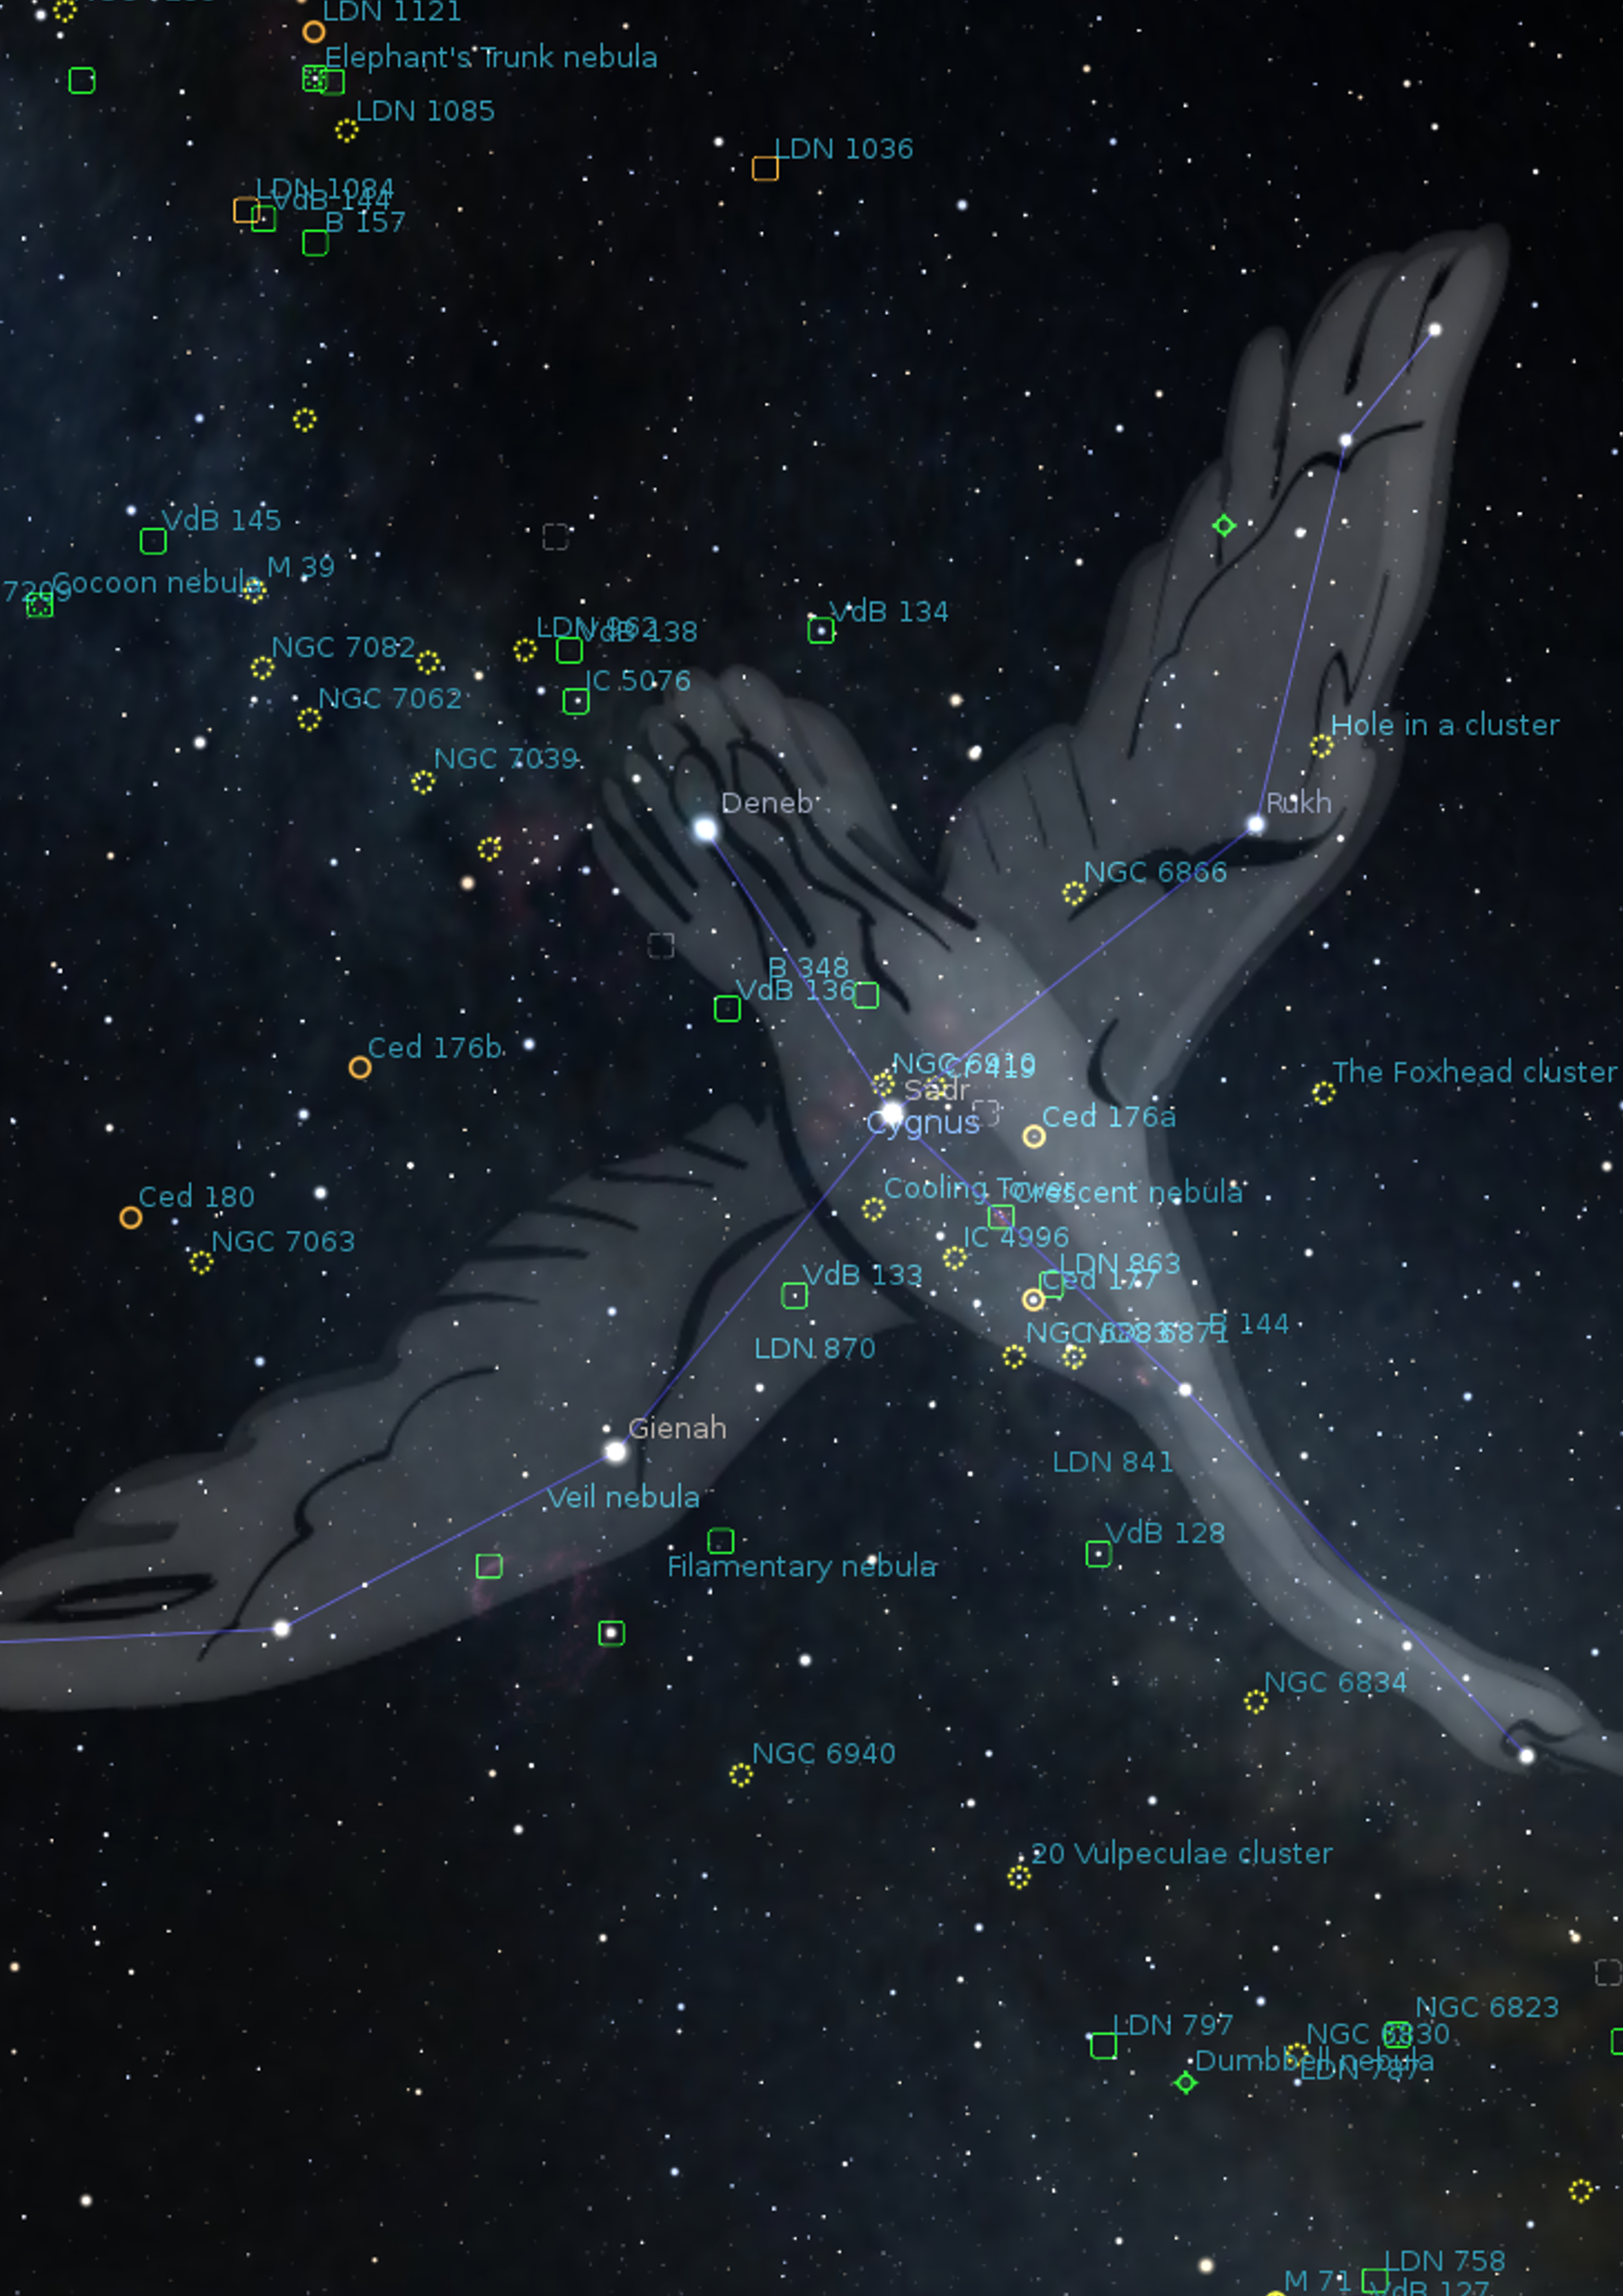
\includegraphics[width=\paperwidth]{bookcover}}; % Background image
\draw[anchor=north] (midpoint) node [fill=ocre!30!white,fill opacity=0.6,text opacity=1,inner sep=1cm]%
     {\Huge\centering\bfseries\sffamily\parbox[c][][t]{\paperwidth}%
                                              {\centering Stellarium User Guide\\[18pt] % Book title
                                              {\Large Matthew Gates, Alexander Wolf, Barry Gerdes, Georg Zotti}\\[15pt]% Author names
                                              {\Large Version \StelVersion-\DocumentEdition}\\[15pt]% Version like 0.15.0-1
                                              {\Large 2016}% Year
                                             }}; % 
\end{tikzpicture}};
\end{tikzpicture}
\vfill
\endgroup

%----------------------------------------------------------------------------------------
%	COPYRIGHT PAGE
%----------------------------------------------------------------------------------------

\newpage
~\vfill
\thispagestyle{empty}

\noindent Copyright \copyright\ 2006-2009 Matthew Gates.\\ % Copyright notice
\noindent Copyright \copyright\ 2011-2016 Alexander Wolf.\\ % Copyright notice
\noindent Copyright \copyright\ 2013-2014 Barry Gerdes.\\ % Copyright notice
\noindent Copyright \copyright\ 2014-2016 Georg Zotti.\\ % Copyright notice

\noindent \textsc{stellarium.org}\\ % URL

\noindent Permission is granted to copy, distribute and/or modify this
document under the terms of the GNU Free Documentation License,
Version 1.2 or any later version published by the Free Software
Foundation; with no Invariant Sections, no Front-Cover Texts, and no
Back-Cover Texts. A copy of the license is included in
section~\ref{ch:License} entitled ``GNU Free Documentation
License''.\\ % License information

\noindent \textit{A draft of version 0.15.0-1, \today} % Printing/edition date

%----------------------------------------------------------------------------------------
%	TABLE OF CONTENTS
%----------------------------------------------------------------------------------------

\chapterimage{chapter-t1-bg} % Table of contents heading image

\pagestyle{empty} % No headers

\tableofcontents % Print the table of contents itself

\cleardoublepage % Forces the first chapter to start on an odd page so it's on the right

\pagestyle{fancy} % Print headers again


%% There should be one source file per chapter. 
%% Structural changes (chapter images etc.) should be in this main file to better have an overview.
%----------------------------------------------------------------------------------------
%	PART I
%----------------------------------------------------------------------------------------

\part{Basic Use}

%----------------------------------------------------------------------------------------
%	CHAPTER 1 (Introduction)
%----------------------------------------------------------------------------------------
\chapterimage{chapter-t2-bg} % Chapter heading image

\chapterimage{chapter-t2-bg} % Chapter heading image

\chapter{Introduction}

\emph{Stellarium} is a software project that allows people to use their
home computer as a virtual planetarium. It calculates the positions of
the Sun and Moon, planets and stars, and draws how the sky would look to
an observer depending on their location and the time. It can also draw
the constellations and simulate astronomical phenomena such as meteor
showers, and solar or lunar eclipses.

Stellarium may be used as an educational tool for teaching about the
night sky, as an observational aid for amateur astronomers wishing to
plan a night's observing, or simply as a curiosity (it's fun!). Because
of the high quality of the graphics that Stellarium produces, it is used
in some real planetarium projector products. Some amateur astronomy
groups use it to create sky maps for describing regions of the sky in
articles for newsletters and magazines.

The development of a powerful scripting system has been continuing for a
number of years now and can now be called operational. The use of a
script was recognised as a perfect way of arranging a display of a
sequence of astronomical events from the earliest versions of Stellarium
and a simple system called the Stratoscript was implemented. The
scipting facility is Stellarium's version of a \emph{Presentation}, a
feature that may be used to run an astronomical or other presentation
for instruction or entertainment from within the Stellarium program. The
original Stratoscript was quite limited in what it could do so a new
Stellarium Scripting System has been developed.

Stellarium is under fairly rapid development, and by the time you read
this guide, a newer version may have been released with even more
features that those documented here. Check for updates to Stellarium at
the Stellarium website.

If you have questions and/or comments about this guide, please email the
author. For comments about Stellarium itself, visit the
\href{https://sourceforge.net/p/stellarium/discussion/278769/}{Stellarium
forums}.



%----------------------------------------------------------------------------------------
%	CHAPTER 2 (Installation)
%----------------------------------------------------------------------------------------
% \chapterimage{chapter-t2-bg} % Chapter heading image Did not change...

% Status info:
% M. Gates	2006-2009
% A. Wolf	2011-2015
% Lee Carré	2011
% ArdWar	2012
% MisterE	2013
% B. Gerdes	2013
% G. Zotti	2014-2015
% Additions inserted from wiki 2015-12-26
% GZ checked grammar and structure, added ANGLE details and Troubleshooting.
% Content OK for 0.15+.
% TODO: Fix a few TODOs noted below.


\chapter{Getting Started}
\label{ch:GettingStarted}

\section{System Requirements}\index{System Requirements}
\label{sec:GettingStarted:SystemRequirements}

Stellarium has been seen to run on most systems where Qt5 is
available, from tiny ARM computers like the Raspberry Pi~2 or Odroid
C1 to big museum installations with multiple projectors. The most
important hardware requirement is a contemporary graphics subsystem.


\subsection{Minimum}
\begin{itemize}
\item Linux/Unix; Windows 7 and later (It may run on Vista, but unsupported. A special version for XP is still available); OS X 10.7.4 and later
\item 3D graphics card which supports OpenGL 3.0 and GLSL 1.3 (2008
  GeForce 8xxx and later, ATI/AMD Radeon HD-2xxx and later; Intel HD
  graphics (Core-i 2xxx and later)) or OpenGL ES 2.0 and GLSL ES 1.0
  (e.g., ARM SBCs like Raspberry Pi~2). On Windows, some older cards
  may be supported via ANGLE when they support DirectX10.
\item 512 MB RAM
\item 250 MB free on disk
\end{itemize}

\subsection{Recommended}
\begin{itemize}
\item Linux/Unix; Windows 7 and later; OS X 10.8.5 and later
\item 3D graphics card which supports OpenGL 3.3 and above and GLSL1.3 and later
\item 1 GB RAM or more
\item 1.5 GB free on disk. (About 3GB extra required for the optional DE431 files.)
\end{itemize}
 A dark room for realistic rendering --- details like the Milky Way, Zodiacal Light or
star twinkling can't be seen in a bright room.


\section{Downloading}\index{Downloading}
\label{sec:GettingStarted:Downloading}

Download the correct package for your operating system directly from the main page,
\url{http://stellarium.org}.

\section{Installation}\index{Installation}
\label{sec:GettingStarted:Installation}

\subsection{Windows}\index{Windows}

\begin{enumerate}
\item Double click on the installer file you downloaded:
\begin{itemize}
\item \file{stellarium-\StelVersion-win64.exe}
\item \file{stellarium-\StelVersion-win32.exe} for Windows x86
\item \file{stellarium-\StelVersion-classic-win32.exe} for XP
\end{itemize}
\item Follow the on-screen instructions.
\end{enumerate}

\subsection{OS X}\index{OS X}

\begin{enumerate}
\item
  Locate the \file{Stellarium-\StelVersion.dmg} file in
  Finder and double click on it or open it using the Disk Utility
  application. Now, a new disk appears on your desktop and Stellarium is
  in it.
\item
  Open the new disk and please take a moment to read the \file{ReadMe} file.
  Then drag \file{Stellarium} to the Applications folder.
\item
  Note: You should copy Stellarium to the Applications folder before
  running it --- some users have reported problems running it directly
  from the disk image (\file{.dmg}).
\end{enumerate}

\subsection{Linux}\index{Linux}

Check if your distribution has a package for Stellarium already --- if
so you're probably best off using it. If not, you can download and build
the source.

For Ubuntu we provide a package repository with the latest stable
releases. Open a terminal and type:

\begin{commands}
sudo add-apt-repository ppa:stellarium/stellarium-releases
sudo apt-get update
sudo apt-get install stellarium
\end{commands}


\section{Running Stellarium}\index{Running Stellarium}
\label{sec:GettingStarted:Running}

\subsection{Windows}\index{Windows}
\label{sec:GettingStarted:Running:Windows}

The Stellarium installer creates a whole list of items in the
\textbf{Start Menu} under the \textbf{Programs/Stellarium}
section. The list evolves over time, not all entries listed here 
may be installed on your system. Select one of these to run Stellarium:
\begin{description}
  \item[Stellarium] OpenGL version. This is the most efficient for
    modern PCs and should be used when you have installed appropriate
    OpenGL drivers.
  \item[Stellarium (ANGLE mode)] Uses Direct3D translation of the
    OpenGL rendering via ANGLE library. Lets the system decide which
    version of Direct3D is available. In case the system reports
    support for Direct3D~11 but if you experience odd effects like
    missing buttons or planets, directly use
  \item[Stellarium (ANGLE Direct3D 9 mode)] Uses Direct3D translation
    of the OpenGL rendering via ANGLE library. Forces Direct3D
    version~9. \emph{This should be used if you don't see buttons or have
    trouble with other ANGLE modes.}
  \item[Stellarium (ANGLE Direct3D 11 mode)] Uses Direct3D translation
    of the OpenGL rendering via ANGLE library. Forces Direct3D
    version~11. Some systems don't seem to work properly with this.
  \item[Stellarium (ANGLE WARP mode)] Uses DirectX3D~11 software rendering via ANGLE
    library. This should work on any PC without dedicated graphics
    card. However on many systems this fails, it is unclear why.
  \item[Stellarium (MESA mode)] Uses software rendering via MESA
    library. This should work on any PC without dedicated graphics
    card. 
    % TODO This note may be obsolete before 0.15 is out when MESA works again.
    %However on some systems this also fails, it is unclear
    %why\footnote{This was the emergency fallback solution for the 0.13
    %  series. We have reports that 0.13.2-MESA works on a system where
    %  0.14 does not.}
\end{description}
  On startup, a diagnostic check is performed to test whether the
  graphics hardware is capable of running. If all is fine, you will
  see nothing of it.  Else you may see an error panel informing you
  that your computer is not capable of running Stellarium (``No
  OpenGL~2 found''), or that there is only OpenGL~2.1 support. The
  latter means you will be able to see some graphics, but depending on
  the type of issue you will have some bad graphics. For example, on
  an Intel GMA4500 there is only a minor issue in Night Mode, while on
  other systems we had reports of missing planets. If you see this,
  try running in Direct3D~9 or MESA mode, or upgrade your system.

  When you have found a mode that works on your system, you can delete
  the other links.

\subsection{OS X}\index{OS X}
\label{sec:GettingStarted:Running:MacOSX}

Double click on the \emph{Stellarium} application.  Add it to your
\textbf{Dock} for quick access.

\subsection{Linux}\index{Linux}
\label{sec:GettingStarted:Running:Linux}

If your distribution had a package you'll probably already have an
item in the GNOME or KDE application menus. If not, just use a open a
terminal and type \texttt{stellarium}.


\subsection{Troubleshooting}
\label{sec:GettingStarted:Running:Troubleshooting}

Stellarium writes startup and other diagnostic messages into a
logfile. Please see section~\ref{sec:FilesAndDirectories} where this
file is located on your system. This file is \emph{essential} in case when
you feel you need to report a problem with your system which has not
been found before.

If you don't succeed in running Stellarium, please see the online
forum\footnote{\url{https://launchpad.net/stellarium}}.  It includes
FAQ (Frequently Asked Questions)\index{FAQ} and a general question
section which may include further hints. Please make sure you have
read and understood the FAQ before asking the same questions again.


%%% Local Variables: 
%%% mode: latex
%%% TeX-PDF-mode: t
%%% TeX-master: "guide"
%%% End: 


%----------------------------------------------------------------------------------------
%	CHAPTER 3 (was called Interface Guide, but is just a first tour.)
%----------------------------------------------------------------------------------------

% Status info:
% M. Gates	2006-2009
% A. Wolf	2011-2014
% B. Gerdes	2013
% Additions inserted from wiki 2015-12-26
% Content OK for 0.12.4.
% 2016-04 GZ started restructuring
% TODO: typo&grammar check

%\chapterimage{chapter-t2-bg} % Chapter heading image (now in guide.tex)

\chapter{A First Tour}
\label{ch:tour}


\begin{figure}[tbh]\centering
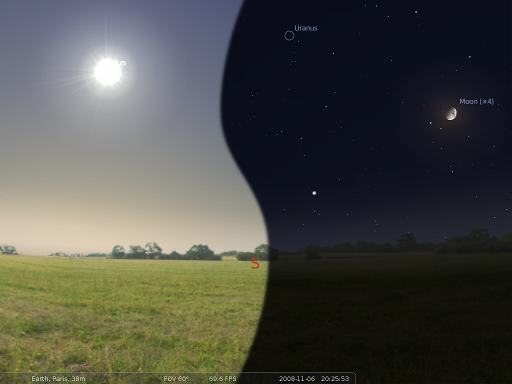
\includegraphics[width=0.95\textwidth,trim=0 0 0 30,clip]{001}
\caption{Stellarium main view. (Combination of day and night views.)}
\label{fig:001}
\end{figure}

\noindent When Stellarium first starts, we see a green meadow under a
sky. Depending on the time of day, it is either a day or night
scene. If you are connected to the Internet, an automatic lookup will
attempt to detect your approximate position.\footnote{See
  section~\ref{sec:gui:location} if you want to switch this off.}

At the bottom left of the screen, you can see the status bar. This shows
the current observer location, field of view (FOV), graphics performance
in frames per second (FPS) and the current simulation date and time.
If you move the mouse over the status bar, it will move up to reveal a
tool bar which gives quick control over the program.

The rest of the view is devoted to rendering a realistic scene including
a panoramic landscape and the sky. If the simulation time and observer
location are such that it is night time, you will see stars, planets and
the moon in the sky, all in the correct positions.

You can drag with the mouse on the sky to look around or use the
cursor keys. You can zoom with the mouse wheel or the \key{Page
  \arrowkeyup} or \key{Page \arrowkeydown} keys.

Much of Stellarium can be controlled very intuitively with the
mouse. Many settings can additionally be switched with shortcut keys
(hotkeys).  Advanced users will learn to use these shortcut
keys. Sometimes a key combination will be used. For example, you can
quit Stellarium by pressing \key{\ctrl+Q} on Windows and Linux, and
\key{\cmdmac+Q} on Mac OS X.  For simplicity, we will show only the
Windows/Linux version. We will present the default hotkeys in this
guide. However, almost all hotkeys can be reconfigured to match your
taste (See~\ref{sec:gui:help:hotkeys}).


The way Stellarium is shown on the screen is primarily governed by the
menus. These are accessed by dragging the mouse to the left or bottom
edge of the screen, where the menus will slide out.


\section{Time Travel}
\label{sec:tour:timeTravel}

When Stellarium starts up, it sets its clock to the same time and date
as the system clock. However, Stellarium's clock is not fixed to the same
time and date as the system clock, or indeed to the same speed. We may
tell Stellarium to change how fast time should pass, and even make time
go backwards! So the first thing we shall do is to travel into the
future! Let's take a look at the time control buttons on the right hand
ride of the tool-bar. If you hover the mouse cursor over the buttons, a
short description of the button's purpose and keyboard shortcut will
appear.

\begin{table}[h]
\centering
\begin{tabular}{c c l}\toprule
\emph{Button} & \emph{Shortcut key} & \emph{Description}\\\midrule
\guibutton[0.75]{2.25}{bt_timerate_decrease} & \key{J} & Decrease the rate at which time passes \\
\guibutton[0.75]{2.25}{bt_timerate_normal}   & \key{K} & Make time pass as normal \\
\guibutton[0.75]{2.25}{bt_timerate_increase} & \key{L} & Increase the rate at which time passes \\
\guibutton[0.75]{2.25}{bt_time_normal}       & \key{8} & Return to the current time \& date \\
\bottomrule
\end{tabular}
\caption{Time Travel}
\end{table}

OK, so lets go see the future! Click the mouse once on the increase time
speed button \guibutton{0.6}{bt_timerate_increase}. 
Not a whole lot seems to happen. However, take a look at the clock in
the status bar. You should see the time going by faster than a normal
clock! Click the button a second time. Now the time is going by faster
than before. If it's night time, you might also notice that the stars
have started to move slightly across the sky. If it's daytime you might
be able to see the sun moving (but it's less apparent than the movement
of the stars). Increase the rate at which time passes again by clicking
on the button a third time. Now time is really flying!

Let time move on at this fast speed for a little while. Notice how the
stars move across the sky. If you wait a little while, you'll see the
Sun rising and setting. It's a bit like a time-lapse movie. 

Stellarium not only allows for moving forward through time -- you can
go backwards too! Click on the real time speed button
\guibutton{0.6}{bt_timerate_normal}.  The stars and/or the
Sun should stop scooting across the sky. Now press the decrease time
speed button \guibutton{0.6}{bt_timerate_decrease} once. Look
at the clock. Time has stopped. Click the Decrease time speed button
four or five more times. Now we're falling back through time at quite
a rate (about one day every ten seconds!).

\subsection*{Time Dragging}
\label{sec:tour:timeDrag}

Another way to quickly change time is \indexterm{time dragging}. Press
\keys{\ctrl+\space} and slide the mouse right to go forward, or left
to go backward.
%% TODO: Apparently stopping or setting to Normal speed is a bit buggy. How to fix that properly?


Enough time travel for now. Wait until it's night time, and then click
the Real time speed button. With a little luck you will now be looking
at the night sky.

\section{Moving Around the Sky}
\label{sec:tour:moving}

\begin{table}[h]
\centering
\begin{tabular}{ll}\toprule
\emph{Key}                         & \emph{Description}\\\midrule
Cursor keys \keys{\arrowkeyleft} \keys{\arrowkeyright} \keys{\arrowkeyup} \keys{\arrowkeydown} & Pan the view left, right, up and down \\
\keyPageUp{}/\keyPageDown{}        & Zoom in and out \\
Backslash (\key{\textbackslash{}}) & Auto-zoom out to original field of view \\
Left mouse button                  & Select an object in the sky \\
Right mouse button                 & Clear selected object \\
Mouse wheel                        & Zoom in and out \\ 
\key{\space}                       & Centre view on selected object \\
Forward-slash (\key{/})            & Auto-zoom in to selected object \\
\bottomrule
\end{tabular}
\caption{Moving Around the Sky}
\label{tab:tour:moving}
\end{table}

As well as travelling through time, Stellarium lets to look around the
sky freely, and zoom in and out. There are several ways to accomplish
this listed in table~\ref{tab:tour:moving}.

Let's try it. Use the cursors to move around left, right, up and down.
Zoom in a little using the \keyPageUp{} key, and back out again using the
\keyPageDown{}. Press the \key{\textbackslash} key and see how Stellarium returns to the
original field of view (how ``zoomed in'' the view is), and direction of
view.
%% TODO Is this still original behaviour? On German Kbd, this does not work anyways, backslash is a AltGr-combination.

It's also possible to move around using the mouse. If you left-click and
drag somewhere on the sky, you can pull the view around.

Another method of moving is to select some object in the sky (left-click
on the object), and press the \key{Space} key to centre the view on that
object. Similarly, selecting an object and pressing the forward-slash
key \key{/} will centre on the object and zoom right in on it.

The forward-slash \key{/} and backslash \key{\textbackslash} keys auto-zoom in an out to different
zoom levels depending on what is selected. If the object selected is a planet
or moon in a \emph{sub-system} with a lot of moons (e.g.\ Jupiter), the
initial zoom in will go to an intermediate level where the whole
sub-system should be visible. A second zoom will go to the full zoom
level on the selected object. Similarly, if you are fully zoomed in on a
moon of Jupiter, the first auto-zoom out will go to the sub-system zoom
level. Subsequent auto-zoom out will fully zoom out and return the
initial direction of view. For objects that are not part of a
sub-system, the initial auto-zoom in will zoom right in on the selected
object (the exact field of view depending on the size/type of the
selected object), and the initial auto-zoom out will return to the
initial FOV and direction of view.

\section{The Main Tool Bar}
\label{sec:tour:toolbar}

\begin{figure}[htb]
\centering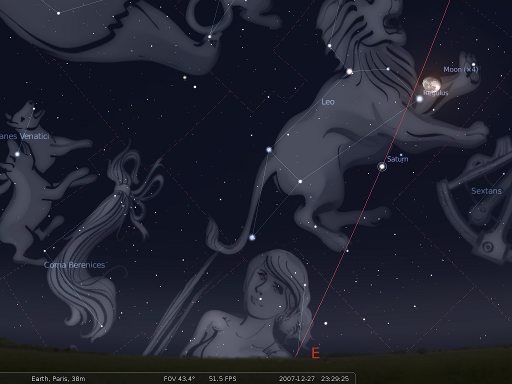
\includegraphics[width=0.9\textwidth]{002}
\caption{Night scene with constellation artwork and moon.}
\label{fig:002}
\end{figure}

Stellarium can do a whole lot more than just draw the stars. Figure~\ref{fig:002}
shows some of Stellarium's visual effects including constellation
line and boundary drawing, constellation art, planet hints, and
atmospheric halo around the bright Moon. The controls in the main tool-bar
provide a mechanism for turning on and off the visual effects.

When the mouse if moved to the bottom left of the screen, a second
tool-bar becomes visible. All the buttons in this side tool-bar open
and close dialog boxes which contain controls for further
configuration of the program. The dialogs will be described in the
next chapter.


Table~\ref{tab:tour:buttons} describes the operations of buttons
on the main tool-bar and the side tool-bar, and gives their default
keyboard shortcuts.

%% TODO: Check default keys!

\begin{longtabu} to \textwidth {llcX}\toprule
\emph{Feature}           & \emph{Button} & \emph{Key} & \emph{Description}\\\midrule
Constellations           & \guibutton[0.75]{2.5}{bt_constellation}     & \key{C} & Draw constellations as ``stick figures'' \\
Constellation Names      & \guibutton[0.75]{2.5}{bt_constellation_name}& \key{V} & Draw name of the constellations \\
Constellation Art        & \guibutton[0.75]{2.5}{bt_constellation_art} & \key{R} & Superimpose artistic representations of the constellations \\
Equatorial Grid          & \guibutton[0.75]{2.5}{bt_eq_grid}           & \key{E} & Draw grid lines for the RA/Dec coordinate system \\
Azimuth Grid             & \guibutton[0.75]{2.5}{bt_az_grid}           & \key{Z} & Draw grid lines for the Alt/Azi coordinate system \\
Toggle Ground            & \guibutton[0.75]{2.5}{bt_ground}            & \key{G} & Toggle drawing of the ground. Turn this off to see objects that are below the horizon. \\
Toggle Cardinal Points   & \guibutton[0.75]{2.5}{bt_cardinal}          & \key{Q} & Toggle marking of the North, South, East and West points on the horizon. \\
Toggle Atmosphere        & \guibutton[0.75]{2.5}{bt_atmosphere}        & \key{A} & Toggle atmospheric effects. Most notably makes the stars visible in the daytime.  \\
Deep-Sky Objects         & \guibutton[0.75]{2.5}{bt_nebulae}           & \key{D} & Toggle marking the positions of Deep-Sky Objects. \\
Planet Hints             & \guibutton[0.75]{2.5}{bt_planets}           & \key{P} & Toggle indicators to show the position of planets. \\
Coordinate System        & \guibutton[0.75]{2.5}{bt_coord_type}        & \key{\ctrl+M} & Toggle between Alt/Azi \& RA/Dec coordinate systems. \\
Goto                     & \guibutton[0.75]{2.5}{bt_goto}              & \key{\Space} & Center the view on the selected object \\
Night Mode               & \guibutton[0.75]{2.5}{bt_night_mode}        & \key{\ctrl+N} & Toggle ``night mode'', which applies a red-only filter to the view to be easier on the dark-adapted eye. \\
Nebula images            & \guibutton[0.75]{2.5}{bt_DSS}        & [none] & Toggle ``nebula images''. This button must be enabled first, see section~\ref{sec:gui:configuration:tools}\\
Full Screen Mode         & \guibutton[0.75]{2.5}{bt_fullscreen} & \key{F11} & Toggle full screen mode. \\
Flip view (horizontal)   & \guibutton[0.75]{2.5}{bt_fliph}      & \key{\ctrl+Shift+H} & Flip the image in the horizontal plane. This button must be enabled first, see section~\ref{sec:gui:configuration:tools} \\
Flip view (vertical)     & \guibutton[0.75]{2.5}{bt_flipv}      & \key{\ctrl+Shift+V} & Flip the image in the vertical plane. This button must be enabled first, see section~\ref{sec:gui:configuration:tools} \\
Quit Stellarium          & \guibutton[0.75]{2.5}{bt_quit}       & \key{\ctrl+Q} & Close Stellarium.\\
Help Window              & \guibutton[0.5]{2.5}{btd_help}       & \key{F1} & Show the help window, with key bindings and other useful information \\
Configuration Window     & \guibutton[0.5]{2.5}{btd_config}     & \key{F2} & Show the configuration window \\ 
Search Window            & \guibutton[0.5]{2.5}{btd_find}       & \key{F3} or \key{Ctrl+F} & Show the object search window \\
View Window              & \guibutton[0.5]{2.5}{btd_view}       & \key{F4} & Show the view window \\
Time Window              & \guibutton[0.5]{2.5}{btd_time}       & \key{F5} & Show the time window \\
Location Window          & \guibutton[0.5]{2.5}{btd_location}   & \key{F6} & Show the observer location window (map) \\
\bottomrule
\caption{Stellarium's standard menu buttons}
\label{tab:tour:buttons}
\end{longtabu}


\section{Taking Screenshots}
\label{sec:tour:screenshots}

You can save what is on the screen to a file by pressing
\key{\ctrl+S}. Screenshots are taken in \file{.png} format, and
have filenames like \file{stellarium-000.png},
\file{stellarium-001.png} (the number increments to prevent
overwriting existing files).

Stellarium creates screenshots in a directory depending on
your operating system, see section
\ref{sec:Directories} Files and Directories.







%%% Local Variables: 
%%% mode: latex
%%% TeX-master: "guide"
%%% End: 



%----------------------------------------------------------------------------------------
%	CHAPTER 4 (was called Configuration, but is really an in-depth description of the panels.)
%----------------------------------------------------------------------------------------

% Status info:
% M. Gates	2006-2009
% A. Wolf	2011-2014
% B. Gerdes	2013
% Additions inserted from wiki 2015-12-26
% Content OK for 0.12.4.
% 2016-04 GZ started restructuring
% TODO: typo&grammar check

% \chapterimage{chapter-t2-bg} % Chapter heading image now set in guide.tex

\chapter{The User Interface}
\label{ch:gui}


This chapter describes the dialog windows which can be accessed from the left menu bar.

Most of Stellarium's settings can be changed using the view window
(press \guibutton[0.35]{2}{btd_view} or \key{F4}) and the
configuration window (\guibutton[0.35]{2}{btd_config} or
\key{F2}). Most settings have short labels. To learn more about some
settings, more information is available as \emph{tooltips}, small text
boxes which appear when you hover the mouse cursor over a
button.\footnote{Unfortunately, on Windows~7 and later, with NVidia
  and AMD GPUs, these tooltips often do not work.}

\newFeature{0.15} You can drag the
windows around, and the position will be used again when you restart
Stellarium. If this would mean the window is off-screen (because you
start in windowed mode, or with a different screen), the window will
be moved so that at least a part is visible.

Some options are really rarely changed and therefore may only be
configured by editing the configuration file.  See
\ref{sec:ConfigurationFile} The Main Configuration File for more
details.



\section{Setting the Date and Time}
\label{sec:gui:date}

\begin{figure}[h]
\centering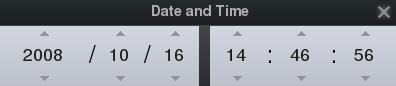
\includegraphics{date_and_time_dialog}
\caption{Date and Time dialog}
\label{fig:gui:date}
\end{figure}

In addition to the time rate control buttons on the main toolbar, you
can use the date and time window (open with the \guibutton[0.35]{2}{btd_time} button or \key{F5}) to set the simulation time. The values
for year, month, day, hour, minutes and seconds may be modified by
typing new values, by clicking the up and down arrows above and below
the values, and by using the mouse wheel.

\subsection{Julian Day Number}
\label{sec:gui:date:julian}

In the 19th century, European astronomers have introduced the use of
Julian Day numbers (invented around the time of the Gregorian calendar
reform). This is a simple continuous day count starting on January 1, -4712
(4713 BC). There are no years, months etc., and the integral day
number switches at noon, so during a single night of observation (in
Europe) the date never changes. 

The fractional part of the number is just the fraction of day that has
elapsed since last noon. Given that a day has 86400~seconds, we should
give a JD with 5 decimal places to capture the nearest second.

This causes a problem for modern computers: even a ``double precision
float'' can keep only about 13 decimal places. More than 2.4 million
days have passed, so that e.g. January 1, 2000, 12:00UT is 2451545.0,
which is an accurately storable number with 7 decimal places, but 12:34:56UT is computed as
2451545.02426. A more accurate result would yield
2451545.024259259259... So, for a field where sub-second accuracy
became crucial like spacecraft operations, the \indexterm{Modified
  Julian Date} (MJD) has been introduced. It is simply
\begin{equation}
  \label{eq:MJD}
  MJD=JD-2400000.5. 
\end{equation}
This means, days start at midnight, and the (constant, in our era)
decimal places of the ``big numbers'' at the begin of the number have
been traded in for more decimal places at the end. 

Don't put your expectations too high when you see MJD displayed:
Stellarium uses JD for internal timekeeping, and Stellarium's display
of MJD is simply computed from it. So you cannot set temporal
increments smaller than a second, and it hardly would make sense to
expect more.

\section{Setting Your Location}
\label{sec:gui:location}

\begin{figure}[htb]
\centering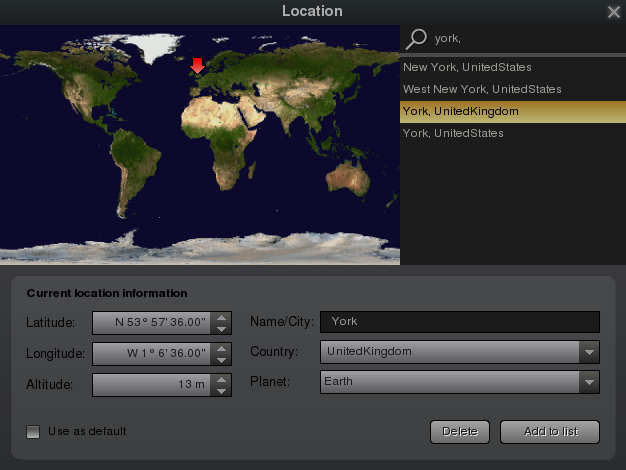
\includegraphics[scale=0.68]{location_dialog}
\caption{Location window}
\label{fig:gui:location}
\end{figure}

The positions of the stars in the sky is dependent on your location on
Earth (or other planet) as well as the time and date. For Stellarium to
show accurately what is (or will be/was) in the sky, you must tell it
where you are. You only need to do this once -- Stellarium can save your
location so you won't need to set it again until you move.

\newFeature{0.13.1}
After installation, Stellarium uses an online service which tries to
find your approximate location based on the IP address you are
using. This seems very practical, but if you feel this causes privacy
issues, you may want to switch this feature off. You should consider
switching it off on a computer which does not move, to save network
bandwidth.

To set your location more accurately, or if the lookup service fails,
press \key{F6} to open the location window. There are a few ways you
can set your location:

\begin{enumerate}
\item Just click on the map.
\item Search for a city where you live using the search edit box at
  the top right of the window, and select the right city from the
  list.
\item Click on the map to filter the list of cities in the vicinity of
  your click, then choose from the shortlist.
\item Enter a new location using the longitude, latitude and other
  data.
\end{enumerate}

\noindent Once you're happy that the location is set correctly, click on the ``use
as default'' checkbox, and close the location window.



\section{The Configuration Window}
\label{sec:gui:configuration}

The configuration window contains general program settings, and many
other settings which do not concern specific display options. Press
the tool button \guibutton[0.35]{2}{btd_config} or \key{F2} to open.


\subsection{The Main Tab}
\label{sec:gui:configuration:main}


\begin{figure}[p]
\centering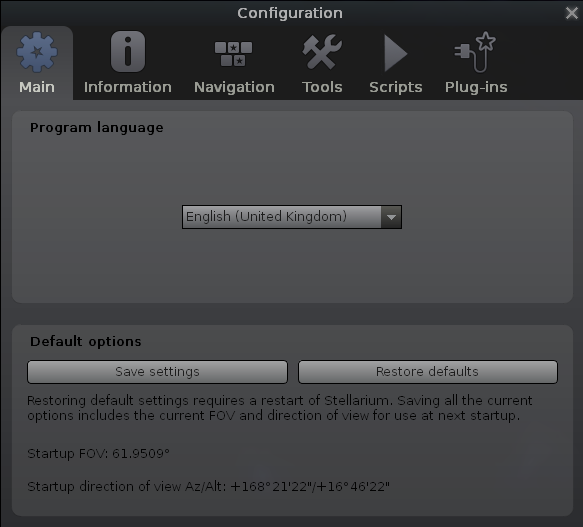
\includegraphics[scale=0.55]{config_dialog_main_tab}
\caption{Configuration Window: Main Tab}
\label{fig:gui:configuration:main}
\end{figure}



The Main tab in the configuration window provides controls for changing
the program language, how much information is shown about selected sky
objects, and provides a button for saving the current program
configuration.

\subsection{The Information Tab}
\label{sec:gui:configuration:info}


\begin{figure}[p]
\centering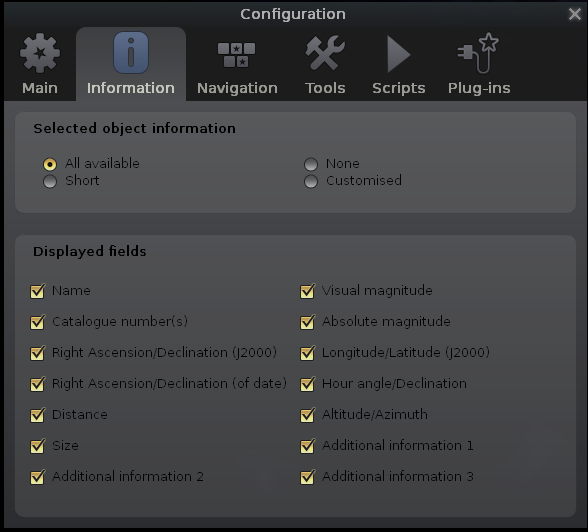
\includegraphics[scale=0.55]{config_dialog_info_tab}
\caption{Configuration Window: Information Tab}
\label{fig:gui:configuration:info}
\end{figure}

The Information tab allows you to set the type and amount of information
displayed about a selected object.
\begin{itemize}
\item Ticking or unticking the relevant boxes will control this.
\item The information displays in various colours depending on the type and
level of the stored data
\end{itemize}

\subsection{The Navigation Tab}
\label{sec:gui:configuration:nav}


\begin{figure}[p]
\centering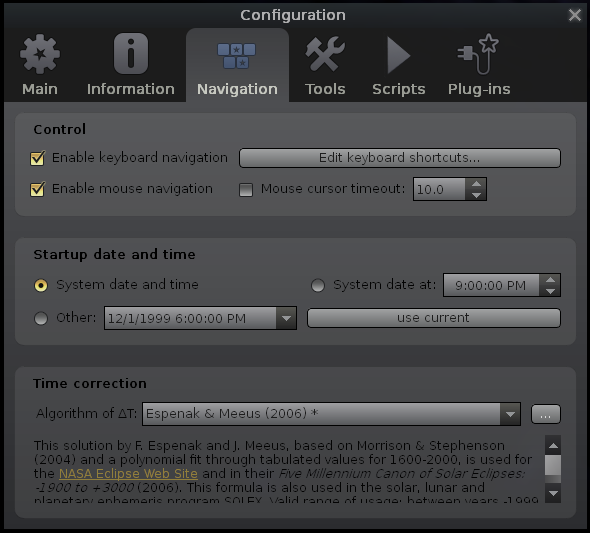
\includegraphics[scale=0.55]{config_dialog_navigation_tab}
\caption{Configuration Window: Navigation Tab}
\label{fig:gui:configuration:nav}
\end{figure}

The Navigation tab (Fig.~\ref{fig:gui:configuration:nav}) allows for
enabling/disabling of keyboard shortcuts for panning and zooming the
main view, and also how to specify what simulation time should be used
when the program starts:

\begin{description}
\item[System date and time] Stellarium will start with
  the simulation time equal to the operating system clock.
\item[System date at] Stellarium will start with the
  same date as the operating system clock, but the time will be fixed at
  the specified value. This is a useful setting for those people who use
  Stellarium during the day to plan observing sessions for the upcoming
  evening.
\item[Other] some fixed time can be chosen which will
  be used every time Stellarium starts.
\end{description}

\subsection{The Tools Tab}
\label{sec:gui:configuration:tools}


\begin{figure}[p]
\centering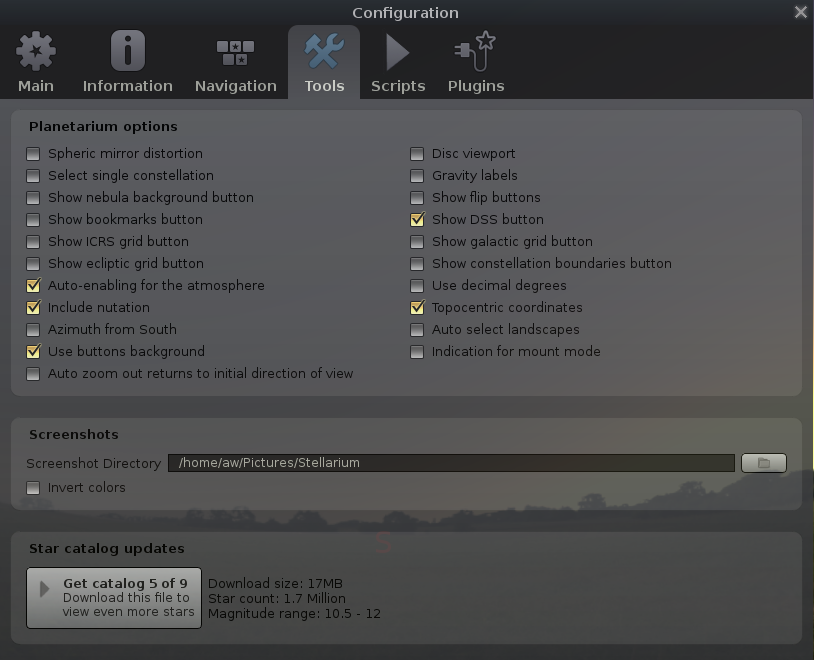
\includegraphics[scale=0.55]{config_dialog_tools_tab}
\caption{Configuration Window: Tools Tab}
\label{fig:gui:configuration:tools}
\end{figure}


The Tools tab (Fig.~\ref{fig:gui:configuration:tools}) contains miscellaneous utility
features:

\begin{description}
\item[Show flip buttons] When enabled, two buttons will be added to
  the main tool-bar which allow the main view to be mirrored in the
  vertical and horizontal directions. This is useful when observing
  through telecopes which may cause the image to be mirrored.
\item[Spheric mirror distortion] This option pre-warps the main view
  such that it may be projected onto a spherical mirror using a
  projector. The resulting image will be refected up from the spherical
  mirror in such a way that it may be shone onto a small planetarium
  dome, making a cheap planetarium projection system.
\item[Disc viewport] This option limits masks the main view
  producing the effect of a telescope eyepiece. It is also useful when
  projecting Stellarium's output with a fish-eye lens planetarium
  projector.
\item[Gravity labels] This option makes labels of objects in the
  main view align with the nearest horizon. This means that labels
  projected onto a dome are always alighned properly.
\item[Auto zoom out returns to initial field of view] When enabled,
  this option changes the behaviour of the zoom out key
  (\textbackslash{}) so that it resets the initial direction of view in
  addition to the field of view.
\end{description}

\subsection{The Scripts Tab}
\label{sec:gui:scripts}


\begin{figure}[p]
\centering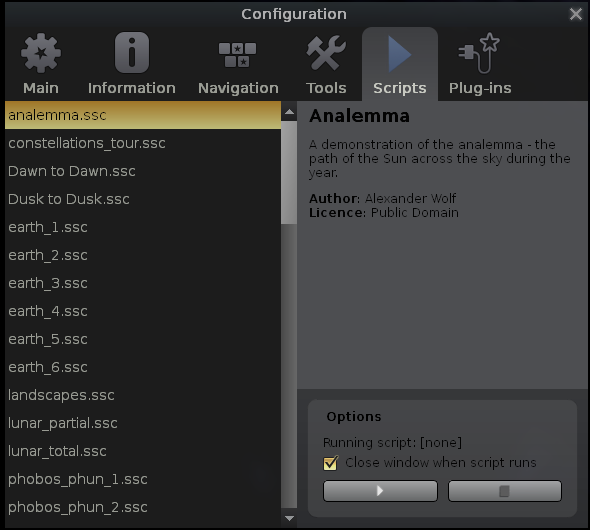
\includegraphics[scale=0.55]{config_dialog_scripts_tab}
\caption{Configuration Window: Scripts Tab}
\label{fig:gui:configuration:scripts}
\end{figure}

The Scripts tab (Fig.~\ref{fig:gui:configuration:scripts}) allows the selection of
pre-assembled scripts bundled with Stellarium that can be run. This
list can be expanded by your own scripts as required. See
section~\ref{sec:FilesAndDirectories:DirectoryStructure} where to
store your own scripts, and chapter~\ref{ch:scripting} for an
introduction to the scripting capabilities and language.

When a script is selected it can be run by pressing the arrow button
and stopped with the stop button. With some scripts the stop button is
inhibited until the script is finished. %% TODO: EXPLAIN HOW?

Scripts that use sound or embedded videos will need a version of
Stellarium compiled at compile time with multimedia support
enabled. It must be pointed out here that sound or video codecs
available depends on the sound and video capabilities of you computer
platform and may not work.


\subsection{The Plugins Tab }
\label{sec:gui:configuration:plugins}


\begin{figure}[p]
\centering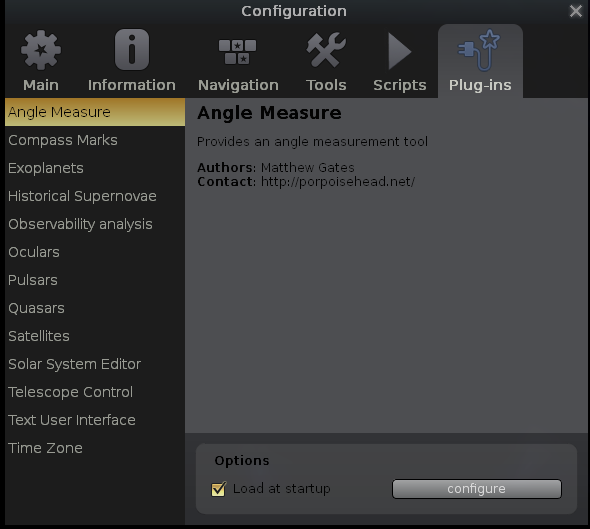
\includegraphics[scale=0.55]{config_dialog_plugins_tab}
\caption{Configuration Window: Plugins}
\label{fig:gui:plugins}
\end{figure}

Plugins (see chapter~\ref{ch:plugins} for an introduction) can be
enabled here (Fig.~\ref{fig:gui:plugins}) to be loaded the next time
you start Stellarium.  Many plugins allow additional configuration
which will be available again on this tab.




\section{The View Settings Window}
\label{sec:gui:view}

The View settings window controls many display features of Stellarium
which are not available via the main toolbar.

\subsection{Sky Tab}
\label{sec:gui:view:sky}

\begin{figure}[t]
\centering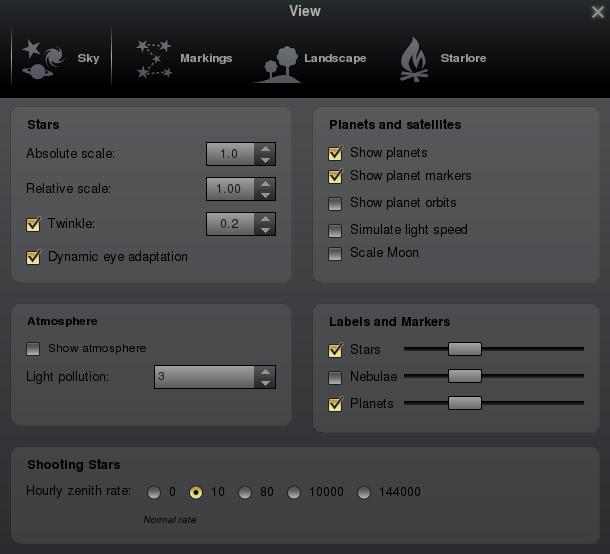
\includegraphics[scale=0.68]{view_dialog_sky_tab}
\caption{View Settings Window: Sky Tab}
\label{fig:gui:view:sky}
\end{figure}

The Sky tab of the View window (Fig.~\ref{fig:gui:view:sky}) contains settings
for changing the general appearane of the main sky view. Some
hightlights:

\begin{description}
\item[Absolute scale] is the size of stars as rendered by
  Stellarium. If you increase this value, all stars will appear larger
  than before.
\item[Relative scale] determines the difference in size of bright
  stars compared to faint stars. Values higher than 1.00 will make the
  brightest stars appear much larger than they do in the sky. This is
  useful for creating star charts, or when learning the basic
  constellations.
\item[Twinkle] controls how much the stars twinkle.
\item[Dynamic eye adaptation] When enabled this feature reduces the
  brightness of faint objects when a bright object is in the field of
  view. This simulates how the eye can be dazzled by a bright object
  such as the moon, making it harder to see faint stars and galaxies.
\item[Light pollution] In urban and suburban areas, the sky is
  brightned by terrestrial light pollution reflected in the atmophere.
  Stellarium simulates light pollution and is calibrated to the
  \emph{Bortle Dark Sky Scale} where 1 means a good dark sky, and 9 is
  a very badly light-polluted sky. See Appendix~\ref{ch:BortleScale}
  for more information.
\item[Planets and satellites] this group of options lets you turn on
  and off various features related to the planets. Simulation of light
  speed will give more precise positions for planetary bodies which move
  rapidly against backround stars (e.g. the moons of Jupiter). The
  \emph{Scale Moon} option will increase the apparent size of the moon
  in the sky, which can be nice for wide field of view shots.
\item[Labels and markers] you can independantly change the amount of
  labels displayed for planets, stars and nebuulae. The further to the
  right the sliders are set, the more labels you will see. Note that
  more labels will also appear as you zoom in.
\item[Shooting stars] Stellarium has a simple meteor simulation
  option. This setting controls how many shooting stars will be shown.
  Note that shooting stars are only visible when the time rate is 1, and
  might not be visiable at some times of day. Meteor showers are not
  currently simulated.
\end{description}

\subsubsection{Atmosphere settings}
\label{sec:gui:view:sky:atmosphere}

An auxiliary dialog contains detail settings for the atmosphere. Here
you can set atmospheric pressure and temperature which influence
refraction (see section~\ref{sec:concepts:Refraction}), and the
opacity factor for extinction, \emph{magnitude loss per airmass} $k$
(see section~\ref{sec:concepts:Extinction}).

\subsection{Markings Tab}
\label{sec:gui:view:markings}

\begin{figure}[t]
\centering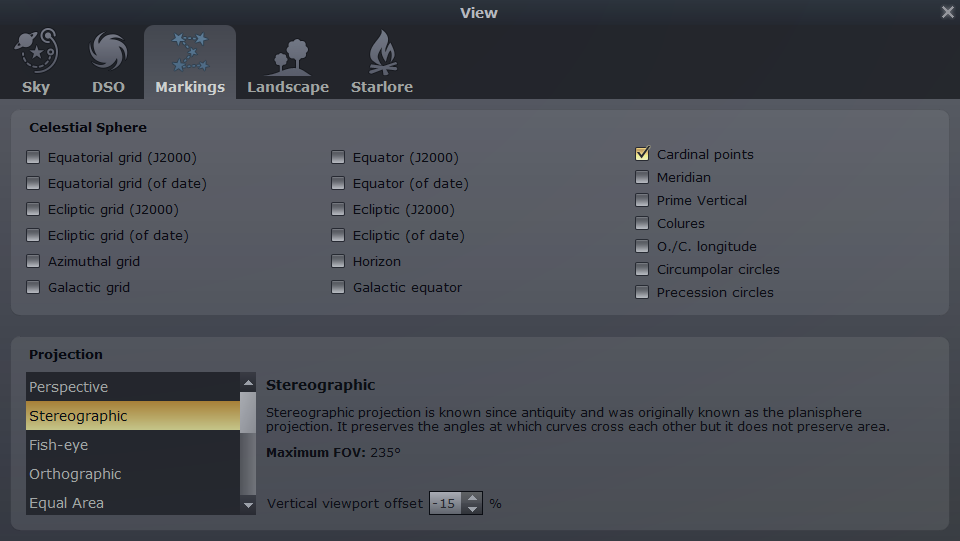
\includegraphics[scale=0.68]{view_dialog_markings_tab}
\caption{View Settings Window: Markings Tab}
\label{fig:gui:view:markings}
\end{figure}

The Markings tab of the View window controls the following features:

\begin{description}
\item[Celestial sphere] this group of options makes it possible to
  plot various grids and lines in the main view.
\item[Constellations] these controls let you turn on and off
  constellation lines, names, art and boundaries, and control the
  brightness of the constellation artwork.
\item[Projection] Selecting items in this list changes the
  projection method which Stellarium uses to draw the sky. Options are:

  \begin{description}
  \item[cylinder] The full name of this projection mode is
    \emph{cylindrical equidistant projection}. The maximum field of view
    in this mode is 233\degree.
  \item[equal area] The full name of this projection method is,
    \emph{Lambert azimuthal equal-area projection}. The maximum field of
    view is 360\degree.
  \item[fish-eye] Stellarium draws the sky using \emph{azimuthal
    equidistant projection}. In fish-eye projection, straight lines
    become curves when they appear a large angular distance from the
    centre of the field of view (like the distortions seen with very
    wide angle camera lenses). This is more pronounced as the user zooms
    out. The maximum field of view in this mode is 180\degree.
  \item[Hammer-Aitoff] The Hammer projection is an equal-area map
    projection, described by Ernst Hammer in 1892 and directly inspired
    by the Aitoff projection. The maximum field of view in this mode is
    360\degree.
  \item[mercator] Mercator projection preserves the angles between
    objects, and the scale around an object the same in all directions.
    The maximum field of view in this mode is 233\degree.
  \item[orthographic] Orthographic projection is related to
    perspective projection, but the \emph{point of perspective} is set
    to an infinite distance. The maximum field of view is 180\degree.
  \item[perspective] Perspective projection keeps the horizon a
    straight line. The maximum field of view is 150\degree. The mathematical
    name for this projection method is \emph{gnomonic projection}.
  \item[stereographic] This mode is similar to fish-eye projection
    mode. The maximum field of view in this mode is 235\degree.
  \end{description}
\end{description}

\subsection{Landscape Tab}
\label{sec:gui:view:landscape}

\begin{figure}[t]
\centering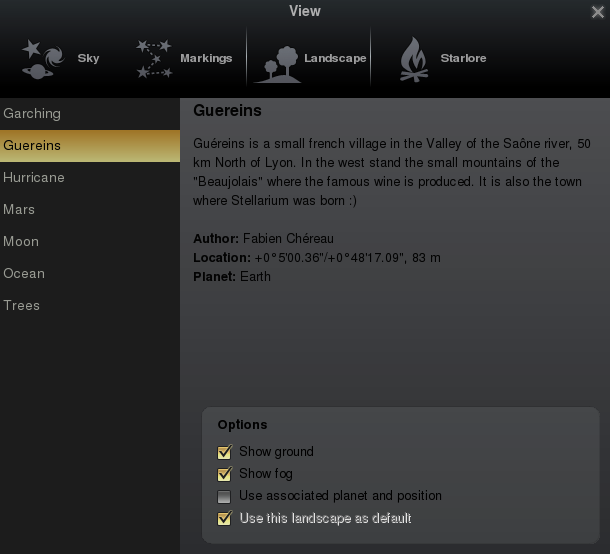
\includegraphics[scale=0.68]{view_dialog_landscape_tab}
\caption{View Settings Window: Landscape Tab}
\label{fig:gui:view:landscape}
\end{figure}

The Landscape tab of the View window controls the landscape graphics
(ground). To change the landscape graphics, select a landscape from the
list on the left side of the window. A description of the landscape will
be shown on the right.

Note that while landscape can include information about where the
landscape graphics were taken (planet, longitude, latitude and
altitude), this location does not have to be the same as the location
selected in the Location window, although you can set up Stellarium such
that selection of a new landscape will alter the location for you.

The controls at the bottom right of the window operate as follows:

\begin{description}
\item[Show ground] This turns on and off landscape rendering (same
  as the button in the main tool-bar).
\item[Show\_fog] This turns on and off rendering of a band of
  fog/haze along the horizon.
\item[Use associated planet and position] When enabled, selecting a
  new landscape will automatically update the observer location.
\item[Use this landscape as default] Selecting this option will save
  the landscape into the program configuration file so that the current
  landscape will be the one used when Stellarium starts.
\end{description}

\subsection{Starlore Tab}
\label{sec:gui:view:starlore}

\begin{figure}[t]
\centering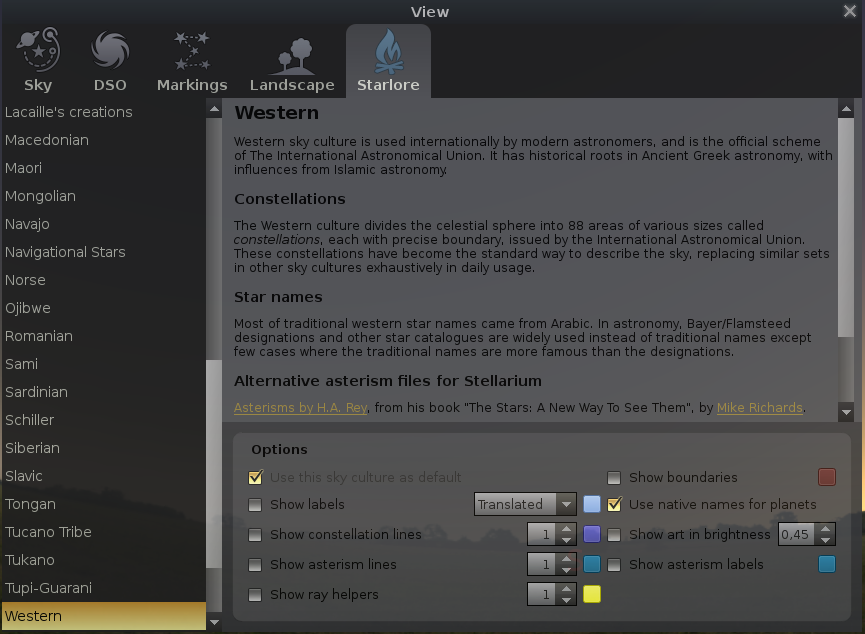
\includegraphics[scale=0.68]{view_dialog_starlore_tab}
\caption{View Settings Window: Starlore Tab}
\label{fig:gui:view:starlore}
\end{figure}

The Starlore tab of the View window controls what culture's
constellations and bright star names will be used in the main display.
Some cultures have constellation art (Western and Inuit), and the rest
do not.


\section{The Object Search Window}
\label{sec:gui:search}

\begin{figure}[p]
\centering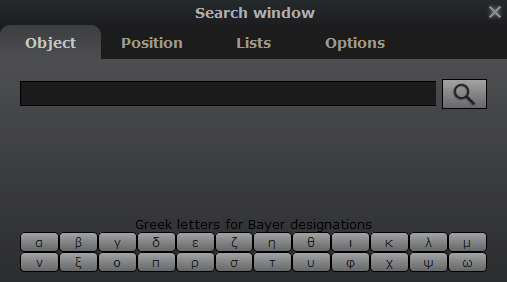
\includegraphics[scale=0.7]{search_dialog}
\caption{The Search Window: Objects}
\label{fig:gui:search}
\end{figure}

\begin{figure}[p]
\centering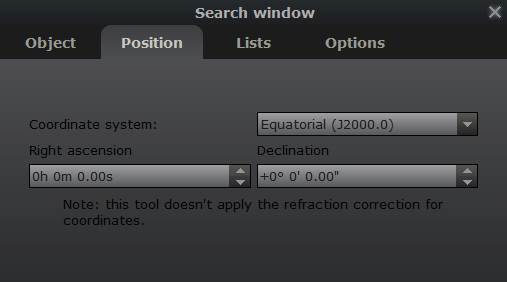
\includegraphics[scale=0.7]{search_dialog_position}
\caption{The Search Window: Positions}
\label{fig:gui:search:position}
\end{figure}

\begin{figure}[p]
\centering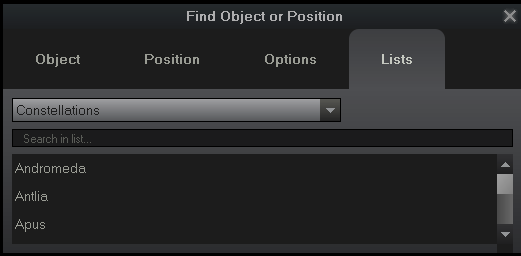
\includegraphics[scale=0.7]{search_dialog_list}
\caption{The Search Window: Lists}
\label{fig:gui:search:position}
\end{figure}


\begin{figure}[p]
\centering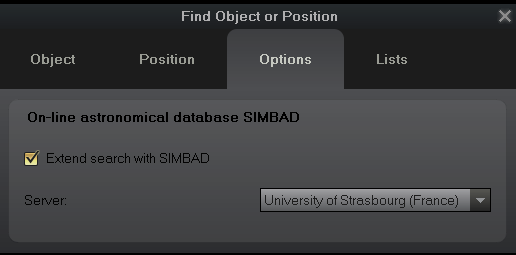
\includegraphics[scale=0.7]{search_dialog_option}
\caption{The Search Window: Options}
\label{fig:gui:search:options}
\end{figure}

The Object Search window provides a convenient way to locate objects in
the sky. Simply type in the name of an object to find, and then click
the \button{go} button or press \key{return}. Stellarium will point you at that
object in the sky.

As you type, Stellarium will make a list of objects which begin with
what you have typed so far. The first of the list of matching objects
will be highlighted. If you press the \key{TAB} key, the selection will change
to the next item in the list. Hitting the \key{RETURN} key will go to the
currently highlighted object and close the search dialog.

For example, suppose we want to locate Mimas (a moon of Saturn). After
typing the first letter of the name, \emph{m}, Stellarium makes a list
of objects whose name begins with M: Mars, Mercury, Mimas, Miranda,
Moon. The first item in this list, Mars, is highlighted. Pressing \key{return}
now would go to Mars, but we want Mimas. We can either press \key{TAB} twice
to highlight Mimas and then hit \key{RETURN}, or we can continue to type the
name until it is the first/only object in the list.


The Position tab provides a convenient way to enter a user set
of coordinates.


The List Search tab allows selection of an object from predefined
sets.  The number of choices is governed by the loaded plug
ins. Simply scroll down the first window to select the type. The name
of an object can then be selected from the list. Press \key{enter} and
stelarium will go to that object.


The Options tab provides a few settings to fine-tune your search experience.
When the name of an object to find is typed in the object
window and you are connected to the internet and ``Extend search'' is
ticked, Stellarium will search the SIMBAD on-line  data bases for its
coordinates. You can then click the \button{go} button or press return.
Stellarium will point you at that object in the sky even if there is no
object displayed on the screen. The SIMBAD server being used can be
selected from the scroll window.


\section{Help Window}
\index{sec:gui:help}

\begin{figure}[htbp]
\centering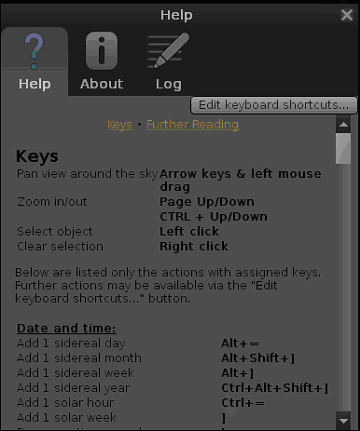
\includegraphics[scale=0.6]{help_dialog}
\caption{Help Window}
\label{fig:gui:help}
\end{figure}

\noindent The Help window lists all of Stellarium's key-strokes. Note that some
features are only available as key strokes, so it's a good idea to have
a browse of the information in this window.

\subsection{Editing Shortcut Keys}
\label{sec:gui:help:hotkeys}

You can edit the shortcut keys here. Each available function can be
configured with up to two key combinations. You may want to
reconfigure keys for example if you have a non-English keyboard layout
and some keys either do not work at all, or feel unintuitive for you,
or if you have other software and want to use the same hotkeys for
similar functions. Simply select the function and click with the mouse
into the edit field, then press your key of choice. If the key has
been taken already, a message will tell you.


\begin{figure}[htbp]
\centering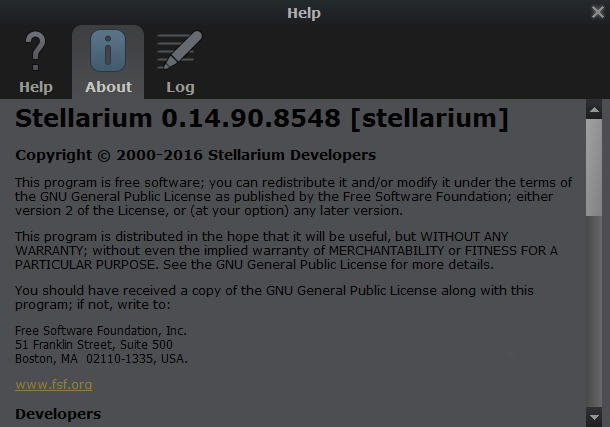
\includegraphics[scale=0.6]{help_dialog_about}
\caption{Help Window: About}
\label{fig:gui:help:about}
\end{figure}

The About tab (Fig.~\ref{fig:gui:help:about}) shows version and licensing information, and a list
of people who helped to produce the program.

\begin{figure}[htbp]
\centering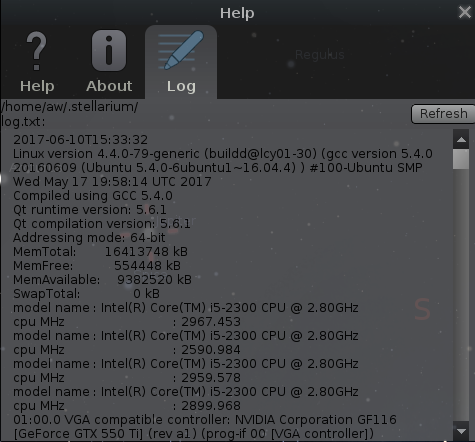
\includegraphics[scale=0.6]{help_dialog_log}
\caption{Help Window: Logfile}
\label{fig:gui:help:log}
\end{figure}

The log tab (Fig.~\ref{fig:gui:help:log}) shows messages like the loading confirmations carried out when
stellarium runs. It is useful to locate the files that stellarium writes
to your computer. The same information is written to  the file \file{log.txt} that you will
find in your user directory (see~\ref{sec:Directories}).




%%% Local Variables: 
%%% mode: latex
%%% TeX-master: "guide"
%%% End: 


%----------------------------------------------------------------------------------------
%	PART II
%----------------------------------------------------------------------------------------

\part{Advanced Use}

%----------------------------------------------------------------------------------------
%	CHAPTER 5 (Advanced Use)
%----------------------------------------------------------------------------------------
\chapterimage{chapter-t3-bg} % Chapter heading image

\chapterimage{chapter-t3-bg} % Chapter heading image

\chapter{Files and Directories}\label{advanced-use}

Stellarium has many data files containing such things as star catalogue
data, nebula images, button icons, font files and configuration files.
When Stellarium looks for a file, it looks in two places. First, it
looks in the \emph{user directory} for the account which is running
Stellarium. If the file is not found there, Stellarium looks in the
\emph{installation directory}\footnote{The installation directory was
  referred to as the config root directory in previous versions of this
  guide}. Thus it is possible for Stellarium to be installed as an
administrative user and yet have a writable configuration file for
non-administrative users. Another benefit of this method is on
multi-user systems: Stellarium can be installed by the administrator,
and different users can maintain their own configuration and other files
in their personal user accounts.

In addition to the main search path, Stellarium saves some files in
other locations, for example screens shots and recorded scripts.

The locations of the user directory, installation directory,
\emph{screenshot save directory} and \emph{script save directory} vary
according to the operating system and installation options used. The
following sections describe the locations for various operating systems.

\section{Windows}\label{windows}

\begin{itemize}
\item
  \textbf{installation directory} By default this is
  \texttt{C:\textbackslash{}Program\ Files\textbackslash{}Stellarium\textbackslash{}},
  although this can be adjusted during the installation process.
\item
  \textbf{user directory} This is the Stellarium sub-folder in the
  Application Data folder for the user account which is used to run
  Stellarium. Depending on the version of Windows and its configuration,
  this could be any of the following (each of these is tried, if it
  fails, the next in the list if tried).
\end{itemize}

\begin{config}
\texttt{\%APPDATA\%\textbackslash{}Stellarium\textbackslash{}}\\
\texttt{\%USERPROFILE\%\textbackslash{}Stellarium\textbackslash{}}\\
\texttt{\%HOMEDRIVE\%\textbackslash{}\%HOMEPATH\%\textbackslash{}Stellarium\textbackslash{}}\\
\texttt{\%HOME\%\textbackslash{}Stellarium\textbackslash{}}\\
\texttt{Stellarium\textbackslash{}s~installation~directory}
\end{config}

Thus, on a typical Windows Vista and Windows 7 systems with user ``Bob
Dobbs'', the user directory will be:

\begin{config}
\texttt{C:\textbackslash{}Users\textbackslash{}Bob~Dobbs\textbackslash{}AppData\textbackslash{}Roaming\textbackslash{}Stellarium\textbackslash{}}
\end{config}



\begin{itemize}
\item
  \textbf{screenshot save directory} Screenshots will be saved to the
  Desktop, although this can be changed with a command line option (see
  section \href{Advanced_Use\#Command_Line_Options}{Command Line
  Options}\footnote{Windows Vista users who do not run Stellarium with
    administrator priviliges should adjust the shortcut in the start
    menu to specify a different directory for screenshots as the Desktop
    directory is not writable for normal progams. The next release of
    Stellarium will include a GUI option to specify the screenshot
    directory.}).
\end{itemize}

\section{Mac OS X}\label{mac-os-x}

\begin{itemize}
\item
  \textbf{installation directory} This is found inside the application
  bundle, \texttt{Stellarium.app}. See the
  \href{http://www.mactipsandtricks.com/articles/Wiley_HT_appBundles.lasso}{Inside
  Application Bundles} for more information.
\item
  \textbf{user directory} This is the
  \texttt{Library/Preferences/Stellarium/} (or
  \texttt{\textasciitilde{}/Library/Application\ Support/Stellarium} on
  newest versions of Mac OS X) sub-directory of the users home
  directory.
\item
  \textbf{screenshot save directory} Screenshots are saved to the users
  Desktop.
\end{itemize}

\section{Linux}\label{linux}

\begin{itemize}
\item
  \textbf{installation directory} This is in the
  \texttt{share/stellarium} sub-directory of the installation prefix,
  i.e. usually \texttt{/usr/share/stellarium} or
  \texttt{/usr/local/share/stellarium/}.
\item
  \textbf{user directory} This is the \texttt{.stellarium} sub-directory
  of users home directory, i.e. \texttt{\textasciitilde{}/.stellarium/}.
\item
  \textbf{screenshot save directory} Screenshots are saved to the users
  home directory.
\end{itemize}

\section{Directory Structure}\label{directory-structure}

Within the \emph{installation directory} and \emph{user directory}
(defined in section \href{Advanced_Use\#Files_and_Directories}{Files and
Directories}), files are arranged in the following sub-directories.

\begin{itemize}
\item
  \textbf{landscapes/} contains data files and textures used for
  Stellarium's various landscapes. Each landscape has it's own
  sub-directory. The name of this sub-directory is called the
  \emph{landscape ID}, which is used to specify the default landscape in
  the main configuration file.
\item
  \textbf{skycultures/} contains constellations, common star names and
  constellation artwork for Stellarium's many sky cultures. Each culture
  has it's own sub-directory in the skycultures directory.
\item
  \textbf{nebulae/} contains data and image files for nebula textures.
  In future Stellarium will be able to support multiple sets of nebula
  images and switch between them at runtime. This feature is not
  implemented for version 0.9.1, although the directory structure is in
  place - each set of nebula textures has it's own sub-directory in the
  nebulae directory.
\item
  \textbf{stars/} contains Stellarium's star catalogues. In future
  Stellarium will be able to support multiple star catalogues and switch
  between them at runtime. This feature is not implemented for version
  0.10.0, although the directory structure is in place - each star
  catalogue has it's own sub-directory in the stars directory.
\item
  \textbf{data/} contains miscellaneous data files including fonts,
  solar system data, city locations etc.
\item
  \textbf{textures/} contains miscellaneous texture files, such as the
  graphics for the toolbar buttons, planet texture maps etc.
\end{itemize}

If any file exists in both the installation directory and user
directory, the version in the user directory will be used. Thus it is
possible to override settings which are part of the main Stellarium
installation by copying the relevant file to the user area and modifying
it there.

It is also possible to add new landscapes by creating the relevant files
and directories within the user directory, leaving the installation
directory unchanged. In this manner different users on a multi-user
system can customise Stellarium without affecting the other users.

\chapter{The Main Configuration
File}\label{the-main-configuration-file}

The main configuration file is read each time Stellarium starts up, and
settings such as the observer's location and display preferences are
taken from it. Ideally this mechanism should be totally transparent to
the user - anything that is configurable should be configured ``in'' the
program GUI. However, at time of writing Stellarium isn't quite complete
in this respect, despite improvements in version 0.10.0. Some settings
can only be changed by directly editing the configuration file. This
section describes some of the settings a user may wish to modify in this
way, and how to do it.

If the configuration file does not exist in the \emph{user directory}
when Stellarium is started (e.g. the first time the user starts the
program), one will be created with default values for all settings
(refer to section \href{Advanced_Use\#Files_and_Directories}{Files and
Directories} for the location of the user directory on your operating
system). The name of the configuration file is
\texttt{config.ini}\footnote{It is possible to specify a different name
  for the main configuration file using the \texttt{-\/-config-file}
  command line option. See section
  \href{Advanced_Use\#Command_Line_Options}{Command Line Options} for
  details.}.

The configuration file is a regular text file, so all you need to edit
it is a text editor like \emph{Notepad} on Windows, \emph{Text Edit} on
the Mac, or \emph{nano/vi/gedit} etc. on Linux.

The following sub-sections contain details on how to make commonly used
modifications to the configuration file. A complete list of
configuration file options and values may be found in the appendix,
\href{Configuration_file}{Configuration file}.

\chapter{Command Line Options}\label{command-line-options}

Stellarium's behaviour can be modified by providing parameters to the
program when it is run, via the command line. See table for a full list:

\begin{longtabu} to \textwidth {l|l|X}
\toprule
\emph{Option} & \emph{Option Parameter} & \emph{Description}\tabularnewline
\midrule
-\/-help or -h & {[}none{]} & Print a quick command line help message
and exit. \tabularnewline
\midrule
-\/-version or -v & {[}none{]} & Print the program name and version
information, and exit. \tabularnewline
\midrule
-\/-config-file or -c & config file name & Specify the configuration
file name. The default value is \texttt{config.ini}.

The parameter can be a full path (which will be used verbatim) or a
partial path.

Partial paths will be searched for inside the regular search paths
unless they start with a ``\texttt{.}'', which may be used to explicitly
specify a file in the current directory or similar.

For example, using the option \texttt{-c\ my\_config.ini} would resolve
to the file
\texttt{\textless{}user\ directory\textgreater{}/my\_config.ini} whereas
\texttt{-c\ ./my\_config.ini} can be used to explicitly say the file
\texttt{my\_config.ini} in the current working directory.
\tabularnewline
\midrule
-\/-restore-defaults & {[}none{]} & If this option is specified
Stellarium will start with the default configuration. Note: The old
configuration file will be overwritten. \tabularnewline
\midrule
-\/-user-dir & path & Specify the user data directory. \tabularnewline
\midrule
-\/-screenshot-dir & path & Specify the directory to which screenshots
will be saved. \tabularnewline
\midrule
-\/-full-screen & yes or no & Over-rides the full screen setting in the
config file. \tabularnewline
\midrule
-\/-home-planet & planet & Specify observer planet (English name).
\tabularnewline
\midrule
-\/-altitude & altitude & Specify observer altitude in meters.
\tabularnewline
\midrule
-\/-longitude & longitude & Specify latitude, e.g. +53d58'16.65"
\tabularnewline
\midrule
-\/-latitude & latitude & Specify longitude, e.g. -1d4'27.48"
\tabularnewline
\midrule
-\/-list-landscapes & {[}none{]} & Print a list of available landscape
IDs. \tabularnewline
\midrule
-\/-landscape & landscape ID & Start using landscape whose ID matches
the passed parameter (dir name for landscape). \tabularnewline
\midrule
-\/-sky-date & date & The initial date in \texttt{yyyymmdd} format.
\tabularnewline
\midrule
-\/-sky-time & time & The initial time in \texttt{hh:mm:ss} format.
\tabularnewline
\midrule
-\/-startup-script & script name & The name of a script to run after the
program has started. \tabularnewline
\midrule
-\/-fov & angle & The initial field of view in degrees. \tabularnewline
\midrule
-\/-projection-type & ptype & The initial projection type (e.g.
\texttt{perspective}). \tabularnewline
\midrule
-\/-dump-opengl-details or -d & {[}none{]} & Dump information about
OpenGL support to logfile. Use this is you have graphics problems and
want to send a bug report. \tabularnewline
\midrule
-\/-angle-mode or -a & {[}none{]} & Use ANGLE as OpenGL ES2 rendering
engine (autodetect driver).\footnote{On Windows only}\tabularnewline
\midrule
-\/-angle-d3d9 or -9 & {[}none{]} & Force use Direct3D 9 for ANGLE
OpenGL ES2 rendering engine.\footnotemark[4]\tabularnewline
\midrule
-\/-angle-d3d11 & {[}none{]} & Force use Direct3D 11 for ANGLE OpenGL
ES2 rendering engine.\footnotemark[4]\tabularnewline
\midrule
-\/-angle-warp & {[}none{]} & Force use the Direct3D 11 software
rasterizer for ANGLE OpenGL ES2 rendering engine.\footnotemark[4]\tabularnewline
\midrule
-\/-mesa-mode or -m & {[}none{]} & Use MESA as software OpenGL rendering
engine.\footnotemark[4]\tabularnewline
\midrule
-\/-safe-mode or -s & {[}none{]} & Synonymous to -\/-mesa-mode.\footnotemark[4]\tabularnewline
\bottomrule
\end{longtabu}

\section{Examples}\label{examples}

\begin{itemize}
\item
  To start Stellarium using the configuration file,
  configuration\_one.ini situated in the user directory (use either of
  these):
\end{itemize}

\texttt{stellarium~-\/-config-file=configuration\_one.ini}\\
\texttt{stellarium~-c~configuration\_one.ini}

\begin{itemize}
\item
  To list the available landscapes, and then to start using the
  landscape with the ID, ``ocean''
\end{itemize}

\texttt{stellarium~-\/-list-landscapes}\\
\texttt{stellarium~-\/-landscape=ocean}

\chapter{Getting Extra Data}\label{getting-extra-star-data}

Stellarium is packaged with over 600 thousand stars in the normal
program download, but much larger star catalogues may be downloaded
using the tool which is in the \emph{Tools} tab of the
\emph{Configuration} dialog.

\chapter{Visual Effects}\label{visual-effects}

\section{Light Pollution}\label{light-pollution}

Stellarium can simulate light pollution, which is controlled from the
light pollution section of the \emph{Sky} tab of the \emph{View} window.
Light pollution levels are set using an numerical value between 1 and 9
which corresponds to the \emph{Bortle Dark Sky Scale}.

\subsection{Excellent dark sky site}
\textbf{Level:} 1 \\
\textbf{Colour:} black \\
\textbf{Limiting magnitude (eye):} 7.6 -- 8.0

Zodiacal light, gegenschein, zodiacal band visible; M33 direct vision naked-eye object; Scorpius and Sagittarius regions of the Milky Way cast obvious shadows on the ground; Airglow is readily visible; Jupiter and Venus affect dark adaptation; surroundings basically invisible.

\subsection{Typical truly dark site}
\textbf{Level:} 2 \\
\textbf{Colour:} grey \\
\textbf{Limiting magnitude (eye):} 7.1 -- 7.5

Airglow weakly visible near horizon; M33 easily seen with naked eye; highly structured Summer Milky Way; distinctly yellowish zodiacal light bright enough to cast shadows at dusk and dawn; clouds only visible as dark holes; surroundings still only barely visible silhouetted against the sky; many Messier globular clusters still distinct naked-eye objects.

\subsection{Rural sky}
\textbf{Level:} 3 \\
\textbf{Colour:} blue \\
\textbf{Limiting magnitude (eye):} 6.6 -- 7.0

Some light pollution evident at the horizon; clouds illuminated near horizon, dark overhead; Milky Way still appears complex; M15, M4, M5, M22 distinct naked-eye objects; M33 easily visible with averted vision; zodiacal light striking in spring and
autumn, color still visible; nearer surroundings vaguely visible.

\subsection{Rural/suburban transition}
\textbf{Level:} 4 \\
\textbf{Colour:} green/yellow \\
\textbf{Limiting magnitude (eye):} 6.1 -- 6.5

Light pollution domes visible in various directions over the horizon; zodiacal light is still visible, but not even halfway extending to the zenith at dusk or dawn; Milky Way above the horizon still impressive, but lacks most of the finer details; M33 a difficult averted vision object, only visible when higher than 55$\degree$; clouds illuminated in the directions of the light sources, but still dark overhead; surroundings clearly visible, even at a distance.

\subsection{Suburban sky}
\textbf{Level:} 5 \\
\textbf{Colour:} orange \\
\textbf{Limiting magnitude (eye):} 5.6 -- 6.0

Only hints of zodiacal light are seen on the best nights in autumn and spring; Milky Way is very weak or invisible near the horizon and looks washed out overhead; light sources visible in most, if not all, directions; clouds are noticeably brighter than the sky.

\subsection{Bright suburban sky}
\textbf{Level:} 6 \\
\textbf{Colour:} red \\
\textbf{Limiting magnitude (eye):} 5.1 -- 5.5

Zodiacal light is invisible; Milky Way only visible near the zenith; sky within 35$\degree$ from the horizon glows grayish white; clouds anywhere in the sky appear fairly bright; surroundings easily visible; M33 is impossible to see
without at least binoculars, M31 is modestly apparent to the unaided eye.

\subsection{Suburban/urban transition}
\textbf{Level:} 7 \\
\textbf{Colour:} red \\
\textbf{Limiting magnitude (eye):} 5.0 at best

Entire sky has a grayish-white hue; strong light sources evident in all directions; Milky Way invisible; M31 and M44 may be glimpsed with the naked eye, but are very indistinct; clouds are brightly lit; even in moderate-sized telescopes the brightest Messier objects are only ghosts of their true selves.

\subsection{City sky}
\textbf{Level:} 8 \\
\textbf{Colour:} white \\
\textbf{Limiting magnitude (eye):} 4.5 at best

Sky glows white or orange --- you can easily read; M31 and M44 are barely glimpsed by an experienced observer on good nights; even with telescope, only bright Messier objects can be detected; stars forming familiar constellation patterns may be weak or completely invisible.

\subsection{Inner City sky}
\textbf{Level:} 9 \\
\textbf{Colour:} white \\
\textbf{Limiting magnitude (eye):} 4.0 at best

Sky is brilliantly lit with many stars forming constellations invisible and many weaker
constellations invisible; aside from Pleiades, no Messier object is visible to the naked eye; only objects to provide fairly pleasant views are the Moon, the Planets and a few of the brightest star clusters.

\chapter{Taking Screenshots}\label{taking-screenshots}

You can save what is on the screen to a file by pressing
\textbf{Control-S}. Screenshots are taken in \emph{.png} format, and
have filenames something like this: \emph{stellarium-000.png},
\emph{stellariuim-001.png} (the number increments to prevent
over-writing existing files).

Stellarium creates screenshots in different directories depending in
your system type, see section
\href{Advanced_Use\#Files_and_Directories}{Files and Directories}.

\chapter{Customising Landscapes}\label{customising-landscapes}

It is possible to create your own landscapes for Stellarium. There are
four types of landscape:

\begin{itemize}
\item
  \textbf{Polygonal Method} Using a text file with azimuths/altitudes.
\item
  \textbf{Single Fish-eye Method} Using a fish-eye panorama image.
\item
  \textbf{Single Spherical Method} Using a spherical panorama image.
\item
  \textbf{Multiple Image Method} (\textbf{also called ``old style''
  landscapes}) Using a series of images split from a 360$\degree$ ``strip''
  panorama image + a ground image.
\end{itemize}

Each landscape has its own sub-directory in
\texttt{\textless{}user\ directory\textgreater{}/landscapes} or
\texttt{\textless{}installation\ directory\textgreater{}/landscapes}.
The name of the sub-directory is called the \emph{landscape ID}. The
sub-directory must contain a file called \texttt{landscape.ini} which
describes the landscape type, texture filenames and other data. Texture
files for a landscape should by put in the same directory as the
\texttt{landscape.ini} file, although if they are not found there they
will be searched for in the \texttt{.../textures} directory, allowing
shared files for common textures such as the generic fog texture.

For example, the \emph{Moon} landscape that is provided with Stellarium
has the following files:

\texttt{.../landscapes/moon/landscape.ini}\\
\texttt{.../landscapes/moon/apollo17.png}

The \texttt{landscape.ini} file must contain a section called
\texttt{{[}landscape{]}}, which contains the details necessary to render
the landscape (which vary, depending on the type of the landscape).

There is also an optional \texttt{{[}location{]}} section which is used
to tell Stellarium where the landscape is in the solar system. If the
\texttt{{[}location{]}} section exists, Stellarium can automatically
adjust the location and observing conditions of the observer to match
the landscape.

\subsection{Polygonal Line Method}\label{polygonal-line-method}

This is the technically simplest of the landscapes, but may be used to
describe accurately measured horizon lines. The file that encodes
horizon altitudes can also be used in all other landscape types. If
present there, it will be used to define object visibility (instead of
the opacity of the landscape photo textures) and, if
\texttt{horizon\_line\_color} is defined, will be plotted.

There is a small caveat: Sometimes, there may appear vertical lines from
some corners towards the zenith or the mathematical horizon, e.g. if
there is a vertex including azimuth 0 or 180. If this irritates you,
just offset this azimuth minimally (e.g., 180.00001).

The \texttt{landscape.ini} file for a polygonal type landscape looks
like this (this example is based on the Geneve landscape which was
borrowed from Cartes du Ciel and comes with Stellarium):

\begin{config}
\texttt{{[}landscape{]}}\\
\texttt{name~=~Geneve}\\
\texttt{type~=~polygonal}\\
\texttt{author~=~Georg~Zotti;~Horizon~definition~by~Patrick~Chevalley}\\
\texttt{description~=~Horizon~line~of~Geneve.~Demonstrates~compatibility~with~horizon~descriptions~from~~Cartes~du~Ciel.}\\
\texttt{polygonal\_horizon\_list~=~horizon\_Geneve.txt}\\
\texttt{polygonal\_angle\_rotatez~=~0}\\
\texttt{ground\_color~=~.15,.45,.45}\\
\texttt{horizon\_line\_color~=~~.75,.45,.45}
\end{config}

Where:

\begin{itemize}
\item
  \textbf{name} is what appears in the landscape tab of the
  configuration window.
\item
  \textbf{type} identifies the method used for this landscape.
  ``polygonal'' in this case.
\item
  \textbf{author} lists the author(s) responsible for images and
  composition.
\item
  \textbf{description} gives a short description visible in the
  selection panel. The text will be superseded by optional
  \texttt{description.\&lt;lang\&gt;.utf8} files.
\item
  \textbf{polygonal\_horizon\_list} is the name of the horizon data file
  for this landscape.
\item
  \textbf{polygonal\_horizon\_list\_mode} (optional) the two first
  columns in the list are numbers: azimuth and altitude or zenith
  distance, in either degrees or radians or gradians(gon). The value
  must be one of
  \texttt{azDeg\_altDeg\textbar{}azDeg\_zdDeg\textbar{}azRad\_altRad\textbar{}azRad\_zdRad\textbar{}azGrad\_altGrad\textbar{}azGrad\_zdGrad}.
  Default: azDeg\_altDeg
\item
  \textbf{polygonal\_angle\_rotatez} (optional, default=0) Angle
  (degrees) to adjust azimuth. This may be used to apply a (usually)
  small offset rotation, e.g. when you have measured the horizon in a
  grid-based coordinate system like UTM and have to compensate for the
  meridian convergence.
\item
  \textbf{ground\_color} (optional, default=``0,0,0'', i.e., black)
  Color for the area below the horizon line. Each R,G,B component is a
  float within 0..1.
\item
  \textbf{horizon\_line\_color} (optional, default: invisible) used to
  draw a polygonal horizon line. Each R,G,B component is a float within
  0..1.
\item
  \textbf{minimal\_brightness} (optional, default=-1, i.e. use preset
  landscape/minimal\_brightness from global \texttt{config.ini}) Some
  minimum brightness to keep landscape visible.
\item
  \textbf{minimal\_altitude} (optional, default=-2) Some sky elements,
  e.g. stars, are not drawn below this altitude. Under certain
  circumstances you may want to specify something else here. (since
  V0.14)
\end{itemize}

\section{Single Fish-eye Method}\label{single-fish-eye-method}

The \emph{Trees} landscape that is provided with Stellarium is an
example of the single fish-eye method, and provides a good illustration.
The centre of the image is the spot directly above the observer (the
zenith). The point below the observer (the nadir) becomes a circle that
just touches the edges of the image. The remaining areas of the image
(the corners outside the circle) are not used.

The image file should be saved in PNG format with alpha transparency.
Wherever the image is transparent is where Stellarium will render the
sky.

The \texttt{landscape.ini} file for a fish-eye type landscape looks like
this (this example is based on the Trees landscape which comes with
Stellarium):

\begin{config}
\texttt{{[}landscape{]}}\\
\texttt{name~=~Trees}\\
\texttt{type~=~fisheye}\\
\texttt{author~=~Robert~Spearman.~Light~pollution~image:~Georg~Zotti}\\
\texttt{description~=~Trees~in~Greenlake~Park,~Seattle}\\
\texttt{maptex~=~trees\_512.png}\\
\texttt{maptex\_illum~=~trees\_illum\_512.png}\\
\texttt{maptex\_fog~=~trees\_fog\_512.png}\\
\texttt{texturefov~=~210}\\
\texttt{angle\_rotatez~=~17}\\
\texttt{tesselate\_rows~=~28}\\
\texttt{tesselate\_cols~=~60}
\end{config}

Where:

\begin{itemize}
\item
  \textbf{name} is what appears in the landscape tab of the
  configuration window.
\item
  \textbf{type} identifies the method used for this landscape.
  ``fisheye'' in this case.
\item
  \textbf{author} lists the author(s) responsible for images and
  composition.
\item
  \textbf{description} gives a short description visible in the
  selection panel. The text will be superseded by optional
  \texttt{description.\&lt;lang\&gt;.utf8} files.
\item
  \textbf{maptex} is the name of the image file for this landscape.
\item
  \textbf{maptex\_fog} (optional) is the name of the fog image file for
  this landscape.
\item
  \textbf{maptex\_illum} (optional) is the name of the nocturnal
  illumination/light pollution image file for this landscape.
\item
  \textbf{texturefov} is the field of view that the image covers in
  degrees.
\item
  \textbf{angle\_rotatez} (optional) Angle (degrees) to adjust azimuth.
\item
  \textbf{tesselate\_rows} (optional, default=20) If straight edges in
  your landscape appear broken, try increasing.
\item
  \textbf{tesselate\_cols} (optional, default=40) If straight edges in
  your landscape appear broken, try increasing.
\item
  \textbf{polygonal\_horizon\_list} (optional) is the name of the
  (measured) horizon data file for this landscape.
\item
  \textbf{polygonal\_horizon\_list\_mode} (optional) the two first
  columns in the list are numbers: azimuth and altitude or zenith
  distance, in either degrees or radians or gradians(gon). The value
  must be one of
  \texttt{azDeg\_altDeg \textbar{} azDeg\_zdDeg \textbar{} azRad\_altRad \textbar{} azRad\_zdRad \textbar{} azGrad\_altGrad \textbar{} azGrad\_zdGrad}.
  Default: \texttt{azDeg\_altDeg}
\item
  \textbf{polygonal\_angle\_rotatez} (optional, default=0) Angle
  (degrees) to adjust azimuth. This may be used to apply a (usually)
  small offset rotation, e.g. when you have measured the horizon in a
  grid-based coordinate system like UTM and have to compensate for the
  meridian convergence.
\item
  \textbf{horizon\_line\_color} (optional, default: invisible) used to
  draw a polygonal horizon line.
\item
  \textbf{minimal\_brightness} (optional, default=-1, i.e. use preset
  landscape/minimal\_brightness from global \texttt{config.ini}) Some
  minimum brightness to keep landscape visible.
\item
  \textbf{minimal\_altitude} (optional, default=-2) Some sky elements,
  e.g. stars, are not drawn below this altitude. Under certain
  circumstances you may want to specify something else here. (since
  V0.14)
\end{itemize}

\section{Single Panorama Method}\label{single-panorama-method}

This method uses a more usual type of panorama - the kind which is
produced directly from software such as \emph{autostitch} or Hugin
(http://hugin.sourceforge.net/). The panorama file should be copied into
the
\texttt{\textless{}config\ root\textgreater{}/landscapes/\textless{}landscape\_id\textgreater{}}
directory, and a \texttt{landscape.ini} file created. The \emph{Moon}
landscape which comes with Stellarium provides a minimal example of the
contents of a landscape.ini file for a spherical type landscape:

\begin{config}
\texttt{{[}landscape{]}}\\
\texttt{name~=~Moon}\\
\texttt{type~=~spherical}\\
\texttt{maptex~=~apollo17.png}
\end{config}

A more elaborate example is found with the \emph{Grossmugl} landscape:

\begin{config}
\texttt{{[}landscape{]}}\\
\texttt{name~=~Grossmugl}\\
\texttt{type~=~spherical}\\
\texttt{author~=~Guenther~Wuchterl,~Kuffner-Sternwarte.at;~Lightscape:~Georg~Zotti}\\
\texttt{description~=~Field~near~Leeberg,~Grossmugl~(Riesentumulus),~Austria~-~Primary~Observing~Spot~of~the~Grossmugl~Starlight~Oasis~-~}\href{http://starlightoasis.org}{\texttt{http://starlightoasis.org}}\\
\texttt{maptex~=~grossmugl\_leeberg\_crop11.25.png}\\
\texttt{maptex\_top=11.25~}\\
\texttt{maptex\_fog~=~grossmugl\_leeberg\_fog\_crop22.5.png}\\
\texttt{maptex\_fog\_top~=~22.5}\\
\texttt{maptex\_fog\_bottom~=~-22.5}\\
\texttt{maptex\_illum~=~grossmugl\_leeberg\_illum\_crop0.png}\\
\texttt{maptex\_illum\_bottom~=~0}\\
\texttt{angle\_rotatez=-89.1}\\
\texttt{minimal\_brightness~=~0.0075}\\
\texttt{polygonal\_horizon\_list~=~horizon\_grossmugl.txt}\\
\texttt{polygonal\_angle\_rotatez=0}\\
\texttt{horizon\_line\_color~=~~.75,.45,.45}\\
\texttt{minimal\_altitude~=~-1}
\end{config}

Where:

\begin{itemize}
\item
  \textbf{name} is what appears in the landscape tab of the
  configuration window.
\item
  \textbf{type} identifies the method used for this landscape.
  ``spherical'' in this case.
\item
  \textbf{author} lists the author(s) responsible for images and
  composition.
\item
  \textbf{description} gives a short description visible in the
  selection panel. The text will be superseded by optional
  \texttt{description.\&lt;lang\&gt;.utf8} files.
\item
  \textbf{maptex} is the name of the image file for this landscape.
\item
  \textbf{maptex\_top} (optional; default=90) is the altitude angle of
  the top edge.
\item
  \textbf{maptex\_bottom} (optional; default=-90) is the altitude angle
  of the bottom edge. Usually you will not require this, or else there
  will be a hole at your feet. ;-)
\item
  \textbf{maptex\_fog} (optional; default: no fog) is the name of the
  fog image file for this landscape.
\item
  \textbf{maptex\_fog\_top} (optional; default=90) is the altitude angle
  of the top edge of the fog texture. Useful to crop away parts of the
  image to conserve texture memory.
\item
  \textbf{maptex\_fog\_bottom} (optional; default=-90) is the altitude
  angle of the bottom edge.
\item
  \textbf{maptex\_illum} (optional; default: no illumination layer) is
  the name of the nocturnal illumination/light pollution image file for
  this landscape.
\item
  \textbf{maptex\_illum\_top} (optional; default=90) is the altitude
  angle of the top edge, if you have light pollution only close to the
  horizon.
\item
  \textbf{maptex\_illum\_bottom} (optional; default=-90) is the altitude
  angle of the bottom edge.
\item
  \textbf{angle\_rotatez} (optional, default=0) Angle (degrees) to
  adjust azimuth. If 0, the left/right edge is due east.
\item
  \textbf{tesselate\_rows} (optional, default=20) If straight edges in
  your landscape appear broken, try increasing. This is the number of
  rows for the maptex. Fog and illumination textures will have a similar
  vertical angle.
\item
  \textbf{tesselate\_cols} (optional, default=40) If straight edges in
  your landscape appear broken, try increasing.
\item
  \textbf{polygonal\_horizon\_list} (optional) is the name of the
  (measured) horizon data file for this landscape. Can be used to query
  horizon transparency (for accurate object rising/setting times)
\item
  \textbf{polygonal\_horizon\_list\_mode} (optional) the two first
  columns in the list are numbers: azimuth and altitude or zenith
  distance, in either degrees or radians or gradians(gon). The value
  must be one of
  \texttt{azDeg\_altDeg\textbar{}azDeg\_zdDeg\textbar{}azRad\_altRad\textbar{}azRad\_zdRad\textbar{}azGrad\_altGrad\textbar{}azGrad\_zdGrad}.
  Default: \texttt{azDeg\_altDeg}
\item
  \textbf{polygonal\_angle\_rotatez} (optional, default=0) Angle
  (degrees) to adjust azimuth. This may be used to apply a (usually)
  small offset rotation, e.g. when you have measured the horizon in a
  grid-based coordinate system like UTM and have to compensate for the
  meridian convergence.
\item
  \textbf{horizon\_line\_color} (optional, default: invisible) used to
  draw a polygonal horizon line.
\item
  \textbf{minimal\_brightness} (optional, default=-1, i.e. use preset
  landscape/minimal\_brightness from global config.ini) Some minimum
  brightness to keep landscape visible.
\item
  \textbf{minimal\_altitude} (optional, default=-2) Some sky elements,
  e.g. stars, are not drawn below this altitude. Under certain
  circumstances (e.g. for space station panoramas where you may have sky
  below your feet, or for deep valleys/high mountains for efficiency,
  you may want to specify something else here. (since V0.14)
\end{itemize}

To save texture memory, since V0.13 you can trim away the transparent
sky and define the angle \textbf{maptex\_top}. Likewise,
\textbf{fogtex\_top}, \textbf{fogtex\_bottom},
\textbf{maptex\_illum\_top} and \textbf{maptex\_illum\_top}. You should
then stretch the texture to a full power of 2, like 4096x1024. The
easiest method to create perfectly aligned fog and illumination layers
is with an image editor that supports layers like the GIMP or Photoshop.
Fog and Light images should have black background.

\section{Multiple Image Method}\label{multiple-image-method}

The multiple image method works by having a 360 panorama of the horizon
(without wasting too much texture memory with the sky) split into a
number of smaller ``side textures'', and a separate ``ground texture''.
This has the advantage over the single image method that the detail
level of the horizon can be increased further without ending up with a
single very large image file, so this is usable for either very
high-resolution panoramas or for older hardware. The ground texture can
be a lower resolution than the panorama images. Memory usage may be more
efficient because there are no unused texture parts like the corners of
the texture file in the fish-eye method. It is even possible to repeat
the horizon several times (for purely decorative purpose). The side
textures are indeed mapped onto curved (spherical ring or cylinder)
walls, not flat sides as shown here.

\begin{figure}[h]
\centering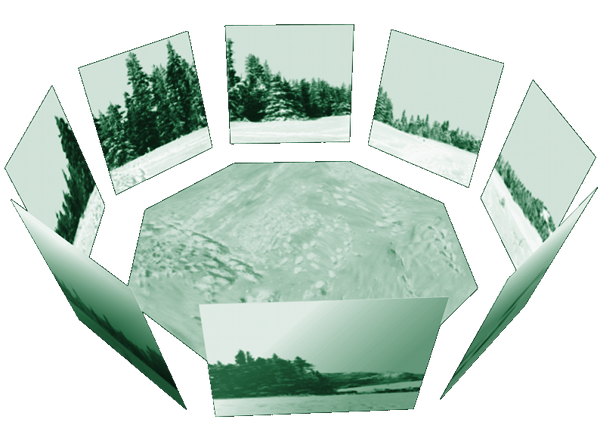
\includegraphics[scale=0.7]{faq_landscape}
%\caption{Figure caption}
\end{figure}

On the negative side, it is more difficult to create this type of
landscape - merging the ground texture with the side textures can prove
tricky. The contents of the \texttt{landscape.ini} file for this
landscape type is also somewhat more complicated than for other
landscape types. Here is the \texttt{landscape.ini} file which describes
the Guereins landscape:

\begin{config}
\texttt{{[}landscape{]}}\\
\texttt{name~=~Guereins}\\
\texttt{type~=~old\_style}\\
\texttt{author~=~Fabien~Chéreau}\\
\texttt{description~=~Guéreins~is~a~small~french~village...}\\
\texttt{nbsidetex~=~8}\\
\texttt{tex0~=~guereins4.png}\\
\texttt{tex1~=~guereins5.png}\\
\texttt{tex2~=~guereins6.png}\\
\texttt{tex3~=~guereins7.png}\\
\texttt{tex4~=~guereins8.png}\\
\texttt{light4~=~guereins8-lgt.png}\\
\texttt{tex5~=~guereins1.png}\\
\texttt{tex6~=~guereins2.png}\\
\texttt{tex7~=~guereins3.png}\\
\texttt{nbside~=~8}\\
\texttt{side0~=~tex0:0:0.005:1:1}\\
\texttt{side1~=~tex1:0:0.005:1:1}\\
\texttt{side2~=~tex2:0:0.005:1:1}\\
\texttt{side3~=~tex3:0:0.005:1:1}\\
\texttt{side4~=~tex4:0:0.005:1:1}\\
\texttt{side5~=~tex5:0:0.005:1:1}\\
\texttt{side6~=~tex6:0:0.005:1:1}\\
\texttt{side7~=~tex7:0:0.005:1:1}\\
\texttt{groundtex~=~guereinsb.png}\\
\texttt{fogtex~=~fog.png}\\
\texttt{nb\_decor\_repeat~=~1}\\
\texttt{decor\_alt\_angle~=~40}\\
\texttt{decor\_angle\_shift~=~-22}\\
\texttt{decor\_angle\_rotatez~=~0}\\
\texttt{ground\_angle\_shift~=~-22}\\
\texttt{ground\_angle\_rotatez~=~45}\\
\texttt{fog\_alt\_angle~=~20}\\
\texttt{fog\_angle\_shift~=~-3}\\
\texttt{draw\_ground\_first~=~1}
\end{config}

Where:

\begin{itemize}
\item
  \textbf{name} is the name that will appear in the landscape tab of the
  configuration window for this landscape
\item
  \textbf{type} should be ``old\_style'' for the multiple image method.
\item
  \textbf{author} lists the author(s) responsible for images and
  composition.
\item
  \textbf{description} gives a short description visible in the
  selection panel. The text will be superseded by optional
  description..utf8 files.
\item
  \textbf{nbsidetex} is the number of side textures for the landscape.
\item
  \textbf{tex0 ... tex} are the side texture file names. These should
  exist in the \texttt{.../textures/landscapes} directory in PNG format.
\item
  \textbf{light0 ... light} are optional textures. If they exist, they
  are used as overlays on top of the respective
  tex\textless{}...\textgreater{} files and represent nocturnal
  illumination, e.g. street lamps, lit windows, red dots on towers, sky
  glow by city light pollution, ... Empty panels don't have to exist. If
  you need your light pollution higher in the sky, you must use a
  spherical or fisheye landscape. (New feature, V0.13.1)
\item
  \textbf{nbside} is the number of side textures
\item
  \textbf{side0 ... side} are the descriptions of how the side textures
  should be arranged in the program. Each description contains five
  fields separated by colon characters (:). The first field is the ID of
  the texture (e.g. tex0), the remaining fields are the texture
  coordinates (x0:y0:x1:y1) used to place the texture in the scene. If
  you want to use all of the image, this will just be \texttt{0:0:1:1}.
\item
  \textbf{groundtex} is the name of the ground texture file. (This could
  also be a diagram e.g. indicating the mountain peaks!)
\item
  \textbf{ground} {[}NO LONGER USED{]} used to be the description of the
  projection of the ground texture in the scene.
\item
  \textbf{fogtex} is the name of the texture file for fog in this
  landscape. Note that for this landscape, accurate overlay of fog and
  landscape is only done if \texttt{calibrated=true} and
  \texttt{tan\_mode=true}.
\item
  \textbf{fog} {[}NO LONGER USED{]} used to be the description of the
  projection of the fog texture in the scene.
\item
  \textbf{nb\_decor\_repeat} is the number of times to repeat the side
  textures in the 360 panorama. (Photo panoramas should have ``1'' here)
\item
  \textbf{decor\_alt\_angle} (degrees) is the vertical angular size of
  the textures (i.e. how high they go into the sky).
\item
  \textbf{decor\_angle\_shift} (degrees) vertical angular offset of the
  scenery textures, at which height are the side textures placed.
\item
  \textbf{decor\_angle\_rotatez} (degrees) angular rotation of the
  scenery around the vertical axis. This is handy for rotating the
  landscape so North is in the correct direction.
\item
  \textbf{ground\_angle\_shift} (degrees) vertical angular offset of the
  ground texture, at which height the ground texture is placed.
\item
  \textbf{ground\_angle\_rotatez} (degrees) angular rotation of the
  ground texture around the vertical axis. When the sides are rotated,
  the ground texture may need to be rotated as well to match up with the
  sides.
\item
  \textbf{fog\_alt\_angle} (degrees) vertical angular size of the fog
  cylinder - how fog looks. Accurate vertical size requires
  \texttt{calibrated=true}.
\item
  \textbf{fog\_angle\_shift} (degrees) vertical angular offset of the
  fog texture - at what height is it drawn. Accurate vertical placement
  requires \texttt{calibrated=true}.
\item
  \textbf{draw\_ground\_first} if 1 the ground is drawn in front of the
  scenery, i.e. the side textures will overlap over the ground texture.
\item
  \textbf{calibrated} (optional, not used in this file). New since
  0.10.6: Only if true, decor\_alt\_angle etc. really work as documented
  above. The (buggy) old code was left to work with the landscapes
  already existing.
\item
  \textbf{tan\_mode} (optional, not used in this file). If true, the
  panorama image must be in in cylindrical, not equirectangular
  projection. Finding \texttt{decor\_alt\_angle} and
  \texttt{decor\_angle\_shift} may be a bit more difficult with this,
  but now (V0.13) works also with calibrated. A fog image created as
  overlay on the pano will be perfectly placed.
\item
  \textbf{decor\_angle\_rotatez} angular rotation of the scenery around
  the vertical axis. This is handy for rotating the landscape so North
  is in the correct direction. If 0, the left edge of \texttt{tex0} is
  due east.
\item
  \textbf{ground\_angle\_shift} vertical angular offset of the ground
  texture, at which height the ground texture is placed. Values above
  -10 are not recommended for non-photographic content due to high
  distortion.
\item
  \textbf{ground\_angle\_rotatez} angular rotation of the ground texture
  around the vertical axis. When the sides are rotated, the ground
  texture may need to be rotated as well to match up with the sides. If
  0, east is up. if North is up in your image, set this to 90.
\item
  \textbf{fog\_alt\_angle} vertical angular size of the fog texture -
  how fog looks.
\item
  \textbf{fog\_angle\_shift} vertical angular offset of the fog texture
  - at what height is it drawn.
\item
  \textbf{draw\_ground\_first} if 1 the ground is drawn before the
  sides, i.e. the side textures may overlap the ground texture if
  \texttt{ground\_angle\_shift\ \&gt;\ decor\_angle\_shift}.
\item
  \textbf{polygonal\_horizon\_list} (optional) is the name of the
  (measured) horizon data file for this landscape. Can be used to query
  horizon transparency (for accurate object rising/setting times)
\item
  \textbf{polygonal\_horizon\_list\_mode} (optional) the two first
  columns in the list are numbers: azimuth and altitude or zenith
  distance, in either degrees or radians or gradians(gon). The value
  must be one of
  azDeg\_altDeg\textbar{}azDeg\_zdDeg\textbar{}azRad\_altRad\textbar{}azRad\_zdRad\textbar{}azGrad\_altGrad\textbar{}azGrad\_zdGrad.
  Default: azDeg\_altDeg
\item
  \textbf{polygonal\_angle\_rotatez} (optional, default=0) Angle
  (degrees) to adjust azimuth. This may be used to apply a (usually)
  small offset rotation, e.g. when you have measured the horizon in a
  grid-based coordinate system like UTM and have to compensate for the
  meridian convergence.
\item
  \textbf{horizon\_line\_color} (optional, default: invisible) used to
  draw a polygonal horizon line.
\item
  \textbf{minimal\_brightness} (optional, default=-1, i.e. use preset
  landscape/minimal\_brightness from global config.ini) Some minimum
  brightness to keep landscape visible.
\item
  \textbf{minimal\_altitude} (optional, default=-2) Some sky elements,
  e.g. stars, are not drawn below this altitude. Under certain
  circumstances you may want to specify something else here. (since
  V0.14)
\end{itemize}

\section{landscape.ini {[}location{]}
section}\label{landscape.ini-location-section}

An example location section:

\begin{config}
\texttt{{[}location{]}}\\
\texttt{planet~=~Earth}\\
\texttt{latitude~=~+48d10'9.707"}\\
\texttt{longitude~=~+11d36'32.508"}\\
\texttt{altitude~=~83}\\
\texttt{light\_pollution=3}\\
\texttt{atmospheric\_extinction\_coefficient=0.2}\\
\texttt{atmospheric\_temperature=10}\\
\texttt{atmospheric\_pressure=-1}
\end{config}

Where:

\begin{itemize}
\item
  \textbf{planet} Is the English name of the solar system body for the
  landscape.
\item
  \textbf{latitude} Is the latitude of site of the landscape in degrees,
  minutes and seconds. Positive values represent North of the equator,
  negative values South of the equator.
\item
  \textbf{longitude} Is the longitude of site of the landscape. Positive
  values represent East of the Greenwich Meridian on Earth (or
  equivalent on other bodies), Negative values represent Western
  longitude.
\item
  \textbf{altitude} Is the altitude of the site of the landscape in
  meters.
\item
  \textbf{country} (optional) Name of the country the location is in
\item
  \textbf{state} (optional) Name of the state the location is in
\item
  \textbf{name} (optional) Name of the location
\end{itemize}

Since 0.11, there are a few more optional parameters that can be loaded
if the according switch is active in the landscape selection panel. If
they are missing, the parameters do not change to defaults.

\begin{itemize}
\item
  \textbf{light\_pollution} (optional) Light pollution of the site,
  given on the Bortle Scale (1: none ... 9: metropolitan). If negative
  or absent, no change will be made.
\item
  \textbf{atmospheric\_extinction\_coefficient} (optional, no change if
  absent.) Extinction coefficient (mag/airmass) for this site.
\item
  \textbf{atmospheric\_temperature} (optional, no change if absent.)
  Surface air temperature (Degrees Celsius). Used for refraction. . Set
  to -1000 to explicitly declare ``no change''.
\item
  \textbf{atmospheric\_pressure} (optional, no change if absent.)
  Surface air pressure (mbar; would be 1013 for ``normal'' sea-level
  conditions). Used for refraction. Set to -2 to declare ``no change'',
  or -1 to compute from altitude.
\item
  \textbf{display\_fog} (optional, -1/0/1, default=-1) You may want to
  preconfigure setting \textbf{0} for a landscape on the Moon. Set -1 to
  declare ``no change''.
\end{itemize}

\section{Making a Multi panel
Panorama}\label{making-a-multi-panel-panorama}

\begin{figure}[h]
\centering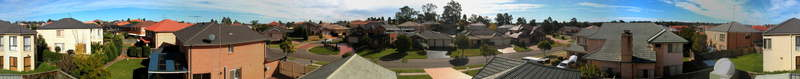
\includegraphics[scale=2.2]{landscape_beaumonthills.jpg}
%\caption{Figure caption}
\end{figure}

This is the only way to get a high resolution panorama and although this
procedure is based on the Microsoft Windows System the basics will apply
to any platform that can run the programs mentioned or similar programs
on the preferred system. If you want a high resolution this is the only
method to use. The first thing needed for a personalised landscape to
superimpose on the horizon display is a 360$\degree$ panorama with a transparent
background. To make this you will need the following:

\begin{itemize}
\item
  A digital camera on a tripod or stable platform
\item
  A program to convert the pictures into a 360$\degree$ panorama
\item
  A program to remove the background and convert the panorama into about
  8 square pictures in PNG format for insertion into Stellarium as the
  sides and if possible a similar square picture of the base you are
  standing on to form the ground. This last requirement is only really
  possible if this area is relatively featureless as the problem of
  knitting a complex base is well nigh impossible.
\item
  Patience. (Maybe a soundproof room so that the swearing wont be heard
  when you press the wrong key and lose an hours work)
\end{itemize}

\subsection{The Camera}\label{the-camera}

Digital cameras are easy and cheaply available these days so whatever
you have should do. One mega-pixel resolution is quite sufficient.

The camera needs to be mounted on a tripod so that reasonably orientated
pictures can be taken. Select a time of day that is quite bright with a
neutral cloudy sky so there will be no shadows and a sky of the same
overall texture. This will make it easier to remove later. The pictures
were all saved in the JPG format which was used as the common format for
all processes up to the removal of the background.

With a camera that takes 4:3 ratio pictures I found 14 evenly spaced
pictures gave the best 360$\degree$ panorama in the program I used to produce
it.

\subsection{Processing into a
Panorama}\label{processing-into-a-panorama}

This is the most complicated part of the process of generating the
panorama. I used two separate programs to do this. Firstly I used The
Gimp to re size the panels to 1024x768 and so make them easier to handle
in the panorama program.

When I had my 14 processed pictures I inserted them into the panorama
program. I first used a program called the Panorama Factory. Version 1.6
is a freebee that works well and can be downloaded from the internet - a
Google search will find it. I later used version 3.4 that is better and
cost about \$40 off the Internet. This program has many options and can
be configured to suit most cameras and can make a seamless 360$\degree$ panorama
in barrel form that will take a highly trained eye to find where the
joins occur.

The resulting panorama was then loaded into The Gimp and trimmed to a
suitable size. Mine ended up 14024 x 1601 pixels. I trimmed the vertical
size to 1024 by cutting back then stretched the 14024 to 14336 pixels,
with almost no distortion, that would allow cutting into 14 1024 x1024
pictures at a later date. If the height of the panorama had been greater
I could have made fewer pictures and so shown more of the foreground.
See figure {[}fig:panorama360{]}.

If you have prominent foreground items like posts wires etc. that occur
in adjacent pictures the panorama program will have difficulty in
discerning them because of the 3D effect and may give double images. I
overcame this by painting out the offending item by cut and paste
between the two pictures. Quite easy with a little practice using the
zoom in facility and I found the MSpaint program the easiest to do this
in.

\begin{figure}[h]
\centering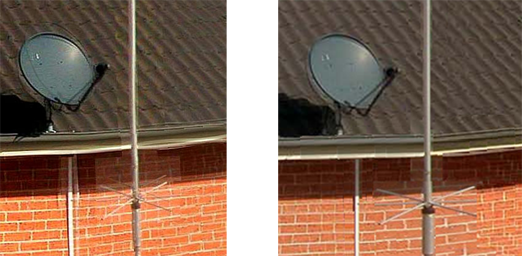
\includegraphics[scale=2.0]{BEAU-3c}
%\caption{Figure caption}
\end{figure}

\subsection{Removing the background to make it
transparent}\label{removing-the-background-to-make-it-transparent}

This is the most complex part of the process and requires a program that
can produce transparency to parts of your picture, commonly called an
alpha channel. Two programs I know of will do this. The very expensive
and sophisticated Adobe Photoshop and a freebee called The Gimp. I used
photoshop to cut the full panorama into 1024 x 1024 textures because it
was the easiest to do accurate cutting but it can be done in TheGimp as
well.

I first used Photoshop to produce the alpha channel because it was the
only way I knew but I now use the GIMP as it is much easier to process
the individual textures than removing the background from the full
panorama.

\begin{enumerate}
\item
  Load the 1st section into TheGimp
\item
  Next create a new empty picture 1024 x 1024 then use the advanced tab
  to make the background color transparency. Copy the original texture
  onto this new picture base so that it exactly fits the frame then
  select layer from the menu and press anchor. This will create a new
  picture with with an alpha channel. By using the select by color and
  lasso etc cut out the parts you don't want this will expose the
  checkerboard background. When you are happy with the removal save the
  texture in *.png format to preserve the alpha layer.
\item
  Do the same with the remaining pictures to make all the components of
  the landscape.
\item
  Make a new directory for the landscape. This should be a sub-directory
  of either the /landscapes or /landscapes directory. The name of the
  directory should be unique to your landscape, and is the landscape ID.
  The convention is to use a single descriptive word in lowercase text,
  for example gueriens. Place your pictures your new directory.
\item
  In your new landscape directory, create a new file called
  landscape.ini file (I used wordpad). Add a line for the
  {[}landscape{]} section. It's probably easiest to copy the
  landscape.ini file for the Gueriens landscape and edit it. Edit the
  name Guereins in every instance to the name you have given your
  landscape. Don't forget to make the number of tex entries agree with
  the number of your pictures. If you haven't made a groundtex picture
  use one of the existing ones from the file or make a square blank
  picture of your own idea. Because I took my pictures from the roof of
  the house I used an edited picture of the roof of my house from Google
  Earth. It was pretty cruddy low resolution but served the purpose.
\item
  Next you need to orientate your picture North with true North. This is
  done roughly by making the arrangement of side1 to siden suit your
  site as close as possible. Now you need to edit the value of
  decor\_angle\_rotatez to move your landscape in azimuth. Edit
  decor\_alt\_angle to move you landscape in altitude to align your
  visible horizon angle. Edit ground\_angle\_rotatez to align your
  ground with the rest of the landscape. Leave the other entries they
  are suitable as is.
\end{enumerate}

After re-starting Stellarium, your landscape will appear in the
landscape folder of the main menu , and can be selected as required.

\section{Making a Spherical
Panorama}\label{making-a-spherical-panorama}

A simpler method of making a panorama is to use the spherical method.
These can be made to create the full panorama using the program
Autostitch. The big advantage of the spherical panorama is that it does
not need a ground panel. However the drawback with the Spherical
panorama is that few computer video cards will reproduce a panorama
larger than 4096 x 2048 pixels and many will not do better than 2048 x
1024 pixels

\begin{figure}[h]
\centering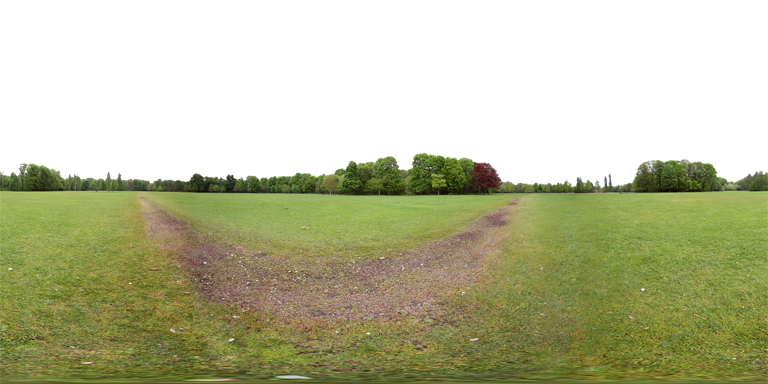
\includegraphics{egarden}
%\caption{Figure caption}
\end{figure}

The Autostitch program is quite easy to use. Make sure your panorama
shots take the ground almost up to your feet and follow the instructions
in the readme file. \href{http://www.example.com}{link title} When the
panorama is finished it will be in *,jpg format. This will need to be
converted to a *.png with transparent background (alpha layer) and have
the sky removed. This can be done in TheGimp as in the multi-panel type.
When the sky is removed make sure you save the landscape in *.png
format.

My computer will only do 2048 by 1024, If I try to load a larger type I
just get a white screen. With this problem I used the following
procedure to make the spherical into a four panel multi-panel landscape
with a very effective ground that matched well

\subsection{Converting a Spherical Panorama into a Multi
Panel}\label{converting-a-spherical-panorama-into-a-multi-panel}

Most computers with standard video cards will not display spherical
panoramas larger than 4096 x 2048 and some will not even go beyond 2048
x 1024. This makes rather poor resolution panaoramas. OK for planets but
not very pretty for your local environment. If the panorama can have a
horizontal section cut out that can keep the detail within a 1024
vertical boundary it is ideal for processing into 1024 x 1024 sections.
When you have the sections proceed as with the previous description

\begin{figure}[h]
\centering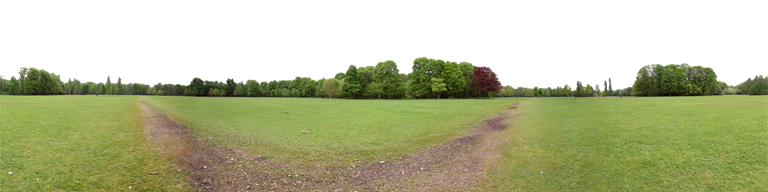
\includegraphics{egarden-narrow}
%\caption{Figure caption}
\end{figure}

I made the egarden into a 4096 x 1024 quite easily because there was a
lot of blank space above the horizon. This would allow 4 panels 1024 x
1024 pixels.in fact if I had a 8192 x 4096 panorama I could have made it
into 8 1024 x 1024 panels. This would have given me quite a high
resolution horizon

\begin{figure}[h]
\centering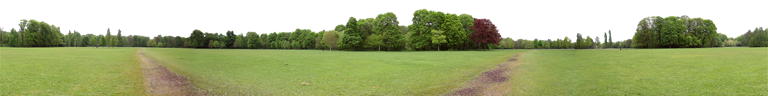
\includegraphics{egarden-narrow-2}
%\caption{Figure caption}
\end{figure}


\begin{enumerate}
\item
  Load the sections into TheGimp and process them into 1024 x 1024
  textures with alpha layers as before.
\item
  Next use a 2048 x 1024 version of the panorama in Stellarium. Drag the
  screen around so it produces a centralised picture on the Stellarium
  screen of the ground at the highest resolution possible and take a
  screen shot. This screen shot can be then processed into a quite
  effective ground texture in TheGimp that can be adjusted to match the
  rest of the panorama.
  \begin{figure}[h]
  \centering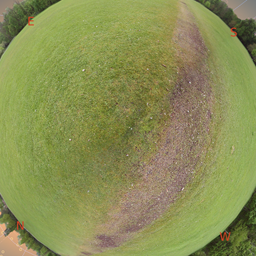
\includegraphics[scale=2.0]{egardembase}
  %\caption{Figure caption}
  \end{figure}
\item
  Make a new directory etc. for the landscape.
\item
  You can make it fit using the variablein the landscape.ini file
  decor\_alt\_angle=xx decor\_angle\_shift=xx and
  decor\_angle\_rotatez=xx.Then the ground can be matched with
  ground\_angle\_shift=xx and ground\_angle\_rotatez=xx.
\item
  Make sure the draw\_ground\_first=1 to ensure that the main panorama
  overplays the ground
\end{enumerate}

After re-starting Stellarium, your landscape will appear in the
landscape tab of the main menu, and can be selected as required.

When the panorama is finished it will be in *.jpg format. It will need
to be converted to a *.png with transparent background (alpha layer) and
have the sky removed. This is done in TheGimp as in the multipanel type.
When the sky is removed make sure you save the landscape in *.png
format.

The drawback with the spherical panorama is that few computer video
cards will reproduce a panorama larger than 4096 x 2048 pixels in
Stellarium and many will not do better than 2048 x 1024 pixels.

My computer will only do 2048 by 1024, If I try to load a larger type I
just get a white screen. With this problem I used the following
procedure to make the spherical into a four panel multi panel landscape
with a very effective ground that matched well.

\section{Making a Fish eye
Panorama}\label{making-a-fish-eye-panorama}

This sort of panorama needs a very expensive fisheye lens on your
camera. It is really only practical for a planetarium display to give a
simple more or less silouette landscape where the ground is completely
obscured. It can only be used with quite small pictures of no more than
1024 x 1024 pixels. Once you have your fisheye texture it must still be
processed in TheGimp to remove the sky and convert into an alpha layer
texture

\begin{figure}[h]
\centering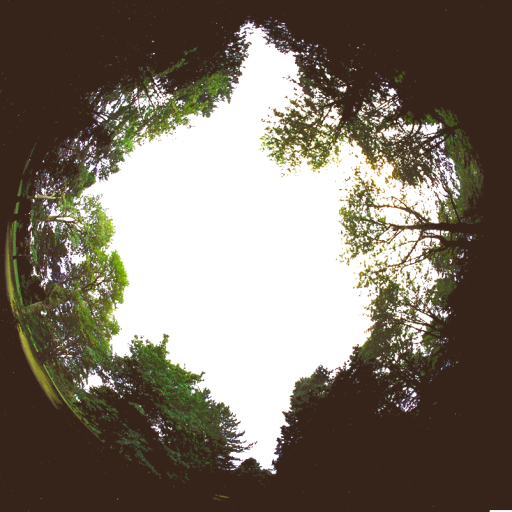
\includegraphics[scale=3.0]{trees_512}
%\caption{Figure caption}
\end{figure}

The sample supplied with Stellarium is called trees. The horizon needs
to be identified and the picture sized so that the panorama above the
horizon is sited to be about 80\% of the total extent and the the
balance of the border filled with a dark colour right up to the horizon.
This will make the horizon in your landscape at 0 degrees.

It is possible to make a synthetic fisheye texture using the same method
as making a ground from a spherical panorama but it is hardly worth the
trouble as even a simple 2048 x 1024 pixel sperical will give a far
better result.

\chapter{Deep-Sky Objects}\label{deep-sky-objects}

Extended objects are those which are external to the solar system, and
are not point-sources like stars. Extended objects include galaxies,
planetary nebulae and star clusters. These objects may or may not have
images associated with them. Stellarium also comes with a catalogue with
over 14,000 extended objects containing the combined data from many
catalogues, with 190 images.

Since to version 0.10.0 Stellarium uses new method of displaying
textures using the ``json'' cataloguing system. At the same time the
Simbad online catalogue was added to the search feature making it
largely redundant and used now only as a first search point or if there
is no internet connection.

If the object has a name (not just a catalogue number), you should add
one or more records to the \texttt{.../nebulae/default/names.dat} file
(where \texttt{...} is either the installation directory or the user
directory). See section
\emph{\protect\hyperlink{Modifyingux5fnames.dat}{Modifying names.dat}}
for details of the file format.

If you wish to associate a texture (image) with the object, you must now
add a record to the \texttt{.../nebulae/default/textures.json} file. See
section \emph{\protect\hyperlink{Modifyingux5ftextures.json}{Modifying
textures.json}} for details of the file format.

Nebula images should have dimensions which are integer powers of two,
i.e. 1, 2, 4, 8, 16, 32, 64, 128, 256, 512, 1024 ... pixels along each
side. If this requirement is not met, your textures may not be visible,
or graphics performance may be seriously impacted. PNG or JPG formats
are both supported.

\section{GUI for manage by Deep-Sky
Objects}\label{gui-for-manage-by-deep-sky-objects}

\begin{figure}[h]
\centering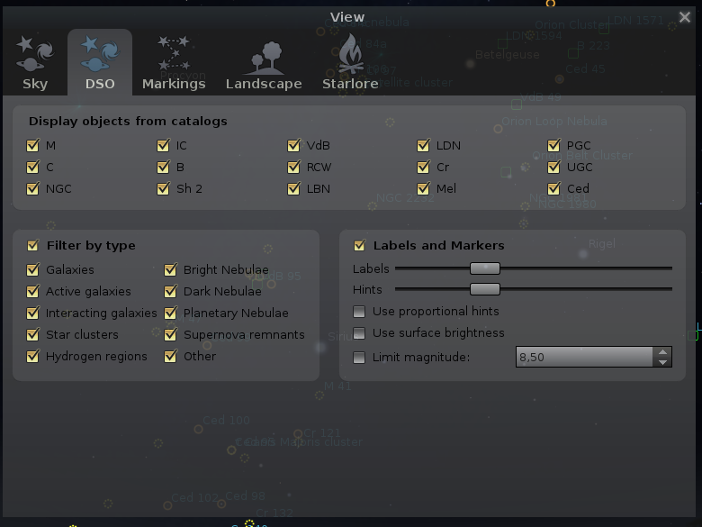
\includegraphics{DSO_GUI}
%\caption{Figure caption}
\end{figure}

\section{Stellarium DSO Catalog}\label{stellarium-dso-catalog}

Stellarium DSO Catalog is contains over 1400 objects and he available
for end users as collection of files:

\begin{itemize}
\item
  \texttt{catalog.txt} - Stellarium DSO Catalog in ASCII format for
  editing data;
\item
  \texttt{catalog.dat} - Stellarium DSO Catalog in binary format for
  usage within Stellarium;
\item
  \texttt{names.dat} - list of proper names of the objects from
  \texttt{catalog.dat} file.
\end{itemize}

ASCII file can be converted into binary format through enabling option
\texttt{devel/convert\_dso\_catalog\ =\ true} in the \texttt{config.ini}
file. The file \texttt{catalog.txt} should be put to the directory
\texttt{.../nebulae/default/}.

Stellarium DSO Catalog contains data and supported the designations for
follow catalogues:

\begin{itemize}
\item
  New General Catalogue (NGC)
\item
  Index Catalogue (IC)
\item
  Messier Catalog (M)
\item
  Caldwell Catalogue (C)
\item
  Barnard Catalogue (B)
\item
  Sharpless Catalogue (Sh2)
\item
  Van den Bergh Catalogue of reflection nebulae (VdB)
\item
  A catalogue of H$\alpha$-emission regions in the southern Milky Way (RCW)
\item
  Lynds' Catalogue of Dark Nebulae (LDN)
\item
  Lynds' Catalogue of Bright Nebulae (LBN)
\item
  Collinder Catalogue (Cr)
\item
  Melotte Catalogue of Deep Sky Objects (Mel)
\item
  HYPERLEDA. I. Catalog of galaxies (PGC)\footnote{Partial support}
\item
  The Uppsala General Catalogue of Galaxies (UGC)\footnote{Partial
    support}
\item
  Cederblad Catalog of bright diffuse Galactic nebulae (Ced)
\end{itemize}

\section{Modifying catalog.dat}\label{modifying-catalog.dat}

This section is described inner structure of files \texttt{catalog.dat}
(has binary format) and \texttt{catalog.txt} (has ASCII format).
Stellarium can convert ASCII file into the binary format file for usage
within planetarium.

Each line contains one record, each record consisting of the following
fields with \emph{tab} char as delimiter:

\begin{longtabu} to \textwidth {l|l|X}
\toprule
\emph{Column} & \emph{Type} & \emph{Description}\tabularnewline
\midrule
1 & integer & Deep-Sky Object Identificator\tabularnewline
2 & float & RA (decimal degrees)\tabularnewline
3 & float & Dec (decimal degrees)\tabularnewline
4 & float & B magnitude\tabularnewline
5 & float & V magnitude\tabularnewline
6 & string & Object type (Possible values see in table
\emph{\protect\hyperlink{Typesux5fofux5fObjects}{Types of
Objects}}).\tabularnewline
7 & string & Morphological type of object\tabularnewline
8 & float & Major axis size or radius (arcmin)\tabularnewline
9 & float & Minor axis size (arcmin)\tabularnewline
10 & integer & Orientation angle (degrees)\tabularnewline
11 & float & Redshift\tabularnewline
12 & float & Error of redshift\tabularnewline
13 & float & Parallax (mas)\tabularnewline
14 & float & Error of parallax (mas)\tabularnewline
15 & float & Non-redshift distance (Mpc for galaxies, kpc for other
objects)\tabularnewline
16 & float & Error of non-redsift distance (Mpc for galaxies, kpc for
other objects)\tabularnewline
17 & integer & NGC number (New General Catalogue)\tabularnewline
18 & integer & IC number (Index Catalogue)\tabularnewline
19 & integer & M number (Messier Catalog)\tabularnewline
20 & integer & C number (Caldwell Catalogue)\tabularnewline
21 & integer & B number (Barnard Catalogue)\tabularnewline
22 & integer & Sh2 number (Sharpless Catalogue)\tabularnewline
23 & integer & VdB number (Van den Bergh Catalogue of reflection
nebulae)\tabularnewline
24 & integer & RCW number (A catalogue of H$\alpha$-emission regions in the
southern Milky Way)\tabularnewline
25 & integer & LDN number (Lynds' Catalogue of Dark
Nebulae)\tabularnewline
26 & integer & LBN number (Lynds' Catalogue of Bright
Nebulae)\tabularnewline
27 & integer & Cr number (Collinder Catalogue)\tabularnewline
28 & integer & Mel number (Melotte Catalogue of Deep Sky
Objects)\tabularnewline
29 & integer & PGC number (HYPERLEDA. I. Catalog of galaxies);
partial\tabularnewline
30 & integer & UGC number (The Uppsala General Catalogue of Galaxies);
partial\tabularnewline
31 & string & Ced number (Cederblad Catalog of bright diffuse Galactic
nebulae)\tabularnewline
\bottomrule
\end{longtabu}

\subsection{Types of Objects}\label{types-of-objects}

Possible values for type of objects in the file \texttt{catalog.dat}.

\begin{longtabu} to \textwidth {l|X}
\toprule
\emph{Type} & \emph{Description}\tabularnewline
\midrule
G & Galaxy\tabularnewline
GX & Galaxy\tabularnewline
AGX & Active Galaxy\tabularnewline
RG & Radio Galaxy\tabularnewline
IG & Interacting Galaxy\tabularnewline
GC & Globular Cluster\tabularnewline
OC & Open Cluster\tabularnewline
NB & Nebula\tabularnewline
PN & Planetary Nebula\tabularnewline
DN & Dark Nebula\tabularnewline
RN & Reflection Nebula\tabularnewline
C+N & Cluster associated with nebulosity\tabularnewline
HII & HII Region\tabularnewline
SNR & Supernova Remnant\tabularnewline
BN & Bipolar Nebula\tabularnewline
EN & Emission Nebula\tabularnewline
SA & Stellar Association\tabularnewline
SC & Star Cloud\tabularnewline
CL & Cluster\tabularnewline
IR & Infra-Red Object\tabularnewline
QSO & Quasar\tabularnewline
Q? & Possible Quasar\tabularnewline
ISM & Interstellar Matter\tabularnewline
EMO & Emission Object\tabularnewline
LIN & LINEAR-type Active Galaxies\tabularnewline
BLL & BL Lac Object\tabularnewline
BLA & Blazar\tabularnewline
MOC & Molecular Cloud\tabularnewline
YSO & Young Stellar Object\tabularnewline
PN? & Possible Planetary Nebula\tabularnewline
PPN & Protoplanetary Nebula\tabularnewline
$\ast$ & Star\tabularnewline
$\ast\ast$ & Double Star\tabularnewline
MUL & Multiple Star\tabularnewline
\emph{empty} & Unknown type, catalog errors, \emph{Unidentified Southern
Objects} etc.\tabularnewline
\bottomrule
\end{longtabu}

\section{Modifying names.dat}\label{modifying-names.dat}

Each line in the \texttt{names.dat} file contains one record. A record
relates an extended object catalogue number (from \texttt{catalog.dat})
with a name. A single catalogue number may have more than one record in
this file.

The record structure is as follows:

\begin{longtabu} to \textwidth {l|l|l|X}
\toprule
\emph{Offset} & \emph{Length} & \emph{Type} & \emph{Description}\tabularnewline
\midrule
0 & 5 & \%5s & Designator for catalogue (prefix)\tabularnewline
5 & 15 & \%d & Identificator for object in the catalog\tabularnewline
20 & 60 & \%s & Proper name of the object (translatable)\tabularnewline
\bottomrule
\end{longtabu}

If an object has more than one record in the \texttt{names.dat} file,
the last record in the file will be used for the nebula label.

\section{Modifying textures.json}\label{modifying-textures.json}

This file is used to describe each nebula image. The file structure
follows the JSON format, a detailed description of which may be found at
. The textures.json file which ships with Stellarium has the following
structure:

\begin{itemize}
\item
  serverCredits (optional) - a structure containing the following
  key/value pairs:

  \begin{itemize}
  \item
    short - a short identifier of a server where the json file is found,
    e.g. ``ESO''
  \item
    full - a longer description of a server, e.g. ``ESO Online Digitised
    Sky Survey Server''
  \item
    infoURL - a URL pointing at a page with information about the server
  \end{itemize}
\item
  imageCredits - a structure containing the same parts as a
  serverCredits structure but referring to the image data itself
\item
  shortName - an identifier for the set of images, to be used inside
  Stellarium
\item
  minResolution - minimum resolution, applies to all images in the set,
  unless otherwise specified at the image level
\item
  maxBrightness - the maximum brightness of an image, applies to all
  images in the set, unless otherwise specified at the image level
\item
  subTiles - a list of structures describing indiviual image tiles, or
  referring to another json file. Each subTile may contain:

  \begin{itemize}
  \item
    minResolution
  \item
    maxBrightness
  \item
    worldCoords
  \item
    subTiles
  \item
    imageCredits
  \item
    imageUrl
  \item
    textureCoords
  \end{itemize}
\item
  shortName (name for the whole set of images, e.g. ``Nebulae'')
\item
  miniResolution (applies to all images in set)
\item
  alphaBlend (applies to all images in set)
\item
  subTiles list of images. Each image record has the following
  properties:

  \begin{itemize}
  \item
    imageCredits (itself a list of key/pairs)
  \item
    imageUrl (e.g. file name)
  \item
    worldCoords (a list of four pairs of coordinates representing the
    corners of the image)
  \item
    textureCoords (a list of four pairs of corner descriptions. i.e.
    which is top left of image etc)
  \item
    minResolution (over-rides file-level setting)
  \item
    maxBrightness
  \end{itemize}
\end{itemize}

Items enclosed in Quotation marks are strings for use in the program.
Syntax is extremely important. Look at the file with a text editor to
see the format. Items in \textless{}\textgreater{} are user provided
strings and values to suit the texture and source.

\texttt{Line~1~“imageCredits”:~\{“short”~:~“}\texttt{”~:~“infoUrl”:~}\href{http://}{\texttt{http://}}\texttt{\},~}\\
\texttt{Line~2~“imageUrl”~:~“}\texttt{”,~}\\
\texttt{Line~3~“worldCoords”~:~\textless{}~decimal~numerical~values~of~the~J2000~coordinates~of~the~corners~of~the~texture~\textgreater{}~These~values~displayed~to~4~decimal~places~in~the~format~of~the~texture~coordinates~}\\
\texttt{Line~4~“textureCoords”~:~{[}{[}{[}~0,0{]},{[}1,0{]},{[}1,1{]},{[}0,1{]}{]}{]},~Where~0,0~is~South~Left~,~1,0~the~South~Right~,~1,1~North~Right~,~0,1~North~Left~corners~of~texture~Format~=~RA~in~degrees,~Dec~in~degrees~}\\
\texttt{Line~5~“MinResolution”~:~}\texttt{,~}\\
\texttt{Line~6~“maxBrightness”~:~\textless{}~a~numerical~vale~representing~the~absolute~brightness~for~the~display\textgreater{}~}

Calculating of the coords of the corners of the images (plate solving)is
a time consuming project and needs to be fine tuned from the screen
display. As most images will be two dimensional, display on a spherical
display will limit the size to about 1 degree before distortion becomes
evident. Larger displays can be sectioned into a mosaic of smaller
textures for a more accurate display

\section{Adding Extra Nebulae
Images}\label{adding-extra-nebulae-images}

\subsection{\texorpdfstring{Preparing a photo for inclusion to the
\texttt{textures.json}
file}{Preparing a photo for inclusion to the textures.json file}}\label{preparing-a-photo-for-inclusion-to-the-textures.json-file}

\begin{figure}[h]
\centering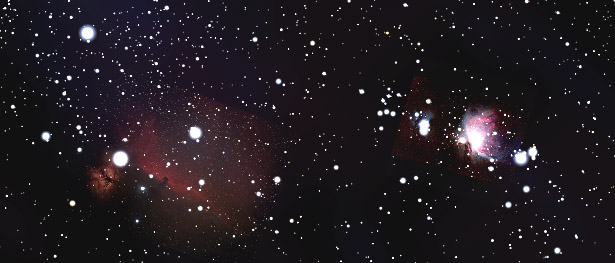
\includegraphics{nebula-display}
\caption{Screen shot of nebula images displayed in Stellarium}
\end{figure}

The first step is to take a photo of the object you wish to display in
Stellarium as a screen backdrop. Then when you have the picture you will
need align it so that north is directly up and not inverted side to side
or up and down as can happen with photos taken with a diagonal mirror in
the path. Next you will need to crop the picture, setting the main
feature at the centre and making the cropped size a factor of 2n eg. 64,
128, 256, 512 or 1024 pixels square. When cropping make sure you leave
at least five prominent background stars

The next step is to process your photo to make the background
black,black. This will ensure that your background will meld with the
Stellarium background and not be noticed. Suitable programs to do all
this are The Gimp (free in keeping with the Stellarium spirit) or
Photoshop if you can afford it.

When you have your prepared image you will need to plate solve it using
at least 6 known GSC stars that can be identified. That is why the
cropping with plenty of stars was necessary. When the plate is solved
you will need to find the J2000 coordinates of the corners and convert
them to decimal values to form the world coordinates in the
\texttt{textures.json} file.

\begin{figure}[h]
\centering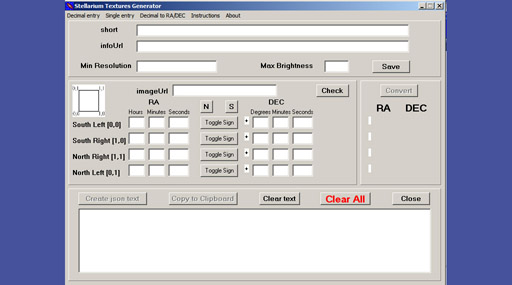
\includegraphics{EQ-Decimal.jpg}
\caption{A program to convert Equatorial coordinates into decimal
form and write a \texttt{textures.json} insert}
\end{figure}

The program in the picture can accept the corner coordinates of a
texture in your plate solving program into decimal values and write an
insert for the \texttt{textures.json} file. It is available as a freebee
from
\url{http://www.madpc.co.uk/~peterv/astroplover/equipnbits/Stellariumtextures.zip}

\begin{figure}[h]
\centering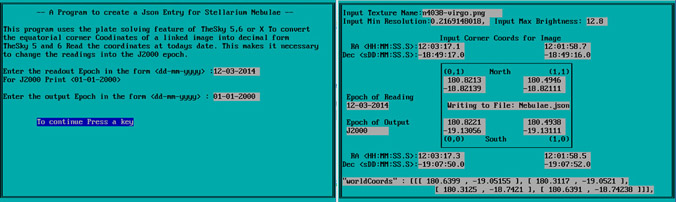
\includegraphics{pix-4.jpg}
\end{figure}

Here is a second program written in Qb64(gl)that will perform the same
task but allow manipulation of the epochs.
\url{http://barry.sarcasmogerdes.com/stellarium/uploads/writejsoninsert.zip}

\subsection{Plate Solving}\label{plate-solving}

Suitable programs that can accept your picture and calculate its corner
coordinates are hard to find. I have only found one that suits our
purpose and it is another expensive planetarium program, TheSkyX Pro.
However the older versions TheSky5 and 6 Pro will also do the job if
suitably configured although I could not solve the test program with the
TheSky6 that uses the same procedure as TheSky5 .

These programs have a link feature that can match your photo to the
selected area of the screen and superimpose it on the display with a box
around your photo provided it can match at least 6 stars from the GSC
that is included with the program. When this is fitted you can read the
corner coordinates of your texture in the Status bar by selecting them
with a mouse. TheSkyX can read these coordinates in J2000 values and
uses textures in the fits format but the earlier programs only read the
coordinates of the current program date. To read the J2000 coordinates
it is necessary to re start the program with the date set to 1-1-2000

To add the picture to TheSky5 you need first make a mono 8 bit version
of the photo and place it on the clipboard. Run TheSky and centre on the
object centre. Look in the Tools menu for the image link and select
setup. Tick show image frame to put a frame around the image.

Paste the clipboard image on the display and use the zoom and position
controls to get it as close to the size and position as possible by
visually matching stars. Go to the menu again and click on link wizard.
If you have been successful the window will show the number of stars
matched and the option to accept or continue. Accept and you will now
see all the matched stars have overlaid the picture. You can now read
off the corner coordinates from the status bar starting at the bottom
(south) left and continuing counter clockwise to the top (north) left.

\subsection{\texorpdfstring{Processing into a \texttt{textures.json}
insert}{Processing into a textures.json insert}}\label{processing-into-a-textures.json-insert}

Place your image in the \texttt{*.png} format in the
\texttt{.../nebulae/default/} folder. Ensure that the name matches the
\texttt{textures.json} entry.

Once you have the corner coordinates of your photo you can add them to
the decimal converter program and it will write an insert
\texttt{nebula.json} as a text file that you can paste directly into the
\texttt{textures.json} file that is in the \texttt{.../nebulae/default/}
folder.

Save the \texttt{textures.json} file with the new insert and run
Stellarium. Select the object in the Object selection window and slew to
it. Your image should be there and with a bit of luck it will nicely
overlay the stars in the Stellarium program. However this only rarely
happens so a little bit of tweaking of the json worldcoords will be
needed to get a perfect match. Select the telescope (equatorial mode).
This will show the area with north up. Select each corner in sequence
and make small changes to the coordinates. Re start Stellarium each time
and check if you have moved the right direction. Continue with each
corner until all the stars match. With a little bit of practice this
will be done in about 10 minutes.




\chapter{Landscapes}\label{customising-landscapes}
\label{ch:landscapes}

Stellarium comes with a selection of panorama landscapes which try to
link the sky with the observer's surrounding and thus create a more
immersive feeling.  It is possible to create your own landscapes for
Stellarium, this is described in
section~\ref{sec:landscapes:customizing}. 

\section{Landscape Types}
\label{sec:landscapes:types}


There are four types of landscape:

\begin{itemize}
\item
  \textbf{Polygonal Method} Using a text file with azimuths/altitudes.
\item
  \textbf{Single Fish-eye Method} Using a fish-eye panorama image.
\item
  \textbf{Single Spherical Method} Using a spherical panorama image.
\item
  \textbf{Multiple Image Method} (\textbf{also called ``old style''
  landscapes}) Using a series of images split from a 360$\degree$ ``strip''
  panorama image + a ground image.
\end{itemize}

Each landscape has its own sub-directory in
\texttt{\textless{}user\ directory\textgreater{}/landscapes} or
\texttt{\textless{}installation\ directory\textgreater{}/landscapes}.
The name of the sub-directory is called the \emph{landscape ID}. The
sub-directory must contain a file called \texttt{landscape.ini} which
describes the landscape type, texture filenames and other data. Texture
files for a landscape should by put in the same directory as the
\texttt{landscape.ini} file, although if they are not found there they
will be searched for in the \texttt{.../textures} directory, allowing
shared files for common textures such as the generic fog texture.

For example, the \emph{Moon} landscape that is provided with Stellarium
has the following files:

\texttt{.../landscapes/moon/landscape.ini}\\
\texttt{.../landscapes/moon/apollo17.png}

The \texttt{landscape.ini} file must contain a section called
\texttt{{[}landscape{]}}, which contains the details necessary to render
the landscape (which vary, depending on the type of the landscape).

There is also an optional \texttt{{[}location{]}} section which is used
to tell Stellarium where the landscape is in the solar system. If the
\texttt{{[}location{]}} section exists, Stellarium can automatically
adjust the location and observing conditions of the observer to match
the landscape.

\subsection{Polygonal Landscape}\label{polygonal-line-method}

This is the technically simplest of the landscapes, but may be used to
describe accurately measured horizon lines. The file that encodes
horizon altitudes can also be used in all other landscape types. If
present there, it will be used to define object visibility (instead of
the opacity of the landscape photo textures) and, if
\texttt{horizon\_line\_color} is defined, will be plotted.

There is a small caveat: Sometimes, there may appear vertical lines from
some corners towards the zenith or the mathematical horizon, e.g. if
there is a vertex including azimuth 0 or 180. If this irritates you,
just offset this azimuth minimally (e.g., 180.00001).

The \texttt{landscape.ini} file for a polygonal type landscape looks
like this (this example is based on the Geneve landscape which was
borrowed from Cartes du Ciel and comes with Stellarium):

\begin{config}
\texttt{{[}landscape{]}}\\
\texttt{name~=~Geneve}\\
\texttt{type~=~polygonal}\\
\texttt{author~=~Georg~Zotti;~Horizon~definition~by~Patrick~Chevalley}\\
\texttt{description~=~Horizon~line~of~Geneve.~Demonstrates~compatibility~with~horizon~descriptions~from~~Cartes~du~Ciel.}\\
\texttt{polygonal\_horizon\_list~=~horizon\_Geneve.txt}\\
\texttt{polygonal\_angle\_rotatez~=~0}\\
\texttt{ground\_color~=~.15,.45,.45}\\
\texttt{horizon\_line\_color~=~~.75,.45,.45}
\end{config}

Where:

\begin{itemize}
\item
  \textbf{name} is what appears in the landscape tab of the
  configuration window.
\item
  \textbf{type} identifies the method used for this landscape.
  ``polygonal'' in this case.
\item
  \textbf{author} lists the author(s) responsible for images and
  composition.
\item
  \textbf{description} gives a short description visible in the
  selection panel. The text will be superseded by optional
  \texttt{description.\&lt;lang\&gt;.utf8} files.
\item
  \textbf{polygonal\_horizon\_list} is the name of the horizon data file
  for this landscape.
\item
  \textbf{polygonal\_horizon\_list\_mode} (optional) the two first
  columns in the list are numbers: azimuth and altitude or zenith
  distance, in either degrees or radians or gradians(gon). The value
  must be one of
  \texttt{azDeg\_altDeg\textbar{}azDeg\_zdDeg\textbar{}azRad\_altRad\textbar{}azRad\_zdRad\textbar{}azGrad\_altGrad\textbar{}azGrad\_zdGrad}.
  Default: azDeg\_altDeg
\item
  \textbf{polygonal\_angle\_rotatez} (optional, default=0) Angle
  (degrees) to adjust azimuth. This may be used to apply a (usually)
  small offset rotation, e.g. when you have measured the horizon in a
  grid-based coordinate system like UTM and have to compensate for the
  meridian convergence.
\item
  \textbf{ground\_color} (optional, default=``0,0,0'', i.e., black)
  Color for the area below the horizon line. Each R,G,B component is a
  float within 0..1.
\item
  \textbf{horizon\_line\_color} (optional, default: invisible) used to
  draw a polygonal horizon line. Each R,G,B component is a float within
  0..1.
\item
  \textbf{minimal\_brightness} (optional, default=-1, i.e. use preset
  landscape/minimal\_brightness from global \texttt{config.ini}) Some
  minimum brightness to keep landscape visible.
\item
  \textbf{minimal\_altitude} (optional, default=-2) Some sky elements,
  e.g. stars, are not drawn below this altitude. Under certain
  circumstances you may want to specify something else here. (since
  V0.14)
\end{itemize}

\subsection{Single Fish-eye Landscape}\label{single-fish-eye-method}

The \emph{Trees} landscape that is provided with Stellarium is an
example of the single fish-eye method, and provides a good illustration.
The centre of the image is the spot directly above the observer (the
zenith). The point below the observer (the nadir) becomes a circle that
just touches the edges of the image. The remaining areas of the image
(the corners outside the circle) are not used.

The image file should be saved in PNG format with alpha transparency.
Wherever the image is transparent is where Stellarium will render the
sky.

The \texttt{landscape.ini} file for a fish-eye type landscape looks like
this (this example is based on the Trees landscape which comes with
Stellarium):

\begin{config}
\texttt{{[}landscape{]}}\\
\texttt{name~=~Trees}\\
\texttt{type~=~fisheye}\\
\texttt{author~=~Robert~Spearman.~Light~pollution~image:~Georg~Zotti}\\
\texttt{description~=~Trees~in~Greenlake~Park,~Seattle}\\
\texttt{maptex~=~trees\_512.png}\\
\texttt{maptex\_illum~=~trees\_illum\_512.png}\\
\texttt{maptex\_fog~=~trees\_fog\_512.png}\\
\texttt{texturefov~=~210}\\
\texttt{angle\_rotatez~=~17}\\
\texttt{tesselate\_rows~=~28}\\
\texttt{tesselate\_cols~=~60}
\end{config}

Where:

\begin{itemize}
\item
  \textbf{name} is what appears in the landscape tab of the
  configuration window.
\item
  \textbf{type} identifies the method used for this landscape.
  ``fisheye'' in this case.
\item
  \textbf{author} lists the author(s) responsible for images and
  composition.
\item
  \textbf{description} gives a short description visible in the
  selection panel. The text will be superseded by optional
  \texttt{description.\&lt;lang\&gt;.utf8} files.
\item
  \textbf{maptex} is the name of the image file for this landscape.
\item
  \textbf{maptex\_fog} (optional) is the name of the fog image file for
  this landscape.
\item
  \textbf{maptex\_illum} (optional) is the name of the nocturnal
  illumination/light pollution image file for this landscape.
\item
  \textbf{texturefov} is the field of view that the image covers in
  degrees.
\item
  \textbf{angle\_rotatez} (optional) Angle (degrees) to adjust azimuth.
\item
  \textbf{tesselate\_rows} (optional, default=20) If straight edges in
  your landscape appear broken, try increasing.
\item
  \textbf{tesselate\_cols} (optional, default=40) If straight edges in
  your landscape appear broken, try increasing.
\item
  \textbf{polygonal\_horizon\_list} (optional) is the name of the
  (measured) horizon data file for this landscape.
\item
  \textbf{polygonal\_horizon\_list\_mode} (optional) the two first
  columns in the list are numbers: azimuth and altitude or zenith
  distance, in either degrees or radians or gradians(gon). The value
  must be one of
  \texttt{azDeg\_altDeg \textbar{} azDeg\_zdDeg \textbar{} azRad\_altRad \textbar{} azRad\_zdRad \textbar{} azGrad\_altGrad \textbar{} azGrad\_zdGrad}.
  Default: \texttt{azDeg\_altDeg}
\item
  \textbf{polygonal\_angle\_rotatez} (optional, default=0) Angle
  (degrees) to adjust azimuth. This may be used to apply a (usually)
  small offset rotation, e.g. when you have measured the horizon in a
  grid-based coordinate system like UTM and have to compensate for the
  meridian convergence.
\item
  \textbf{horizon\_line\_color} (optional, default: invisible) used to
  draw a polygonal horizon line.
\item
  \textbf{minimal\_brightness} (optional, default=-1, i.e. use preset
  landscape/minimal\_brightness from global \texttt{config.ini}) Some
  minimum brightness to keep landscape visible.
\item
  \textbf{minimal\_altitude} (optional, default=-2) Some sky elements,
  e.g. stars, are not drawn below this altitude. Under certain
  circumstances you may want to specify something else here. (since
  V0.14)
\end{itemize}

\subsection{Single Panorama Landscape}\label{single-panorama-method}

This method uses a more usual type of panorama - the kind which is
produced directly from software such as \emph{autostitch} or Hugin
(http://hugin.sourceforge.net/). The panorama file should be copied into
the
\texttt{\textless{}config\ root\textgreater{}/landscapes/\textless{}landscape\_id\textgreater{}}
directory, and a \texttt{landscape.ini} file created. The \emph{Moon}
landscape which comes with Stellarium provides a minimal example of the
contents of a landscape.ini file for a spherical type landscape:

\begin{config}
\texttt{{[}landscape{]}}\\
\texttt{name~=~Moon}\\
\texttt{type~=~spherical}\\
\texttt{maptex~=~apollo17.png}
\end{config}

A more elaborate example is found with the \emph{Grossmugl} landscape:

\begin{config}
\texttt{{[}landscape{]}}\\
\texttt{name~=~Grossmugl}\\
\texttt{type~=~spherical}\\
\texttt{author~=~Guenther~Wuchterl,~Kuffner-Sternwarte.at;~Lightscape:~Georg~Zotti}\\
\texttt{description~=~Field~near~Leeberg,~Grossmugl~(Riesentumulus),~Austria~-~Primary~Observing~Spot~of~the~Grossmugl~Starlight~Oasis~-~}\href{http://starlightoasis.org}{\texttt{http://starlightoasis.org}}\\
\texttt{maptex~=~grossmugl\_leeberg\_crop11.25.png}\\
\texttt{maptex\_top=11.25~}\\
\texttt{maptex\_fog~=~grossmugl\_leeberg\_fog\_crop22.5.png}\\
\texttt{maptex\_fog\_top~=~22.5}\\
\texttt{maptex\_fog\_bottom~=~-22.5}\\
\texttt{maptex\_illum~=~grossmugl\_leeberg\_illum\_crop0.png}\\
\texttt{maptex\_illum\_bottom~=~0}\\
\texttt{angle\_rotatez=-89.1}\\
\texttt{minimal\_brightness~=~0.0075}\\
\texttt{polygonal\_horizon\_list~=~horizon\_grossmugl.txt}\\
\texttt{polygonal\_angle\_rotatez=0}\\
\texttt{horizon\_line\_color~=~~.75,.45,.45}\\
\texttt{minimal\_altitude~=~-1}
\end{config}

Where:

\begin{itemize}
\item
  \textbf{name} is what appears in the landscape tab of the
  configuration window.
\item
  \textbf{type} identifies the method used for this landscape.
  ``spherical'' in this case.
\item
  \textbf{author} lists the author(s) responsible for images and
  composition.
\item
  \textbf{description} gives a short description visible in the
  selection panel. The text will be superseded by optional
  \texttt{description.\&lt;lang\&gt;.utf8} files.
\item
  \textbf{maptex} is the name of the image file for this landscape.
\item
  \textbf{maptex\_top} (optional; default=90) is the altitude angle of
  the top edge.
\item
  \textbf{maptex\_bottom} (optional; default=-90) is the altitude angle
  of the bottom edge. Usually you will not require this, or else there
  will be a hole at your feet. ;-)
\item
  \textbf{maptex\_fog} (optional; default: no fog) is the name of the
  fog image file for this landscape.
\item
  \textbf{maptex\_fog\_top} (optional; default=90) is the altitude angle
  of the top edge of the fog texture. Useful to crop away parts of the
  image to conserve texture memory.
\item
  \textbf{maptex\_fog\_bottom} (optional; default=-90) is the altitude
  angle of the bottom edge.
\item
  \textbf{maptex\_illum} (optional; default: no illumination layer) is
  the name of the nocturnal illumination/light pollution image file for
  this landscape.
\item
  \textbf{maptex\_illum\_top} (optional; default=90) is the altitude
  angle of the top edge, if you have light pollution only close to the
  horizon.
\item
  \textbf{maptex\_illum\_bottom} (optional; default=-90) is the altitude
  angle of the bottom edge.
\item
  \textbf{angle\_rotatez} (optional, default=0) Angle (degrees) to
  adjust azimuth. If 0, the left/right edge is due east.
\item
  \textbf{tesselate\_rows} (optional, default=20) If straight edges in
  your landscape appear broken, try increasing. This is the number of
  rows for the maptex. Fog and illumination textures will have a similar
  vertical angle.
\item
  \textbf{tesselate\_cols} (optional, default=40) If straight edges in
  your landscape appear broken, try increasing.
\item
  \textbf{polygonal\_horizon\_list} (optional) is the name of the
  (measured) horizon data file for this landscape. Can be used to query
  horizon transparency (for accurate object rising/setting times)
\item
  \textbf{polygonal\_horizon\_list\_mode} (optional) the two first
  columns in the list are numbers: azimuth and altitude or zenith
  distance, in either degrees or radians or gradians(gon). The value
  must be one of
  \texttt{azDeg\_altDeg\textbar{}azDeg\_zdDeg\textbar{}azRad\_altRad\textbar{}azRad\_zdRad\textbar{}azGrad\_altGrad\textbar{}azGrad\_zdGrad}.
  Default: \texttt{azDeg\_altDeg}
\item
  \textbf{polygonal\_angle\_rotatez} (optional, default=0) Angle
  (degrees) to adjust azimuth. This may be used to apply a (usually)
  small offset rotation, e.g. when you have measured the horizon in a
  grid-based coordinate system like UTM and have to compensate for the
  meridian convergence.
\item
  \textbf{horizon\_line\_color} (optional, default: invisible) used to
  draw a polygonal horizon line.
\item
  \textbf{minimal\_brightness} (optional, default=-1, i.e. use preset
  landscape/minimal\_brightness from global config.ini) Some minimum
  brightness to keep landscape visible.
\item
  \textbf{minimal\_altitude} (optional, default=-2) Some sky elements,
  e.g. stars, are not drawn below this altitude. Under certain
  circumstances (e.g. for space station panoramas where you may have sky
  below your feet, or for deep valleys/high mountains for efficiency,
  you may want to specify something else here. (since V0.14)
\end{itemize}

To save texture memory, since V0.13 you can trim away the transparent
sky and define the angle \textbf{maptex\_top}. Likewise,
\textbf{fogtex\_top}, \textbf{fogtex\_bottom},
\textbf{maptex\_illum\_top} and \textbf{maptex\_illum\_top}. You should
then stretch the texture to a full power of 2, like 4096x1024. The
easiest method to create perfectly aligned fog and illumination layers
is with an image editor that supports layers like the GIMP or Photoshop.
Fog and Light images should have black background.

\subsection{Multiple Image Landscape}\label{multiple-image-method}

The multiple image method works by having a 360 panorama of the horizon
(without wasting too much texture memory with the sky) split into a
number of smaller ``side textures'', and a separate ``ground texture''.
This has the advantage over the single image method that the detail
level of the horizon can be increased further without ending up with a
single very large image file, so this is usable for either very
high-resolution panoramas or for older hardware. The ground texture can
be a lower resolution than the panorama images. Memory usage may be more
efficient because there are no unused texture parts like the corners of
the texture file in the fish-eye method. It is even possible to repeat
the horizon several times (for purely decorative purpose). The side
textures are indeed mapped onto curved (spherical ring or cylinder)
walls, not flat sides as shown here.

\begin{figure}[h]
\centering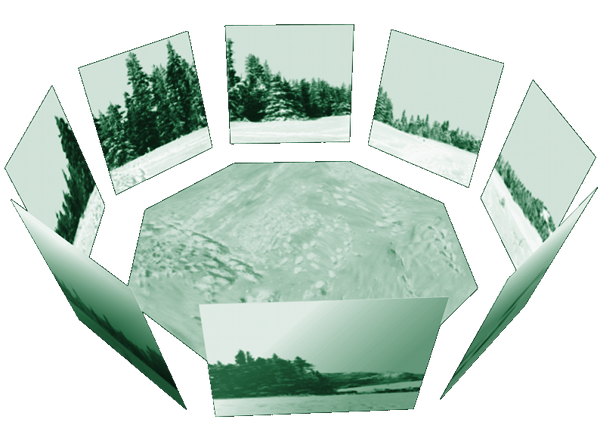
\includegraphics[scale=0.7]{faq_landscape}
%\caption{Figure caption}
\end{figure}

On the negative side, it is more difficult to create this type of
landscape - merging the ground texture with the side textures can prove
tricky. The contents of the \texttt{landscape.ini} file for this
landscape type is also somewhat more complicated than for other
landscape types. Here is the \texttt{landscape.ini} file which describes
the Guereins landscape:

\begin{config}
\texttt{{[}landscape{]}}\\
\texttt{name~=~Guereins}\\
\texttt{type~=~old\_style}\\
\texttt{author~=~Fabien~Chéreau}\\
\texttt{description~=~Guéreins~is~a~small~french~village...}\\
\texttt{nbsidetex~=~8}\\
\texttt{tex0~=~guereins4.png}\\
\texttt{tex1~=~guereins5.png}\\
\texttt{tex2~=~guereins6.png}\\
\texttt{tex3~=~guereins7.png}\\
\texttt{tex4~=~guereins8.png}\\
\texttt{light4~=~guereins8-lgt.png}\\
\texttt{tex5~=~guereins1.png}\\
\texttt{tex6~=~guereins2.png}\\
\texttt{tex7~=~guereins3.png}\\
\texttt{nbside~=~8}\\
\texttt{side0~=~tex0:0:0.005:1:1}\\
\texttt{side1~=~tex1:0:0.005:1:1}\\
\texttt{side2~=~tex2:0:0.005:1:1}\\
\texttt{side3~=~tex3:0:0.005:1:1}\\
\texttt{side4~=~tex4:0:0.005:1:1}\\
\texttt{side5~=~tex5:0:0.005:1:1}\\
\texttt{side6~=~tex6:0:0.005:1:1}\\
\texttt{side7~=~tex7:0:0.005:1:1}\\
\texttt{groundtex~=~guereinsb.png}\\
\texttt{fogtex~=~fog.png}\\
\texttt{nb\_decor\_repeat~=~1}\\
\texttt{decor\_alt\_angle~=~40}\\
\texttt{decor\_angle\_shift~=~-22}\\
\texttt{decor\_angle\_rotatez~=~0}\\
\texttt{ground\_angle\_shift~=~-22}\\
\texttt{ground\_angle\_rotatez~=~45}\\
\texttt{fog\_alt\_angle~=~20}\\
\texttt{fog\_angle\_shift~=~-3}\\
\texttt{draw\_ground\_first~=~1}
\end{config}

Where:

\begin{itemize}
\item
  \textbf{name} is the name that will appear in the landscape tab of the
  configuration window for this landscape
\item
  \textbf{type} should be ``old\_style'' for the multiple image method.
\item
  \textbf{author} lists the author(s) responsible for images and
  composition.
\item
  \textbf{description} gives a short description visible in the
  selection panel. The text will be superseded by optional
  description..utf8 files.
\item
  \textbf{nbsidetex} is the number of side textures for the landscape.
\item
  \textbf{tex0 ... tex} are the side texture file names. These should
  exist in the \texttt{.../textures/landscapes} directory in PNG format.
\item
  \textbf{light0 ... light} are optional textures. If they exist, they
  are used as overlays on top of the respective
  tex\textless{}...\textgreater{} files and represent nocturnal
  illumination, e.g. street lamps, lit windows, red dots on towers, sky
  glow by city light pollution, ... Empty panels don't have to exist. If
  you need your light pollution higher in the sky, you must use a
  spherical or fisheye landscape. (New feature, V0.13.1)
\item
  \textbf{nbside} is the number of side textures
\item
  \textbf{side0 ... side} are the descriptions of how the side textures
  should be arranged in the program. Each description contains five
  fields separated by colon characters (:). The first field is the ID of
  the texture (e.g. tex0), the remaining fields are the texture
  coordinates (x0:y0:x1:y1) used to place the texture in the scene. If
  you want to use all of the image, this will just be \texttt{0:0:1:1}.
\item
  \textbf{groundtex} is the name of the ground texture file. (This could
  also be a diagram e.g. indicating the mountain peaks!)
\item
  \textbf{ground} {[}NO LONGER USED{]} used to be the description of the
  projection of the ground texture in the scene.
\item
  \textbf{fogtex} is the name of the texture file for fog in this
  landscape. Note that for this landscape, accurate overlay of fog and
  landscape is only done if \texttt{calibrated=true} and
  \texttt{tan\_mode=true}.
\item
  \textbf{fog} {[}NO LONGER USED{]} used to be the description of the
  projection of the fog texture in the scene.
\item
  \textbf{nb\_decor\_repeat} is the number of times to repeat the side
  textures in the 360 panorama. (Photo panoramas should have ``1'' here)
\item
  \textbf{decor\_alt\_angle} (degrees) is the vertical angular size of
  the textures (i.e. how high they go into the sky).
\item
  \textbf{decor\_angle\_shift} (degrees) vertical angular offset of the
  scenery textures, at which height are the side textures placed.
\item
  \textbf{decor\_angle\_rotatez} (degrees) angular rotation of the
  scenery around the vertical axis. This is handy for rotating the
  landscape so North is in the correct direction.
\item
  \textbf{ground\_angle\_shift} (degrees) vertical angular offset of the
  ground texture, at which height the ground texture is placed.
\item
  \textbf{ground\_angle\_rotatez} (degrees) angular rotation of the
  ground texture around the vertical axis. When the sides are rotated,
  the ground texture may need to be rotated as well to match up with the
  sides.
\item
  \textbf{fog\_alt\_angle} (degrees) vertical angular size of the fog
  cylinder - how fog looks. Accurate vertical size requires
  \texttt{calibrated=true}.
\item
  \textbf{fog\_angle\_shift} (degrees) vertical angular offset of the
  fog texture - at what height is it drawn. Accurate vertical placement
  requires \texttt{calibrated=true}.
\item
  \textbf{draw\_ground\_first} if 1 the ground is drawn in front of the
  scenery, i.e. the side textures will overlap over the ground texture.
\item
  \textbf{calibrated} (optional, not used in this file). New since
  0.10.6: Only if true, decor\_alt\_angle etc. really work as documented
  above. The (buggy) old code was left to work with the landscapes
  already existing.
\item
  \textbf{tan\_mode} (optional, not used in this file). If true, the
  panorama image must be in in cylindrical, not equirectangular
  projection. Finding \texttt{decor\_alt\_angle} and
  \texttt{decor\_angle\_shift} may be a bit more difficult with this,
  but now (V0.13) works also with calibrated. A fog image created as
  overlay on the pano will be perfectly placed.
\item
  \textbf{decor\_angle\_rotatez} angular rotation of the scenery around
  the vertical axis. This is handy for rotating the landscape so North
  is in the correct direction. If 0, the left edge of \texttt{tex0} is
  due east.
\item
  \textbf{ground\_angle\_shift} vertical angular offset of the ground
  texture, at which height the ground texture is placed. Values above
  -10 are not recommended for non-photographic content due to high
  distortion.
\item
  \textbf{ground\_angle\_rotatez} angular rotation of the ground texture
  around the vertical axis. When the sides are rotated, the ground
  texture may need to be rotated as well to match up with the sides. If
  0, east is up. if North is up in your image, set this to 90.
\item
  \textbf{fog\_alt\_angle} vertical angular size of the fog texture -
  how fog looks.
\item
  \textbf{fog\_angle\_shift} vertical angular offset of the fog texture
  - at what height is it drawn.
\item
  \textbf{draw\_ground\_first} if 1 the ground is drawn before the
  sides, i.e. the side textures may overlap the ground texture if
  \texttt{ground\_angle\_shift\ \&gt;\ decor\_angle\_shift}.
\item
  \textbf{polygonal\_horizon\_list} (optional) is the name of the
  (measured) horizon data file for this landscape. Can be used to query
  horizon transparency (for accurate object rising/setting times)
\item
  \textbf{polygonal\_horizon\_list\_mode} (optional) the two first
  columns in the list are numbers: azimuth and altitude or zenith
  distance, in either degrees or radians or gradians(gon). The value
  must be one of
  azDeg\_altDeg\textbar{}azDeg\_zdDeg\textbar{}azRad\_altRad\textbar{}azRad\_zdRad\textbar{}azGrad\_altGrad\textbar{}azGrad\_zdGrad.
  Default: azDeg\_altDeg
\item
  \textbf{polygonal\_angle\_rotatez} (optional, default=0) Angle
  (degrees) to adjust azimuth. This may be used to apply a (usually)
  small offset rotation, e.g. when you have measured the horizon in a
  grid-based coordinate system like UTM and have to compensate for the
  meridian convergence.
\item
  \textbf{horizon\_line\_color} (optional, default: invisible) used to
  draw a polygonal horizon line.
\item
  \textbf{minimal\_brightness} (optional, default=-1, i.e. use preset
  landscape/minimal\_brightness from global config.ini) Some minimum
  brightness to keep landscape visible.
\item
  \textbf{minimal\_altitude} (optional, default=-2) Some sky elements,
  e.g. stars, are not drawn below this altitude. Under certain
  circumstances you may want to specify something else here. (since
  V0.14)
\end{itemize}

\subsection{landscape.ini {[}location{]} section}\label{landscape.ini-location-section}

An example location section:

\begin{config}
\texttt{{[}location{]}}\\
\texttt{planet~=~Earth}\\
\texttt{latitude~=~+48d10'9.707"}\\
\texttt{longitude~=~+11d36'32.508"}\\
\texttt{altitude~=~83}\\
\texttt{light\_pollution=3}\\
\texttt{atmospheric\_extinction\_coefficient=0.2}\\
\texttt{atmospheric\_temperature=10}\\
\texttt{atmospheric\_pressure=-1}
\end{config}

Where:

\begin{description}
\item[planet] Is the English name of the solar system body for the
  landscape.
\item[latitude] Is the latitude of site of the landscape in degrees,
  minutes and seconds. Positive values represent North of the equator,
  negative values South of the equator.
\item[longitude] Is the longitude of site of the landscape. Positive
  values represent East of the Greenwich Meridian on Earth (or
  equivalent on other bodies), Negative values represent Western
  longitude.
\item[altitude] Is the altitude of the site of the landscape in
  meters.
\item[country] (optional) Name of the country the location is in
\item[state] (optional) Name of the state the location is in
\item[name] (optional) Name of the location
\end{description}

Since 0.11, there are a few more optional parameters that can be loaded
if the according switch is active in the landscape selection panel. If
they are missing, the parameters do not change to defaults.

\begin{description}
\item[light\_pollution] (optional) Light pollution of the site,
  given on the Bortle Scale (1: none ... 9: metropolitan). If negative
  or absent, no change will be made.
\item[atmospheric\_extinction\_coefficient] (optional, no change if
  absent.) Extinction coefficient (mag/airmass) for this site.
\item[atmospheric\_temperature] (optional, no change if absent.)
  Surface air temperature (Degrees Celsius). Used for refraction. . Set
  to -1000 to explicitly declare ``no change''.
\item[atmospheric\_pressure] (optional, no change if absent.)
  Surface air pressure (mbar; would be 1013 for ``normal'' sea-level
  conditions). Used for refraction. Set to -2 to declare ``no change'',
  or -1 to compute from altitude.
\item[display\_fog] (optional, -1/0/1, default=-1) You may want to
  preconfigure setting \textbf{0} for a landscape on the Moon. Set -1 to
  declare ``no change''.
\end{description}

\section{Making a Multi panel Panorama}\label{making-a-multi-panel-panorama}

\begin{figure}[h]
\centering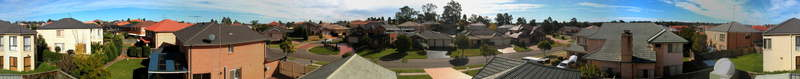
\includegraphics[scale=2.2]{landscape_beaumonthills.jpg}
%\caption{Figure caption}
\end{figure}

This is the only way to get a high resolution panorama and although this
procedure is based on the Microsoft Windows System the basics will apply
to any platform that can run the programs mentioned or similar programs
on the preferred system. If you want a high resolution this is the only
method to use. The first thing needed for a personalised landscape to
superimpose on the horizon display is a 360$\degree$ panorama with a transparent
background. To make this you will need the following:

\begin{itemize}
\item
  A digital camera on a tripod or stable platform
\item
  A program to convert the pictures into a 360$\degree$ panorama
\item
  A program to remove the background and convert the panorama into about
  8 square pictures in PNG format for insertion into Stellarium as the
  sides and if possible a similar square picture of the base you are
  standing on to form the ground. This last requirement is only really
  possible if this area is relatively featureless as the problem of
  knitting a complex base is well nigh impossible.
\item
  Patience. (Maybe a soundproof room so that the swearing wont be heard
  when you press the wrong key and lose an hours work)
\end{itemize}

\subsection{The Camera}\label{the-camera}

Digital cameras are easy and cheaply available these days so whatever
you have should do. One mega-pixel resolution is quite sufficient.

The camera needs to be mounted on a tripod so that reasonably orientated
pictures can be taken. Select a time of day that is quite bright with a
neutral cloudy sky so there will be no shadows and a sky of the same
overall texture. This will make it easier to remove later. The pictures
were all saved in the JPG format which was used as the common format for
all processes up to the removal of the background.

With a camera that takes 4:3 ratio pictures I found 14 evenly spaced
pictures gave the best 360$\degree$ panorama in the program I used to produce
it.

\subsection{Processing into a
Panorama}\label{processing-into-a-panorama}

This is the most complicated part of the process of generating the
panorama. I used two separate programs to do this. Firstly I used The
Gimp to re size the panels to 1024x768 and so make them easier to handle
in the panorama program.

When I had my 14 processed pictures I inserted them into the panorama
program. I first used a program called the Panorama Factory. Version 1.6
is a freebee that works well and can be downloaded from the internet - a
Google search will find it. I later used version 3.4 that is better and
cost about \$40 off the Internet. This program has many options and can
be configured to suit most cameras and can make a seamless 360$\degree$ panorama
in barrel form that will take a highly trained eye to find where the
joins occur.

The resulting panorama was then loaded into The Gimp and trimmed to a
suitable size. Mine ended up 14024 x 1601 pixels. I trimmed the vertical
size to 1024 by cutting back then stretched the 14024 to 14336 pixels,
with almost no distortion, that would allow cutting into 14 1024 x1024
pictures at a later date. If the height of the panorama had been greater
I could have made fewer pictures and so shown more of the foreground.
See figure {[}fig:panorama360{]}.

If you have prominent foreground items like posts wires etc. that occur
in adjacent pictures the panorama program will have difficulty in
discerning them because of the 3D effect and may give double images. I
overcame this by painting out the offending item by cut and paste
between the two pictures. Quite easy with a little practice using the
zoom in facility and I found the MSpaint program the easiest to do this
in.

\begin{figure}[h]
\centering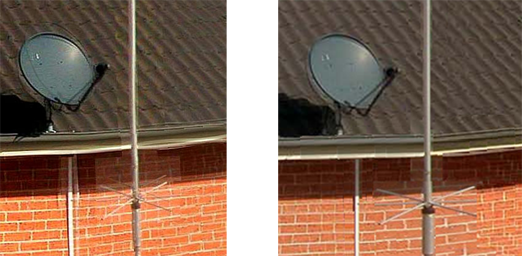
\includegraphics[scale=2.0]{BEAU-3c}
%\caption{Figure caption}
\end{figure}

\subsection{Removing the background to make it
transparent}\label{removing-the-background-to-make-it-transparent}

This is the most complex part of the process and requires a program that
can produce transparency to parts of your picture, commonly called an
alpha channel. Two programs I know of will do this. The very expensive
and sophisticated Adobe Photoshop and a freebee called The Gimp. I used
photoshop to cut the full panorama into 1024 x 1024 textures because it
was the easiest to do accurate cutting but it can be done in TheGimp as
well.

I first used Photoshop to produce the alpha channel because it was the
only way I knew but I now use the GIMP as it is much easier to process
the individual textures than removing the background from the full
panorama.

\begin{enumerate}
\item
  Load the 1st section into TheGimp
\item
  Next create a new empty picture 1024 x 1024 then use the advanced tab
  to make the background color transparency. Copy the original texture
  onto this new picture base so that it exactly fits the frame then
  select layer from the menu and press anchor. This will create a new
  picture with with an alpha channel. By using the select by color and
  lasso etc cut out the parts you don't want this will expose the
  checkerboard background. When you are happy with the removal save the
  texture in *.png format to preserve the alpha layer.
\item
  Do the same with the remaining pictures to make all the components of
  the landscape.
\item
  Make a new directory for the landscape. This should be a sub-directory
  of either the /landscapes or /landscapes directory. The name of the
  directory should be unique to your landscape, and is the landscape ID.
  The convention is to use a single descriptive word in lowercase text,
  for example gueriens. Place your pictures your new directory.
\item
  In your new landscape directory, create a new file called
  landscape.ini file (I used wordpad). Add a line for the
  {[}landscape{]} section. It's probably easiest to copy the
  landscape.ini file for the Gueriens landscape and edit it. Edit the
  name Guereins in every instance to the name you have given your
  landscape. Don't forget to make the number of tex entries agree with
  the number of your pictures. If you haven't made a groundtex picture
  use one of the existing ones from the file or make a square blank
  picture of your own idea. Because I took my pictures from the roof of
  the house I used an edited picture of the roof of my house from Google
  Earth. It was pretty cruddy low resolution but served the purpose.
\item
  Next you need to orientate your picture North with true North. This is
  done roughly by making the arrangement of side1 to siden suit your
  site as close as possible. Now you need to edit the value of
  decor\_angle\_rotatez to move your landscape in azimuth. Edit
  decor\_alt\_angle to move you landscape in altitude to align your
  visible horizon angle. Edit ground\_angle\_rotatez to align your
  ground with the rest of the landscape. Leave the other entries they
  are suitable as is.
\end{enumerate}

After re-starting Stellarium, your landscape will appear in the
landscape folder of the main menu , and can be selected as required.

\section{Making a Spherical Panorama}
\label{making-a-spherical-panorama}

A simpler method of making a panorama is to use the spherical method.
These can be made to create the full panorama using the program
Autostitch. The big advantage of the spherical panorama is that it does
not need a ground panel. However the drawback with the Spherical
panorama is that few computer video cards will reproduce a panorama
larger than 4096 x 2048 pixels and many will not do better than 2048 x
1024 pixels

\begin{figure}[h]
\centering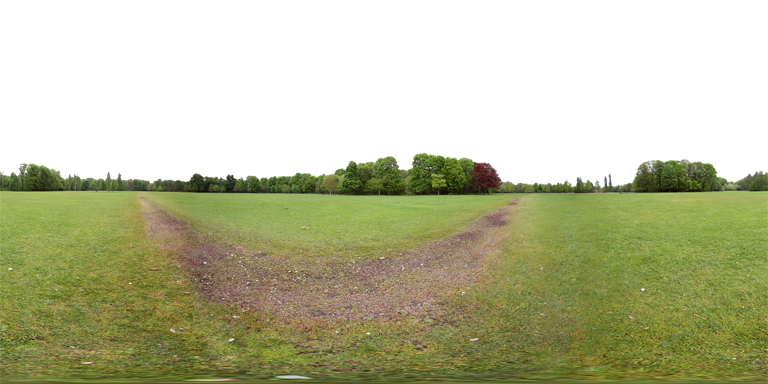
\includegraphics{egarden}
%\caption{Figure caption}
\end{figure}

The Autostitch program is quite easy to use. Make sure your panorama
shots take the ground almost up to your feet and follow the instructions
in the readme file. \href{http://www.example.com}{link title} When the
panorama is finished it will be in *,jpg format. This will need to be
converted to a *.png with transparent background (alpha layer) and have
the sky removed. This can be done in TheGimp as in the multi-panel type.
When the sky is removed make sure you save the landscape in *.png
format.

My computer will only do 2048 by 1024, If I try to load a larger type I
just get a white screen. With this problem I used the following
procedure to make the spherical into a four panel multi-panel landscape
with a very effective ground that matched well

\subsection{Converting a Spherical Panorama into a Multi Panel}
\label{converting-a-spherical-panorama-into-a-multi-panel}

Most computers with standard video cards will not display spherical
panoramas larger than 4096 x 2048 and some will not even go beyond 2048
x 1024. This makes rather poor resolution panaoramas. OK for planets but
not very pretty for your local environment. If the panorama can have a
horizontal section cut out that can keep the detail within a 1024
vertical boundary it is ideal for processing into 1024 x 1024 sections.
When you have the sections proceed as with the previous description

\begin{figure}[h]
\centering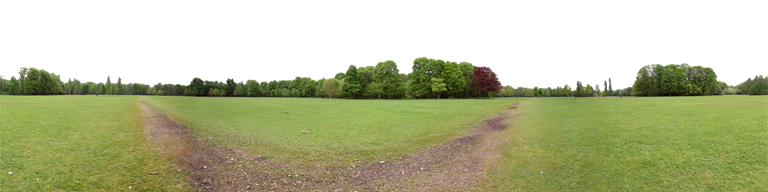
\includegraphics{egarden-narrow}
%\caption{Figure caption}
\end{figure}

I made the egarden into a 4096 x 1024 quite easily because there was a
lot of blank space above the horizon. This would allow 4 panels 1024 x
1024 pixels.in fact if I had a 8192 x 4096 panorama I could have made it
into 8 1024 x 1024 panels. This would have given me quite a high
resolution horizon

\begin{figure}[h]
\centering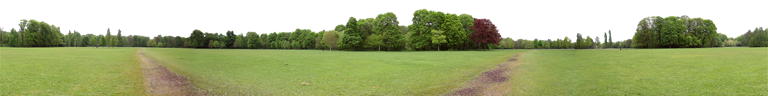
\includegraphics{egarden-narrow-2}
%\caption{Figure caption}
\end{figure}


\begin{enumerate}
\item
  Load the sections into TheGimp and process them into 1024 x 1024
  textures with alpha layers as before.
\item
  Next use a 2048 x 1024 version of the panorama in Stellarium. Drag the
  screen around so it produces a centralised picture on the Stellarium
  screen of the ground at the highest resolution possible and take a
  screen shot. This screen shot can be then processed into a quite
  effective ground texture in TheGimp that can be adjusted to match the
  rest of the panorama.
  \begin{figure}[h]
  \centering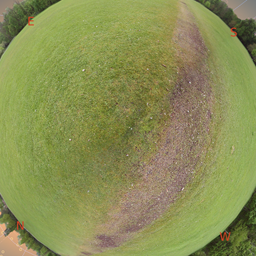
\includegraphics[scale=2.0]{egardembase}
  %\caption{Figure caption}
  \end{figure}
\item
  Make a new directory etc. for the landscape.
\item
  You can make it fit using the variablein the landscape.ini file
  decor\_alt\_angle=xx decor\_angle\_shift=xx and
  decor\_angle\_rotatez=xx.Then the ground can be matched with
  ground\_angle\_shift=xx and ground\_angle\_rotatez=xx.
\item
  Make sure the draw\_ground\_first=1 to ensure that the main panorama
  overplays the ground
\end{enumerate}

After re-starting Stellarium, your landscape will appear in the
landscape tab of the main menu, and can be selected as required.

When the panorama is finished it will be in *.jpg format. It will need
to be converted to a *.png with transparent background (alpha layer) and
have the sky removed. This is done in TheGimp as in the multipanel type.
When the sky is removed make sure you save the landscape in *.png
format.

The drawback with the spherical panorama is that few computer video
cards will reproduce a panorama larger than 4096 x 2048 pixels in
Stellarium and many will not do better than 2048 x 1024 pixels.

My computer will only do 2048 by 1024, If I try to load a larger type I
just get a white screen. With this problem I used the following
procedure to make the spherical into a four panel multi panel landscape
with a very effective ground that matched well.

\section{Making a Fish eye Panorama}
\label{making-a-fish-eye-panorama}

This sort of panorama needs a very expensive fisheye lens on your
camera. It is really only practical for a planetarium display to give a
simple more or less silouette landscape where the ground is completely
obscured. It can only be used with quite small pictures of no more than
1024 x 1024 pixels. Once you have your fisheye texture it must still be
processed in TheGimp to remove the sky and convert into an alpha layer
texture

\begin{figure}[h]
\centering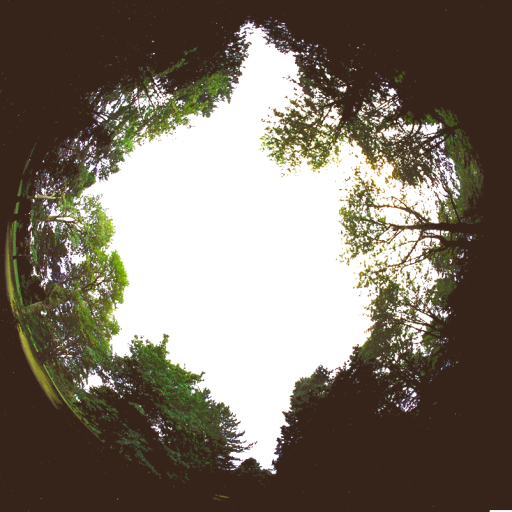
\includegraphics[scale=3.0]{trees_512}
%\caption{Figure caption}
\end{figure}

The sample supplied with Stellarium is called trees. The horizon needs
to be identified and the picture sized so that the panorama above the
horizon is sited to be about 80\% of the total extent and the the
balance of the border filled with a dark colour right up to the horizon.
This will make the horizon in your landscape at 0 degrees.

It is possible to make a synthetic fisheye texture using the same method
as making a ground from a spherical panorama but it is hardly worth the
trouble as even a simple 2048 x 1024 pixel sperical will give a far
better result.

%%% Local Variables: 
%%% mode: latex
%%% TeX-master: "guide"
%%% End: 

%% Stellarium User Guide

\chapter{Deep-Sky Objects}%\label{deep-sky-objects}
\label{ch:dso}

Extended objects are those which are external to the solar system, and
are not point-sources like stars. These are generally known as
\indexterm{deep-sky objects} or DSO. Extended objects include
galaxies, planetary nebulae and star clusters. These objects may or
may not have images associated with them. Stellarium also comes with a
catalogue with over 14,000 extended objects containing the combined
data from many catalogues, with 190 images.

Since version 0.10.0 Stellarium uses new method of displaying
textures using the ``json'' cataloguing system. At the same time the
Simbad online catalogue was added to the search feature, making the catalog
somewhat redundant and used now only as a first search point or if there
is no internet connection.

If the object has a name (not just a catalogue number), you should add
one or more records to the \file{.../nebulae/default/names.dat} file
(where \file{...} is either the installation directory or the user
directory). See section~\ref{dso:modifyingNamesDat}
\emph{\protect\hyperlink{Modifyingux5fnames.dat}{Modifying names.dat}}
for details of the file format.

If you wish to associate a texture (image) with the object, you must now
add a record to the \file{.../nebulae/default/textures.json} file. See
section~\ref{dso:modTexturesJson} for details of the file format.

Nebula images should have dimensions which are integer powers of two,
i.e. 1, 2, 4, 8, 16, 32, 64, 128, 256, 512, 1024 ... pixels along each
side. If this requirement is not met, your textures may not be visible,
or graphics performance may be seriously impacted. PNG or JPG formats
are both supported.

\section{GUI for managing Deep-Sky Objects}%\label{gui-for-manage-by-deep-sky-objects}
\label{sec:dso:gui}

\begin{figure}[h]
\centering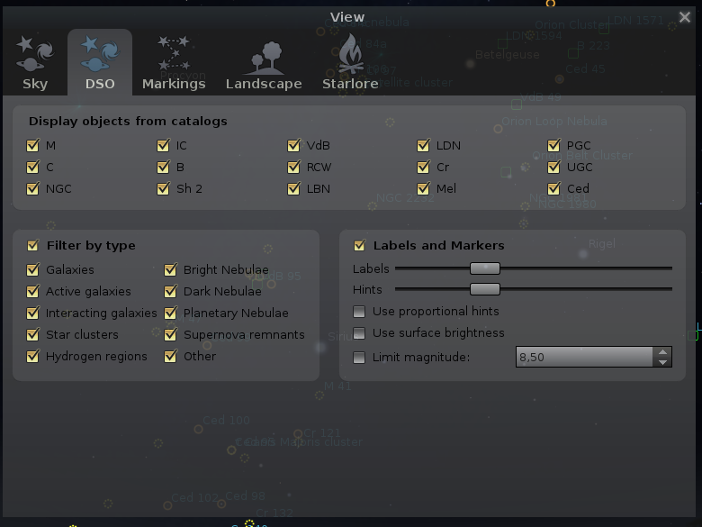
\includegraphics{DSO_GUI}
%\caption{Figure caption}
\end{figure}

\section{Stellarium DSO Catalog}%\label{stellarium-dso-catalog}
\label{sec:dso:catalog}

Stellarium's DSO Catalog contains over 1400 objects and is available
for end users as collection of files:

\begin{itemize}
\item
  \texttt{catalog.txt} - Stellarium DSO Catalog in ASCII format for
  editing data;
\item
  \texttt{catalog.dat} - Stellarium DSO Catalog in binary format for
  usage within Stellarium;
\item
  \texttt{names.dat} - list of proper names of the objects from
  \texttt{catalog.dat} file.
\end{itemize}

ASCII file can be converted into binary format through enabling option
\texttt{devel/convert\_dso\_catalog\ =\ true} in the \texttt{config.ini}
file. The file \texttt{catalog.txt} should be put to the directory
\texttt{.../nebulae/default/}.

Stellarium DSO Catalog contains data and supports the designations for
follow catalogues:

\begin{description}
\item[NGC]  New General Catalogue 
\item[IC] Index Catalogue 
\item[M] Messier Catalog
\item[C] Caldwell Catalogue 
\item[B] Barnard Catalogue 
\item[Sh2] Sharpless Catalogue 
\item[VdB] Van den Bergh Catalogue of reflection nebulae 
\item[RCW]  A catalogue of H$\alpha$-emission regions in the southern Milky Way 
\item[LDN]  Lynds' Catalogue of Dark Nebulae 
\item[LBN]  Lynds' Catalogue of Bright Nebulae 
\item[Cr] Collinder Catalogue 
\item[Mel]  Melotte Catalogue of Deep Sky Objects 
\item[PGC]  HYPERLEDA. I. Catalog of galaxies \footnote{Partial support}
\item[UGC]  The Uppsala General Catalogue of Galaxies \footnote{Partial    support}
\item[Ced]  Cederblad Catalog of bright diffuse Galactic nebulae 
\end{description}


\subsection{Modifying catalog.dat}\label{modifying-catalog.dat}

This section is described inner structure of files \texttt{catalog.dat}
(has binary format) and \texttt{catalog.txt} (has ASCII format).
Stellarium can convert ASCII file into the binary format file for usage
within planetarium.

Each line contains one record, each record consisting of the following
fields with \emph{tab} char as delimiter:

\begin{longtabu} to \textwidth {l|l|X}
\toprule
\emph{Column} & \emph{Type} & \emph{Description}\tabularnewline
\midrule
1 & integer & Deep-Sky Object Identificator\tabularnewline
2 & float & RA (decimal degrees)\tabularnewline
3 & float & Dec (decimal degrees)\tabularnewline
4 & float & B magnitude\tabularnewline
5 & float & V magnitude\tabularnewline
6 & string & Object type (Possible values see in table
\emph{\protect\hyperlink{Typesux5fofux5fObjects}{Types of
Objects}}).\tabularnewline
7 & string & Morphological type of object\tabularnewline
8 & float & Major axis size or radius (arcmin)\tabularnewline
9 & float & Minor axis size (arcmin)\tabularnewline
10 & integer & Orientation angle (degrees)\tabularnewline
11 & float & Redshift\tabularnewline
12 & float & Error of redshift\tabularnewline
13 & float & Parallax (mas)\tabularnewline
14 & float & Error of parallax (mas)\tabularnewline
15 & float & Non-redshift distance (Mpc for galaxies, kpc for other
objects)\tabularnewline
16 & float & Error of non-redsift distance (Mpc for galaxies, kpc for
other objects)\tabularnewline
17 & integer & NGC number (New General Catalogue)\tabularnewline
18 & integer & IC number (Index Catalogue)\tabularnewline
19 & integer & M number (Messier Catalog)\tabularnewline
20 & integer & C number (Caldwell Catalogue)\tabularnewline
21 & integer & B number (Barnard Catalogue)\tabularnewline
22 & integer & Sh2 number (Sharpless Catalogue)\tabularnewline
23 & integer & VdB number (Van den Bergh Catalogue of reflection
nebulae)\tabularnewline
24 & integer & RCW number (A catalogue of H$\alpha$-emission regions in the
southern Milky Way)\tabularnewline
25 & integer & LDN number (Lynds' Catalogue of Dark
Nebulae)\tabularnewline
26 & integer & LBN number (Lynds' Catalogue of Bright
Nebulae)\tabularnewline
27 & integer & Cr number (Collinder Catalogue)\tabularnewline
28 & integer & Mel number (Melotte Catalogue of Deep Sky
Objects)\tabularnewline
29 & integer & PGC number (HYPERLEDA. I. Catalog of galaxies);
partial\tabularnewline
30 & integer & UGC number (The Uppsala General Catalogue of Galaxies);
partial\tabularnewline
31 & string & Ced number (Cederblad Catalog of bright diffuse Galactic
nebulae)\tabularnewline
\bottomrule
\end{longtabu}

\subsubsection{Types of Objects}\label{types-of-objects}

Possible values for type of objects in the file \texttt{catalog.dat}.

\begin{longtabu} to \textwidth {l|X}
\toprule
\emph{Type} & \emph{Description}\tabularnewline
\midrule
G & Galaxy\tabularnewline
GX & Galaxy\tabularnewline
AGX & Active Galaxy\tabularnewline
RG & Radio Galaxy\tabularnewline
IG & Interacting Galaxy\tabularnewline
GC & Globular Cluster\tabularnewline
OC & Open Cluster\tabularnewline
NB & Nebula\tabularnewline
PN & Planetary Nebula\tabularnewline
DN & Dark Nebula\tabularnewline
RN & Reflection Nebula\tabularnewline
C+N & Cluster associated with nebulosity\tabularnewline
HII & HII Region\tabularnewline
SNR & Supernova Remnant\tabularnewline
BN & Bipolar Nebula\tabularnewline
EN & Emission Nebula\tabularnewline
SA & Stellar Association\tabularnewline
SC & Star Cloud\tabularnewline
CL & Cluster\tabularnewline
IR & Infra-Red Object\tabularnewline
QSO & Quasar\tabularnewline
Q? & Possible Quasar\tabularnewline
ISM & Interstellar Matter\tabularnewline
EMO & Emission Object\tabularnewline
LIN & LINEAR-type Active Galaxies\tabularnewline
BLL & BL Lac Object\tabularnewline
BLA & Blazar\tabularnewline
MOC & Molecular Cloud\tabularnewline
YSO & Young Stellar Object\tabularnewline
PN? & Possible Planetary Nebula\tabularnewline
PPN & Protoplanetary Nebula\tabularnewline
$\ast$ & Star\tabularnewline
$\ast\ast$ & Double Star\tabularnewline
MUL & Multiple Star\tabularnewline
\emph{empty} & Unknown type, catalog errors, \emph{Unidentified Southern
Objects} etc.\tabularnewline
\bottomrule
\end{longtabu}

\subsection{Modifying names.dat}%\label{modifying-names.dat}
\label{sec:dso:modifyingNamesDat}

Each line in the \file{names.dat} file contains one record. A record
relates an extended object catalogue number (from \file{catalog.dat})
with a name. A single catalogue number may have more than one record in
this file.

The record structure is as follows:

\begin{longtabu} to \textwidth {l|l|l|X}
\toprule
\emph{Offset} & \emph{Length} & \emph{Type} & \emph{Description}\tabularnewline
\midrule
0 & 5 & \%5s & Designator for catalogue (prefix)\tabularnewline
5 & 15 & \%d & Identificator for object in the catalog\tabularnewline
20 & 60 & \%s & Proper name of the object (translatable)\tabularnewline
\bottomrule
\end{longtabu}

If an object has more than one record in the \texttt{names.dat} file,
the last record in the file will be used for the nebula label.

\subsection{Modifying textures.json}%\label{modifying-textures.json}
\label{sec:dso:modifyingTexturesJson}

This file is used to describe each nebula image. The file structure
follows the JSON format, a detailed description of which may be found at
. The textures.json file which ships with Stellarium has the following
structure:

\begin{itemize}
\item
  serverCredits (optional) - a structure containing the following
  key/value pairs:

  \begin{itemize}
  \item
    short - a short identifier of a server where the json file is found,
    e.g. ``ESO''
  \item
    full - a longer description of a server, e.g. ``ESO Online Digitised
    Sky Survey Server''
  \item
    infoURL - a URL pointing at a page with information about the server
  \end{itemize}
\item
  imageCredits - a structure containing the same parts as a
  serverCredits structure but referring to the image data itself
\item
  shortName - an identifier for the set of images, to be used inside
  Stellarium
\item
  minResolution - minimum resolution, applies to all images in the set,
  unless otherwise specified at the image level
\item
  maxBrightness - the maximum brightness of an image, applies to all
  images in the set, unless otherwise specified at the image level
\item
  subTiles - a list of structures describing indiviual image tiles, or
  referring to another json file. Each subTile may contain:

  \begin{itemize}
  \item
    minResolution
  \item
    maxBrightness
  \item
    worldCoords
  \item
    subTiles
  \item
    imageCredits
  \item
    imageUrl
  \item
    textureCoords
  \end{itemize}
\item
  shortName (name for the whole set of images, e.g. ``Nebulae'')
\item
  miniResolution (applies to all images in set)
\item
  alphaBlend (applies to all images in set)
\item
  subTiles list of images. Each image record has the following
  properties:

  \begin{itemize}
  \item
    imageCredits (itself a list of key/pairs)
  \item
    imageUrl (e.g. file name)
  \item
    worldCoords (a list of four pairs of coordinates representing the
    corners of the image)
  \item
    textureCoords (a list of four pairs of corner descriptions. i.e.
    which is top left of image etc)
  \item
    minResolution (over-rides file-level setting)
  \item
    maxBrightness
  \end{itemize}
\end{itemize}

Items enclosed in Quotation marks are strings for use in the program.
Syntax is extremely important. Look at the file with a text editor to
see the format. Items in \textless{}\textgreater{} are user provided
strings and values to suit the texture and source.

\texttt{Line~1~“imageCredits”:~\{“short”~:~“}\texttt{”~:~“infoUrl”:~}\href{http://}{\texttt{http://}}\texttt{\},~}\\
\texttt{Line~2~“imageUrl”~:~“}\texttt{”,~}\\
\texttt{Line~3~“worldCoords”~:~\textless{}~decimal~numerical~values~of~the~J2000~coordinates~of~the~corners~of~the~texture~\textgreater{}~These~values~displayed~to~4~decimal~places~in~the~format~of~the~texture~coordinates~}\\
\texttt{Line~4~“textureCoords”~:~{[}{[}{[}~0,0{]},{[}1,0{]},{[}1,1{]},{[}0,1{]}{]}{]},~Where~0,0~is~South~Left~,~1,0~the~South~Right~,~1,1~North~Right~,~0,1~North~Left~corners~of~texture~Format~=~RA~in~degrees,~Dec~in~degrees~}\\
\texttt{Line~5~“MinResolution”~:~}\texttt{,~}\\
\texttt{Line~6~“maxBrightness”~:~\textless{}~a~numerical~vale~representing~the~absolute~brightness~for~the~display\textgreater{}~}

Calculating of the coords of the corners of the images (plate solving)is
a time consuming project and needs to be fine tuned from the screen
display. As most images will be two dimensional, display on a spherical
display will limit the size to about 1 degree before distortion becomes
evident. Larger displays can be sectioned into a mosaic of smaller
textures for a more accurate display

\section{Adding Extra Nebulae Images}%\label{adding-extra-nebulae-images}
\label{sec:dso:adding_images}

\subsection{\texorpdfstring{Preparing a photo for inclusion to the \file{textures.json} file}{Preparing a photo for inclusion to the textures.json file}}
\label{sec:dso:preparing-a-photo}

\begin{figure}[h]
\centering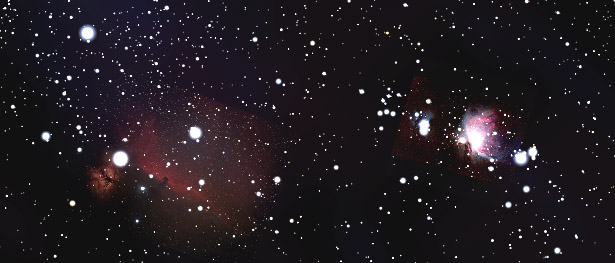
\includegraphics{nebula-display}
\caption{Screen shot of nebula images displayed in Stellarium}
\end{figure}

The first step is to take a photo of the object you wish to display in
Stellarium as a screen backdrop. Then when you have the picture you will
need align it so that north is directly up and not inverted side to side
or up and down as can happen with photos taken with a diagonal mirror in
the path. Next you will need to crop the picture, setting the main
feature at the centre and making the cropped size a factor of $2^n$ eg. 64,
128, 256, 512 or 1024 pixels square. When cropping make sure you leave
at least five prominent background stars.

The next step is to process your photo to make the background
black,black. This will ensure that your background will meld with the
Stellarium background and not be noticed. Suitable programs to do all
this are The Gimp (free in keeping with the Stellarium spirit) or
Photoshop if you can afford it.

When you have your prepared image you will need to plate solve it using
at least 6 known GSC stars that can be identified. That is why the
cropping with plenty of stars was necessary. When the plate is solved
you will need to find the J2000 coordinates of the corners and convert
them to decimal values to form the world coordinates in the
\file{textures.json} file.

\begin{figure}[h]
\centering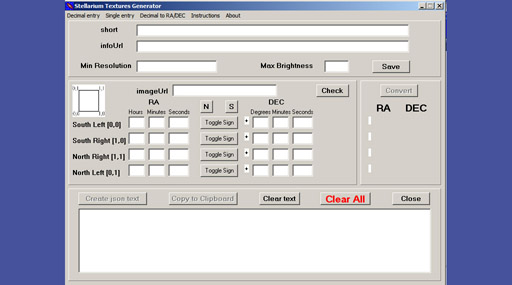
\includegraphics{EQ-Decimal.jpg}
\caption{A program to convert Equatorial coordinates into decimal
form and write a \texttt{textures.json} insert}
\end{figure}

The program in the picture can accept the corner coordinates of a
texture in your plate solving program into decimal values and write an
insert for the \texttt{textures.json} file. It is available as a freebee
from
\url{http://www.madpc.co.uk/~peterv/astroplover/equipnbits/Stellariumtextures.zip}

\begin{figure}[h]
\centering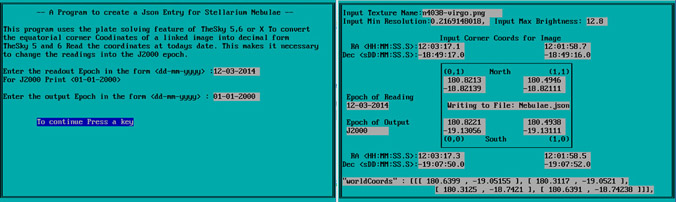
\includegraphics{pix-4.jpg}
\end{figure}

Here is a second program written in Qb64(gl)that will perform the same
task but allows manipulation of the epochs.
\url{http://barry.sarcasmogerdes.com/stellarium/uploads/writejsoninsert.zip}

\subsection{Plate Solving}\label{plate-solving}

Suitable programs that can accept your picture and calculate its corner
coordinates are hard to find. I have only found one that suits our
purpose and it is another expensive planetarium program, TheSkyX Pro.
However the older versions TheSky5 and 6 Pro will also do the job if
suitably configured although I could not solve the test program with the
TheSky6 that uses the same procedure as TheSky5 .

These programs have a link feature that can match your photo to the
selected area of the screen and superimpose it on the display with a box
around your photo provided it can match at least 6 stars from the GSC
that is included with the program. When this is fitted you can read the
corner coordinates of your texture in the Status bar by selecting them
with a mouse. TheSkyX can read these coordinates in J2000 values and
uses textures in the fits format but the earlier programs only read the
coordinates of the current program date. To read the J2000 coordinates
it is necessary to re start the program with the date set to 1-1-2000

To add the picture to TheSky5 you need first make a mono 8 bit version
of the photo and place it on the clipboard. Run TheSky and centre on the
object centre. Look in the Tools menu for the image link and select
setup. Tick show image frame to put a frame around the image.

Paste the clipboard image on the display and use the zoom and position
controls to get it as close to the size and position as possible by
visually matching stars. Go to the menu again and click on link wizard.
If you have been successful the window will show the number of stars
matched and the option to accept or continue. Accept and you will now
see all the matched stars have overlaid the picture. You can now read
off the corner coordinates from the status bar starting at the bottom
(south) left and continuing counter clockwise to the top (north) left.

\subsection{\texorpdfstring{Processing into a \texttt{textures.json}
insert}{Processing into a textures.json insert}}\label{processing-into-a-textures.json-insert}

Place your image in the \texttt{*.png} format in the
\texttt{.../nebulae/default/} folder. Ensure that the name matches the
\texttt{textures.json} entry.

Once you have the corner coordinates of your photo you can add them to
the decimal converter program and it will write an insert
\texttt{nebula.json} as a text file that you can paste directly into the
\texttt{textures.json} file that is in the \texttt{.../nebulae/default/}
folder.

Save the \texttt{textures.json} file with the new insert and run
Stellarium. Select the object in the Object selection window and slew to
it. Your image should be there and with a bit of luck it will nicely
overlay the stars in the Stellarium program. However this only rarely
happens so a little bit of tweaking of the json worldcoords will be
needed to get a perfect match. Select the telescope (equatorial mode).
This will show the area with north up. Select each corner in sequence
and make small changes to the coordinates. Re start Stellarium each time
and check if you have moved the right direction. Continue with each
corner until all the stars match. With a little bit of practice this
will be done in about 10 minutes.


%%% Local Variables: 
%%% mode: latex
%%% TeX-master: "guide"
%%% End: 
 %% Maybe DSO is more a reference chapter? --> Appendix in this case? Or split?


%----------------------------------------------------------------------------------------
%	PART III
%----------------------------------------------------------------------------------------

\part{Extending Stellarium}
\chapterimage{chapter-t3-bg} % Chapter heading image

\chapter{Plugins}
\label{ch:Plugins}

Starting with version 0.10.3, Stellarium's packages have included a steadily growing number of
plug-ins: Angle Measure, Compass Marks, Oculars, Telescope Control, Text
User Interface, Satellites, Solar System Editor, Time Zone, Historical
Supernovae, Quasars, Pulsars, Exoplanets, Observability analysis, ArchaeoLines, Scenery3D. All
these plug-ins are ``built-in'' in the standard Stellarium distribution
and DON'T need to be downloaded separately.

%% TODO: Are there still downloadable plugins?

\section{Enabling plugins}
\label{sec:Plugins:EnablingPlugins}

%\begin{figure}[h]
%\centering\includegraphics{sat_howto_01.jpg}
%\end{figure}

To enable a plugin:

\begin{enumerate}
\item Open the \textbf{Configuration dialog} (press \key{F2} or use
  the left tool bar button \guibutton[0.35]{0.1}{btd_config})
\item Select the \textbf{Plugins} tab
\item Select the plugin you want to enable from the list
\item Check the \textbf{Load at startup} option
\item Restart Stellarium
\end{enumerate}

\noindent If the plugin has configuration options, the
\textbf{configuration} button will be enabled when the plugin has been
loaded and clicking it will open the plugin's configuration
dialog. When you only just activated loading of a plugin, you must
restart Stellarium to access the plugin's configuration dialog.

\section{Data for plugins}
\label{sec:Plugins:DataForPlugins}

Some plugins contain files with different data, e.g., catalogs. JSON is a
typical format for those files and you can edit its content manually. Of
course, each plugin has a specific format of data for the own catalogs, and
you should read documentation for the plugin before editing of its catalog.

You can read some common instructions for editing catalogs of plugins
below. In this example we use file name \file{catalog.json} for
identification of catalog for a typical plugin.

You can modify the \file{catalog.json} files manually using a text
editor. \textbf{If you are using Windows, it is strongly recommended to
use an advanced text editor such as
Notepad++\footnote{\url{http://notepad-plus-plus.org/}}} to avoid problems with
end-of-line characters. (It will also color the JSON code and make it
easier to read.)

\textbf{Warning}: Before editing your \file{catalog.json} file, make a
backup copy. Leaving out the smallest detail (such as a comma or
forgetting to close a curly bracket) will prevent Stellarium from
starting.

As stated in section~\ref{Ch:FilesAndDirectories}, the path to the
directory\footnote{This is a hidden folder, so in order to find it you
  may need to change your computer's settings to display hidden files
  and folders.} which contains \file{catalog.json} file is something
like:

\begin{description}
\item[Windows]
  C:\textbackslash Users\textbackslash\textbf{UserName}\textbackslash AppData\textbackslash Roaming\textbackslash Stellarium\textbackslash modules\textbackslash \textit{PluginName}
\item[Mac OS X]
  \textbf{HomeDirectory}/Library/Preferences/Stellarium/modules/\textit{PluginName}
\item[Linux and UNIX-like OS]
  \textasciitilde{}/.stellarium/modules/\textit{PluginName}
\end{description}



%%% Local Variables: 
%%% mode: latex
%%% TeX-master: "guide"
%%% End: 

\chapterimage{chapter-bg.png} % Chapter heading image
%% Part of Stellarium User Guide
%% Status: 2015-12-30 Some parts collected from wiki.
%%         2016-04-05 GZ changed to have 1 chapter per plugin for a better structure. This file may be split up later. 
%% TODO: All plugins! And give a better structure than just by alphabet.

\chapter{Built-in Plugins}
Since version 0.10.3, Stellarium's packages include a number of plug-ins.

\section{Angle Measure Plugin}
\label{sec:plugins:AngleMeasure}

%\url{http://porpoisehead.net/images/plugin-angle-measure.jpg}

The Angle Measure plugin is a small tool which is used to measure the
angular distance between two points on the sky. 

\begin{quotation}\small
\noindent\emph{goes misty eyed}\\ 
I recall measuring the size of the Cassini Division when I was a student.
It was not the high academic glamor one might expect\ldots It was cloudy\ldots
It was rainy\ldots The observatory lab had some old scopes set up at one
end, pointing at a \emph{photograph} of Saturn at the other end of the
lab. We measured. We calculated. We wished we were in Hawaii. A picture
is worth a thousand words.
\end{quotation}

\subsection{Using the plugin}
\label{sec:plugins:AngleMeasure:using}

\begin{enumerate}
\item
  Enable the tool by clicking the tool-bar button, or by pressing
  \key{Control-A}. A message will appear at the bottom of the screen
  to tell you that the tool is active.
\item
  Drag a line from the first point to the second point using the left
  mouse button
\item
  To clear the measurement, click the right mouse button
\item
  To deactivate the angle measure tool, press the tool-bar button again,
  or press \key{Control-A} on the keyboard.
\end{enumerate}

\newpage

\section{Bright Novae Plugin}
\label{sec:plugins:BrightNovae}

The Bright Novae plugin provides visualization of some bright novae in
the Milky Way galaxy (Fig.~\ref{fig:NovaCygni1975}).

%Example (\href{http://en.wikipedia.org/wiki/V1500_Cygni}{\textbf{Nova
%Cygni 1975}}, also known as \textbf{V1500 Cyg}):

\begin{figure}[h]
\includegraphics[width=\textwidth]{NovaCygni1975wiki.jpg}
\label{fig:NovaCygni1975}
\caption{Nova Cygni 1975 (also known as \textbf{V1500 Cyg})}
\end{figure}

\subsection{Using the Bright Novae plugin}
\label{sec:plugins:BrighrNovae:using}

\begin{enumerate}
\item Enable the tool by clicking the tool-bar button ``Load at startup''
\item Set date and time (30 August 1975 year for \emph{Nova Cygni 1975} as example\footnote{\url{http://en.wikipedia.org/wiki/V1500_Cygni}})
\end{enumerate}

\subsection{Section \big[Novae\big] in config.ini file}
\label{sec:plugins:BrightNovae:config}

You can edit \file{config.ini} file by yourself for changes of the
settings for the Bright Novae plugin -- just make it carefully!

\begin{longtabu} to \textwidth {l|l|X}\toprule
\emph{ID}            & \emph{Type} & \emph{Description}\\\midrule
last\_update            & string & Date and time of last update\\\midrule
update\_frequency\_days & int    & Frequency of updates, in days\\\midrule
updates\_enable         & bool   & Enable updates of bright novae catalog from Internet \\\midrule
url                     & string & URL of bright novae catalog \\\bottomrule
\end{longtabu}

\subsection{Format of bright novae catalog}
\label{sec:plugins:BrightNovae:format}

To add a new nova, open a new line after line 5 and paste the following, note commas and brackets, they are important:

\begin{configfile}
"Nova designation":
{
    "name": "name of nova",
    "type": "type of nova",
    "maxMagnitude": value of maximal visual magnitude,
    "minMagnitude": value of minimal visual magnitude,
    "peakJD": JD for maximal visual magnitude,
    "m2": Time to decline by 2mag from maximum (in days),
    "m3": Time to decline by 3mag from maximum (in days),
    "m6": Time to decline by 6mag from maximum (in days),
    "m9": Time to decline by 9mag from maximum (in days),
    "distance": value of distance between nova and 
                Earth (in thousands of Light Years),
    "RA": "Right ascension (J2000)",
    "Dec": "Declination (J2000)"
},
\end{configfile}

\noindent For example, the record for \textbf{Nova Cygni 1975} (\textbf{V1500 Cyg}) looks like:
\begin{configfile}
"V1500 Cyg":
{
    "name": "Nova Cygni 1975",
    "type": "NA",
    "maxMagnitude": 1.69,
    "minMagnitude": 21,
    "peakJD": 2442655,
    "m2": 2,
    "m3": 4,
    "m6": 32,
    "m9": 263
    "distance": 6.36,
    "RA": "21h11m36.6s",
    "Dec": "48d09m02s"
},
\end{configfile}

\subsection{Light curves}
\label{sec:plugins:BrightNovae:lightcurves}

This plugin uses a very simple model for calculation of light curves for
novae stars. This model is based on time for decay by $N$
magnitudes from the maximum value, where $N$ is 2, 3, 6 and 9. If a
nova has no values for decay of magnitude then this plugin will use
generalized values for it.

\newpage

\section{Compass Marks Plugin}
\label{sec:plugins:CompassMarks}

%\url{http://porpoisehead.net/images/plugin-compass-marks.jpg}

Stellarium helps the user get their bearings using the cardinal point
feature - the North, South, East and West markers on the horizon.
Compass Marks takes this idea and extends it to add markings every few
degrees along the horizon, and includes compass bearing values in
degrees.

\subsection{Using the plugin}
\label{sec:plugins:CompassMarks:using}

There is a tool bar button for toggling the compass markings, or you can
press \key{control-C}.

Note that when you first enable compass marks, the cardinal points will
be turned off. You can have both active at once, but there is a small
bug which means you have to press \key{Q} \emph{two times} to
re-enable cardinal points after enabling the compass markings.

\newpage
\section{Remote Control Plugin}
\label{sec:plugins:RemoteControl}

The Remote Control plugin was developed in 2015 during the 
\href{http://sophia.estec.esa.int/socis/}{ESA Summer of Code in Space} 
initiative. It enables the user to control Stellarium through an external web 
interface using a standard web browser like Firefox or Chrome, instead of using 
the main GUI. This works on the same computer Stellarium runs as well as over 
the network. Even more, multiple "remote controls" can access the same 
Stellarium instance at the same time, without getting in the way of each other. 
Much of the functionality the main interface provides is already available 
through it, and it is still getting extended.

The plugin may be useful for presentation scenarios, hiding the GUI from the 
audience and allowing the presenter to change settings on a separate monitor 
without showing distracting dialog windows. It also allows to start and stop 
scripts remotely. Because the web interface can be customized (or completely 
replaced) with some knowledge of HTML, CSS and JavaScript, another possibility 
is a kiosk mode, where untrusted users can execute a variety of predefined 
actions (like starting recorded tours) without having access to all Stellarium 
settings. The web API can also be accessed directly (without using a browser 
and the HTML interface), allowing control of Stellarium with external programs 
and scripts using HTTP calls like with the tools \file{wget} and \file{curl}.

\subsection{Using the plugin}
\label{sec:plugins:RemoteControl:using}

\begin{figure}[h]
\centering\includegraphics[width=\columnwidth]{remote_web}
\caption{The default remote control web interface}
\end{figure}

After enabling the plugin, you can set it up through the configuration dialog. 
When ``Enable automatically on startup'' is checked (it is by default), the web 
server is automatically started whenever Stellarium starts. You can also 
manually start/stop the server using the ``Server enabled'' checkbox and the 
button \includegraphics[scale=0.5]{remote} in the toolbar.

The plugin starts a HTTP server on the specified port. The default port is 
8090, so you can try to reach the remote control after enabling it by starting 
a browser on the same computer and entering \url{http://localhost:8090} in the 
address bar. When trying to access the remote control from another computer, 
you need the IP address or the hostname of the server on which Stellarium runs. 
The plugin shows the locally detected address, but depending on your network or 
if you need external access you might need to use a different one 
--- contact your network administrator if you need help with that.

The access to the remote control may optionally be restricted with a simple 
password.

\textbf{Warning:} \emph{currently no network encryption is used, meaning that 
an attacker having access to your network can easily find out the password by 
waiting for a user entering it. Access from the Internet to the 
plugin should generally be restricted, except if countermeasures such as VPN 
usage are taken! If you are in a home network using NAT (network access 
translation), this should be enough for basic security except if port 
forwarding or a DMZ is configured.}

If you are familiar with the main Stellarium interface, you should easily find 
your way around the web interface. Tabs at the top allow access to 
different settings and controls. The remote control automatically uses the 
same language as set in the main program.

The contents of the various tabs:
\begin{description}
\item[Main] Contains the time controls and most of the buttons of the 
main bottom toolbar. An additional control allows moving the view like when 
dragging the mouse or using the arrow keys in Stellarium, and a slider enables 
the changing of the field of view. There are also buttons to quickly execute 
time jumps using the commonly used astronomical time intervals.
\item[Selection] Allows searching and selecting objects like in the GUI dialog. 
SIMBAD search is also supported. Quick select buttons are available for the 
primary solar system objects. It also displays the information text for current 
selection.
\item[Sky] Settings related to the sky display as shown in the ``View'' dialog 
as shown in \autoref{sky-tab}.
\item[DSO] The deep-sky object catalog, filter and display settings like in 
\autoref{gui-for-manage-by-deep-sky-objects}.
\item[Landscape] Changing and configuring the background landscape, see 
\autoref{landscape-tab}
\item[Actions and scripts] Lists all registered actions, and allows starting 
and stopping of scripts (\autoref{ch:scripting}). If there is no button for the 
action you want in another tab, you can find all actions which can be 
configured as a keyboard shortcut (\autoref{the-configuration-window}) here.
\item[Location] Allows changing the location, like in 
\autoref{setting-your-location}. Custom location saving is currently not 
supported.
\item[Projection] Switch the projection method used, like \autoref{marking-tab}.
\end{description}

\subsection{Developer information}
\label{sec:plugins:RemoteControl:developer}

If you are a developer and would like to add functionality to the Remote 
Control API, customize the web interface or access the API through another 
program, further information can be found in the 
\href{http://stellarium.org/doc-plugins/head/}{plugin's developer 
documentation}.

\newpage
\section{Equation of Time Plugin}
\label{sec:plugins:EquationOfTime}
The Equation of Time plugin shows the solution of the equation of time (Fig.~\ref{fig:EqOfTime}).

\begin{figure}[h]
\includegraphics[width=\textwidth]{EquationOfTime-plugin.jpg}
\label{fig:EqOfTime}
\caption{Interface of Equation of Time plugin}
\end{figure}

The equation of time describes the discrepancy between two kinds of solar time. These are apparent solar time, which directly tracks the motion of the sun, and mean solar time, which tracks a fictitious ``mean'' sun with noons 24 hours apart. There is no universally accepted definition of the sign of the equation of time. Some publications show it as positive when a sundial is ahead of a clock; others when the clock is ahead of the sundial. In the English-speaking world, the former usage is the more common, but is not always followed. Anyone who makes use of a published table or graph should first check its sign usage.

\subsection{Using the Equation of Time plugin}
\label{sec:plugins:EquationOfTime:using}

\begin{enumerate}
\item Enable the tool by clicking the tool-bar button ``Load at startup''.
\item Click on the Equation of Time button on the bottom toolbar for displaying solution for equation of time on top of the screen.
\end{enumerate}

\subsection{Section \big[EquationOfTime\big] in config.ini file}
\label{sec:plugins:EquationOfTime:config}

You can edit \file{config.ini} file by yourself for changes of the
settings for the Equation of Time plugin -- just make it carefully!

\begin{longtabu} to \textwidth {l|l|X}\toprule
\emph{ID}            & \emph{Type} & \emph{Description}\\\midrule
enable\_at\_startup  & bool & Display solution of the equation of time at startup of the planetarium\\\midrule
flag\_use\_ms\_format & bool & Set format for the displayed solution - minutes and seconds and decimal minutes\\\midrule
flag\_use\_inverted\_value & bool & Change sign of the equation of time \\\midrule
flag\_show\_button & bool & Enable displaying plugin button on the bottom toolbar\\\midrule
text\_color & R,G,B & Color of font for the displayed solution of the equation of time\\\midrule
font\_size & int & Font size for the displayed solution of the equation of time \\\bottomrule
\end{longtabu}

\newpage

\section{Exoplanets Plugin}
\label{sec:plugins:Exoplanets}
This plugin plots the position of stars with exoplanets. Exoplanets data is derived from ``The Extrasolar Planets Encyclopaedia''\footnote{\url{http://exoplanet.eu/}}. List of potential habitable exoplanets and data about them were taken from ``The Habitable Exoplanets Catalog''\footnote{\url{http://phl.upr.edu/projects/habitable-exoplanets-catalog}} by Planetary Habitability Laboratory\footnote{\url{http://phl.upr.edu/home}}.

\begin{figure}[h]
\includegraphics[width=\textwidth]{exoplanets.jpg}
\label{fig:Exoplanets}
\caption{Planetary system HD 13808}
\end{figure}

\subsection{Potential habitable exoplanets}
\label{sec:plugins:Exoplanets:habitable}
This plugin can display potential habitable exoplanets (orange marker) and some information about those planets.

\paragraph{Planetary Class}
Planet classification from host star spectral type (F, G, K, M), habitable zone (hot, warm, cold) and size (miniterran, subterran, terran, superterran, jovian, neptunian) (Earth = G-Warm Terran).

\paragraph{Equilibrium Temperature}
The planetary equilibrium temperature\footnote{\url{http://lasp.colorado.edu/~bagenal/3720/CLASS6/6EquilibriumTemp.html}} is a theoretical temperature in (\degree C) that the planet would be at when considered simply as if it were a black body being heated only by its parent star (assuming a 0.3 bond albedo). As example the planetary equilibrium temperature of Earth is -18.15\degree C (255 K).

\paragraph{Earth Similarity Index (ESI)}
Similarity to Earth\footnote{\url{http://phl.upr.edu/projects/earth-similarity-index-esi}} on a scale from 0 to 1, with 1 being the most Earth-like. ESI depends on the planet's radius, density, escape velocity, and surface temperature.

\subsection{Proper names}
\label{sec:plugins:Exoplanets:ProperNames}
In December 2015, the International Astronomical Union (IAU) has officially approved names for several exoplanets after a public vote.
\begin{itemize}
\item \textbf{Veritate}* (14 And) -- From the latin Veritas, truth. The ablative form means \textit{where there is truth}\footnote{The original name proposed, Veritas, is that of an asteroid important for the study of the solar system.}.
\item \textbf{Spe}* (14 And b) -- From the latin Spes, hope. The ablative form means \textit{where there is hope}.
\item \textbf{Musica} (18 Del) -- Musica is Latin for \textit{music}.
\item \textbf{Arion} (18 Del b) -- Arion was a genius of poetry and music in ancient Greece. According to legend, his life was saved at sea by dolphins after attracting their attention by the playing of his kithara.
\item \textbf{Fafnir} (42 Dra) -- Fafnir was a Norse mythological dwarf who turned into a dragon.
\item \textbf{Orbitar} (42 Dra b) -- Orbitar is a contrived word paying homage to the space launch and orbital operations of NASA.
\item \textbf{Chalawan} (47 UMa) -- Chalawan is a mythological crocodile king from a Thai folktale.
\item \textbf{Taphao Thong} (47 UMa b) -- Taphao Thong is one of two sisters associated with the Thai folk tale of Chalawan.
\item \textbf{Taphao Kaew} (47 UMa c) -- Taphao Kae is one of two sisters associated with the Thai folk tale of Chalawan.
\item \textbf{Helvetios} (51 Peg) -- Helvetios is Celtic for the \textit{Helvetian} and refers to the Celtic tribe that lived in Switzerland during antiquity.
\item \textbf{Dimidium} (51 Peg b) -- Dimidium is Latin for \textit{half}, referring to the planet's mass of at least half the mass of Jupiter.
\item \textbf{Copernicus} (55 Cnc) -- Nicolaus Copernicus or Mikolaj Kopernik (1473-1543) was a Polish astronomer who proposed the heliocentric model of the solar system in his book ``De revolutionibus orbium coelestium''.
\item \textbf{Galileo} (55 Cnc b) -- Galileo Galilei (1564-1642) was an Italian astronomer and physicist often called the \textit{father of observational astronomy} and the \textit{father of modern physics}. Using a telescope, he discovered the four largest satellites of Jupiter, and the reported the first telescopic observations of the phases of Venus, among other discoveries.
\item \textbf{Brahe} (55 Cnc c) -- Tycho Brahe (1546-1601) was a Danish astronomer and nobleman who recorded accurate astronomical observations of the stars and planets. These observations were critical to Kepler's formulation of his three laws of planetary motion.
\item \textbf{Lipperhey}* (55 Cnc d) -- Hans Lipperhey (1570-1619) was a German-Dutch lens grinder and spectacle maker who is often attributed with the invention of the refracting telescope in 1608\footnote{The original spelling of Lippershey was corrected to Lipperhey on 15.01.2016. The commonly seen spelling Lippershey (with an s) results in fact from a typographical error dating back from 1831, thus should be avoided.}.
\item \textbf{Janssen} (55 Cnc e) -- Jacharias Janssen (1580s-1630s) was a Dutch spectacle maker who is often attributed with invention of the microscope, and more controversially with the invention of the telescope.
\item \textbf{Harriot} (55 Cnc f) -- Thomas Harriot (ca. 1560-1621) was an English astronomer, mathematician, ethnographer, and translator, who is attributed with the first drawing of the Moon through telescopic observations.
\item \textbf{Amateru}* ($\epsilon$ Tau b) -- \textit{Amateru} is a common Japanese appellation for shrines when they enshrine Amaterasu, the Shinto goddess of the Sun, born from the left eye of the god Izanagi\footnote{The name originally proposed, Amaterasu, is already used for an asteroid.}.
\item \textbf{Hypatia} ($\iota$ Dra b) -- Hypatia was a famous Greek astronomer, mathematician, and philosopher. She was head of the Neo-Platonic school at Alexandria in the early 5th century, until murdered by a Christian mob in 415.
\item \textbf{Ran}* ($\epsilon$ Eri) -- Ran is the Norse goddess of the sea, who stirs up the waves and captures sailors with her net.
\item \textbf{AEgir}* ($\epsilon$ Eri b) -- AEgir is Ran's husband, the personified god of the ocean. \textit{AEgir} and \textit{Ran} both represent the \textit{Jotuns} who reign in the outer Universe; together they had nine daughters\footnote{Note the typographical difference between AEgir and Aegir, the Norwegian transliteration. The same name, with the spelling Aegir, has been attributed to one of Saturn's satellites, discovered in 2004.}.
\item \textbf{Tadmor}* ($\gamma$ Cep b) -- Ancient Semitic name and modern Arabic name for the city of Palmyra, a UNESCO World Heritage Site.
\item \textbf{Dagon} ($\alpha$ PsA b) -- Dagon was a Semitic deity, often represented as half-man, half-fish.
\item \textbf{Tonatiuh} (HD 104985) -- Tonatiuh was the Aztec god of the Sun.
\item \textbf{Meztli} (HD 104985 b) -- Meztli was the Aztec goddess of the Moon.
\item \textbf{Ogma}* (HD 149026) -- Ogma was a deity of eloquence, writing, and great physical strength in the Celtic mythologies of Ireland and Scotland, and may be related to the Gallo-Roman deity \textit{Ogmios}\footnote{Ogmios is a name already attributed to an asteroid.}.
\item \textbf{Smertrios} (HD 149026 b) -- Smertrios was a Gallic deity of war.
\item \textbf{Intercrus} (HD 81688) -- Intercrus means \textit{between the legs} in Latin style, referring to the star's position in the constellation Ursa Major.
\item \textbf{Arkas} (HD 81688 b) -- Arkas was the son of Callisto (Ursa Major) in Greek mythology.
\item \textbf{Cervantes} ($\mu$ Ara) -- Miguel de Cervantes Saavedra (1547-1616) was a famous Spanish writer and author of ``El Ingenioso Hidalgo Don Quixote de la Mancha''.
\item \textbf{Quijote} ($\mu$ Ara b) -- Lead fictional character from Cervantes's ``El Ingenioso Hidalgo Don Quixote de la Mancha''.
\item Dulcinea ($\mu$ Ara c) — Fictional character and love interest of Don Quijote (or Quixote) in Cervantes's ``El Ingenioso Hidalgo Don Quixote de la Mancha''.
\item \textbf{Rocinante} ($\mu$ Ara d) -- Fictional horse of Don Quijote in Cervantes's ``El Ingenioso Hidalgo Don Quixote de la Mancha''.
\item \textbf{Sancho} ($\mu$ Ara e) -- Fictional squire of Don Quijote in Cervantes's ``El Ingenioso Hidalgo Don Quixote de la Mancha''.
\item \textbf{Thestias}* ($\beta$ Gem b) -- Thestias is the patronym of Leda and her sister Althaea, the daughters of Thestius. Leda was a Greek queen, mother of Pollux and of his twin Castor, and of Helen and Clytemnestra\footnote{The original proposed name Leda is already attributed to an asteroid and to one of Jupiter's satellites. The name Althaea is also attributed to an asteroid.}.
\item \textbf{Lich} (PSR B1257+12) -- Lich is a fictional undead creature known for controlling other undead creatures with magic.
\item \textbf{Draugr} (PSR B1257+12 b) -- Draugr refers to undead creatures in Norse mythology.
\item \textbf{Poltergeist} (PSR B1257+12 c) -- Poltergeist is a name for supernatural beings that create physical disturbances, from German for noisy ghost.
\item \textbf{Phobetor} (PSR B1257+12 d) -- Phobetor is a Greek mythological deity of nightmares, the son of Nyx, the primordial deity of night.
\item \textbf{Titawin} ($\upsilon$ And) -- Titawin (also known as Medina of Tetouan) is a settlement in northern Morocco and UNESCO World Heritage Site. Historically it was an important point of contact between two civilizations (Spanish and Arab) and two continents (Europe and Africa) after the $8^{th}$ century.
\item \textbf{Saffar} ($\upsilon$ And b) -- Saffar is named for Abu al-Qasim Ahmed Ibn-Abd Allah Ibn-Omar al Ghafiqi Ibn-al-Saffar, who taught arithmetic, geometry, and astronomy in 11th century Cordova in Andalusia (modern Spain), and wrote an influential treatise on the uses of the astrolabe.
\item \textbf{Samh} ($\upsilon$ And c) -- Samh is named for Abu al-Qasim 'Asbagh ibn Muhammad ibn al-Samh al-Mahri (or Ibn al-Samh), a noted 11th century astronomer and mathematician in the school of al Majriti in Cordova (Andalusia, now modern Spain).
\item \textbf{Majriti} ($\upsilon$ And d) -- Majriti is named for Abu al-Qasim al-Qurtubi al-Majriti, a notable mathematician, astronomer, scholar, and teacher in $10^{th}$ century and early $11^{th}$ century Andalusia (modern Spain).
\item \textbf{Libertas}* ($\xi$ Aql) -- Libertas is Latin for liberty. Liberty refers to social and political freedoms, and a reminder that there are people deprived of liberty in the world even today. The constellation Aquila represents an eagle -- a popular symbol of liberty.
\item \textbf{Fortitudo}* ($\xi$ Aql b) -- Fortitudo is Latin for fortitude. Fortitude means emotional and mental strength in the face of adversity, as embodied by the eagle (represented by the constellation Aquila).
\end{itemize}

All names with asterix mark (*) are modified based on the original proposals, to be consistent with the IAU rules.

\subsection{Using the Exoplanets plugin}
\label{sec:plugins:Exoplanets:using}

\begin{enumerate}
\item Enable the tool by clicking the tool-bar button ``Load at startup''.
\item Find the stars with exoplanets by their designation (24 Sex as example).
\end{enumerate}

\subsection{Section \big[Exoplanets\big] in config.ini file}
\label{sec:plugins:Exoplanets:config}

You can edit \file{config.ini} file by yourself for changes of the
settings for the Exoplanets plugin -- just make it carefully!

\begin{longtabu} to \textwidth {l|l|X}\toprule
\emph{ID}            & \emph{Type} & \emph{Description}\\\midrule
last\_update  & string & Date and time of last update \\\midrule
update\_frequency\_hours  & int & Frequency of updates, in hours \\\midrule
updates\_enable  & bool & Enable updates of exoplanets catalog from Internet \\\midrule
url  & string & URL of exoplanets catalog \\\midrule
flag\_show\_exoplanets\_button  & bool & Enable showing button of exoplanets on bottom bar \\\midrule
distribution\_enabled  & bool & Enable distribution mode of display \\\midrule
timeline\_enabled  & bool & Enable timeline mode of display \\\midrule
habitable\_enabled  & bool & Enable habitable mode of display \\\midrule
enable\_at\_startup  & bool & Enable displaying exoplanets at startup of the plugin \\\midrule
exoplanet\_marker\_color & R,G,B & Color for marker of star with planetary system \\\midrule
habitable\_exoplanet\_marker\_color  & R,G,B & Color for marker of star with planetary system with potential habitable exoplanets
 \\\bottomrule
\end{longtabu}

\subsection{Format of exoplanets catalog}
\label{sec:plugins:Exoplanets:format}

To add a new exoplanet system, open a new line after line 5 and paste the following, note commas and brackets, they are important:

\begin{configfile}
"Star designation":
{
	"exoplanets":
	[
	{
		"mass": mass of exoplanet (M jup),
		"radius": radius of exoplanet (R jup),
		"period": period of exoplanet (days),
		"semiAxis": semi-major axis (AU),
		"eccentricity": orbit's eccentricity,
		"inclination": orbit's inclination (degree),
		"angleDistance": angle distance from star 
		                 (arcseconds),
		"discovered": exoplanet discovered year,
		"hclass": "habitable class",
		"MSTemp": mean surface temperature (K),
		"ESI": Earth Similarity Index (*100),
		"planetProperName": "proper name of planet",
		"planetName": "designation of planet"
	},
	{
		"mass": mass of exoplanet (M jup),
		"radius": radius of exoplanet (R jup),
		"period": period of exoplanet (days),
		"semiAxis": semi-major axis (AU),
		"eccentricity": orbit's eccentricity,
		"inclination": orbit's inclination (degree),
		"angleDistance": angle distance from star 
		                 (arcseconds),
		"discovered": exoplanet discovered year,
		"hclass": "habitable class",
		"MSTemp": mean surface temperature (K),
		"ESI": Earth Similarity Index (*100),
		"planetProperName": "proper name of planet",
		"planetName": "designation of planet"
	}
	],
	"distance": value of distance to star (pc),
	"stype": "spectral type of star",
	"smass": value of mass of star (M sun),
	"smetal": value of metallicity of star,
	"Vmag": value of visual magnitude of star,
	"sradius": value of radius of star (R sun),
	"effectiveTemp": value of effective temperature 
	                 of star (K),
	"starProperName": "proper name of the star",
	"hasHP": boolean (has potential habitable planets),
	"RA": "Right ascension (J2000)",
	"DE": "Declination (J2000)"
},
\end{configfile}

\noindent For example, record for \textit{24 Sex} looks like:
\begin{configfile}
"24 Sex":
{
		"exoplanets":
		[
		{
			"mass": 1.99,
			"period": 452.8,
			"semiAxis": 1.333,
			"eccentricity": 0.09,
			"angleDistance": 0.017821,
			"discovered": 2010,
			"planetName": "b"
		},
		{
			"mass": 0.86,
			"period": 883.0,
			"semiAxis": 2.08,
			"eccentricity": 0.29,
			"angleDistance": 0.027807,
			"discovered": 2010,
			"planetName": "c"
		}
		],
		"distance": 74.8,
		"stype": "G5",
		"smass": 1.54,
		"smetal": -0.03,
		"Vmag": 7.38,
		"sradius": 4.9,
		"effectiveTemp": 5098,
		"RA": "10h23m28s",
		"DE": "-00d54m08s"
},
\end{configfile}

\newpage
\section{Field of View Plugin}
\label{sec:plugins:FieldOfView}
The Field of View plugin allows stepwise zooming via keyboard shortcuts like in the Cartes du Ciel\footnote{Official website of SkyChart / Cartes du Ciel planetarium -- \url{http://www.ap-i.net/skychart/en/start}} planetarium program.

\begin{figure}[h]
\includegraphics[width=\textwidth]{FOV-plugin.jpg}
\label{fig:FieldOfView}
\caption{Interface of Field of View plugin}
\end{figure}

By default Stellarium uses smooth zooming via mouse wheel or keyboard shortcuts. Some users want stepwise zooming to fixed values for field of view like in Cartes du Ciel planetarium, and this plugin provides this feature. You can edit values and use the keyboard for quick-setting of FOV. All values in degrees.

\subsection{Using the Field of View plugin}
\label{sec:plugins:FieldOfView:using}

\begin{enumerate}
\item Enable the tool by clicking the tool-bar button ``Load at startup''.
\item Press shortkeys for quick changes of FOV.
\end{enumerate}

\subsection{Section \big[FOV\big] in config.ini file}
\label{sec:plugins:FieldOfView:config}

You can edit \file{config.ini} file by yourself for changes of the
settings for the Field of View plugin -- just make it carefully!

\begin{longtabu} to \textwidth {l|l|X}\toprule
\emph{ID}            & \emph{Type} & \emph{Description}\\\midrule
fov\_quick\_0  & float & Value of FOV for the shortcut ``Ctrl+Alt+0'' \\\midrule
fov\_quick\_1  & float & Value of FOV for the shortcut ``Ctrl+Alt+1'' \\\midrule
fov\_quick\_2  & float & Value of FOV for the shortcut ``Ctrl+Alt+2'' \\\midrule
fov\_quick\_3  & float & Value of FOV for the shortcut ``Ctrl+Alt+3'' \\\midrule
fov\_quick\_4  & float & Value of FOV for the shortcut ``Ctrl+Alt+4'' \\\midrule
fov\_quick\_5  & float & Value of FOV for the shortcut ``Ctrl+Alt+5'' \\\midrule
fov\_quick\_6  & float & Value of FOV for the shortcut ``Ctrl+Alt+6'' \\\midrule
fov\_quick\_7  & float & Value of FOV for the shortcut ``Ctrl+Alt+7'' \\\midrule
fov\_quick\_8  & float & Value of FOV for the shortcut ``Ctrl+Alt+8'' \\\midrule
fov\_quick\_9  & float & Value of FOV for the shortcut ``Ctrl+Alt+9'' \\\bottomrule
\end{longtabu}

\newpage

\section{Historical Supernovae Plugin}
\label{sec:plugins:HistoricalSupernovae}
The Historical Supernovae plugin provides visualization of some bright historical supernovae (Fig.~\ref{fig:SN1604}) from table below\footnote{List of supernovae in default catalog.}.

\begin{longtabu} to \textwidth {l|l|l|l|X}\toprule
\emph{Supernova}            & \emph{Date of max. brightness} & \emph{Max. apparent mag.} & \emph{Type} & \emph{Name} \\\midrule
SN 185A\footnote{\url{https://en.wikipedia.org/wiki/SN_185}} & 7 December & -6.0 & Ia & \\\midrule
SN 386A & 24 April & 1.5 & II & \\\midrule
SN 1006A\footnote{\url{https://en.wikipedia.org/wiki/SN_1006}} & 29 April & -7.5 & I & \\\midrule
SN 1054A\footnote{\url{https://en.wikipedia.org/wiki/SN_1054}} & 3 July & -6.0 & II & \\\midrule
SN 1181A\footnote{\url{https://en.wikipedia.org/wiki/SN_1181}} & 4 August & -2.0 & II & \\\midrule
SN 1572A\footnote{\url{https://en.wikipedia.org/wiki/SN_1572}} & 5 November & -4.0 & I & Tycho's Supernova\\\midrule
SN 1604A\footnote{\url{https://en.wikipedia.org/wiki/SN_1604}} & 8 October & -2.0 & I & Kepler's Supernova\\\midrule
SN 1680A\footnote{\url{https://en.wikipedia.org/wiki/Cassiopeia_A}} & 15 August & 6.0 & IIb & Cassiopeia A\\\midrule
SN 1885A\footnote{\url{https://en.wikipedia.org/wiki/S_Andromedae}} & 17 August & 5.8 & IPec & S Andromedae\\\midrule
SN 1895B & 5 July & 8.0 & I & \\\midrule
SN 1920A & 17 December & 11.7 & II & \\\midrule
SN 1921C & 11 December & 11.0 & I & \\\midrule
SN 1937C & 21 August & 8.5 & Ia & \\\midrule
SN 1960F & 21 April & 11.6 & Ia & \\\midrule
SN 1960R & 19 December & 12.0 & I & \\\midrule
SN 1961H & 8 May & 11.8 & Ia & \\\midrule
SN 1962M & 26 November & 11.5 & II & \\\midrule
SN 1966J & 2 December & 11.3 & I & \\\midrule
SN 1968L & 12 July & 11.9 & IIP & \\\midrule
SN 1970G & 30 July & 11.4 & IIL & \\\midrule
SN 1971I & 29 May & 11.9 & Ia & \\\midrule
SN 1972E\footnote{\url{https://en.wikipedia.org/wiki/SN1972e}} & 8 May & 8.4 & Ia & \\\midrule
SN 1979C & 15 April & 11.6 & IIL & \\\midrule
SN 1980K & 31 October & 11.6 & IIL & \\\midrule
SN 1981B & 9 March & 12.0 & Ia & \\\midrule
SN 1983N & 17 July & 11.4 & Ib & \\\midrule
SN 1987A\footnote{\url{https://en.wikipedia.org/wiki/SN_1987A}} & 24 February & 2.9 & IIPec & \\\midrule
SN 1989B & 6 February & 11.9 & Ia & \\\midrule
SN 1991T & 26 April & 11.6 & IaPec & \\\midrule
SN 1993J\footnote{\url{https://en.wikipedia.org/wiki/SN_1993J}} & 30 March & 10.8 & IIb & \\\midrule
SN 1994D & 31 March & 11.8 & Ia & \\\midrule
SN 1998bu & 21 May & 11.9 & Ia & \\\midrule
SN 2004dj & 31 July & 11.3 & IIP & \\\midrule
SN 2011fe\footnote{\url{https://en.wikipedia.org/wiki/SN_2011fe}} & 13 September & 10.06 & Ia & \\\midrule
SN 2013aa & 13 February	& 11.9 & Ia & \\\bottomrule
\end{longtabu}

\begin{figure}[h]
\includegraphics[width=\textwidth]{sn1604wiki.jpg}
\label{fig:SN1604}
\caption{Supernova 1604 (also known as \textbf{Kepler's Supernova}, \textbf{Kepler's Nova} or \textbf{Kepler's Star}}
\end{figure}

\subsection{Using the Historical Supernovae plugin}
\label{sec:plugins:HistoricalSupernovae:using}

\begin{enumerate}
\item Enable the tool by clicking the tool-bar button ``Load at startup''.
\item Set date and time (29 April 1006 year for \emph{SN 1006A} as example\footnotemark[16]).
\end{enumerate}

\subsection{Section \big[Supernovae\big] in config.ini file}
\label{sec:plugins:HistoricalSupernovae:config}

You can edit \file{config.ini} file by yourself for changes of the
settings for the Historical Supernovae plugin -- just make it carefully!

\begin{longtabu} to \textwidth {l|l|X}\toprule
\emph{ID}            & \emph{Type} & \emph{Description}\\\midrule
last\_update            & string & Date and time of last update\\\midrule
update\_frequency\_days & int    & Frequency of updates, in days\\\midrule
updates\_enable         & bool   & Enable updates of bright novae catalog from Internet \\\midrule
url                     & string & URL of bright novae catalog \\\bottomrule
\end{longtabu}

\subsection{Format of historical supernovae catalog}
\label{sec:plugins:HistoricalSupernovae:format}

To add a new nova, open a new line after line 5 and paste the following, note commas and brackets, they are important:

\begin{configfile}
"Supernova designation":
{
    "type": "type of supernova",
    "maxMagnitude": value of maximal visual magnitude,
    "peakJD": JD for maximal visual magnitude,
    "alpha": "Right ascension (J2000)",
    "delta": "Declination (J2000)",
    "distance": value of distance between supernova and 
                Earth (in thousands of Light Years),
    "note": "notes for supernova"
},
\end{configfile}

\noindent For example, the record for \textbf{SN 1604A} (\textbf{Kepler's Supernova}) looks like:
\begin{configfile}
"1604A":
{
    "type": "I",
    "maxMagnitude": -2,
    "peakJD": 2307190,
    "alpha": "17h30m36.00s",
    "delta": "-21d29m00.0s",
    "distance": 14,
    "note": "Kepler's Supernova"
},
\end{configfile}

\newpage
\subsection{Light curves}
\label{sec:plugins:HistoricalSupernovae:lightcurves}

In this plugin implemented simple model of light curves for different supernovae. Typical view of light curve for supernova type I you can see on Fig.~\ref{fig:SNTypeI} (bottom scale in days) and this model used for plugin.

\begin{figure}[h]
\begin{center}
\includegraphics[width=250px]{sn_type_I.jpg}
\end{center}
\label{fig:SNTypeI}
\caption{Light Curve of Supernova Type I}
\end{figure}

For supernova type II we use typical light curve with plato, which you can see on Fig.~\ref{fig:SNTypeII} (bottom scale in days).

\begin{figure}[h]
\begin{center}
\includegraphics[width=260px]{sn_type_II.jpg}
\end{center}
\label{fig:SNTypeII}
\caption{Light Curve of Supernova Type II}
\end{figure}

On both images for light curves of maximum brightness marked as day 0.

\newpage

\section{Meteor Showers Plugin}
\label{sec:plugins:MeteorShowers}

This plugin displays meteor showers and a marker for each active and inactive radiant, showing real information about its activity\footnote{This plugin was created as project of ESA Summer of Code in Space 2013 -- \url{http://sophia.estec.esa.int/socis2013/?q=about}}.

\begin{figure}[h]
\includegraphics[width=\textwidth]{meteorshowers.jpg}
\label{fig:MeteorShowers}
\caption{Leonids 1833}
\end{figure}

Info about meteor showers you can get here:
\begin{itemize}
\item Meteor shower -- \url{https://en.wikipedia.org/wiki/Meteor_Showers}
\item International Meteor Organization -- \url{http://www.imo.net/}
\end{itemize}

\subsection{Terms}
\label{sec:plugins:MeteorShowers:terms}

\paragraph{Meteor shower}
A meteor shower is a celestial event in which a number of meteors are observed to radiate, or originate, from one point in the night sky. These meteors are caused by streams of cosmic debris called meteoroids entering Earth's atmosphere at extremely high speeds on parallel trajectories. Most meteors are smaller than a grain of sand, so almost all of them disintegrate and never hit the Earth's surface. Intense or unusual meteor showers are known as meteor outbursts and meteor storms, which may produce greater than 1,000 meteors an hour.

\paragraph{Radiant}

The radiant or apparent radiant of a meteor shower is the point in the sky, from which (to a planetary observer) meteors appear to originate. The Perseids, for example, are meteors which appear to come from a point within the constellation of Perseus.

An observer might see such a meteor anywhere in the sky but the direction of motion, when traced back, will point to the radiant. A meteor that does not point back to the known radiant for a given shower is known as a sporadic and is not considered part of that shower.

Many showers have a radiant point that changes position during the interval when it appears. For example, the radiant point for the Delta Aurigids drifts by more than a degree per night.

\paragraph{Zenithal Hourly Rate (ZHR)}

In astronomy, the Zenithal Hourly Rate (ZHR) of a meteor shower is the number of meteors a single observer would see in one hour under a clear, dark sky (limiting apparent magnitude of 6.5) if the radiant of the shower were at the zenith. The rate that can effectively be seen is nearly always lower and decreases the closer the radiant is to the horizon.

\paragraph{Population index}

The population index indicates the magnitude distribution of the meteor showers. The values below 2.5 correspond to distributions where bright meteors are more frequent than average, while values above 3.0 mean that the share of faint meteors is larger than usual.

\subsection{Enabling Meteor Showers plugin}
\label{sec:plugins:MeteorShowers:using}

\begin{enumerate}
\item Open the configuration window (F2)
\item Click on the plugins tab
\item Select the Meteor Showers plugin on the list
\item Enable the option ``Load at startup''
\item Restart Stellarium
\end{enumerate}

\subsection{Section \big[MeteorShowers\big] in config.ini file}
\label{sec:plugins:MeteorShowers:config}

You can edit \file{config.ini} file by yourself for changes of the
settings for the Meteor Showers plugin~-- just make it carefully!

\begin{longtabu} to \textwidth {l|l|X}\toprule
\emph{ID}            & \emph{Type} & \emph{Description}\\\midrule
last\_update         & string & Date and time of last update \\\midrule
update\_frequency\_hours & int & Frequency of updates, in hours \\\midrule
updates\_enable      & bool & Enable updates of the meteor showers catalog from Internet \\\midrule
url                  & string & URL of the meteor showers catalog \\\midrule
flag\_show\_ms\_button & bool & Enable showing button of the meteor showers on bottom bar \\\midrule
flag\_show\_radiants   & bool & Enable displaying markers for the radiants of the meteor showers \\\midrule
flag\_active\_radiants & bool & Flag for displaying markers for the radiants of the active meteor showers only \\\midrule
enable\_at\_startup    & bool & Enable displaying meteor showers at starup plugin \\\midrule
show\_radiants\_labels & bool & Flag for displaying labels near markers of the radiants of the meteor showers \\\midrule
font\_size             & int  & Font size for label of markers of the radiants of the meteor showers \\\midrule
colorARG               & R,G,B & Color for marker of active meteor showers with generic data \\\midrule
colorARR               & R,G,B & Color for marker of active meteor showers with real data \\\midrule
colorIR               & R,G,B & Color for marker of inactive meteor showers \\\bottomrule
\end{longtabu}

\subsection{Format of Meteor Showers catalog}
\label{sec:plugins:MeteorShowers:format}

To add a new meteor shower, you just need to:
\begin{enumerate}
\item Copy the code of some valid meteor shower;
\item Paste it in the line 6 (right after the "showers": \{) of the showers.json document;
\item Replace the information according with your needs.
\end{enumerate}
Note commas and brackets, they are very important! For example, below is a record for \textit{Northern Taurids}:

\begin{configfile}
"NTA":
	{
		"designation": "Northern Taurids",
		"activity":
		[
		{
			"year": "generic",
			"zhr": 5,
			"start": "09.25",
			"finish": "11.25",
			"peak": "11.12"
		},
		{
			"year": "2014",
			"start": "10.20",
			"finish": "12.10"
		},
		{
			"year": "2013",
			"start": "10.20",
			"finish": "12.10"
		},
		{
			"year": "2012",
			"start": "10.20",
			"finish": "12.10"
		},
		{
			"year": "2011",
			"start": "10.20",
			"finish": "12.10"
		}
		],
		"speed": 29,
		"radiantAlpha": "58",
		"radiantDelta": "+22",
		"driftAlpha": "5",
		"driftDelta": "1",
		"colors":
		[
		{
			"color": "yellow",
			"intensity": 80
		},
		{
			"color": "white",
			"intensity": 20
		}
		],
		"parentObj": "Comet C/1917 F1 (Mellish)",
		"pidx": 2.3
	},
\end{configfile}


\newpage

\section{Navigational Stars Plugin}
\label{sec:plugins:NavigationalStars}
The Navigational Stars plugin marks the 58 navigational stars of the 2102-D Rude Star Finder\footnote{Rude Starfinder 2102-D description and usage instruction -- \url{http://oceannavigation.blogspot.ru/2008/12/rude-starfinder-2102-d.html}}, also tabulated in the Nautical Almanac\footnote{The Nautical Almanac website -- \url{http://aa.usno.navy.mil/publications/docs/na.php}}.

\begin{figure}[h]
\includegraphics[width=\textwidth]{navstars.jpg}
\label{fig:NavigationalStars}
\caption{Navigational stars on the screen}
\end{figure}

\subsection{Using the Navigational Stars plugin}
\label{sec:plugins:NavigationalStars:using}

\begin{enumerate}
\item Enable the tool by clicking the tool-bar button ``Load at startup''.
\item Click on the Navigational Stars button on the bottom toolbar for displaying markers of navigational stars.
\end{enumerate}


\subsection{Section \big[NavigationalStars\big] in config.ini file}
\label{sec:plugins:NavigationalStars:config}

You can edit \file{config.ini} file by yourself for changes of the
settings for the Navigational Stars plugin -- just make it carefully!

\begin{longtabu} to \textwidth {l|l|X}\toprule
\emph{ID}            & \emph{Type} & \emph{Description}\\\midrule
navstars\_color          & R,G,B & Color of markers of navigational stars  \\\bottomrule
\end{longtabu}

\newpage

\section{Pointer Coordinates Plugin}
\label{sec:plugins:PointerCoordinates}

The Pointer Coordinates plugin shows the coordinates of the mouse pointer.

\begin{figure}[h]
\includegraphics[width=\textwidth]{PointerCoordinates-plugin.jpg}
\label{fig:PointerCoordinates}
\caption{Interface of Pointer Coordinates plugin}
\end{figure}

\subsection{Using the Pointer Coordinates plugin}
\label{sec:plugins:PointerCoordinates:using}

\begin{enumerate}
\item Enable the tool by clicking the tool-bar button ``Load at startup''.
\item Click on the plugin button on the bottom toolbar for displaying the coordinates of the mouse pointer.
\end{enumerate}

\subsection{Section \big[PointerCoordinates\big] in config.ini file}
\label{sec:plugins:PointerCoordinates:config}

You can edit \file{config.ini} file by yourself for changes of the
settings for the Pointer Coordinates plugin -- just make it carefully!

\begin{longtabu} to \textwidth {l|l|X}\toprule
\emph{ID}            & \emph{Type} & \emph{Description}\\\midrule
enable\_at\_startup  & bool & Enable displaying coordinates of the mouse pointer at startup of the plugin\\\midrule
flag\_show\_button   & bool & Enable showing the button of the plugin on bottom toolbar\\\midrule
text\_color          & R,G,B & Color for text with coordinates of the mouse pointer \\\midrule
font\_size           & int & Font size for the displayed coordinates of the mouse pointer \\\midrule
current\_displaying\_place  & string & Specifies the place of displaying coordinates of the mouse pointer. \textit{Possible values}: \keymap{TopRight}, \keymap{TopCenter}, \keymap{RightBottomCorner}, \keymap{Custom}. \textit{Default value}: \keymap{TopRight}. \\\midrule
current\_coordinate\_system & string & Specifies the coordinate system. \textit{Possible values}: \keymap{RaDecJ2000}, \keymap{RaDec}, \keymap{HourAngle}, \keymap{Ecliptic}, \keymap{AltAzi}, \keymap{Galactic}. \textit{Default value}: \keymap{RaDecJ2000}. \\\midrule
custom\_coordinates  & int,int & Specifies the coordinates of the custom place for displaying coordinates of the mouse pointer \\\bottomrule
\end{longtabu}

\newpage
\section{Pulsars Plugin}
\label{sec:plugins:Pulsars}

This plugin plots the position of various pulsars, with object information about each one. Pulsar data is derived from \textit{The ATNF Pulsar Catalogue} (Manchester, R. N., Hobbs, G. B., Teoh, A. \& Hobbs, M., Astron. J., 129, 1993-2006 (2005)\footnote{\url{http://arxiv.org/abs/astro-ph/0412641}}).

\begin{figure}[h]
\includegraphics[width=\textwidth]{psr_j0332_5434.jpg}
\label{fig:PSR_J0332-5434}
\caption{PSR J0332-5434}
\end{figure}

\subsection{Using the Pulsars plugin}
\label{sec:plugins:Pulsars:using}

\begin{enumerate}
\item Enable the tool by clicking the tool-bar button ``Load at startup''
\item Find the pulsar by their designation (\emph{PSR J0437-4715} as example)
\end{enumerate}

\subsection{Section \big[Pulsars\big] in config.ini file}
\label{sec:plugins:Pulsars:config}

\begin{longtabu} to \textwidth {l|l|X}\toprule
\emph{ID}               & \emph{Type} & \emph{Description}\\\midrule
last\_update                & string & Date and time of last update\\\midrule
update\_frequency\_days     & int    & Frequency of updates, in days\\\midrule
updates\_enable             & bool   & Enable updates of pulsars catalog from Internet \\\midrule
url                         & string & URL of pulsars catalog \\\midrule
enable\_at\_startup         & bool   & Enable displaying of pulsars at startup of Stellarium \\\midrule
distribution\_enabled       & bool   & Enable distribution mode for the pulsars \\\midrule
flag\_show\_pulsars\_button & bool   & Enable displaying pulsars button on toolbar \\\midrule
marker\_color               & R,G,B  & Color for marker of the pulsars \\\midrule
glitch\_color               & R,G,B  & Color for marker of the pulsars with glitches \\\midrule
use\_separate\_colors       & bool   & Use separate colors for different types of the pulsars \\\bottomrule
\end{longtabu}

\subsection{Format of pulsars catalog}
\label{sec:plugins:Pulsars:format}

To add a new pulsar, open a new line after line 5 and paste the following, note commas and brackets, they are important:

%\newpage

\begin{configfile}
"Pulsar designation":
{
    "RA": "Right ascension (J2000)",
    "DE": "Declination (J2000)",
    "notes": "type of pulsar",
    "distance": value of distance based on electron density 
                model (kpc),
    "period": value of barycentric period of the pulsar (s),
    "parallax": value of annular parallax (mas),
    "bperiod": value of binary period of pulsar (days),
    "pderivative": value of time derivative of barcycentric 
                   period,
    "dmeasure": value of dispersion measure (cm^-3 pc),
    "frequency": value of barycentric rotation frequency (Hz),
    "pfrequency": value of time derivative of barycentric 
                  rotation frequency (s^-2)
    "eccentricity": value of eccentricity,                   
    "w50": value of profile width at 50% of peak (ms),
    "s400": value of time averaged flux density at 
            400 MHz (mJy),
    "s600": value of time averaged flux density at 
            600 MHz (mJy),
    "s1400": value of time averaged flux density at 
             1400 MHz (mJy)    
},

\end{configfile}

%\newpage
\noindent For example, the record for \textbf{PSR J0014+4746} looks like:
\begin{configfile}
"PSR J0014+4746":
{
    "distance": 1.82,
    "dmeasure": 30.85,
    "frequency": 0.805997239145,
    "pfrequency": -3.6669E-16,
    "w50": 88.7,
    "s400": 14,
    "s600": 9,
    "s1400": 3,
    "RA": "00h14m17.75s",
    "DE": "47d46m33.4s"
},
\end{configfile}

\newpage
\section{Text User Interface Plugin}
\label{sec:plugins:TUI}

%\url{http://porpoisehead.net/images/plugin-tui.jpg}

Older versions of Stellarium used to have a little menu system which was
controlled by the cursor keys. This was used primarily by planetarium
system operators to change settings, run scripts and so on. In the
0.10.x series, this function vanished as we totally re-designed the user
interface. This plugin re-implements the ``TUI'', as it was known. Full
list of the commands for the TUI plugin you can read in the section
\href{TUI_Commands}{TUI Commands}.

\subsection{Using the Text User Interface}
\label{sec:plugins:TUI:using}

\begin{enumerate}
\item Activate the text menu using the \key{Alt-T} key.\footnote{This
    used to be hard-coded to \key{M} before version 0.15, but
    \key{Alt-T} runs parallel with \key{Ctrl-T} for switching the GUI
    panels, and frees up \key{M} for the Milky Way. The \key{Alt-T}
    keybinding is hardcoded, i.e., cannot be reconfigured by the
    user.}
\item
  Navigate the menu using the cursors keys.
\item
  To edit a value, press the right cursor until the value you wish to
  change it highlighted with \textgreater{} and \textless{} marks, e.g.\
  \textgreater{}3.142\textless{}. Then press the up and down cursors to
  change the value. You may also type in a new value with the other keys
  on the keyboard.
\end{enumerate}

\subsection{TUI Commands}
\label{sec:plugins:TUI:commands}
\begin{longtabu} to \textwidth {l|l|X}
\toprule
1   & Set Location & (menu group)\\\midrule
1.1 & Latitude & Set the latitude of the observer in degrees\\\midrule
1.2 & Longitude & Set the longitude of the observer in degrees\\\midrule
1.3 & Altitude (m) & Set the altitude of the observer in meters\\\midrule
1.4 & Solar System Body & Select the solar system body on which the observer is\\\midrule
2   & Set Time & (menu group)\\\midrule
2.1 & Sky Time & Set the time and date for which Stellarium will generate the view\\\midrule
2.2 & Set Time Zone & Set the time zone. Zones are split into continent or region, and then by city or province\\\midrule
2.3 & Days keys & The setting ``Calendar'' makes the - = {[} {]} and keys change the date value by calendar days (multiples of 24 hours). 
                  The setting ``Sidereal day'' changes these keys to change the date by sidereal days\\\midrule
2.4 & Preset Sky Time & Select the time which Stellarium starts with (if the ``Sky Time At Start-up'' setting is ``Preset Time''\\\midrule
2.5 & Sky Time At Start-up & The setting ``Actual Time'' sets Stellarium's time to the computer clock when Stellarium runs. 
                             The setting ``Preset Time'' selects a time set in menu item ``Preset Sky Time''\\\midrule
2.6 & Time Display Format & Change how Stellarium formats time values. ``system default'' takes the format from the computer settings, 
                            or it is possible to select 24 hour or 12 hour clock modes\\\midrule
2.7 & Date Display Format & Change how Stellarium formats date values. ``system default'' takes the format from the computer settings, 
                            or it is possible to select ``yyyymmdd'', ``ddmmyyyy'' or ``mmddyyyy'' modes\\\midrule
3    & General & (menu group)\\\midrule
3.1  & Sky Culture  & Select the sky culture to use (changes constellation lines, names, artwork)\\\midrule
3.2  & Sky Language & Change the language used to describe objects in the sky\\\midrule
4    & Stars & (menu group)\\\midrule
4.1  & Show & Turn on/off star rendering\\\midrule
4.2  & Star Magnitude Multiplier & Can be used to change the brightness of the stars which are visible at a given zoom level. 
                                   This may be used to simulate local seeing conditions - the lower the value, the less stars will be visible\\\midrule
4.3  & Maximum Magnitude to Label & Changes how many stars get labelled according to their apparent magnitude (if star labels are turned on)\\\midrule
4.4  & Twinkling & Sets how strong the star twinkling effect is - zero is off, the higher the value the more the stars will twinkle.\\\midrule
5    & Colors & (menu group)\\\midrule
5.1  & Constellation Lines         & Changes the colour of the constellation lines\\\midrule
5.2  & Constellation Names         & Changes the colour of the labels used to name stars\\\midrule
5.3  & Constellation Art Intensity & Changes the brightness of the constellation artconstellation art\\\midrule
5.4  & Constellation Boundaries    & Changes the colour of the constellation boundary lines\\\midrule
5.5  & Cardinal Points & Changes the colour of the cardinal points markers\\\midrule
5.6  & Planet Names    & Changes the colour of the labels for planets\\\midrule
5.7  & Planet Orbits   & Changes the colour of the orbital guide lines for planets\\\midrule
5.8  & Planet Trails   & Changes the colour of the planet trails lines\\\midrule
5.9  & Meridian Line   & Changes the colour of the meridian line\\\midrule
5.10 & Azimuthal Grid  & Changes the colour of the lines and labels for the azimuthal grid\\\midrule
5.11 & Equatorial Grid & Changes the colour of the lines and labels for the equatorial grid\\\midrule
5.12 & Equator Line    & Changes the colour of the equator line\\\midrule
5.13 & Ecliptic Line   & Changes the colour of the ecliptic line\\\midrule
5.14 & Nebula Names    & Changes the colour of the labels for nebulae\\\midrule
5.15 & Nebula Circles  & Changes the colour of the circles used to denote the positions of nebulae (only when enabled int he configuration file, note this feature is off by default)\\\midrule
6   & Effects & (menu group)\\\midrule
6.1 & Light Pollution Luminance & Changes the intensity of the light pollution simulation\\\midrule
6.2 & Landscape & Used to select the landscape which Stellarium draws when ground drawing is enabled\\\midrule
6.3 & Manual zoom & Changes the behaviour of the \key{/} and \key{\textbackslash{}} keys. When set to ``No'', these keys zoom all the way to a level defined
by object type (auto zoom mode). When set to ``Yes'', these keys zoom in and out a smaller amount and multiple presses are required\\\midrule
6.4 & Object Sizing Rule & When set to ``Magnitude'', stars are drawn with a size based on their apparent magnitude. When set to ``Point'' all stars are drawn with the same size on the screen\\\midrule
6.5 & Magnitude Sizing Multiplier & Changes the size of the stars when ``Object Sizing Rule'' is set to ``Magnitude''\\\midrule
6.6 & Milky Way intensity & Changes the brightness of the Milky Way texture\\\midrule
6.7 & Maximum Nebula Magnitude to Label & Changes the magnitude limit for labelling of nebulae\\\midrule
6.8 & Zoom Duration & Sets the time for zoom operations to take (in seconds)\\\midrule
6.9 & Cursor Timeout & Sets the number of seconds of mouse inactivity before the cursor vanishes\\\midrule
6.10 & Setting Landscape Sets Location & If ``Yes'' then changing the landscape will move the observer location to the location for that landscape (if one is known). 
                                         Setting this to ``No'' means the observer location is not modified when the landscape is changed.\\\midrule
7 & Scripts & (menu group)\\\midrule
7.1 & Local Script & Run a script from the scripts sub-directory of the User Directory or Installation Directory (see section~\ref{sec:FilesAndDirectories} (Files and Directories))\\\midrule
7.2 & CD/DVD Script          & Run a script from a CD or DVD (only used in planetarium set-ups)\\\midrule
8   & Administration         & (menu group)\\\midrule
8.1 & Load Default Configuration & Reset all settings according to the main configuration file\\\midrule
8.2 & Save Current Configuration as Default & Save the current settings to the main configuration file\\\midrule
8.3 & Shutdown               & Quit Stellarium\\\midrule
8.4 & Update me via Internet & Only used in planetarium set-ups\\\midrule
8.5 & Set UI Locale          & Change the language used for the user interface\\\bottomrule
\end{longtabu}




%%% Local Variables: 
%%% mode: latex
%%% TeX-master: "guide"
%%% End: 


%%% Status: 2015-12-30 Some parts collected from wiki.
%% TODO: Describe StellariumScope plugin

\chapter{External Plugins}

\section{StellariumScope plugin}
\label{sec:plugins:StellariumScope}
StellariumScope is a \textbf{free} add-on that enables you to control your telescope with Stellarium. 

The original StellariumScope program was designed and implemented by Scott of ByteArts and is still available for download\footnote{\url{http://www.bytearts.com/stellarium/}}. If you have difficulties with the releases available on Welsh Dragon Computing  site\footnote{\url{http://welshdragoncomputing.ca/x/index.php/home/stellariumscope/about-stellariumscope}}, you may want to consider using the original version.

\paragraph{Features}
\begin{itemize}
\item Provides the interface between Stellarium and the ASCOM telescope drivers.
\item Provides the ability to both ``Sync'' and ``Slew'' the telescope. It's also possible to issue a stop/cancel command from Stellarium.
\item You can easily host Stellarium on one computer linked to another control computer that hosts the telescope driver.
\item The installation program will automatically install the documentation but the link to the documentation is provided here so you can read it before installation.
\item There are earlier releases still available on downloads page on Welsh Dragon Computing  site.
\end{itemize}

\begin{figure}[h]
\begin{center}
\includegraphics{StellariumScopeFullWindow.jpg}
\end{center}
\label{fig:StellariumScopeFullWindow}
\caption{StellariumScope interface}
\end{figure}

The image \ref{fig:StellariumScopeFullWindow} shows the interface and some of the options.  Use this application (as with all software that controls your mount) with supervision of your mount's movements.

\subsection{Configure StellariumScope}
\label{sec:plugins:StellariumScope:configure}

\subsection{Download StellariumScope} %% This must be written...

\chapter{Scripting}
\label{ch:scripting}

Many functions in Stellarium are scriptable. The programming language
ECMAscript\footnote{\url{https://en.wikipedia.org/wiki/ECMAScript}} (also known as JavaScript) can be used to control most
aspects of the software to construct automated shows.

\section{Introduction}
\label{sec:scripting:introduction}

Since version 0.10.1, Stellarium includes a scripting feature based on the Qt Scripting Engine\footnote{\url{http://doc.qt.io/qt-5/qtscript-index.html}}. This makes it possible to write small programs within Stellarium to produce presentations, set up custom configurations, and to automate repetitive tasks. 

The core scripting language is ECMAscript, giving users access to all basic ECMAScript language features such as flow control, variables string manipulation and so on. Interaction with Stellarium-specific features is done via a collection of objects which represent components of Stellarium itself. See appendix~\ref{ch:ScriptingAPI} for more details.

\section{Includes}
\label{sec:scripting:includes}

Stellarium provides mechanism for splitting scripts on different files. Typical functions or list of variables can be stored in separate .inc file and used within script through \textbf{include()} command:
\begin{script}
include("common_objects.inc");
\end{script}

\section{Script Console}
\label{sec:scripting:console}
It is possible to open, edit run and save scripts using the script console window. To toggle the script console, press \key{F12}. The script console also provides an output window in which script debugging output is visible.

\section{Examples}
\label{sec:scripting:examples}
The best source of examples is the \textbf{scripts} sub-directory of the main Stellarium source tree. This directory contains a sub-directory called \textbf{tests} which are not installed with Stellarium, but are nontheless useful sources of example code for various scripting features\footnote{The directory can be browsed online at \url{http://bazaar.launchpad.net/~stellarium/stellarium/trunk/files/head:/scripts/}. Script files end in .ssc and .inc. Download links are to the right.}.

\subsection{Minimal Script}
\label{sec:scripting:MinimalScript}
This script prints "Hello Universe" in the Script Console output window.
\begin{script}
core.debug("Hello Universe");
\end{script}

\subsection{Using a StelModule}
\label{sec:scripting:UsingStelModule}
This script uses the LabelMgr module to display "Hello Universe" in white on the screen for 3 seconds.
\begin{script}
LabelMgr.labelScreen("Hello Universe", 200, 200, true, 20, "#ff0000");
core.wait(3);
LabelMgr.deleteAllLabels();
\end{script}

%% TODO: copy most of the Scripting API docs here.

%----------------------------------------------------------------------------------------
%	PART IV
%----------------------------------------------------------------------------------------

\part{Practical Astronomy}


%----------------------------------------------------------------------------------------
%	CHAPTER X (Astronomical Concepts)
%----------------------------------------------------------------------------------------
\chapterimage{chapter-t4-bg} % Chapter heading image
%% Status:
%% AW 2015-12-27 from wiki or old sources?
%% GZ 2016-01-11 Some first amendments and additions, figure captions, references, index entries.
%% TODO: update all references and citations. 
%% TODO: Update the extra lines which can now be displayed in Stellarium. (Meridian, horizon, colures, ...) 

\chapter{Astronomical Concepts}
\label{ch:Concepts}

This section includes some general notes on astronomy in an effort to
outline some concepts that are helpful to understand features of
Stellarium. Material here is only an overview, and the reader is
encouraged to get hold of a couple of good books on the subject. A good
place to start is a compact guide and ephemeris such as the
\emph{National Audubon Society Field Guide to the Night Sky}\footnote{\url{http://www.amazon.com/National-Audubon-Society-Field-Series/dp/0679408525}}. Also recommended is a
more complete textbook such as \emph{Universe}. %%{[}universe{]}. %% REF MISSING?
There are also some nice resources on the net, like the
\emph{Wikibooks Astronomy book}\footnote{\url{http://en.wikibooks.org/wiki/Subject:Astronomy}}.

\section{The Celestial Sphere}
\label{sec:Concepts:CelestialSphere}

The \indexterm{Celestial Sphere} is a concept which helps us think about the
positions of objects in the sky. Looking up at the sky, you might
imagine that it is a huge dome or top half of a sphere, and the stars
are points of light on that sphere. Visualising the sky in such a
manner, it appears that the sphere moves, taking all the stars with it
--- it seems to rotate. Watching the movement of the stars we can see
that they seem to rotate around a static point about once a day.
Stellarium is the perfect tool to demonstrate this!

\begin{enumerate}
\item Open the location dialog (\key{F6}). Set the location to be
  somewhere in mid-Northern latitudes. (Just click on the map to
  select a location, or fine-tune with the settings.) The United
  Kingdom is an ideal location for this demonstration.
\item Turn off atmospheric rendering \key{A} and ensure cardinal points are
  turned on (\key{Q}). This will keep the sky dark so the Sun doesn't prevent us
  from seeing the motion of the stars when it is above the horizon.
\item Pan round to point North, and make sure the field of view is
  about $90\degree$.
\item Pan up so the `N' cardinal point on the horizon is at the bottom
  of the screen.
\item Now increase the time rate. Press \key{K}, \key{L}, \key{L},
  \key{L}, \key{L} -- this should set the time rate so the stars can
  be seen to rotate around a point in the sky about once every ten
  seconds. If you watch Stellarium's clock you'll see this is the time
  it takes for one day to pass at this accelerated rate.
\end{enumerate}

The point which the stars appear to move around is one of the
\indexterm{Celestial Poles}.

The apparent movement of the stars is due to the rotation of the Earth.
Our location as the observer on the surface of the Earth affects how we
perceive the motion of the stars. To an observer standing at Earth's
North Pole, the stars all seem to rotate around the \indexterm{zenith} (the
point directly upward). As the observer moves South towards the equator,
the location of the celestial pole moves down towards the horizon. At
the Earth's equator, the North celestial pole appears to be on the
Northern horizon.

Similarly, observers in the Southern hemisphere see the Southern
celestial pole at the zenith when they are at the South pole, and it
moves to the horizon as the observer travels towards the equator.

\begin{enumerate}
\item
  Leave time moving on nice and fast, and open the configuration window.
  Go to the location tab and click on the map right at the top -- i.e.,
  set your location to the North pole. See how the stars rotate parallel to the horizon, around a
  point right at the top of the screen. With the field of view set to
  $90\degree$ and the horizon at the bottom of the screen, the top of the screen
  is the zenith.
\item
  Now click on the map again, this time a little further South. You
  should see the positions of the stars jump, and the centre of rotation
  has moved a little further down the screen.
\item
  Click on the map even further towards and equator. You should see the
  centre of rotation having moved down again.
\end{enumerate}

To help with the visualisation of the celestial sphere, turn on the
equatorial grid by clicking the button on the main tool-bar or pressing
the \key{E} key. Now you can see grid lines drawn on the sky. These
lines are like lines of longitude and latitude on the Earth, but drawn
for the celestial sphere.

The \indexterm{Celestial Equator} is the line around the celestial sphere
that is half way between the celestial poles -- just as the Earth's
equator is the line half way between the Earth's poles.




\section{Coordinate Systems}
\label{sec:Concepts:CoordinateSystems}

\subsection{Altitude/Azimuth Coordinates}
\label{sec:Concepts:AltAz}

\begin{figure}[h]
\centering\includegraphics[scale=1.8]{cs_azi}
\caption{Altitude/Azimuth (Horizontal) Coordinate System}
\label{fig:AltAz}
\end{figure}

The \indexterm{Altitude/Azimuth} coordinate system (also called
\indexterm{Horizontal Coordinate System})can be used to describe a
direction of view (the \indexterm{azimuth} angle) and an angular
height in the sky (the \indexterm{altitude} angle). The azimuth angle
is measured clockwise round from due North\footnote{In some textbooks
  azimuth is counted from south. There is no global authority to
  decide upon this issue, just be aware of this when you compare
  numbers with other sources.}. Hence North itself is 0$\degree$, East
$90\degree$, Southwest is $225\degree$ and so on.  The altitude angle
is measured up from the \indexterm{mathematical horizon}, which is
just halfway between ``straight up'' and ``straight down'', without
regard to the landscape. Looking directly up (at the
\indexterm{zenith}) would be $90\degree$, half way between the zenith
and the horizon is $45\degree$ and so on. The point opposite the
zenith is called the \indexterm{nadir}.

The Altitude/Azimuth coordinate system is attractive in that it is
intuitive -- most people are familiar with azimuth angles from bearings
in the context of navigation, and the altitude angle is something most
people can visualise pretty easily.

However, the altitude/azimuth coordinate system is not suitable for
describing the general position of stars and other objects in the sky --
the altitude and azimuth values for a celestial object change with
time and the location of the observer.

Stellarium can draw grid lines for altitude/azimuth coordinates. Use the
button on the main tool-bar to activate this grid, or press the \key{Z} key.

\subsection{Right Ascension/Declination Coordinates}
\label{sec:Concepts:Equatorial}

\begin{figure}[h]
\centering\includegraphics[scale=1.8]{cs_equ}
\caption{Equatorial Coordinates}
\label{fig:EquatorialCoordinates}
\end{figure}

Like the Altitude/Azimuth system, the \indexterm{Right Ascension/Declination}
(RA/Dec) Coordinate System (or \indexterm{Equatorial Coordinate System}) uses two angles to describe positions in the
sky. These angles are measured from standard points on the celestial
sphere. \indexterm{Right ascension} $\alpha$ and \indexterm{declination} $\delta$ are to the celestial sphere what
longitude and latitude are to terrestrial map makers.

The Northern celestial pole has a declination of $\delta=90\degree$, the celestial
equator has a declination of $\delta=0\degree$, and the Southern celestial pole has a declination of $\delta=-90\degree$.

Right ascension is measured as an angle round from a point in the sky
known as the \indexterm{First Point of Aries}, in the same way that longitude
is measured around the Earth from Greenwich. Figure~\ref{fig:EquatorialCoordinates} illustrates
RA/Dec coordinates.

Unlike Altitude/Azimuth coordinates, RA/Dec coordinates of a star do
not change if the observer changes latitude, and do not change over
the course of the day due to the rotation of the Earth (the story is
complicated a little by precession (section~\ref{sec:Concepts:Precession}) and
parallax (section~\ref{sec:Concepts:Parallax}). RA/Dec coordinates are
frequently used in star catalogues such as the Hipparcos catalogue.

Stellarium can draw grid lines for RA/Dec coordinates. Use the button on
the main tool-bar to activate this grid, or press the \key{E} key.

\section{Units}
\label{sec:Concepts:Units}

\subsection{Distance}
\label{sec:Concepts:Distance}

As \name{Douglas Adams} pointed out in the Hitchhiker's Guide to the
Galaxy{[}hhg{]},

\begin{quote}
  Space is big. You just won't believe how vastly, hugely,
  mind-bogglingly big it is. I mean, you may think it's a long way
  down the road to the chemist's, but that's just peanuts to
  space.{[}hhg{]}
\end{quote}
Astronomers use a variety of units for distance that make sense in the
context of the mind-boggling vastness of space.

\begin{description}
\item[Astronomical Unit (AU)] This is the mean Earth-Sun
  distance. Roughly 150 million kilometres
  ($1.49598 \times 10^8\km$). The AU is used mainly when
  discussing the solar system -- for example the distance of various
  planets from the Sun.
\item[Light year (LY)] A light year is not, as some people believe, a
  measure of time. It is the distance that light travels in a
  year. The speed of light being approximately 300,000 kilometres per
  second means a light year is a very large distance indeed, working
  out at about 9.5 trillion kilometres
  ($9.46073\times10^{12}\km$). Light years are most frequently used
  when describing the distance of stars and galaxies or the sizes of
  large-scale objects like galaxies, nebulae etc.
\item[Parsec (pc)] A parsec is defined as the distance of an object
  that has an annual parallax of 1~second of arc. This equates to
  3.26156 light years ($3.08568\times10^{13}\km$). Parsecs (and derivatives: kiloparsec \kpc, megaparsec \Mpc) are most
  frequently used when describing the distance of stars or the sizes
  of large-scale objects like galaxies, nebulae etc.
\end{description}

\subsection{Time}\label{time}

\begin{figure}[h]
\centering\includegraphics[scale=2.2]{sidereal_day}
\caption{Sidereal day}
\label{fig:SiderealDay}
\end{figure}

The length of a day is defined as the amount of time that it takes for
the Sun to travel from the highest point in the sky at mid-day to the
next high-point on the next day. In astronomy this is called a
\emph{solar day}. The apparent motion of the Sun is caused by the
rotation of the Earth. However, in this time, the Earth not only spins,
it also moves slightly round its orbit. Thus in one solar day the Earth
does not spin exactly $360\degree$ on its axis. Another way to measure day
length is to consider how long it takes for the Earth to rotate exactly
$360\degree$. This is known as one \emph{sidereal day}.

Figure~\ref{fig:SiderealDay} illustrates the motion of the Earth as
seen looking down on the Earth orbiting the Sun. The red triangle on the
Earth represents the location of an observer. The figure shows the Earth
at four times:

\begin{enumerate}
\item
  The Sun is directly overhead - it is mid-day.
\item
  Twelve hours have passed since 1. The Earth has rotated round and the
  observer is on the opposite side of the Earth from the Sun. It is
  mid-night. The Earth has also moved round in its orbit a little.
\item
  The Earth has rotated exactly $360\degree$. Exactly one sidereal day has
  passed since 1.
\item
  It is mid-day again -- exactly one solar day since 1. Note that the
  Earth has rotated more than $360\degree$ since 1.
\end{enumerate}

It should be noted that in figure~\ref{fig:SiderealDay} the sizes of
the Sun and Earth and not to scale. More importantly, the distance the
Earth moves around its orbit is much exaggerated. The Earth takes a
year to travel round the Sun --
$365\frac{1}{4}$ solar days. The length of a
sidereal day is about 23 hours, 56 minutes and 4 seconds.

\subsubsection{Sidereal Time}
\label{sec:Concepts:SiderealTime}

It takes exactly one sidereal day for the celestial sphere to make one
revolution in the sky. Astronomers find \indexterm{sidereal time}
useful when observing. This is the Right Ascension which is currently
passing the meridian line.  When visiting observatories, look out for
doctored alarm clocks that have been set to run in sidereal time!



\subsection{Angles}
\label{sec:Concepts:Angles}

Astronomers typically use degrees to measure angles. Since many
observations require very precise measurement, the degree is subdivided
into sixty \emph{minutes of arc} also known as \emph{arc-minutes}. Each
minute of arc is further subdivided into sixty \emph{seconds of arc}, or
\emph{arc-seconds}. Thus one degree is equal to 3600 seconds of arc.
Finer grades of precision are usually expressed using the SI prefixes
with arc-seconds, e.g. \emph{milli arc-seconds} (one milli arc-second is
one thousandth of an arc-second).

\subsubsection{Notation}

Degrees are denoted using the $\degree$ symbol after a number. Minutes of arc are denoted with a~$'$, and seconds of arc are denoted using~$''$. Angles are frequently given in two formats:

\begin{enumerate}
\item
  DMS format --- degrees, minutes and seconds. For example $90\degree15'12''$.
  When more precision is required, the seconds component may include a
  decimal part, for example $90\degree15'12.432''$.
\item
  Decimal degrees, for example $90.2533\degree$
\end{enumerate}

\subsubsection{Handy Angles}
\label{sec:Concepts:Angles:HandyAngles}
\index{Handy Angles}

Being able to estimate angular distance can be very useful when trying
to find objects from star maps in the sky. One way to do this with a
device called a \indexterm{crossbow}.

%% GZ TODO: Add figure of my crossbow!

Crossbows are a nice way get an idea of angular distances, but carrying
one about is a little cumbersome. A more convenient alternative is to
hold up an object such as a pencil at arm's length. If you know the
length of the pencil, $d$, and the distance of it from your eye, $D$, you
can calculate its angular size, $\theta$ using this formula:

\begin{equation}
\label{eq:handyAngle}
\theta=2 \cdot \arctan{\left(\frac{d}{2 \cdot D}\right) }
\end{equation}


\noindent Another, more handy (ahem!) method is to use the size of your hand at
arm's length:

\begin{description}
\item[Tip of little finger] About 1\degree 
\item[Middle three fingers] About 4\degree 
\item[Across the knuckles of the fist] About 10\degree 
\item[Open hand] About 18\degree
\end{description}

Using you hand in this way is not very precise, but it's close enough
to give you some way to translate an idea like ``Mars will be
$45\degree$ above the Southeastern horizon at 21:30''. Of course,
there is variation from person to person, but the variation is
compensated for somewhat by the fact that people with long arms tend
to have larger hands. In exercise~\ref{sec:Exercises:handyAngles} you
will work out your own ``handy angles''.



\subsection{The Magnitude Scale}
\label{sec:Concepts:Magnitudes}


When astronomers talk about magnitude, they are referring to the
brightness of an object. How bright an object appears to be depends on
how much light it is giving out and how far it is from the observer.
Astronomers separate these factors by using two measures: \indexterm{absolute
magnitude} (Mag or $M$) which is a measure of how much light is being
given out by an object, and \indexterm{apparent magnitude} (mag or $m$) which
is how bright something appears to be in the sky.

For example, consider two 100 watt lamps, one which is a few meters
away, and one which is a kilometre away. Both give out the same amount
of light -- they have the same absolute magnitude. However the nearby
lamp seems much brighter -- it has a much greater apparent magnitude.
When astronomers talk about magnitude without specifying whether they
mean apparent or absolute magnitude, they are usually referring to
apparent magnitude.

The magnitude scale has its roots in antiquity. The Greek astronomer
\name{Hipparchus} defined the brightest stars in the sky to be \emph{first
magnitude}, and the dimmest visible to the naked eye to be \emph{sixth
magnitude}. In the 19th century British astronomer \name{Norman Pogson}
quantified the scale more precisely, defining it as a logarithmic scale
where a magnitude~1 object is 100~times as bright as a magnitude~6
object (a difference of five magnitudes). The zero-point of the modern
scale was originally defined as the brightness of the star Vega, however
this was re-defined more formally in 1982\cite{landolt}. Objects brighter
than Vega are given negative magnitudes.

The absolute magnitude of a star is defined as the magnitude a star
would appear if it were 10 parsecs from the observer.

Table~\ref{tab:Concepts:Magnitudes} lists several objects that may be seen
in the sky, their apparent magnitude and their absolute magnitude where
applicable (only stars have an absolute magnitude value. The planets and
the Moon don't give out light like a star does -- they reflect the light
from the Sun).

\begin{table}[htb]
  \centering
%  \begin{tabular}[t]{lll}
%  \end{tabular}
\begin{longtable}[c]{@{}lll@{}}
\toprule
\emph{Object} & $m$ & $M$\tabularnewline
The Sun & -27 & 4.8\tabularnewline
Vega & 0.05 & 0.6\tabularnewline
Betelgeuse & 0.47 & -7.2\tabularnewline
Sirius (the brightest star) & -1.5 & 1.4\tabularnewline
Venus (at brightest) & -4.4 & ---\tabularnewline
Full Moon (at brightest) & -12.6 & ---\tabularnewline
\bottomrule
\end{longtable}
  \caption{Magnitudes of a few objects}
  \label{tab:Concepts:Magnitudes}
\end{table}


\subsection{Luminosity}
\label{sec:Concepts:Luminosity}

\emph{Luminosity} is an expression of the total energy radiated by a
star. It may be measured in watts, however, astronomers tend to use
another expression --- \emph{solar luminosities} where an object with
twice the Sun's luminosity is considered to have two solar luminosities
and so on. Luminosity is related to absolute magnitude.

\section{Precession}
\label{sec:Concepts:Precession}

\begin{figure}[htb]
\centering\includegraphics[scale=1.4]{obliquity_ecliptic}
\caption{Ecliptic obliquity}
\label{fig:Obliquity}
\end{figure}

As the Earth orbits the Sun throughout the year, the axis of rotation
(the line running through the rotational poles of the Earth) seems
to point towards the same position on the celestial sphere, as can be
seen in figure~\ref{fig:Obliquity}. The angle between the axis
of rotation and the perpendicular of the orbital plane is called the
\indexterm{obliquity of the ecliptic}. It is currently about $23\degree27'$.

\begin{figure}[htb]
\centering\includegraphics[scale=2.0]{precession}
\caption{Precession}
\label{fig:Precession}
\end{figure}


Observed over very long periods of time the direction the axis of
rotation points to does actually change. The angle between the axis of
rotation and the orbital plane stays fairly constant, but the
direction the axis points --- the position of the celestial pole ---
transcribes a circle on the stars in the celestial sphere. The motion
is similar to the way in which a gyroscope slowly twists, as
figure~\ref{fig:Precession} illustrates. This process is called
\indexterm{precession}. The circles can be shown in Stellarium: From
the View menu (\key{F4}), tab ``Markings'', switch on ``Precession
Circles''.

Precession is a slow process. The axis of rotation twists through a
full $360\degree$ about once every 28,000 years. However, over these
long times other gravitational perturbations (``planetary
precession'') play a role, and what may be thought of as rigid
``precession circle'' can actually only show the instantaneous
(current) state. Over millennia the circle slightly varies.

Precession has some important implications:

\begin{enumerate}
\item RA/Dec coordinates change over time, albeit slowly. Measurements
  of the positions of stars recorded using RA/Dec coordinates must
  also include a date (``equinox'') for those coordinates. Therefore
  the current star catalogues list their objects for the epoch and
  equinox J2000.0.
\item
  Polaris, the pole star, won't stay a good indicator of the location of
  the Northern celestial pole. In 14,000 years time Polaris will be
  nearly $47\degree$ away from the celestial pole!
\end{enumerate}


\section{Parallax}
\label{sec:Concepts:Parallax}


Parallax is the change of angular position of two stationary points
relative to each other as seen by an observer, due to the motion of said
observer. Or more simply put, it is the apparent shift of an object
against a background due to a change in observer position.

This can be demonstrated by holding ones thumb up at arm's length.
Closing one eye, note the position of the thumb against the background.
After swapping which eye is open (without moving), the thumb appears to
be in a different position against the background.

\subsection{Geocentric and Topocentric Observations}
\label{sec:Concepts:Topocentric}

%% Author GZ 2016-01-11

When computing planetary positions was done manually by adding numbers
tabulated in yearly almanacs, computing the Earth's position and, say,
position of a minor planet was usually good enough to find the object
in the sky. In both cases, the exact numbers refer to the
gravitational centres of the respective bodies. However, we are
sitting on Earth's surface, so the observed planet will be seen in a
slightly shifted location. The amount for objects in the inner solar
system is usually just a few arcseconds and indeed negligible when we
just want to find an object. But it makes a difference when it comes
to observations of stellar occultations by planets or asteroids. Such
a body may measure only a few tens of kilometres, so the shadow track
which it leaves on Earth's surface is of approximately the same
size.\footnote{Unfortunately Stellarium (as of V0.14) is not accurate
  enough to reliably compute such occultations. Even a deviation of
  0.5 arcseconds is too much here.}

A much closer and bigger object is the Moon, which can also occult
stars. It can even occult the one big star we call the Sun: this is a
Solar Eclipse. And here it makes a huge difference where on the planet
you are located. 

If you are interested in astronomical computing, you may still be
interested in geocentric numerical results. From the Settings panel
(\key{F2}), tab ``Tools'', there is a checkbox for ``Topocentric
Coordinates''. Switch it off to put yourself into the center of the
planet you are located.

\subsection{Stellar Parallax}
\label{sec:Concepts:StellarParallax}

\begin{figure}[tb]
\centering\includegraphics[scale=2.0]{parallax}
\caption{Stellar Parallax}
\label{fig:Parallax}
\end{figure}

A similar thing happens due to the Earth's motion around the Sun. Nearby
stars appear to move against more distant background stars, as
illustrated in figure~\ref{fig:Parallax}.
The movement of nearby stars against the background is called
\emph{stellar parallax}, or \emph{annual parallax}.

Since we know the distance the radius of the Earth's orbit around the
Sun from other methods, we can use simple geometry to calculate the
distance of the nearby star if we measure annual parallax.

As can be seen from figure~\ref{fig:Parallax}, the annual
parallax $p$ is half the angular distance between the apparent positions
of the nearby star. The distance of the nearby object is $d$. Astronomers
use a unit of distance called the parsec ($\pc$) which is defined as the
distance at which a nearby star has $p=1''$.

Even the nearest stars exhibit very small movement due to
parallax. The closest star to the Earth other than the Sun is Proxima
Centauri. It has an annual parallax of $0.77199''$, corresponding to a
distance of $1.295\pc$ (4.22 light years).

Even with the most sensitive instruments for measuring the positions of
the stars it is only possible to use parallax to determine the distance
of stars up to about 1,600 light years from the Earth, after which the
annual parallax is so small it cannot be measured accurately enough.

In Stellarium, the annual parallax can be listed in the object information for stars
when available. It is not used for the positional calculations.

\section{Proper Motion}
\label{sec:Concepts:ProperMotion}

\indexterm{Proper motion} is the change in the position of a star over time as a
result of its motion through space relative to the Sun. It does not
include the apparent shift in position of star due to annular parallax.
The star exhibiting the greatest proper motion is \indexterm{Barnard's Star} which
moves more than ten seconds of arc per year.

If you want to simulate the effect of proper motion with Stellarium,
put the map into equatorial view mode, switch off ground and cardinal
marks, and set some high time lapse speed. You will see a few stars
change their locations quite soon, those are usually stars in our
galactic neighbourhood.

Note however some limitations:
\begin{enumerate}
\item Stellarium will stop at $\pm 100.000$ years. This limit may be
  still suitable for the stellar locations. The planetary locations
  are not trustworthy outside of a much closer temporal window (see
  section~\ref{sec:Accuracy}). You cannot simulate the sky over the
  dinosaurs or such things.
\item Proper motion is only modelled by the linear components. True 3D
  motion in space requires more computation, which would slow down the
  program.
\item Double stars are listed in catalogs as two individual stars with
  their current proper motion. They may be seen flying apart, which is
  of course not realistic.
\end{enumerate}

%%% Local Variables: 
%%% mode: latex
%%% TeX-PDF-mode: t
%%% TeX-master: "guide"
%%% End: 


%----------------------------------------------------------------------------------------
%	CHAPTER X (Astronomical Phenomena)
%----------------------------------------------------------------------------------------

%\chapterimage{chapter-t4-bg} % Chapter heading image (Now given in Master document)

%% Part of Stellarium User Guide
%% 2015-12 wiki->LaTeX
%% 2016-04-05 GZ fixed Grammar/spelling, a few enhancements, updated labels.


\chapter{Astronomical Phenomena}
\chapterauthor*{Barry Gerdes, with additions by Georg Zotti}
\label{ch:Phenomena}

This chapter focuses on the observational side of astronomy --- what we
see when we look at the sky.

\section{The Sun}
\label{sec:Phenomena:sun}

Without a doubt, the most prominent object in the sky is the Sun. The
Sun is so bright that when it is in the sky, its light is scattered by
the atmosphere to such an extent that almost all other objects in the
sky are rendered invisible.

The Sun is a star like many others but it is much closer to the Earth
at approximately 150 million kilometres (a distance also called
1~Astronomical Unit). The next nearest star, Proxima Centauri is
approximately 260,000 times further away from us than the Sun! The Sun
is also known by its Latin name, \emph{Sol}.

Over the course of a year, the Sun appears to move round the celestial
sphere in a great circle known as the \emph{ecliptic}. Stellarium can
draw the ecliptic on the sky. To toggle drawing of the ecliptic, press
the \key{,} key.

\emph{WARNING: Looking at the Sun can permanently damage the eye. Never
look at the Sun without using the proper filters! By far the safest way
to observe the Sun it to look at it on a computer screen, courtesy of
Stellarium!}

\section{Stars}
\label{sec:Phenomena:stars}

The Sun is just one of billions of stars. Even though many stars have a
much greater absolute magnitude than the Sun (they give out more light),
they have an enormously smaller apparent magnitude due to their large
distance. Stars have a variety of forms --- different sizes,
brightnesses, temperatures, and colours. Measuring the position,
distance and attributes of the stars is known as \emph{astrometry}, and
is a major part of observational astronomy.

\subsection{Multiple Star Systems}
\label{sec:Phenomena:multipleStars}

Many stars have stellar companions. As many as six stars can be found
orbiting one-another in close associations known as
\emph{multiple star systems} --- \emph{binary systems} being the most
common with two stars. Multiple star systems are more common than
solitary stars, putting our Sun in the minority group.

Sometimes multiple stars orbit each other in a way that means one will
periodically eclipse the other. These are \emph{eclipsing binaries} or
\emph{Algol variables}.

\subsubsection{Optical Doubles \& Optical Multiples}
\label{sec:Phenomena:multipleStars:optical}

Sometimes two or more stars appear to be very close to one another in
the sky, but in fact have great separation, being aligned from the point
of view of the observer but of different distances. Such pairings are
known as \emph{optical doubles} and \emph{optical multiples}.

\subsection{Constellations}
\label{sec:Phenomena:Constellations}

The constellations are groupings of stars that are visually close to one
another in the sky. The actual groupings are fairly arbitrary ---
different cultures have grouped stars together into different
constellations. In many cultures, the various constellations have been
associated with mythological entities. As such people have often
projected pictures into the skies as can be seen in figure~\ref{fig:ursamajor} which shows the constellation of Ursa Major. On the
left is a picture with the image of the mythical Great Bear, on the
right only a line-art version (or \emph{stick figure}) is shown. The seven bright stars of Ursa
Major are widely recognised, known variously as ``the plough'', the
``pan-handle'', and the ``big dipper''. This sub-grouping is known as an
\emph{asterism} --- a distinct grouping of stars. On the right, the
picture of the bear has been removed and only a constellation diagram
remains.

\begin{figure}[h]
\centering\includegraphics[scale=0.8]{uma}
\caption{Ursa Major}
\label{fig:ursamajor}
\end{figure}


Stellarium can draw both constellation diagrams and artistic
representations of the constellations. Multiple sky cultures are
supported: Western, Polynesian, Egyptian, Chinese, and several other sky cultures are
available, although at time of writing the non-Western constellations
are not complete, and as yet there are no artistic representations of
these sky-cultures.

Aside from historical and mythological value, to the modern astronomer
the constellations provide a way to segment the sky for the purposes
of describing locations of objects, indeed one of the first tasks for
an amateur observer is \emph{learning the constellations} --- the
process of becoming familiar with the relative positions of the
constellations, at what time of year a constellation is visible, and
in which constellations observationally interesting objects reside.
Internationally, astronomers have adopted 88 ``Western''
constellations as a common system for segmenting the sky. They are
based on Greek/Roman mythology, but with several additions from
Renaissance and later centuries.  As such some formalisation has been
adopted, each constellation having a \emph{proper name}, which is in
Latin, and a three letter abbreviation of that name.  For example,
Ursa Major has the abbreviation UMa. Also, each ``Western''
constellation has clearly defined boundaries, which you can draw in
Stellarium when you press the \key{B} key\footnote{These boundaries or
  borders have been drawn using star maps from 1875. Due to the effect
  of \emph{precession}, these borders are no longer parallel to
  today's coordinates.}. On the other hand, the shapes of mythological
figures, and also stick figures, have not been canonized, so you will
find deviations between Stellarium and printed atlases.

\subsection{Star Names}
\label{sec:Phenomena:StarNames}

Stars can have many names. The brighter stars often have \emph{common
names} relating to mythical characters from the various traditions. For
example the brightest star in the sky, Sirius is also known as The Dog
Star (the name Canis Major --- the constellation Sirius is found in ---
is Latin for ``The Great Dog''). 

Most bright names have been given names in antiquity. \name{Ptolemy}'s most
influential book, the \emph{Syntaxis}, was translated to the Arab
language in the age of early Muslim scientists. When, centuries later,
the translation, called \emph{Almagest}, was re-introduced to the
re-awakening European science, those names, which often only designated
the position of the star within the figure, were taken from the books,
often misspelled, and used henceforth as proper names.

A few more proper names have been added later, sometimes dedicatory
names added by court astronomers into their maps. There are also 3
stars named after the victims of the Apollo~1 disaster in 1967.
Today, the International Astronomical Union (IAU) is the only
scientifically accepted authority which can give proper names to
stars. Some companies offer a paid name service for commemoration or
dedication of a star for deceased relatives or such, but all you get
here is a piece of paper with coordinates of (usually) an unremarkably
dim star only visible in a telescope, and a name to remember, stored
(at best) in the company's database.

There are several more formal naming conventions that are in common use.

\subsubsection{Bayer Designation}
\label{sec:Phenomena:StarNames:Bayer}
\index{Bayer}

German astronomer \name{Johann Bayer} devised one such system for his
atlas, the \emph{Uranographia}, first published in 1603. His scheme
names the stars according to the constellation in which they lie
prefixed by a lower case Greek letter, starting at $\alpha$ for
(usually) the brightest star in the constellation and proceeding with
$\beta, \gamma, \ldots$ in descending order of apparent magnitude. For
example, such a \emph{Bayer Designation} for Sirius is ``$\alpha$
Canis Majoris'' (note that the genitive form of the constellation name
is used; today also the short form $\alpha$ CMa is in use). There are
some exceptions to the descending magnitude ordering, and some
multiple stars (both real and optical) are named with a numerical
superscript after the Greek letter, e.g.\ $\pi^1$...  $\pi^6$ Orionis.

\subsubsection{Flamsteed Designation}
\label{sec:Phenomena:StarNames:Flamsteed}
\index{Flamsteed}

English astronomer \name{John Flamsteed} numbered stars in each
constellation in order of increasing right ascension followed by the genitive
form of the constellation name, for example ``61 Cygni'' (or short: ``61 Cyg'').

\subsubsection{Hipparcos}
\label{sec:Phenomena:StarNames:Hipparcos}

Hipparcos (for High Precision Parallax Collecting Satellite) was an
astrometry mission of the European Space Agency (ESA) dedicated to the
measurement of stellar parallax and the proper motions of stars. The
project was named in honour of the Greek astronomer \name{Hipparchus}.

Ideas for such a mission dated from 1967, with the mission accepted by
ESA in 1980. The satellite was launched by an Ariane 4 on 8 August 1989.
The original goal was to place the satellite in a geostationary orbit
above the earth, however a booster rocket failure resulted in a highly
elliptical orbit from 315 to 22,300 miles altitude. Despite this
difficulty, all of the scientific goals were accomplished.
Communications were terminated on 15 August 1993.

The program was divided in two parts: the \emph{Hipparcos experiment}
whose goal was to measure the five astrometric parameters of some
120,000 stars to a precision of some 2 to 4 milli arc-seconds and the
\emph{Tycho experiment}, whose goal was the measurement of the
astrometric and two-colour photometric properties of some 400,000
additional stars to a somewhat lower precision.

The final Hipparcos Catalogue (120,000 stars with 1 milli arc-second
level astrometry) and the final Tycho Catalogue (more than one million
stars with 20-30 milli arc-second astrometry and two-colour photometry)
were completed in August 1996. The catalogues were published by ESA in
June 1997. The Hipparcos and Tycho data have been used to create the
Millennium Star Atlas: an all-sky atlas of one million stars to visual
magnitude 11, from the Hipparcos and Tycho Catalogues and 10,000
non-stellar objects included to complement the catalogue data.

There were questions over whether Hipparcos has a systematic error of
about 1 milli arc-second in at least some parts of the sky. The value
determined by Hipparcos for the distance to the Pleiades is about 10\%
less than the value obtained by some other methods. By early 2004, the
controversy remained unresolved.

Stellarium uses the Hipparcos Catalogue for star data, as well as having
traditional names for many of the brighter stars. The stars tab of the
search window allows for searching based on a Hipparcos Catalogue number
(as well as traditional names), e.g. the star Sadalmelik in the
constellation of Aquarius can be found by searching for the name, or
its Hipparcos number, 109074.

%
%\subsubsection{Catalogues}
%\label{sec:Phenomena:StarNames:Catalogues}
%
%As described in section~\ref{ch:Catalogues}, various star
%catalogues assign numbers to stars, which are often used in addition
%to other names. Stellarium gets its star data from the Hipparcos
%catalogue, and as such stars in Stellarium are generally referred to
%with their Hipparcos number,
%e.g.\ ``HIP~62223''. 

Figure~\ref{fig:starnames} shows the information
Stellarium displays when a star is selected. At the top, the common
name, Bayer/Flamsteed designations and Hipparcos number are shown,
followed by the RA/Dec coordinates, apparent magnitude, distance and
other data.

\begin{figure}[h]
\centering\includegraphics{names}
\caption{Star Names and Data}
\label{fig:starnames}
\end{figure}

\subsection{Spectral Type \& Luminosity Class}
\label{sec:Phenomena:SpectralTypeLuminosityClass}

Stars have many different colours. Seen with the naked eye most appear
to be white, but this is due to the response of the eye --- at low
light levels the eye is not sensitive to colour. Typically the unaided
eye can start to see differences in colour only for stars that have
apparent magnitude brighter than 1. Betelgeuse, for example has a
distinctly red tinge to it, and Sirius appears to be blue, while Vega
is the prototype ``white'' star.

By splitting the light from a star using a prism attached to a telescope
and measuring the relative intensities of the colours of light the star
emits --- the \indexterm{spectrum} --- a great deal of interesting information
can be discovered about a star including its surface temperature, and
the presence of various elements in its atmosphere.

\begin{table}[htb]
  \centering
  \begin{tabular}{lll}
\toprule
\emph{Spectral Type} & \emph{Surface Temperature (K)} & \emph{Star Colour}\\
O & 28,000---50,000 & Blue\\
B & 10,000---28,000 & Blue-white\\
A & 7,500---10,000 & White-blue\\
F & 6,000---7,500 & Yellow-white\\
G & 4,900---6,000 & Yellow\\
K & 3,500---4,900 & Orange\\
M & 2,000---3,500 & Red\\
\bottomrule    
  \end{tabular}
  \caption{Spectral Types}
  \label{tab:spectraltype}
\end{table}

Astronomers groups stars with similar spectra into \indexterm{spectral
  types}, denoted by one of the following letters: O, B, A, F, G, K
and M.\footnote{The classic mnemonic for students of astrophysics
  says: ``Oh, Be A Fine Girl, Kiss Me''.}  Type O stars have a high
surface temperature (up to around 50,000~K) while the at other end of
the scale, the M stars are red and have a much cooler surface
temperature, typically 3000~K. The Sun is a type G star with a surface
temperature of around 5,500~K. Spectral types may be further
sub-divided using a numerical suffix ranging from 0-9 where 0 is the
hottest and 9 is the coolest. Table~\ref{tab:spectraltype} shows the
details of the various spectral types.

For about 90\% of stars, the absolute magnitude increases as the
spectral type tends to the O (hot) end of the scale. Thus the whiter,
hotter stars tend to have a greater luminosity. These stars are called
\indexterm{main sequence} stars. There are however a number of stars that
have spectral type at the M end of the scale, and yet they have a high
absolute magnitude. These stars are close to the ends of their lives
and have a very large size, and consequently are known as
\indexterm{giants}, the largest of these known as \indexterm{super-giants}.

There are also stars whose absolute magnitude is very low regardless
of the spectral class. These are known as \indexterm{dwarf stars}, among
them \indexterm{white dwarfs} (dying stars) and \indexterm{brown dwarfs}
(``failed stars'').

The \indexterm{luminosity class} is an indication of the type of star ---
whether it is main sequence, a giant or a dwarf. Luminosity classes are
denoted by a number in roman numerals, as described in table~\ref{tab:luminosityclass}.

\begin{table}[htb]
  \centering
  \begin{tabular}{lll}
\toprule
\emph{Luminosity class} & \emph{Description}\\
Ia, Ib & Super-giants\\
II     & Bright giants\\
III    & Normal giants\\
IV     & Sub-giants\\
V      & Main sequence\\
VI     & Sub-dwarfs\\
VII    & White-dwarfs\\
\bottomrule
\end{tabular}
\caption{Luminosity Classification}
\label{tab:luminosityclass}
\end{table}

Plotting the luminosity of stars against their spectral type/surface
temperature gives a diagram called a Hertzsprung-Russell diagram
(after the two astronomers \name{Ejnar Hertzsprung} and \name{Henry
  Norris Russell} who devised it). A slight variation of this is shown
in figure~\ref{fig:colourmag} (which is technically a colour/magnitude
plot).

\begin{figure}[tp]
\centering\includegraphics[width=\textwidth]{colour_magnitude_graph}
\caption{Hertzsprung-Russell Diagram}
\label{fig:colourmag}
\end{figure}

\subsection{Variable Stars}
\label{sec:Phenomena:variableStars}

Most stars are of nearly constant luminosity. The Sun is a good example
of one which goes through relatively little variation in brightness
(usually about 0.1\% over an 11 year solar cycle). Many stars, however,
undergo significant variations in luminosity, and these are known as
\emph{variable stars}. There are many types of variable stars falling
into two categories, \emph{intrinsic} and \emph{extrinsic}.

Intrinsic variables are stars which have intrinsic variations in
brightness, that is, the star itself gets brighter and dimmer. There
are several types of intrinsic variables, probably the best-known and
most important of which is the Cepheid variable whose luminosity is
related to the period with which its brightness varies. Since the
luminosity (and therefore absolute magnitude) can be calculated,
Cepheid variables may be used to determine the distance of the star
when the annual parallax is too small to be a reliable guide. This is
especially welcome because they are giant stars, and so they are even
visible in neighboring galaxies.

Extrinsic variables are stars of constant brightness that show changes
in brightness as seen from the Earth. These include rotating variables,
stars whose apparent brightness change due to rotation, and eclipsing
binaries.

\section{Our Moon}
\label{sec:Moon}

The Moon is the large satellite which orbits the Earth approximately
every 28 days. It is seen as a large bright disc in the early night sky
that rises later each day and changes shape into a crescent until it
disappears near the Sun. After this it rises during the day then gets
larger until it again becomes a large bright disc again.

\subsection{Phases of the Moon}
\label{sec:Moon:Phases}

As the moon moves round its orbit, the amount that is illuminated by the
sun as seen from a vantage point on Earth changes. The result of this is
that approximately once per orbit, the moon's face gradually changes
from being totally in shadow to being fully illuminated and back to
being in shadow again. This process is divided up into various phases as
described in table~\ref{tab:moonphases}.

\begin{longtabu} to \textwidth {l|X}
\toprule
New Moon&The moon's disc is fully in shadow, or there is just a slither of illuminated surface on the edge.\\
Waxing Crescent& Less than half the disc is illuminated, but more is illuminated each night.\\
First Quarter& Approximately half the disc is illuminated, and increasing each night.\\
Waxing Gibbous& More than half of the disc is illuminated, and still increasing each night.\\
Full Moon& The whole disc of the moon is illuminated.\\
Waning Gibbous& More than half of the disc is illuminated, but the amount gets smaller each night.\\
Last Quarter & Approximately half the disc is illuminated, but this gets less each night.\\
Waning Crescent& Less than half the disc of the moon is illuminated, and this gets less each night.\\
\bottomrule
\caption{Lunar Phases}
\label{tab:moonphases}
\end{longtabu}


\section{The Major Planets}
\label{sec:Planets}

Unlike the stars whose relative positions remain more or less constant,
the planets seem to move across the sky over time (the word ``planet''
comes from the Greek for ``wanderer''). The planets are siblings of the Earth,
massive bodies that are in orbit around the Sun. Until 2006 there was no
formal definition of a planet, leading to some confusion about the
classification for some bodies traditionally regarded as being planets, but
which didn't seem to fit with the others.

In 2006 the International Astronomical Union defined a planet as a
celestial body that, within the Solar System:

\begin{enumerate}
\item
  is in orbit around the Sun
\item
  has sufficient mass for its self-gravity to overcome rigid body forces
  so that it assumes a hydrostatic equilibrium (nearly round) shape; and
\item
  has cleared the neighbourhood around its orbit
\end{enumerate}

or within another system:

\begin{enumerate}
\item
  is in orbit around a star or stellar remnants
\item
  has a mass below the limiting mass for thermonuclear fusion of
  deuterium; and
\item
  is above the minimum mass/size requirement for planetary status in the
  Solar System.
\end{enumerate}

Moving from the Sun outwards, the 8 major planets are: Mercury, Venus,
Earth, Mars, Jupiter, Saturn, Uranus and Neptune. Since the formal
definition of a planet in 2006 Pluto has been relegated to having the
status of \emph{dwarf planet}, along with bodies such as Ceres and Eris.
See figure~\ref{fig:planets}.

\begin{figure}[t]
  \centering
  \includegraphics[width=0.9\linewidth]{pictures/the_planets.jpg}
  \caption{The Planets}
  \label{fig:planets}
\end{figure}


\subsection{Terrestrial Planets}%\label{terrestrial-planets}

The planets closest to the sun are called collectively the
\emph{terrestrial planets}. The terrestrial planets are: Mercury, Venus,
Earth and Mars.

The terrestrial planets are relatively small, comparatively dense, and
have solid rocky surface. Most of their mass is made from solid matter,
which is mostly rocky and/or metallic in nature.

\subsection{Jovian Planets}%\label{jovian-planets}

Jupiter, Saturn, Uranus and Neptune make up the \emph{Jovian planets},
also called \emph{gas giants}. They are much more massive than the
terrestrial planets, and do not have a solid surface. Jupiter is the
largest of all the planets with a diameter of about 12, and mass over
300 times that of the Earth!

The Jovian planets do not have a solid surface -- the vast majority of
their mass being in gaseous form (although they may have rocky or
metallic cores). Because of this, they have an average density which is
much less than the terrestrial planets. Saturn's mean density is only
about $0.7 \g/\cm^3$ -- it would float in water!

\section{The Minor Bodies}%\label{the-minor-planets}

As well as the Major Planets, the solar system also contains
innumerable smaller bodies in orbit around the Sun. These are
generally the \emph{dwarf planets} (Ceres, Pluto, Eris), the other
\emph{minor planets}, also known as \emph{planetoids} or
\emph{asteroids}, and comets.

\subsection{Asteroids}
\label{sec:Phenomena:Asteroids}

Asteroids are celestial bodies orbiting the Sun in more or less regular
orbits mostly between Mars and Jupiter. They are generally rocky bodies
like the inner (terrestrial) planets, but of much smaller size. They
are countless in number ranging in size from about ten meters to
hundreds of kilometres.

\subsection{Comets}
\label{sec:Phenomena:Comets}

A comet is a small body in the solar system that orbits the Sun and (at
least occasionally) exhibits a coma (or atmosphere) and/or a tail.

Most comets have a very eccentric orbit (featuring a highly flattened
ellipse, or even a parabolic track), and as such spend most of their
time a very long way from the Sun. Comets are composed of rock, dust
and ices. When they come close to the Sun, the heat evaporates the
ices, causing a gaseous release. This gas and loose material which
comes away from the body of the comet is swept away from the Sun by
the Solar wind, forming the tail.

Most larger comets exhibit two kinds of tail: a straight gas tail
(often blue-green in photographs), and a wider, occasionally curved
dust tail (reflecting whitish sunlight).

Comets whose orbit brings them close to the Sun more frequently than
every 200 years are considered to be \emph{short period} comets, the
most famous of which is probably Comet Halley, named after the British
astronomer \name{Edmund Halley}, which has an orbital period of
roughly 76~years.

\section{Meteoroids}\label{meteoroids}

These objects are small pieces of space debris left over from the early
days of the solar system that orbit the Sun. They come in a variety of
shapes, sizes an compositions, ranging from microscopic dust particles
up to about ten meters across.

Sometimes these objects collide with the Earth. The closing speed of
these collisions is generally extremely high (tens of kilometres per
second). When such an object ploughs through the Earth's atmosphere, a
large amount of kinetic energy is converted into heat and light, and a
visible flash or streak can often be seen with the naked eye. Even the
smallest particles can cause these events which are commonly known as
\emph{shooting stars}.

While smaller objects tend to burn up in the atmosphere, larger, denser
objects can penetrate the atmosphere and strike the surface of the
planet, sometimes leaving meteor craters.

Sometimes the angle of the collision means that larger objects pass
through the atmosphere but do not strike the Earth. When this happens,
spectacular fireballs are sometimes seen.

\emph{Meteoroids} is the name given to such objects when they are
floating in space.

A \emph{Meteor} is the name given to the visible atmospheric phenomenon.

\emph{Meteorites} is the name given to objects that penetrate the
atmosphere and land on the surface.

In some nights over the year you can observe increased meteorite
activity. Those meteors seem to come from a certain point in the sky,
the \emph{Radiant}. But what we see is similar to driving through a
mosquito swarm which all seem to come head-on. Earth itself moves
through space, and sweeps up a dense cloud of particles which
originates from a comet's tail. Stellarium's Meteor Shower plugin (see
section~\ref{sec:Plugin:MeteorShowers}) can help you planning your next
meteor observing night.


\section{The Milky Way}
\label{sec:Phenomena:MilkyWay}

There is a band of very dense stars running right round the sky in huge
irregular stripe. Most of these stars are very dim, but the overall
effect is that on very dark clear nights we can see a large, beautiful
area of diffuse light in the sky. It is this for which we name our
galaxy the \emph{Milky Way}.

The reason for this effect is that our galaxy is somewhat like a disc,
and we are off to one side. Thus when we look towards the centre of the
disc, we see more a great concentration of stars (there are more star in
that direction). As we look out away from the centre of the disc we see
fewer stars - we are staring out into the void between galaxies!

It's a little hard to work out what our galaxy would look like from far
away, because when we look up at the night sky, we are seeing it from
the inside. All the stars we can see are part of the Milky Way, and we
can see them in every direction. However, there is some structure. There
is a higher density of stars in particular places.

\section{Nebulae}
\label{sec:Phenomena:Nebulae}

Seen with the naked eye, binoculars or a small telescope, a
\emph{nebula} (plural \emph{nebulae}) is a fuzzy patch on the sky.
Historically, the term referred to any extended object, but the modern
definition excludes some types of object such as galaxies.

Observationally, nebulae are popular objects for amateur astronomers
-- they exhibit complex structure, spectacular colours (in most cases
only visible in color photography) and a wide variety of forms. Many
nebulae are bright enough to be seen using good binoculars or small to
medium sized telescopes, and are a very photogenic subject for
astro-photographers.

Nebulae are associated with a variety of phenomena, some being clouds of
interstellar dust and gas in the process of collapsing under gravity,
some being envelopes of gas thrown off during a supernova event (so
called \emph{supernova remnants}), yet others being the remnants of
dumped outer layers around dying stars (\emph{planetary nebulae}).

Examples of nebulae for which Stellarium has images include the Crab
Nebula (M1), which is a supernova remnant, and the Dumbbell Nebula
(M27) and the Ring Nebula (M57) which are planetary nebulae.

\subsection{The Messier Objects}
\label{sec:Phenomena:Messier}

The \emph{Messier} objects are a set of astronomical objects catalogued
by \name{Charles Messier} in his catalogue of \emph{Nebulae and Star Clusters}
first published in 1774. The original motivation behind the catalogue
was that Messier was a comet hunter, and was frustrated by objects which
resembled but were not comets. He therefore compiled a list of these annoying 
objects.

The first edition covered 45 objects numbered M1 to M45. The total list
consists of 110 objects, ranging from M1 to M110. The final catalogue
was published in 1781 and printed in the \emph{Connaissance des Temps}
in 1784. Many of these objects are still known by their Messier number.

Because the Messier list was compiled by astronomers in the Northern
Hemisphere, it contains only objects from the north celestial pole to a
celestial latitude of about $-35\degree$. Many impressive Southern objects, such
as the Large and Small Magellanic Clouds are excluded from the list.
Because all of the Messier objects are visible with binoculars or small
telescopes (under favourable conditions), they are popular viewing
objects for amateur astronomers. In early spring, astronomers sometimes
gather for ``Messier Marathons'', when all of the objects can be viewed
over a single night.

Stellarium includes images of many Messier objects.


\section{Galaxies}
\label{sec:Phenomena:Galaxies}

Stars, it seems, are gregarious -- they like to live together in groups.
These groups are called galaxies. The number of stars in a typical
galaxy is literally astronomical -- many \emph{billions} -- sometimes over
\emph{hundreds of billions} of stars!

Our own star, the sun, is part of a galaxy. When we look up at the
night sky, all the stars we can see are in the same galaxy. We call
our own galaxy the Milky Way (or sometimes simply ``the
Galaxy''\footnote{Which means closely the same thing, the word
  deriving from Greek \emph{gala}=Milk.}).

Other galaxies appear in the sky as dim fuzzy blobs. Only four are
normally visible to the naked eye. The Andromeda galaxy (M31) visible in
the Northern hemisphere, the two Magellanic clouds, visible in the
Southern hemisphere, and the home galaxy Milky Way, visible in parts
from north and south under dark skies.

There are thought to be billions of galaxies in the universe comprised
of an unimaginably large number of stars.

The vast majority of galaxies are so far away that they are very dim,
and cannot be seen without large telescopes, but there are dozens of
galaxies which may be observed in medium to large sized amateur
instruments. Stellarium includes images of many galaxies, including the
Andromeda galaxy (M31), the Pinwheel Galaxy (M101), the Sombrero Galaxy
(M104) and many others.

Astronomers classify galaxies according to their appearance. Some
classifications include \emph{spiral galaxies}, \emph{elliptical
galaxies}, \emph{lenticular galaxies} and \emph{irregular galaxies}.



\section{Eclipses}
\label{sec:Eclipses}

Eclipses occur when an apparently large celestial body (planet, moon
etc.) moves between the observer (that's you!) and a more distant object
-- the more distant object being eclipsed by the nearer one.

\subsection{Solar Eclipses}
\label{sec:Eclipses:solar}

Solar eclipses occur when our Moon moves between the Earth and the Sun.
This happens when the inclined orbit of the Moon causes its path to
cross our line of sight to the Sun. In essence it is the observer
falling under the shadow of the moon.

There are three types of solar eclipses:

\textbf{Partial} The Moon only covers part of the Sun's surface.

\textbf{Total} The Moon completely obscures the Sun's surface.

\textbf{Annular} The Moon is at aphelion (furthest from Earth in its
elliptic orbit) and its disc is too small to completely cover the Sun.
In this case most of the Sun's disc is obscured -- all except a thin ring
around the edge.

\subsection{Lunar Eclipses}
\label{sec:Eclipses:lunar}

Lunar eclipses occur when the Earth moves between the Sun and the Moon,
and the Moon is in the Earth's shadow. They occur under the same basic
conditions as the solar eclipse but can occur more often because the
Earth's shadow is so much larger than the Moon's.

Total lunar eclipses are more noticeable than partial eclipses because
the Moon moves fully into the Earth's shadow and there is very
noticeable darkening. However, the Earth's atmosphere refracts light
(bends it) in such a way that some sunlight can still fall on the Moon's
surface even during total eclipses. In this case there is often a marked
reddening of the light as it passes through the atmosphere, and this can
make the Moon appear a deep red colour.






\section{Observing Hints}\label{observing-hints}

When stargazing, there's a few little things which make a lot of
difference, and are worth taking into account.

\begin{description}
\item[Dark skies] For many people getting away from light pollution
isn't an easy thing. At best it means a drive away from the towns, and
for many the only chance to see a sky without significant glow from
street lighting is on vacation. If you can't get away from the cities
easily, make the most of it when you are away.

\item[Wrap up warm] The best observing conditions are the same
conditions that make for cold nights, even in the summer time. Observing
is not a strenuous physical activity, so you will feel the cold a lot
more than if you were walking around. Wear a lot of warm clothing, don't
sit/lie on the floor (at least use a camping mat, consider taking a
deck-chair), and take a flask of hot drink.

\item[Dark adaptation] The true majesty of the night sky only
becomes apparent when the eye has had time to become accustomed to the
dark.  This process, known as dark adaptation, can take up to half an
hour, and as soon as the observer sees a bright light they must start
the process over. Red light doesn't compromise dark adaptation as much
as white light, so use a red torch if possible (and one that is as dim
as you can manage with). A dim single red LED light is ideal, also to
have enough light to take notes.

\item[The Moon] Unless you're particularly interested in observing the
Moon on a given night, it can be a nuisance---it can be so bright as
to make observation of dimmer objects such as nebulae impossible. When
planning what you want to observe, take the phase and position of the
Moon into account. Of course Stellarium is the ideal tool for finding
this out!

\item[Averted vision] A curious fact about the eye is that it is more
sensitive to dim light towards the edge of the field of view. If an
object is slightly too dim to see directly, looking slightly off to the
side but concentrating on the object's location can often reveal it.

\item[Angular distance] Learn how to estimate angular distances. Learn
  the angular distances described in
  section~\ref{sec:Concepts:Angles:HandyAngles}. If you have a pair of
  binoculars, find out the angular distance across the field of view
  and use this as a standard measure.
\end{description}


\section{Light Pollution}
\label{sec:LightPollution}

An ugly side effect of civilisation is a steady increase in outdoor
illumination. Many people think it increases safety, but while this
statement can be questioned, one definite result, aside from
environmental issues like dangers for the nocturnal fauna, are ever
worsening conditions for astronomical observations or just enjoyment
of the night sky. 

Stellarium can simulate light pollution, which is controlled from the
light pollution section of the \emph{Sky} tab of the \emph{View}
window.  Light pollution levels are set using a numerical value
between 1 and 9 which corresponds to the \emph{Bortle Dark Sky Scale}
(see Appendix~\ref{ch:BortleScale}).  In addition, local variations of
the amount of light pollution can be included in a light pollution
layer in the landscapes, see
section~\ref{ch:landscapes} for details.

%% Refraction section by GZotti 2016-04-12
\section{Atmospheric Refraction}
\label{sec:concepts:Refraction}

\begin{figure}[tb]
\centering\includegraphics[width=\textwidth]{gz_refraction}
\caption{Refraction. The figure shows corrective values (degrees)
  which are subtracted from observed altitudes (left side) to reach
  geometric altitudes, or values to be added to computed values (right
  side). The models used are not directly inverse operations.}
\label{fig:Refraction}
\end{figure}

\indexterm{Atmospheric Refraction} is a lifting effect of our
atmosphere which can be observed by the fact that objects close to the
horizon appear higher than they should be if computed only with
spherical trigonometry. Stellarium simulates refraction for
terrestrial locations when the atmosphere is switched on. Refraction
depends on air pressure and temperature. Figure~\ref{fig:Refraction}
has been created from the same formulae that are employed in
Stellarium. You can see how fast refraction grows very close to the
mathematical horizon.

Note that these models can only give approximate conditions. There are
many weird effects in the real atmosphere, when temperature inversion
layers can create light ducts, cause double sunsets etc.

Also note that the models give meaningful results only for altitudes
above approximately $-2\degree$. Below that, in nature, there is
always ground which blocks our view. In Stellarium you can switch off
the ground, and you can observe a sunset with a strange egg-shaped sun
below the horizon. This is of course nonsense. Stellarium is also not
able to properly recreate the atmospheric distortions as seen from a
stratosphere balloon, where the height of earth's surface is several
degrees below the mathematical horizon.

%% Refraction section by GZotti 2016-04-12
\section{Atmospheric Extinction}
\label{sec:concepts:Extinction}

\begin{figure}[tb]
\centering\includegraphics[width=\textwidth]{gz_extinctionmag}
\caption{Airmass and Extinction.  The figure shows Airmass (blue)
  along the line of sight in the altitude labeled on the left side.
  The green curves show how many magnitudes an object is dimmed down,
  depending on extinction factor $k$ (called $k_v$ in the figure). The
  red curves indicate at which altitude a star of given magnitude can
  be seen with good eyesight, again depending on $k$. The black dots
  are observed values found in the literature.}
\label{fig:Extinction}
\end{figure}

\indexterm{Atmospheric Extinction} is the attenuation of light of a
celestial body by Earth's atmosphere. In the last split-second of its
travel into our eyes or detectors, light from outer space has to pass
our atmosphere, through layers of mixed gas, water vapour and dust. If
a star is in the zenith, its light must pass one \indexterm{air mass}
and is reduced by whatever amount of water and dust is above you. When
the star is on the horizon, it has to pass about 40 times longer
through the atmosphere: 40 air masses (Fig.~\ref{fig:Extinction}. The
number of air masses increases fast in low altitudes, this is why we
see so few stars along the horizon. Usually blue light is extinguished
more, this is why the sun and moon (and brigher stars) appear reddish
on the horizon.

Stellarium can simulate extinction, and you can set the opacity of
your atmosphere with a global factor $k$, the \emph{magnitude loss per
  airmass} (see section~\ref{sec:gui:view:sky:atmosphere}). The best
mountaintop sites may have $k=0.15$, while $k=0.25$ seems a value
usable for good locations in lower altitudes.


%%% Local Variables: 
%%% mode: latex
%%% TeX-master: "guide"
%%% End: 


%----------------------------------------------------------------------------------------
%	CHAPTER X (A Short Sky Guide)
%----------------------------------------------------------------------------------------

\chapterimage{chapter-bg.png} % Chapter heading image

\chapter{Sky Guide}\label{sky-guide}

This chapter lists some astronomical objects that can be located using
Stellarium. All of them can be seen with the naked eye or binoculars.
Since many astronomical objects have more than one name (often having a
'proper name', a 'common name' and various catalogue numbers), the table
lists the name as it appears in Stellarium --- use this name when using
Stellarium's search function --- and any other commonly used names.

The Location Guide column gives brief instructions for finding each
object using nearby bright stars or groups of stars when looking at the
real sky --- a little time spent learning the major constellations
visible from your latitude will pay dividends when it comes to locating
fainter (and more interesting!) objects. When trying to locate these
objects in the night sky, keep in mind that Stellarium displays many
stars that are too faint to be visible without optical aid and even
bright stars can be dimmed by poor atmospheric conditions and light
pollution.

\section{Dubhe and Merak, The Pointers}
\textbf{Type:} Stars \\
\textbf{Magnitude:} 1.83, 2.36 \\
\textbf{Location Guide:} \textit{The two 'rightmost' of the seven stars that form the main shape of 'The Plough' (Ursa Major).} 

Northern hemisphere observers are very fortunate to have two stars that point towards Polaris which lie very close to the northern celestial pole). Whatever the time of night or season of the year they are always an immediate clue to the location of the pole star. 

\section{M31, Messier 31, The Andromeda Galaxy}
\textbf{Type:} Spiral Galaxy \\
\textbf{Magnitude:} 3.4 \\ 
\textbf{Location Guide:} \textit{Find the three bright stars that constitute the main part of the constellation of Andromeda. From the middle of these look toward the constellation of Cassiopeia.}

M31 is the most distant object visible to the naked eye, and among the few nebulae that can be seen without a telescope or powerful binoculars. Under good conditions it appears as a large fuzzy patch of light. It is a galaxy containing billions of stars whose distance is roughly three million light years from Earth. 

\section{The Garnet Star, $\mu$ Cephei}
\textbf{Type:} Variable Star \\
\textbf{Magnitude:} 4.25 (Avg.) \\
\textbf{Location Guide:} \textit{Cephius lies 'above' the W-shape of Cassiopeia. The Garnet Star lies slightly to one side of a point half way between 5 Cephei and 21 Cephei.}

A 'supergiant' of spectral class M with a strong red colour. Given it's name by Sir William Herschel in the 18th century, the colour is striking in comparison to it's blue-white neighbours. 

\section{4 and 5 Lyrae, $\epsilon$ Lyrae}
\textbf{Type:} Double Star \\
\textbf{Magnitude:} 4.7 \\
\textbf{Location Guide:} \textit{Look near to Vega ($\alpha$ Lyrae), one of the brightest stars in the sky.}

In binoculars $\epsilon$ Lyrae is resolved into two separate stars. Remarkably each of these is also a double star (although this will only be seen with a telescope) and all four stars form a physical system. 

\section{M13, Hercules Cluster} 
\textbf{Type:} Globular Cluster \\ 
\textbf{Magnitude:} 5.8 \\
\textbf{Location Guide:} \textit{Located approximately of the way along a line from 40 to 44 Herculis.}

This cluster of hundreds of thousands of mature stars that appears as a circular 'cloud' using the naked eye or binoculars (a large telescope is required to resolve individual stars). Oddly the cluster appears to contain one young star and several areas that are almost devoid of stars. 

\section{M45, The Pleiades, The Seven Sisters}
\textbf{Type:} Open Cluster \\
\textbf{Magnitude:} 1.2 (Avg.) \\
\textbf{Location Guide:} \textit{Lies a little under halfway between Aldebaran in Taurus and Almaak in Andromeda.} 

Depending upon conditions, six to 9 of the blueish stars in this famous cluster will be visible to someone with average eyesight and in binoculars it is a glorious sight. The cluster has more than 500 members in total, many of which are shown to be surrounded by nebulous material in long exposure photographs. 

\section{Algol, The Demon Star, $\beta$ Persei}
\textbf{Type:} Variable Star \\
\textbf{Magnitude:} 3.0 (Avg.) \\
\textbf{Location Guide:} \textit{Halfway between Aldebaran in Taurus and the middle star of the 'W' of Cassiopeia.}

Once every three days or so Algol's brightness changes from 2.1 to 3.4 and back within a matter of hours. The reason for this change is that Algol has a dimmer giant companion star, with an orbital period of about 2.8 days, that causes a regular partial eclipse. Although Algol's fluctuations in magnitude have been known since at least the 17th century it was the first to be proved to be due to an eclipsing companion --- it is therefore the prototype Eclipsing Variable. 

\section{Sirius, $\alpha$ Canis Majoris}
\textbf{Type:} Star \\
\textbf{Magnitude:} -1.47 \\
\textbf{Location Guide:} \textit{Sirius is easily found by following the line of three stars in Orion's belt southwards.} 

Sirius is a white dwarf star at a comparatively close 8.6 light years. This proximity and it's high innate luminance makes it the brightest star in our sky. Sirius is a double star; it's companion is much dimmer but very hot and is believed to be smaller than the earth. 

\section{M44, The Beehive, Praesepe}
\textbf{Type:} Open Cluster \\
\textbf{Magnitude:} 3.7 \\ 
\textbf{Location Guide:} \textit{Cancer lies about halfway between the twins (Castor \& Pollux) in Gemini and Regulus, the brightest star in Leo. The Beehive can be found between Asellus Borealis and Asellus Australis.} 

There are probably 350 or so stars in this cluster although it appears to the naked eye simply as a misty patch. It contains a mixture of stars from red giants to white dwarf and is estimated to be some 700 million years old. 

\section{27 Cephei, $\delta$ Cephei} 
\textbf{Type:} Variable Star \\
\textbf{Magnitude:} 4.0 (Avg.) \\ 
\textbf{Location Guide:} \textit{Locate the four stars that form the square of Cepheus. One corner of the square has two other bright stars nearby forming a distinctive triangle --- $\delta$ is at the head of this triangle in the direction of Cassiopeia.} 

$\delta$ Cephei gives it's name to a whole class of variables, all of which are pulsating high-mass stars in the later stages of their evolution. $\delta$ Cephei is also a double star with a companion of magnitude 6.3 visible in binoculars. 

\section{M42, The Great Orion Nebula} 
\textbf{Type:} Nebula \\
\textbf{Magnitude:} 4 \\
\textbf{Location Guide:} \textit{Almost in the middle of the area bounded by Orion's belt and the stars Saiph and Rigel.} 

The Great Orion Nebula is the brightest nebula visible in the night sky and lies at about 1,500 light years from earth. It is a truly gigantic gas and dust cloud that extends for several hundred light years, reaching almost halfway across the constellation of Orion. The nebula contains a cluster of hot young stars known as the Trapezium and more stars are believed to be forming within the cloud. 

\section{HIP 62223, La Superba, Y Canum Venaticorum}
\textbf{Type:} Star \\
\textbf{Magnitude:} 5.5 (Avg.) \\
\textbf{Location Guide:} \textit{Forms a neat triangle with Phad and Alkaid in Ursa Major.} 

La Superba is a 'Carbon Star' --- a group of relatively cool gigantic (usually variable) stars that have an outer shell containing high levels of carbon. This shell is very efficient at absorbing short wavelength blue light, giving carbon stars a distinctive red or orange tint. 

\section{52 and 53 Bootis, $\nu$ Bootis 1 and 2} 
\textbf{Type:} Double Star \\
\textbf{Magnitude:} 5.02, 5.02 \\
\textbf{Location Guide:} \textit{Follow a line from Seginus to Nekkar and then continue for the same distance again to arrive at this double star.} 

This pair are of different spectral type and 52 Bootis, at approximately 800 light years, is twice as far away as 53.



%----------------------------------------------------------------------------------------
%	CHAPTER X (Exercises)
%----------------------------------------------------------------------------------------
\chapterimage{chapter-t4-bg} % Chapter heading image
%% Status: 
%% AW from wiki or old guide? 2015-12-27
%% GZ 2016-01-11 typofixes, relabeled sections, added index entries
%% OK for 0.13+
%% Suggestions: Extend sections on eclipses.

\chapter{Exercises}
\label{ch:Exercises}

\section{Find M31 in Binoculars}
\label{sec:Exercises:M31}

M31\index{M31} -- the \indexterm{Andromeda Galaxy} -- is
the most distant object visible to the naked eye. Finding it in
binoculars\index{binoculars} is a rewarding experience for new-comers to observing.

\subsection{Simulation}

\begin{enumerate}
\item
  Set the location to a mid-Northern latitude if necessary (M31 isn't
  always visible for Southern hemisphere observers). The UK is ideal.
\item Find M31 and set the time so that the sky is dark enough to see
  it.  The best time of year for this at Northern latitudes is
  Autumn/Winter, although there should be a chance to see it at some
  time of night throughout the year.
\item Set the field of view to $6\degree$ (or the field of view of
  your binoculars if they're different. $6\degree$ is typical for 7x50
  binoculars).
\item Practise finding M31 from the bright stars in Cassiopeia and the
  constellation of Andromeda. Learn the chain of stars that extends
  from Andromeda's central star perpendicular to her body.
\end{enumerate}

\subsection{For Real}

This part is not going to be possible for many people. First, you need a
good night and a dark sky. In urban areas with a lot of light pollution
it's going to be very hard to see Andromeda.

\section{Handy Angles}
\label{sec:Exercises:handyAngles}
\index{Handy Angles}


As described in section~\ref{sec:Concepts:Angles:HandyAngles}, 
your hand at arm's length provides a few useful estimates for angular
size. It's useful to know whether your handy angles are typical, and if not,
what they are. The method here below is just one way to do it -- feel
free to use another method of your own construction!

Hold your hand at arm's length with your hand open -- the tips of your
thumb and little finger as far apart as you can comfortably hold them.
Get a friend to measure the distance between your thumb and your eye,
we'll call this $D$. There is a tendency to over-stretch the arm
when someone is measuring it -- try to keep the thumb-eye distance as it
would be if you were looking at some distant object.

Without changing the shape of your hand, measure the distance between
the tips of your thumb and little finger. It's probably easiest to mark
their positions on a piece of paper and measure the distance between the
marks, we'll call this $d$. Using some simple trigonometry, we can
estimate the angular distance $\theta$ using equation~\eqref{eq:handyAngle}.

Repeat the process for the distance across a closed fist, three fingers
and the tip of the little finger.

For example, for one author $D=72\cm$, $d=21\cm$, so:

\begin{equation}
\theta = 2 \cdot \arctan{\left( \frac{21}{144} \right)} \approx 16 \frac{1}{2}\degree
\end{equation}

Remember that handy angles are not very precise -- depending on your
posture at a given time the values may vary by a fair bit.

\section{Find a Lunar Eclipse}
\label{sec:Exercises:LunarEclipse}

Stellarium comes with two scripts for finding lunar eclipses, but can
you find one on a different date?
%% TODO: check scripts for more? Name those scripts?

\section{Find a Solar Eclipse}
\label{sec:Exercises:SolarEclipse}

Find a Solar Eclipse using Stellarium and take a screenshot of it. Use
the location panel and see how the eclipse look on different locations
at the same time.



%%% Local Variables: 
%%% mode: latex
%%% TeX-PDF-mode: t
%%% TeX-master: "guide"
%%% End: 


%----------------------------------------------------------------------------------------
%	PART V
%----------------------------------------------------------------------------------------

\appendix
%% GZ reset counter to avoid section entries in Appendix.
\renewcommand{\StelTOCdepth}{0}% reset this to 0 before appendix!

\part{Appendices}
\chapterimage{chapter-t1-bg} % Chapter heading image

%----------------------------------------------------------------------------------------
%	CHAPTER X (config.ini)
%----------------------------------------------------------------------------------------

%\chapterimage{chapter-t1-bg} % Chapter heading image

\chapter{Configuration File}
\label{ch:ConfigurationFile}
See \ref{ch:AdvancedUse:TheMainConfigurationFile}{Advanced Use, The
Main Configuration File} for information about this file, including its
default installed location, and command line options that can
affect how it is processed.

%Deprecated parameters are marked by gray background. 
%Possible new parameters are marked by yellow background.
%% GZ This is no longer true. Reactivate somehow? 

The file \file{config.ini} (or a file which you can load instead with the \file{-\/-config <file>} option) is structured into the following parts.

\section{\big[astro\big]}
\label{sec:config.ini:astro}

\begin{longtabu} to \textwidth {l|l|X}
\toprule
\emph{ID} & \emph{Type} & \emph{Description}\tabularnewline
\midrule
apparent\_magnitude\_algorithm & string & Set
algorithm for computation of apparent magnitude of the planets. Possible
values: \emph{Planesas}, \emph{Mueller}, \emph{Harris} and
\emph{Generic}\footnote{Available since version 0.13.3}. Default value: \emph{Harris}.\tabularnewline
\midrule
nebula\_magnitude\_limit & float & Value of limit
magnitude of the deep-sky objects. Default value: \emph{8.5}.\tabularnewline
star\_magnitude\_limit & float & Value of limit magnitude of
the stars\tabularnewline
\midrule
flag\_nebula\_magnitude\_limit & bool & Set to
\emph{true} to set limits for showing deep-sky objects. Default value: \emph{false}.\tabularnewline
\midrule
flag\_star\_magnitude\_limit & bool & Set to \emph{true} to
set limits for showing stars\tabularnewline
\midrule
flag\_extinction\_below\_horizon & bool & Set to \emph{true}
to apply extinction effects to sky below horizon\tabularnewline
\midrule
extinction\_mode\_below\_horizon & string & Set extinction
mode for atmosphere below horizon. Possible values: \emph{zero},
\emph{mirror} and \emph{max}. Default value is
\emph{zero}.\tabularnewline
\midrule
flag\_stars & bool & Set to \emph{false} to hide the
stars on start-up\tabularnewline
\midrule
flag\_star\_name & bool & Set to \emph{false} to hide the
star labels on start-up\tabularnewline
\midrule
flag\_planets & bool & Set to \emph{false} to hide the
planet labels on start-up\tabularnewline
\midrule
flag\_planets\_hints & bool & Set to \emph{false} to hide
the planet hints on start-up (names and circular
highlights)\tabularnewline
\midrule
flag\_planets\_orbits & bool & Set to \emph{true} to show
the planet orbits on start-up\tabularnewline
\midrule
flag\_permanent\_orbits & bool & Set to \emph{true} to show
the orbit of planet, when planet is out of the viewport
also.\tabularnewline
\midrule
flag\_planets\_pointers & bool & Set to \emph{true} to show
the planet pointer markers on start-up\tabularnewline
\midrule
flag\_light\_travel\_time & bool & Set to \emph{true} to
improve accuracy in the movement of the planets by compensating for the
time it takes for light to travel. This has an impact on
performance.\tabularnewline
\midrule
flag\_object\_trails & bool & Turns on and off drawing of
object trails (which show the movement of the planets over
time)\tabularnewline
\midrule
flag\_nebula & bool & Set to \emph{false} to
hide the nebulae on start-up. Default value: \emph{true}.\tabularnewline
\midrule
flag\_nebula\_name & bool & Set to
\emph{true} to show the nebula labels on start-up. Default value: \emph{false}.\tabularnewline
\midrule
flag\_nebula\_long\_name & bool & Set to \emph{true} to show
the nebula long labels on start-up.\tabularnewline
\midrule
flag\_nebula\_display\_no\_texture & bool & Set
to \emph{true} to suppress displaying of nebula textures. Default value: \emph{false}.\tabularnewline
\midrule
nebula\_hints\_amount & float & Sets the amount of
hints (between 0 and 10). Default value: \emph{3.0}.\tabularnewline
\midrule
nebula\_labels\_amount & float & Sets the amount of
labels (between 0 and 10). Default value: \emph{3.0}.\tabularnewline
\midrule
flag\_milky\_way & bool & Set to \emph{false}
to hide the Milky Way. Default value: \emph{true}.\tabularnewline
\midrule
milky\_way\_intensity & float & Sets the relative
brightness with which the milky way is drawn. Typical value: \emph{1} to
\emph{10}. Default value: \emph{1.0}.\tabularnewline
\midrule
flag\_zodiacal\_light & bool & Sets to \emph{false} to hide
the zodiacal light\tabularnewline
\midrule
zodiacal\_light\_intensity & float & Sets the relative
brightness with which the zodiacal light is drawn. Typical value:
\emph{1} to \emph{10}.\tabularnewline
\midrule
max\_mag\_nebula\_name & float & Sets the magnitude of
the nebulae whose name is shown. Typical value: \emph{8}\tabularnewline
\midrule
nebula\_scale & float & Sets how much to scale nebulae. a
setting of \emph{1} will display nebulae at normal size. Default value: \emph{1.0}.\tabularnewline
\midrule
flag\_bright\_nebulae & bool & Set to \emph{true} to increase
nebulae brightness to enhance viewing (less realistic)\tabularnewline
\midrule
flag\_nebula\_ngc & bool & Enables/disables display of all
NGC objects\tabularnewline
\midrule
flag\_nebula\_hints\_proportional & bool &
Enables/disables proportional markers for deep-sky
objects. Default value: \emph{false}.\tabularnewline
\midrule
flag\_surface\_brightness\_usage & bool &
Enables/disables usage surface brightness for markers for deep-sky
objects. Default value: \emph{false}.\tabularnewline
\midrule
flag\_use\_type\_filter & bool &
Enables/disables usage of the type filters for deep-sky
objects. Default value: \emph{false}.\tabularnewline
\bottomrule
\end{longtabu}

\section{\big[color\big]}
\label{sec:config.ini:color}

This section defines the RGB colors for the various objects, lines,
grids, labels etc. Values are given in float from 0 to
1. e.g. \emph{1.0,1.0,1.0} for white, or \emph{1,0,0} for red. Leave
no whitespace between the numbers!

\begin{longtabu} to \textwidth {l|l|X}
\toprule
\emph{ID} & \emph{Type} & \emph{Description}\tabularnewline
\midrule
default\_color & float R,G,B & default colour.  Default value: \emph{0.5,0.5,0.7}. \tabularnewline
\midrule
azimuthal\_color & float R,G,B & colour of the azimuthal grid. Default value: \emph{0.3,0.2,0.1}.\tabularnewline
\midrule
equatorial\_color & float R,G,B & colour of the equatorial grid (of date). Default value: \emph{0.2,0.3,0.8}.\tabularnewline
\midrule
equatorial\_J2000\_color & float R,G,B & colour of the equatorial grid (J2000). Default value: \emph{0.1,0.1,0.5}.\tabularnewline
\midrule
galactic\_color & float R,G,B & colour of the galactic grid. Default value: \emph{0.0,0.3,0.2}.\tabularnewline
\midrule
galactic\_equator\_color & float R,G,B & colour of the galactic equator line. Default value: \emph{0.5,0.3,0.1}. \tabularnewline
\midrule
equator\_color & float R,G,B & colour of the equatorial line. Default value: \emph{0.3,0.5,1.0}. \tabularnewline
\midrule
ecliptic\_color & float R,G,B & colour of the ecliptic line (J2000). Default value: \emph{0.9,0.6,0.2}. \tabularnewline
\midrule
ecliptic\_J2000\_color & float R,G,B & colour of the ecliptic grid (J2000). Default value: \emph{0.7,0.2,0.2}. \tabularnewline
\midrule
meridian\_color & float R,G,B & colour of the meridian line. Default value: \emph{0.2,0.6,0.2}. \tabularnewline
\midrule
horizon\_color & float R,G,B & colour of the horizon line. Default value: \emph{0.2,0.6,0.2}. \tabularnewline
\midrule
const\_lines\_color & float R,G,B & colour of the constellation lines. Default value: \emph{0.2,0.2,0.6}. \tabularnewline
\midrule
const\_names\_color & float R,G,B & colour of the constellation names. Default value: \emph{0.4,0.6,0.9}. \tabularnewline
\midrule
const\_boundary\_color & float R,G,B & colour of the constellation boundaries. Default value: \emph{0.3,0.1,0.1}. \tabularnewline
\midrule
star\_label\_color & float R,G,B & colour of the star labels. Default value: \emph{0.4,0.3,0.5}. \tabularnewline
\midrule
cardinal\_color & float R,G,B &  colour of the cardinal points. Default value: \emph{0.8,0.2,0.1}. \tabularnewline
\midrule
planet\_names\_color & float R,G,B & colour of the planet names. Default value: \emph{0.5,0.5,0.7}. \tabularnewline
\midrule
planet\_orbits\_color & float R,G,B & colour of the orbits. Default value: \emph{0.7,0.2,0.2}. \tabularnewline
\midrule
planet\_pointers\_color & float R,G,B & colour of the planet pointers. Default value: \emph{1.0,0.3,0.3}. \tabularnewline
\midrule
object\_trails\_color & float R,G,B & colour of the planet trails. Default value: \emph{1.0,0.7,0.0}. \tabularnewline
\midrule
telescope\_circle\_color & float R,G,B & colour of the telescope location indicator. Default value: \emph{0.6,0.4,0.0}. \tabularnewline
\midrule
telescope\_label\_color & float R,G,B & colour of the telescope location label. Default value: \emph{0.6,0.4,0.0}. \tabularnewline
\midrule
script\_console\_keyword\_color & float R,G,B & colour of the keywords in the script console. Default value: \emph{1.0,0.0,1.0}. \tabularnewline
\midrule
script\_console\_module\_color & float R,G,B & colour of the modules in the script console. Default value: \emph{0.0,1.0,1.0}. \tabularnewline
\midrule
script\_console\_comment\_color & float R,G,B & colour of the comments in the script console. Default value: \emph{1.0,1.0,0.0}. \tabularnewline
\midrule
script\_console\_function\_color & float R,G,B & colour of the functions in the script console. Default value: \emph{0.0,1.0,0.0}. \tabularnewline
\midrule
script\_console\_constant\_color & float R,G,B & colour of the constants in the script console. Default value: \emph{1.0,0.5,0.5}. \tabularnewline
\midrule
daylight\_text\_color & float R,G,B & colour of the info text at daylight. Default value: \emph{0.0,0.0,0.0}. \tabularnewline
\midrule
dso\_label\_color & float R,G,B & colour of the deep-sky objects labels. Default value: \emph{0.2,0.6,0.7}. \tabularnewline
\midrule
dso\_circle\_color & float R,G,B & colour of the deep-sky objects symbols. Default value: \emph{1.0,0.7,0.2}. \tabularnewline
\midrule
dso\_galaxy\_color & float R,G,B & colour of the galaxies symbols. Default value: \emph{1.0,0.2,0.2}. \tabularnewline
\midrule
dso\_radio\_galaxy\_color & float R,G,B & colour of the radio galaxies symbols. Default value: \emph{0.3,0.3,0.3}. \tabularnewline
\midrule
dso\_active\_galaxy\_color & float R,G,B & colour of the active galaxies symbols. Default value: \emph{1.0,0.5,0.2}. \tabularnewline
\midrule
dso\_interacting\_galaxy\_color & float R,G,B & colour of the interacting galaxies symbols. Default value: \emph{0.2,0.5,1.0}. \tabularnewline
\midrule
dso\_quasar\_color & float R,G,B & colour of the quasars symbols. Default value: \emph{1.0,0.2,0.2}. \tabularnewline
\midrule
dso\_possible\_quasar\_color & float R,G,B & colour of the possible quasars symbols. Default value: \emph{1.0,0.2,0.2}. \tabularnewline
\midrule
dso\_bl\_lac\_color & float R,G,B & colour of the BL Lac objects symbols. Default value: \emph{1.0,0.2,0.2}. \tabularnewline
\midrule
dso\_blazar\_color & float R,G,B & colour of the blazars symbols. Default value: \emph{1.0,0.2,0.2}. \tabularnewline
\midrule
dso\_nebula\_color & float R,G,B & colour of the nebulae symbols. Default value: \emph{0.1,1.0,0.1}. \tabularnewline
\midrule
dso\_planetary\_nebula\_color & float R,G,B & colour of the planetary nebulae symbols. Default value: \emph{0.1,1.0,0.1}. \tabularnewline
\midrule
dso\_reflection\_nebula\_color & float R,G,B & colour of the reflection nebulae symbols. Default value: \emph{0.1,1.0,0.1}. \tabularnewline
\midrule
dso\_bipolar\_nebula\_color & float R,G,B & colour of the bipolar nebulae symbols. Default value: \emph{0.1,1.0,0.1}. \tabularnewline
\midrule
dso\_emission\_nebula\_color & float R,G,B & colour of the emission nebulae symbols. Default value: \emph{0.1,1.0,0.1}. \tabularnewline
\midrule
dso\_dark\_nebula\_color & float R,G,B & colour of the dark nebulae symbols. Default value: \emph{0.3,0.3,0.3}. \tabularnewline
\midrule
dso\_hydrogen\_region\_color & float R,G,B & colour of the hydrogen regions symbols. Default value: \emph{0.1,1.0,0.1}. \tabularnewline
\midrule
dso\_supernova\_remnant\_color & float R,G,B & colour of the supernovae remnants symbols. Default value: \emph{0.1,1.0,0.1}. \tabularnewline
\midrule
dso\_interstellar\_matter\_color & float R,G,B & colour of the interstellar matter symbols. Default value: \emph{0.1,1.0,0.1}. \tabularnewline
\midrule
dso\_cluster\_with\_nebulosity\_color & float R,G,B & colour of the clusters associated with nebulosity symbols. Default value: \emph{0.1,1.0,0.1}. \tabularnewline
\midrule
dso\_molecular\_cloud\_color & float R,G,B & colour of the molecular clouds symbols. Default value: \emph{0.1,1.0,0.1}. \tabularnewline
\midrule
dso\_possible\_planetary\_nebula\_color & float R,G,B & colour of the possible planetary nebulae symbols. Default value: \emph{0.1,1.0,0.1 }. \tabularnewline
\midrule
dso\_protoplanetary\_nebula\_color & float R,G,B & colour of the protoplanetary nebulae symbols. Default value: \emph{0.1,1.0,0.1}. \tabularnewline
\midrule
dso\_cluster\_color & float R,G,B & colour of the star clusters symbols. Default value: \emph{1.0,1.0,0.1}. \tabularnewline
\midrule
dso\_open\_cluster\_color & float R,G,B & colour of the open star clusters symbols. Default value: \emph{1.0,1.0,0.1}. \tabularnewline
\midrule
dso\_globular\_cluster\_color & float R,G,B & colour of the globular star clusters symbols. Default value: \emph{1.0,1.0,0.1}. \tabularnewline
\midrule
dso\_stellar\_association\_color & float R,G,B & colour of the stellar associations symbols. Default value: \emph{1.0,1.0,0.1}. \tabularnewline
\midrule
dso\_star\_cloud\_color & float R,G,B & colour of the star clouds symbols. Default value: \emph{1.0,1.0,0.1}. \tabularnewline
\midrule
dso\_star\_color & float R,G,B & colour of the star symbols. Default value: \emph{1.0,0.7,0.2}. \tabularnewline
\midrule
dso\_emission\_object\_color & float R,G,B & colour of the emission objects symbols. Default value: \emph{1.0,0.7,0.2}. \tabularnewline
\midrule
dso\_young\_stellar\_object\_color & float R,G,B & colour of the young stellar objects symbols. Default value: \emph{1.0,0.7,0.2}. \tabularnewline
\bottomrule
\end{longtabu}

\section{\big[custom\_selected\_info\big]}
\label{sec:config.ini:custom_selected_info}

You can fine-tune the bits of information to display for the selected object in this section. Set the entry to \emph{true} to display it.

\begin{longtabu} to \textwidth {l|l|X}
\toprule
\emph{ID} & \emph{Type} & \emph{Description}\tabularnewline
\midrule
flag\_show\_absolutemagnitude & bool & absolute magnitude for objects.\tabularnewline
\midrule
flag\_show\_altaz & bool & horizontal coordinates for objects.\tabularnewline
\midrule
flag\_show\_catalognumber & bool & catalog designations for objects.\tabularnewline
\midrule
flag\_show\_distance & bool & distance to object.\tabularnewline
\midrule
flag\_show\_extra & bool & extra info for object.\tabularnewline
\midrule
flag\_show\_hourangle & bool & hour angle for object.\tabularnewline
\midrule
flag\_show\_magnitude & bool & magnitude for object.\tabularnewline
\midrule
flag\_show\_name & bool & common name for object.\tabularnewline
\midrule
flag\_show\_radecj2000 & bool & equatorial coordinates (J2000) of object.\tabularnewline
\midrule
flag\_show\_radecofdate & bool & equatorial coordinates (of date) of object.\tabularnewline
\midrule
flag\_show\_size & bool & size of object.\tabularnewline
\midrule
flag\_show\_galcoord & bool & galactic coordinates (System~II) of object.\tabularnewline
\midrule
flag\_show\_eclcoord & bool & ecliptic coordinates (J2000 and of date) of object.\tabularnewline
\midrule
flag\_show\_type & bool & type of object\tabularnewline
\bottomrule
\end{longtabu}

%% TODO: Maybe separate flag_show_eclcoord and flag_show_eclcoordj2000?

\section{\big[custom\_time\_correction\big]}
\label{sec:config.ini:custom_time_correction}

\begin{longtabu} to \textwidth {l|l|X}
\toprule
\emph{ID} & \emph{Type} & \emph{Description}\tabularnewline
\midrule
coefficients & {[}float,float,float{]} & Coefficients for
custom equation of DeltaT\tabularnewline
\midrule
ndot & float & n-dot value for custom equation of
DeltaT\tabularnewline
\midrule
year & int & Year for custom equation of DeltaT\tabularnewline
\bottomrule
\end{longtabu}

\section{\big[devel\big]}
\label{sec:config.ini:devel}

\begin{longtabu} to \textwidth {l|l|X}
\toprule
\emph{ID} & \emph{Type} & \emph{Description}\tabularnewline
\midrule
convert\_dso\_catalog & bool & Set to
\emph{true} to convert \texttt{catalog.txt} file into
\texttt{catalog.dat} file. Default value: \emph{false}.\tabularnewline
\midrule
convert\_dso\_decimal\_coord & bool & Set to
\emph{true} to use decimal values for coordinates in source
catalog. Default value: \emph{true}.\tabularnewline
\bottomrule
\end{longtabu}

\section{\big[dso\_catalog\_filters\big]}
\label{sec:config.ini:dso_catalog_filters}
In this section you can fine-tune which of the deep-sky catalogs should be activated on startup.

\begin{longtabu} to \textwidth {l|l|X}
\toprule
\emph{ID} & \emph{Type} & \emph{Description}\tabularnewline
\midrule
flag\_show\_ngc & bool & New General Catalogue (NGC). Default value: \emph{true}. \tabularnewline
\midrule
flag\_show\_ic  & bool & Index Catalogue (IC). Default value: \emph{true}. \tabularnewline
\midrule
flag\_show\_m   & bool & Messier Catalog (M). Default value: \emph{true}. \tabularnewline
\midrule
flag\_show\_c   & bool & Caldwell Catalogue (C). Default value: \emph{false}. \tabularnewline
\midrule
flag\_show\_b   & bool & Barnard Catalogue (B). Default value: \emph{false}. \tabularnewline
\midrule
flag\_show\_sh2 & bool & Sharpless Catalogue (Sh2). Default value: \emph{false}. \tabularnewline
\midrule
flag\_show\_vdb & bool & Van den Bergh Catalogue of reflection nebulae (VdB). Default value: \emph{false}. \tabularnewline
\midrule
flag\_show\_rcw & bool & The RCW catalogue of H$\alpha$-emission regions in the southern Milky Way. Default value: \emph{false}. \tabularnewline
\midrule
flag\_show\_lbn & bool & Lynds' Catalogue of Bright Nebulae (LBN). Default value: \emph{false}. \tabularnewline
\midrule
flag\_show\_ldn & bool & Lynds' Catalogue of Dark Nebulae (LDN). Default value: \emph{false}. \tabularnewline
\midrule
flag\_show\_cr  & bool & Collinder Catalogue (Cr). Default value: \emph{false}. \tabularnewline
\midrule
flag\_show\_mel & bool & Melotte Catalogue of Deep Sky Objects (Mel). Default value: \emph{false}. \tabularnewline
\midrule
flag\_show\_pgc & bool & HYPERLEDA. I. Catalog of galaxies (PGC). Default value: \emph{false}. \tabularnewline
\midrule
flag\_show\_ced & bool & Cederblad Catalog of bright diffuse Galactic nebulae (Ced). Default value: \emph{false}. \tabularnewline
\midrule
flag\_show\_ugc & bool & The Uppsala General Catalogue of Galaxies (UGC). Default value: \emph{false}. \tabularnewline
\bottomrule
\end{longtabu}

\section{\big[dso\_type\_filters\big]}
\label{section-dsoux5ftypeux5ffilters}

\begin{longtabu} to \textwidth {l|l|X}
\toprule
\emph{ID} & \emph{Type} & \emph{Description}\tabularnewline
\midrule
flag\_show\_galaxies & bool & Set to \emph{true}
to displaying galaxies. Default value: \emph{true}. \tabularnewline
\midrule
flag\_show\_active\_galaxies & bool & Set to
\emph{true} to displaying active galaxies. Default value: \emph{true}. \tabularnewline
\midrule
flag\_show\_interacting\_galaxies & bool & Set
to \emph{true} to displaying interacting galaxies. Default value: \emph{true}. \tabularnewline
\midrule
flag\_show\_clusters & bool & Set to \emph{true}
to displaying star clusters. Default value: \emph{true}. \tabularnewline
\midrule
flag\_show\_bright\_nebulae & bool & Set to
\emph{true} to displaying bright nebulae. Default value: \emph{true}. \tabularnewline
\midrule
flag\_show\_dark\_nebulae & bool & Set to
\emph{true} to displaying dark nebulae. Default value: \emph{true}. \tabularnewline
\midrule
flag\_show\_planetary\_nebulae & bool & Set to
\emph{true} to displaying planetary nebulae. Default value: \emph{true}. \tabularnewline
\midrule
flag\_show\_hydrogen\_regions & bool & Set to
\emph{true} to displaying hydrogen regions. Default value: \emph{true}. \tabularnewline
\midrule
flag\_show\_supernova\_remnants & bool & Set to
\emph{true} to displaying supernovae remnants. Default value: \emph{true}. \tabularnewline
\midrule
flag\_show\_other & bool & Set to \emph{true} to
displaying other deep-sky objects. Default value: \emph{true}. \tabularnewline
\bottomrule
\end{longtabu}

\section{\big[gui\big]}\label{section-gui}

\begin{longtabu} to \textwidth {l|l|X}
\toprule
\emph{ID} & \emph{Type} & \emph{Description}\tabularnewline
\midrule
base\_font\_size & int & Sets the font size. Typical value:
\emph{15}\tabularnewline
\midrule
base\_font\_name & string & Selects the name for base font, e.g. \emph{DejaVu
Sans}\tabularnewline
\midrule
safe\_font\_name & string & Selects the name for safe font,
e.g. \emph{Verdana}\tabularnewline
\midrule
base\_font\_file & string & Selects the name for font file,
e.g. \emph{DejaVuSans.ttf}\tabularnewline
\midrule
flag\_show\_fps & bool & Set to \emph{false} if you don't
want to see at how many frames per second Stellarium is
rendering\tabularnewline
\midrule
flag\_show\_fov & bool & Set to \emph{false} if you don't
want to see how many degrees your field of view is\tabularnewline
\midrule
flag\_mouse\_cursor\_timeout & float & Set to \emph{0} if you
want to keep the mouse cursor visible at all times. non-0 values mean
the cursor will be hidden after that many seconds of
inactivity\tabularnewline
\midrule
flag\_show\_flip\_buttons & bool & Enables/disables display of
the image flipping buttons in the main toolbar (see section
\ref{imageflipping})\tabularnewline
\midrule
flag\_show\_nebulae\_background\_button & bool & Set to
\emph{true} if you want to have access to the button for
enabling/disabling backgrounds for deep-sky objects\tabularnewline
\midrule
flag\_use\_degrees & bool &\tabularnewline
\midrule
selected\_object\_info & string & Values: \emph{all},
\emph{short} and \emph{none}. Value \emph{custom} added since version
0.12.0.\tabularnewline
\midrule
auto\_hide\_horizontal\_toolbar & bool & Set to \emph{true} if
you want auto hide the horizontal toolbar.\tabularnewline
\midrule
auto\_hide\_vertical\_toolbar & bool & Set to \emph{true} if
you want auto hide the vertical toolbar.\tabularnewline
\midrule
day\_key\_mode & string & Specifies the amount of time which is
added and subtracted when the {[} {]} - and = keys are pressed -
calendar days, or sidereal days. This option only makes sense for
Digitalis planetariums. Values: \emph{calendar} or
\emph{sidereal}\tabularnewline
\midrule
flag\_use\_window\_transparency & bool & Set to \emph{false}
if you want see the opacity for bars\tabularnewline
\midrule
flag\_show\_datetime & bool & Set to \emph{true} if you want
display date and time in the bottom bar\tabularnewline
\midrule
flag\_time\_jd & bool & Set to \emph{true} if you want using
JD format for time in the bottom bar\tabularnewline
\midrule
flag\_show\_location & bool & Set to \emph{true} if you want
display location in the bottom bar\tabularnewline
\midrule
flag\_fov\_dms & bool & Set to \emph{true} if you want using
DMS format for FOV in the bottom bar\tabularnewline
\midrule
flag\_show\_decimal\_degrees & bool & Set to \emph{true} if
you want use decimal degrees for coordinates\tabularnewline
\midrule
flag\_use\_azimuth\_from\_south & bool & Set to \emph{true} if
you want calculate azimuth from south towards west (as in old
astronomical literature)\tabularnewline
\midrule
flag\_show\_gui & bool & Set to \emph{true} if you want
display GUI\tabularnewline
\bottomrule
\end{longtabu}

\section{\big[init\_location\big]}\label{section-init-location}

\begin{longtabu} to \textwidth {l|l|X}
\toprule
\emph{ID} & \emph{Type} & \emph{Description}\tabularnewline
\midrule
landscape\_name & string & Sets the landscape you see.
Other options are \emph{garching, guereins, trees, moon, ocean,
hurricane, hogerielen}\tabularnewline
\midrule
location & string & Name of location on which to start
stellarium.\tabularnewline
\midrule
last\_location & string & Coordinates of last used location in
stellarium.\tabularnewline
\bottomrule
\end{longtabu}

\section{\big[landscape\big]}\label{section-landscape}

\begin{longtabu} to \textwidth {l|l|X}
\toprule
\emph{ID} & \emph{Type} & \emph{Description}\tabularnewline
flag\_landscape & bool & Set to false if you don't want to
see the landscape at all\tabularnewline
\midrule
flag\_fog & bool & Set to \emph{false} if you don't want to
see fog on start-up\tabularnewline
\midrule
flag\_atmosphere & bool & Set to \emph{false} if you don't
want to see atmosphere on start-up\tabularnewline
\midrule
flag\_landscape\_sets\_location & bool & Set to \emph{true}
if you want Stellarium to modify the observer location when a new
landscape is selected (changes planet and longitude/latitude/altitude if
that data is available in the landscape.ini file)\tabularnewline
\midrule
minimal\_brightness & float & Set minimal brightness for
landscapes. Typical value: \emph{0.01}\tabularnewline
\midrule
atmospheric\_extinction\_coefficient & float & Set atmospheric
extinction coefficient\tabularnewline
\midrule
temperature\_C & float & Set atmospheric temperature
(Celsius)\tabularnewline
\midrule
pressure\_mbar & float & Set atmospheric pressure
(mbar)\tabularnewline
\bottomrule
\end{longtabu}

\section{\big[localization\big]}\label{section-localization}

\begin{longtabu} to \textwidth {l|l|X}
\toprule
\emph{ID} & \emph{Type} & \emph{Description}\tabularnewline
\midrule
sky\_culture & string & Sets the sky culture to use. E.g.
\emph{western, polynesian, egyptian, chinese, lakota, navajo, inuit,
korean, norse, tupi, maori, aztec, sami}.\tabularnewline
\midrule
sky\_locale & string & Sets language used for names of
objects in the sky (e.g. planets). The value is a short locale code,
e.g. \emph{en, de, en\_GB}\tabularnewline
\midrule
app\_locale & string & Sets language used for Stellarium's
user interface. The value is a short locale code, e.g. \emph{en, de,
en\_GB}.\tabularnewline
\midrule
time\_zone & string & Sets the time zone. Valid values:
\emph{system\_default}, or some region/location combination, e.g.
\emph{Pacific/Marquesas}\tabularnewline
\midrule
time\_display\_format & string & Set the time display format
mode: can be \emph{system\_default}, \emph{24h} or
\emph{12h}.\tabularnewline
\midrule
date\_display\_format & string & Set the date display format
mode: can be \emph{system\_default}, \emph{mmddyyyy}, \emph{ddmmyyyy} or
\emph{yyyymmdd} (ISO8601).\tabularnewline
\bottomrule
\end{longtabu}

\section{\big[main\big]}\label{section-main}

\begin{longtabu} to \textwidth {l|l|X}
\toprule
\emph{ID} & \emph{Type} & \emph{Description}\tabularnewline
\midrule
invert\_screenshots\_colors & bool & If \emph{true},
Stellarium will saving the screenshorts with inverted
colors.\tabularnewline
\midrule
restore\_defaults & bool & If \emph{true}, Stellarium will be
restore default settings at startup.\tabularnewline
\midrule
screenshot\_dir & string & Path for saving
screenshots\tabularnewline
\midrule
version & string & Version of Stellarium. This parameter
using for updating config.ini file\tabularnewline
\midrule
use\_separate\_output\_file & bool & Set to \emph{true} if you
want to create a new file for output for each start of
Stellarium\tabularnewline
\midrule
check\_requirements & bool & Set to \emph{false} if you want
to disable checking hardware requirements at startup. This options for
developers only!\tabularnewline
\bottomrule
\end{longtabu}

\section{\big[navigation\big]}\label{section-navigation}

\begin{longtabu} to \textwidth {l|l|X}
\toprule
\emph{ID} & \emph{Type} & \emph{Description}\tabularnewline
\midrule
preset\_sky\_time & float & Preset sky time used by the
dome version. Unit is Julian Day. Typical value:
\emph{2451514.250011573}\tabularnewline
\midrule
startup\_time\_mode & string & Set the start-up time mode,
can be \emph{actual} (start with current real world time), or
\emph{Preset} (start at time defined by
preset\_sky\_time)\tabularnewline
\midrule
flag\_enable\_zoom\_keys & bool & Set to \emph{false} if
you want to disable the zoom\tabularnewline
\midrule
flag\_manual\_zoom & bool & Set to'' false'' for normal
zoom behaviour as described in this guide. When set to true, the auto
zoom feature only moves in a small amount and must be pressed many
times\tabularnewline
\midrule
flag\_enable\_move\_keys & bool & Set to \emph{false} if
you want to disable the arrow keys\tabularnewline
\midrule
flag\_enable\_mouse\_navigation & bool & Set to
\emph{false} if you want to disable the mouse navigation.\tabularnewline
\midrule
init\_fov & float & Initial field of view, in degrees,
typical value:'' 60''\tabularnewline
\midrule
init\_view\_pos & floats & Initial viewing direction. This
is a vector with x,y,z-coordinates. x being N-S (S +ve), y being E-W (E
+ve), z being up-down (up +ve). Thus to look South at the horizon use
\emph{1,0,0}. To look Northwest and up at $45\degree$, use \emph{-1,-1,1} and so
on.\tabularnewline
\midrule
auto\_move\_duration & float & Duration for the program to
move to point at an object when the space bar is pressed. Typical value:
\emph{1.4}\tabularnewline
\midrule
mouse\_zoom & float & Sets the mouse zoom amount
(mouse-wheel)\tabularnewline
\midrule
move\_speed & float & Sets the speed of
movement\tabularnewline
\midrule
zoom\_speed & float & Sets the zoom speed\tabularnewline
\midrule
viewing\_mode & string & If set to \emph{horizon}, the
viewing mode simulate an alt/azi mount, if set to \emph{equator}, the
viewing mode simulates an equatorial mount\tabularnewline
\midrule
flag\_manual\_zoom & bool & Set to \emph{true} if you want
to auto-zoom in incrementally.\tabularnewline
\midrule
auto\_zoom\_out\_resets\_direction & bool & Set to
\emph{true} if you want to auto-zoom restoring direction.\tabularnewline
\midrule
time\_correction\_algorithm & string & Algorithm of DeltaT
correction.\tabularnewline
\bottomrule
\end{longtabu}

\section{\big[plugins\_load\_at\_startup\big]}
\label{sec:Reference:section-plugins-load-at-startup}

This section lists which plugins are loaded at startup (those with
\emph{true} values). Each plugin can add another section with its own
content, which is described in the respective plugin documentation,
see \ref{ch:Plugins}. You activate loading of plugins in the \key{F2}
settings dialog, tab ``Plugins''. After selection of which plugins to
load, you must restart Stellarium.

\begin{longtabu} to \textwidth {l|l|X}
\toprule
\emph{ID} & \emph{Type} & \emph{Description}\\
\midrule
AngleMeasure & bool & Angle Measure plugin\\
\midrule
CompassMarks & bool & Compass Marks plugin\\
\midrule
Exoplanets & bool & Exoplanets plugin \\
\midrule
Observability & bool & Observability Analysis\\
\midrule
Oculars & bool & Oculars plugin \\
\midrule
Pulsars & bool & Pulsars plugin \\
\midrule
Quasars & bool & Quasars plugin \\
\midrule
Satellites & bool & Satellites plugin \\
\midrule
SolarSystemEditor & bool & Solar System Editor plugin\\
\midrule
Supernovae & bool & Historical Supernovae plugin \\
\midrule
TelescopeControl & bool & Telescope Control plugin \\
\midrule
TextUserInterface & bool & Text User Interface plugin \\
\midrule
TimeZoneConfiguration & bool & Time Zone plugin \\
\midrule
Novae & bool & Bright Novae plugin \\
\midrule
Scenery3dMgr & bool & Scenery 3D plugin \\
\bottomrule
\end{longtabu}

\section{\big[projection\big]}\label{section-projection}

This section contains the projection of your choice and several
advanced settings important if you run Stellarium on a single screen,
multi-projection, dome projection, or other setups.

\begin{longtabu} to \textwidth {l|l|X}
\toprule
\emph{ID} & \emph{Type} & \emph{Description}\tabularnewline
\midrule
type & string & Sets projection mode. Values: \emph{ProjectionPerspective,
ProjectionEqualArea, ProjectionStereographic, ProjectionFisheye,
ProjectionHammer, ProjectionCylinder, ProjectionMercator},
\emph{ProjectionOrthographic}, or \emph{StelProjectorSinusoidal}.\tabularnewline
\midrule
viewport & string & How the view-port looks. Values:
\emph{none} (regular rectangular screen), \emph{disk} (circular screen, useful for planetarium setup).\tabularnewline
\midrule
viewportMask & string & How the view-port looks. Values: \emph{none}.\tabularnewline
\midrule
flag\_use\_gl\_point\_sprite & bool & (deprecated.)\  \tabularnewline
\midrule
flip\_horz & bool & \tabularnewline
\midrule
flip\_vert & bool & \tabularnewline
\midrule
viewport\_center\_offset\_x & float & [-0.5\ldots+0.5] Usually 0. \\
\midrule
viewport\_center\_offset\_y & float & [-0.5\ldots+0.5] Use negative values to move the horizon lower. \\
\bottomrule
\end{longtabu}

\section{\big[proxy\big]}\label{section-proxy}

\begin{longtabu} to \textwidth {l|l|X}
\toprule
\emph{ID} & \emph{Type} & \emph{Description}\tabularnewline
\midrule
host\_name & string & Name of host for proxy. E.g. \emph{proxy.org}\tabularnewline
\midrule
port & int & Port of proxy. E.g. \emph{8080}\tabularnewline
\midrule
user & string & Username for proxy. E.g. \emph{michael\_knight}\tabularnewline
\midrule
password & string & Password for proxy. E.g. \emph{xxxxx}\tabularnewline
\bottomrule
\end{longtabu}

\section{\big[scripts\big]}\label{section-scripts}

\begin{longtabu} to \textwidth {l|l|X}
\toprule
\emph{ID} & \emph{Type} & \emph{Description}\tabularnewline
\midrule
flag\_script\_allow\_ui & bool &\tabularnewline
\midrule
scripting\_allow\_write\_files & bool &\tabularnewline
\bottomrule
\end{longtabu}

\section{\big[search\big]}\label{section-search}

\begin{longtabu} to \textwidth {l|l|X}
\toprule
\emph{ID} & \emph{Type} & \emph{Description}\tabularnewline
\midrule
flag\_search\_online & bool & If \emph{true}, Stellarium will be use SIMBAD for search.\tabularnewline
\midrule
simbad\_server\_url & string & URL for SIMBAD mirror\tabularnewline
\midrule
flag\_start\_words & bool & If \emph{false}, Stellarium will be search phrase only from start of words\tabularnewline
\midrule
coordinate\_system & string & Specifies the coordinate system. \emph{Possible values:} equatorialJ2000, equatorial, horizontal,
galactic. \emph{Default value:} equatorialJ2000.\tabularnewline
\bottomrule
\end{longtabu}

\section{\big[spheric\_mirror\big]}\label{section-sphericux5fmirror}

\begin{longtabu} to \textwidth {l|l|X}
\toprule
\emph{ID} & \emph{Type} & \emph{Description}\tabularnewline
\midrule
distorter\_max\_fov & float & Set the maximum field of view
for the spheric mirror distorter in degrees. Typical value,
\emph{180}\tabularnewline
\midrule
flag\_use\_ext\_framebuffer\_object & bool & Some video
hardware incorrectly claims to support some GL extension,
GL\_FRAMEBUFFER\_EXTEXT. If, when using the spheric mirror distorter the
frame rate drops to a very low value (e.g. 0.1 FPS), set this parameter
to false to tell Stellarium ignore the claim of the video driver that it
can use this extension\tabularnewline
\midrule
flip\_horz & bool & Flip the projection horizontally\tabularnewline
\midrule
flip\_vert & bool & Flip the projection vertically\tabularnewline
\midrule
projector\_gamma & float & This parameter controls the
properties of the spheric mirror projection mode.\tabularnewline
\midrule
projector\_position\_x & float & \tabularnewline
\midrule
projector\_position\_y & float & \tabularnewline
\midrule
projector\_position\_z & float & \tabularnewline
\midrule
mirror\_position\_x & float & \tabularnewline
\midrule
mirror\_position\_y & float & \tabularnewline
\midrule
mirror\_position\_z & float & \tabularnewline
\midrule
mirror\_radius & float & \tabularnewline
\midrule
dome\_radius & float & \tabularnewline
\midrule
zenith\_y & float & \tabularnewline
\midrule
scaling\_factor & float & \tabularnewline
\bottomrule
\end{longtabu}

\section{\big[stars\big]}\label{section-stars}

\begin{longtabu} to \textwidth {l|l|X}
\toprule
\emph{ID} & \emph{Type} & \emph{Description}\tabularnewline
\midrule
relative\_scale & float & Changes the relative size of
bright and faint stars. Higher values mean that bright stars are
comparitively larger when rendered. Typical value:
\emph{1.0}\tabularnewline
\midrule
absolute\_scale & float & Changes how large stars are
rendered. larger value lead to larger depiction. Typical value:
\emph{1.0}\tabularnewline
\midrule
star\_twinkle\_amount & float & Sets the amount of
twinkling. Typical value: \emph{0.3}\tabularnewline
\midrule
flag\_star\_twinkle & bool & Set to \emph{false} to turn
star twinkling off, \emph{true} to allow twinkling.\tabularnewline
\midrule
mag\_converter\_max\_fov & float & Sets the maximum field
of view for which the magnitude conversion routine is used. Typical
value: \emph{90.0}.\tabularnewline
\midrule
mag\_converter\_min\_fov & float & Sets the minimum field
of view for which the magnitude conversion routine is used. Typical
value: \emph{0.001}.\tabularnewline
\midrule
labels\_amount & float & Sets the amount of labels. Typical
value: \emph{3.0}\tabularnewline
\midrule
init\_bortle\_scale & int & Sets the initial value of the
bortle scale. Typical value: \emph{3}.\tabularnewline
\bottomrule
\end{longtabu}

\section{\big[tui\big]}\label{section-tui}

\begin{longtabu} to \textwidth {l|l|X}
\toprule
\emph{ID} & \emph{Type} & \emph{Description}\tabularnewline
\midrule
flag\_enable\_tui\_menu & bool & Enables or disables the TUI menu\tabularnewline
\midrule
flag\_show\_gravity\_ui & bool & Enables or disables gravity mode for UI\tabularnewline
\midrule
flag\_show\_tui\_datetime & bool & Set to \emph{true} if you want to see a date and time label suited for dome projections\tabularnewline
\midrule
flag\_show\_tui\_short\_obj\_info & bool & set to \emph{true} if you want to see object info suited for dome projections\tabularnewline
\bottomrule
\end{longtabu}

\section{\big[video\big]}\label{section-video}

\begin{longtabu} to \textwidth {l|l|X}
\toprule
\emph{ID} & \emph{Type} & \emph{Description}\tabularnewline
\midrule
fullscreen & bool & If \emph{true}, Stellarium will start
up in full-screen mode. If \emph{false}, Stellarium will start in
windowed mode\tabularnewline
\midrule
screen\_w & int & Sets the display width when in windowed mode. Value in pixels, e.g. \emph{1024}\tabularnewline
\midrule
screen\_h & int & Sets the display height when in windowed mode. Value in pixels, e.g. \emph{768}\tabularnewline
\midrule
screen\_x & int & Value in pixels, e.g. \emph{0}\tabularnewline
\midrule
screen\_y & int & Value in pixels, e.g. \emph{0}\tabularnewline
\midrule
viewport\_effect & string & This is used when the spheric mirror display mode is activated. Values include \emph{none} and \emph{sphericMirrorDistorter}.\tabularnewline
\midrule
minimum\_fps & int & Sets the minimum number of frames per second to display at (hardware performance permitting)\tabularnewline
\midrule
maximum\_fps & int & Sets the maximum number of frames per second to display at. This is useful to reduce power consumption in laptops.\tabularnewline
\bottomrule
\end{longtabu}

\section{\big[viewing\big]}\label{section-viewing}
This section defines which objects, labels, lines, grids etc.\ you want to see on startup. Set those to \emph{true}.

\begin{longtabu} to \textwidth {l|l|X}
\toprule
\emph{ID} & \emph{Type} & \emph{Description}\tabularnewline
\midrule
atmosphere\_fade\_duration & float & Sets the time (seconds) it takes for the atmosphere to fade when de-selected\tabularnewline
\midrule
flag\_constellation\_drawing & bool & constellation line drawing\tabularnewline
\midrule
flag\_constellation\_name & bool & constellation names\tabularnewline
\midrule
flag\_constellation\_art & bool & constellation art\tabularnewline
\midrule
flag\_constellation\_boundaries & bool & constellation boundaries \tabularnewline
\midrule
flag\_constellation\_isolate\_selected & bool & When \emph{true}, constellation lines, boundaries and art will be limited to the constellation of the selected star, if that star is ``on'' one of the constellation lines.\tabularnewline
\midrule
flag\_constellation\_pick & bool & Set to \emph{true} if you only want to see the line drawing, art and name of the selected constellation star\tabularnewline
\midrule
flag\_isolated\_trails & bool & Set to \emph{true} if you only want to see the tail line drawing of the selected planets (asteroids, comets, moons)\tabularnewline
\midrule
flag\_azimutal\_grid & bool & azimuthal grid \tabularnewline
\midrule
flag\_equatorial\_grid & bool & equatorial grid (of date) \tabularnewline
\midrule
flag\_equatorial\_J2000\_grid & bool & equatorial grid (J2000) \tabularnewline
\midrule
flag\_ecliptic\_J2000\_grid & bool & ecliptic grid (J2000) \tabularnewline
\midrule
flag\_galactic\_grid & bool & galactic grid (System~II)\tabularnewline
\midrule
flag\_galactic\_equator\_line & bool & galactic equator line \tabularnewline
\midrule
flag\_equator\_J2000\_line & bool & equator line (J2000) \tabularnewline
\midrule
flag\_equator\_line & bool & equator line \tabularnewline
\midrule
flag\_ecliptic\_line & bool & ecliptic line (of date) \tabularnewline
\midrule
flag\_ecliptic\_J2000\_line & bool & ecliptic line (J2000) \tabularnewline
\midrule
flag\_meridian\_line & bool & meridian line \tabularnewline
\midrule
flag\_cardinal\_points & bool & cardinal points\tabularnewline
\midrule
flag\_gravity\_labels & bool & Set to \emph{true} if you want labels to undergo gravity (top side of text points toward zenith). Useful with dome projection.\tabularnewline
\midrule
flag\_moon\_scaled & bool & Change to \emph{false} if you want to see the real moon size \tabularnewline
\midrule
moon\_scale & float & Sets the moon scale factor, to correlate to our perception of the moon's size. Typical value: \emph{4}\tabularnewline
\midrule
constellation\_art\_intensity & float & brightness [0\ldots1] of the constellation art images. Typical value: \emph{0.5}\tabularnewline
\midrule
constellation\_art\_fade\_duration & float & time the constellation art takes to fade in or out, in seconds. Typical value: \emph{1.5}\tabularnewline
\midrule
constellation\_font\_size & int & font size for constellation labels\tabularnewline
\midrule
constellation\_line\_thickness & float & thickness of lines of the constellations [1\ldots5]. Typical value: \emph{1}\tabularnewline
\midrule
flag\_night & bool & Enable night mode (red-only mode) on startup\tabularnewline
\midrule
light\_pollution\_luminance & float & Sets the level of the light pollution simulation\tabularnewline %% TODO: WHAT IS THIS?
\midrule
use\_luminance\_adaptation & bool & Enable dynamic eye adaptation.\tabularnewline %% TODO: DESCRIBE!
\midrule
flag\_isolated\_trails & float & Change to \emph{false} if you want to see the trails for all celestial bodies from Solar system.\tabularnewline
\midrule
flag\_isolated\_orbits & float & Change to \emph{false} if you want to see orbits for selected planet and their moons.\tabularnewline
\bottomrule
\end{longtabu}





%%% Local Variables: 
%%% mode: latex
%%% TeX-PDF-mode: t
%%% TeX-master: "guide"
%%% End: 



%----------------------------------------------------------------------------------------
%	CHAPTER B (Bortle Scale) -- N.B. Try to keep this as Appendix "B" [for Bortle]
%----------------------------------------------------------------------------------------

% Status info:
% M. Gates	2006-2009
% A. Wolf	2011-2015
% ArdWar	2012
% B. Gerdes	2013
% TODO insert further additions from wiki?
% GZ Content OK for 0.15+.
% 20160329 GZ: typo&grammar check 
% 20160407 GZ: Split Bortle Scale into chapter for reference appendix

\chapter{The Bortle Scale of Light Pollution}
\label{ch:BortleScale}

In Sky\&Telescope February 2001 \name{John E.\ Bortle} published a sky
quality scale which describes the amount of light
pollution. Stellarium's light pollution setting tries to follow this
scale. For completeness we reproduce from Wikipedia: 


\section{Excellent dark sky site}
\textbf{Level:} 1 \\
\textbf{Limiting magnitude (eye):} 7.6 -- 8.0

Zodiacal light, gegenschein, zodiacal band visible; M33 direct vision
naked-eye object; Scorpius and Sagittarius regions of the Milky Way
cast obvious shadows on the ground; Airglow is readily visible;
Jupiter and Venus affect dark adaptation; surroundings basically
invisible.

\section{Typical truly dark site}
\textbf{Level:} 2 \\
\textbf{Limiting magnitude (eye):} 7.1 -- 7.5

Airglow weakly visible near horizon; M33 easily seen with naked eye;
highly structured Summer Milky Way; distinctly yellowish zodiacal
light bright enough to cast shadows at dusk and dawn; clouds only
visible as dark holes; surroundings still only barely visible
silhouetted against the sky; many Messier globular clusters still
distinct naked-eye objects.

\section{Rural sky}
\textbf{Level:} 3 \\
\textbf{Limiting magnitude (eye):} 6.6 -- 7.0

Some light pollution evident at the horizon; clouds illuminated near
horizon, dark overhead; Milky Way still appears complex; M15, M4, M5,
M22 distinct naked-eye objects; M33 easily visible with averted
vision; zodiacal light striking in spring and autumn, color still
visible; nearer surroundings vaguely visible.

\section{Rural/suburban transition}
\textbf{Level:} 4 \\
\textbf{Limiting magnitude (eye):} 6.1 -- 6.5

Light pollution domes visible in various directions over the horizon;
zodiacal light is still visible, but not even halfway extending to the
zenith at dusk or dawn; Milky Way above the horizon still impressive,
but lacks most of the finer details; M33 a difficult averted vision
object, only visible when higher than 55$\degree$; clouds illuminated
in the directions of the light sources, but still dark overhead;
surroundings clearly visible, even at a distance.

\section{Suburban sky}
\textbf{Level:} 5 \\
\textbf{Limiting magnitude (eye):} 5.6 -- 6.0

Only hints of zodiacal light are seen on the best nights in autumn and
spring; Milky Way is very weak or invisible near the horizon and looks
washed out overhead; light sources visible in most, if not all,
directions; clouds are noticeably brighter than the sky.

\section{Bright suburban sky}
\textbf{Level:} 6 \\
\textbf{Limiting magnitude (eye):} 5.1 -- 5.5

Zodiacal light is invisible; Milky Way only visible near the zenith;
sky within 35$\degree$ from the horizon glows grayish white; clouds
anywhere in the sky appear fairly bright; surroundings easily visible;
M33 is impossible to see without at least binoculars, M31 is modestly
apparent to the unaided eye.

\section{Suburban/urban transition}
\textbf{Level:} 7 \\
\textbf{Limiting magnitude (eye):} 5.0 at best

Entire sky has a grayish-white hue; strong light sources evident in
all directions; Milky Way invisible; M31 and M44 may be glimpsed with
the naked eye, but are very indistinct; clouds are brightly lit; even
in moderate-sized telescopes the brightest Messier objects are only
ghosts of their true selves.

\section{City sky}
\textbf{Level:} 8 \\
\textbf{Limiting magnitude (eye):} 4.5 at best

Sky glows white or orange --- you can easily read; M31 and M44 are
barely glimpsed by an experienced observer on good nights; even with
telescope, only bright Messier objects can be detected; stars forming
familiar constellation patterns may be weak or completely invisible.

\section{Inner City sky}
\textbf{Level:} 9 \\
\textbf{Limiting magnitude (eye):} 4.0 at best

Sky is brilliantly lit with many stars forming constellations
invisible and many weaker constellations invisible; aside from
Pleiades, no Messier object is visible to the naked eye; only objects
to provide fairly pleasant views are the Moon, the Planets and a few
of the brightest star clusters.


%%% Local Variables: 
%%% mode: latex
%%% TeX-master: "guide"
%%% End: 



%----------------------------------------------------------------------------------------
%	CHAPTER X (Star Catalogue)
%----------------------------------------------------------------------------------------

\chapterimage{chapter-bg.png} % Chapter heading image

\chapter{Star Catalogue }\label{star-catalogue}

This chapter describes how Stellarium records it's star catalogues, and
the related file formats.

\section{Stellarium's Sky Model}\label{stellariums-sky-model}

\subsection{Zones}\label{zones}

The celestial sphere is split into zones, which correspond to the
triangular faces of a geodesic sphere. The number of zones (faces)
depends on the level of sub-division of this sphere. The lowest level,
0, is an icosahedron (20 faces), subsequent levels, L, of sub-division
give the number of zones, n as:

\begin{equation}
n=20 \cdot 4^L
\end{equation}

Stellarium uses levels 0 to 7 in the existing star catalogues. Star Data
Records contain the position of a star as an offset from the central
position of the zone in which that star is located, thus it is necessary
to determine the vector from the observer to the centre of a zone, and
add the star's offsets to find the absolute position of the star on the
celestial sphere.

This position for a star is expressed as a 3-dimensional vector which
points from the observer (at the centre of the geodesic sphere) to the
position of the star as observed on the celestial sphere.

\section{Star Catalogue File Format}\label{star-catalogue-file-format}

\subsection{General Description}\label{general-description}

Stellarium's star catalogue data is kept in the stars/default
sub-directory of the Installation Directory and/or User Directory (see
section \href{Advanced_Use\#Files_and_Directories}{Files and
Directories}).

The main catalogue data is split into several files:

\begin{itemize}
\item
  stars\_0\_0v0\_3.cat
\item
  stars\_1\_0v0\_3.cat
\item
  stars\_2\_0v0\_3.cat
\item
  stars\_3\_0v0\_2.cat
\item
  stars\_4\_1v0\_0.cat
\item
  stars\_5\_1v0\_0.cat
\item
  stars\_6\_2v0\_0.cat
\item
  stars\_7\_2v0\_0.cat
\item
  stars\_8\_2v0\_0.cat
\end{itemize}

There also exist some control and reference files:

\begin{itemize}
\item
  stars\_hip\_cids\_0v0\_0.cat
\item
  stars\_hip\_sp\_0v0\_0.cat
\item
  gcvs\_hip\_part.dat
\item
  stars.ini
\item
  name.fab
\end{itemize}

When Stellarium starts, it reads the stars.ini file, from which it
determines the names of the other files, which it then loads.

The \textbf{stars\_hip\_cids\_0v0\_0.cat and stars\_hip\_sp\_0v0\_0.cat}
files contain reference data for the main catalogue files. The
\textbf{gcvs\_hip\_part.dat} file contain data about variables stars
(see section \href{Variable_Stars}{Variable Stars}) which reference for
the main catalogue files too.

A given catalogue file models stars for one and only one level (i.e. for
a fixed number of zones), which is recorded in the header of the file.
Individual star records do not contain full positional coordinates,
instead they contain coordinates relative to the central position of the
zone they occupy. Thus, when parsing star catalogues, it is necessary to
know about the zone model to be able to extract positional data.

\begin{longtabu} to \textwidth {l X X X X X}
\toprule
\emph{File} & \emph{Data Type} & \emph{Data Record Size} &
\emph{Geodesic Level} & \emph{\#Records} & \emph{Notes}\tabularnewline
\midrule
stars\_0\_0v0\_3.cat & 0 & 28 bytes & 0 & 5,013 &
Hipparcos\tabularnewline
stars\_1\_0v0\_3.cat & 0 & 28 bytes & 1 & 21,999 &
Hipparcos\tabularnewline
stars\_2\_0v0\_3.cat & 0 & 28 bytes & 2 & 151,516 &
Hipparcos\tabularnewline
stars\_3\_1v0\_2.cat & 1 & 10 bytes & 3 & 434,064 & Tycho 2\tabularnewline
stars\_4\_1v0\_0.cat & 1 & 10 bytes & 4 & 1,725,497 &
Tycho 2\tabularnewline
stars\_5\_2v0\_0.cat & 2 & 8 bytes & 5 & 7,669,011 &
NOMAD\tabularnewline
stars\_6\_2v0\_0.cat & 2 & 8 bytes & 6 & 26,615,233 &
NOMAD\tabularnewline
stars\_7\_2v0\_0.cat & 2 & 8 bytes & 7 & 57,826,266 &
NOMAD\tabularnewline
stars\_8\_2v0\_0.cat & 2 & 8 bytes & 7 & 116,923,084 &
NOMAD\tabularnewline
\bottomrule
\end{longtabu}

For a given catalogue file, there may be one of three formats for the
actual star data. The variation comes from the source of the data - the
larger catalogues of fainter stars providing less data per star than the
brighter star catalogues. See tables \emph{Stellarium's star catalogue}
and for details.

\subsection{File Sections}\label{file-sections}

The catalogue files are split into three main sections as described in
table \emph{File sections}.

\begin{longtabu} to \textwidth {l l X}
\toprule
\emph{Section} & \emph{Offset} & \emph{Description}\tabularnewline
\midrule
File Header Record & 0 & Contains magic number, geodesic subdivision
level, and magnitude range\tabularnewline
\midrule
Zone Records & 32 & A list of how many records there are for each zone.
The length of the zones section depends on the level value from the
header\tabularnewline
\midrule
Star Data Records & 32+4\emph{n} & This section of the file contains
fixed-size star records, as described below. Records do not contain zone
information, which must be inferred by counting how many records have
been read so far and switching zones when enough have been read to fill
the number of stars for the zone, as specified in the zones section
above. The value of \emph{n} used in the offset description is the
number of zones, as described above.\tabularnewline
\bottomrule
\end{longtabu}

\subsection{Record Types}\label{record-types}

\subsubsection{File Header Record}\label{file-header-record}

The File Header Record describes file-wide settings. It also contains a
magic number which servers as a file type identifier. See table
\emph{Header Record}.

\begin{longtabu} to \textwidth {l l l l X}
\toprule
\emph{Name} & \emph{Offset} & \emph{Type} & \emph{Size} &
\emph{Description}\tabularnewline
\midrule
Magic & 0 & int & 4 & The magic number which identifies the file as a
star catalogue. 0xde0955a3\tabularnewline
\midrule
Data Type & 4 & int & 4 & This describes the type of the file, which
defines the size and structure of the Star Data record for the
file.\tabularnewline
\midrule
Major Version & 8 & int & 4 & The file format major version
number\tabularnewline
\midrule
Minor Version & 12 & int & 4 & The file format minor version
number\tabularnewline
\midrule
Level & 16 & int & 4 & Sets the level of sub-division of the geodesic
sphere used to create the zones. 0 means an icosahedron (20 sizes),
subsequent levels of sub-division lead to numbers of zones as described
in section \href{Star_Catalogue\#Zones}{Zones}\tabularnewline
\midrule
Magnitude Minimum & 20 & int & 4 & The low bound of the magnitude scale
for values in this file. Note that this is still an integer in
Stellarium's own internal representation\tabularnewline
\midrule
Magnitude Range & 24 & int & 4 & The range of magnitudes expressed in
this file\tabularnewline
\midrule
Magnitude Steps & 28 & int & 4 & The number of steps used to describes
values in the range\tabularnewline
\bottomrule
\end{longtabu}

\subsubsection{Zone Records}\label{zone-records}

The \emph{Zone Records} section of the file lists the number of star
records there are per zone. The number of zones is determined from the
level value in the File Header Record, as described in section
\href{Star_Catalogue\#Zones}{Zones}. The Zones section is simply a list
of integer values which describe the number of stars for each zone. The
total length of the Zones section depends on the number of zones. See
table \emph{Zones section}.

\begin{longtabu} to \textwidth {l l l l X}
\toprule
\emph{Name} & \emph{Offset} & \emph{Type} & \emph{Size} &
\emph{Description}\tabularnewline
\midrule
num stars in zone 0 & 0 & int & 4 & The number of records in this file
which are in zone 0\tabularnewline
\midrule
num stars in zone 1 & 4 & int & 4 & The number of records is this file
which are in zone 1\tabularnewline
... & & & &\tabularnewline
num stars in zone \emph{n} & 4\emph{n} & int & 4 & The number of records
is this file which are in zone \emph{n}\tabularnewline
\bottomrule
\end{longtabu}

\subsubsection{Star Data Records}\label{star-data-records}

After the Zones section, the actual star data starts. The star data
records themselves do not contain the zone in which the star belongs.
Instead, the zone is inferred from the position of the record in the
file. For example, if the Zone Records section of the file says that the
first 100 records are for zone 0, the next 80 for zone 1 and so on, it
is possible to infer the zone for a given record by counting how many
records have been read so far.

The actual record structure depends on the value of the Data Type, as
found in the File Header Record.

See tables \emph{Star Data Record Type 0}, \emph{Star Data Record Type
1} and \emph{Star Data Record Type 2} for record structure details.

It should be noted that although the positional data loses accuracy as
one progresses though the Star Record Types, this is compensated for by
the face that the number of zones is much higher for the files where the
smaller precision position fields are used, so the actual resolution on
the sky isn't significantly worse for the type 1 and 2 records in
practice.

\begin{longtabu} to \textwidth {l l l l X}
\toprule
\emph{Name} & \emph{Offset} & \emph{Type} & \emph{Size} &
\emph{Description}\tabularnewline
\midrule
hip & 0 & int & 3 & Hipparcos catalogue number\tabularnewline
\midrule
component\_ids & 3 & unsigned char & 1 & This is an index to an array of
catalogue number suffixes. The list is read from the
\textbf{stars\_hip\_component\_ids.cat} file. The value of this field
turns out to be the line number in the file - 1\tabularnewline
\midrule
x0 & 4 & int & 4 & This is the position of the star relative to the
central point in the star's zone, in axis 1\tabularnewline
\midrule
x1 & 8 & int & 4 & This is the position of the star relative to the
central point in the star's zone, in axis 2\tabularnewline
\midrule
b\_v & 9 & unsigned char & 1 & This is the magnitude level in B-V
colour. This value refers to one of 256 discrete steps in the magnitude
range for the file\tabularnewline
\midrule
mag & 10 & unsigned char & 1 & This is the magnitude level in the V-I
colour. This value refers to one of 256 discrete steps in the magnitude
range for the file\tabularnewline
\midrule
sp\_int & 11 & unsigned short int & 2 & This is the index in an array of
spectral type descriptions which is taken from the file
\textbf{stars\_hip\_sp.cat}, the index corresponds to the line number in
the file - 1\tabularnewline
\midrule
dx0 & 13 & int & 4 & This is the proper motion of the star in axis
1\tabularnewline
\midrule
dx1 & 17 & int & 4 & This is the proper motion of the star in axis
2\tabularnewline
\midrule
plx & 21 & int & 4 & This is the parallax of the star. To get the actual
value, divide by 10000.\tabularnewline
\bottomrule
\end{longtabu}

\begin{longtabu} to \textwidth {l l l l X}
\toprule
\emph{Name} & \emph{Offset} & \emph{Type} & \emph{Size} &
\emph{Description}\tabularnewline
\midrule
x0 & 0 & int & 20 bits & This is the position of the star relative to
the central point in the star's zone, in axis 1\tabularnewline
\midrule
x1 & 20 bits & int & 20 bits & This is the position of the star relative
to the central point in the star's zone, in axis 2\tabularnewline
\midrule
dx0 & 40 bits & int & 14 bits & This is the proper motion of the star in
axis 1\tabularnewline
\midrule
dx1 & 54 bits & int & 14 bits & This is the proper motion of the star in
axis 2\tabularnewline
\midrule
b\_v & 68 bits & unsigned int & 7 bits & This is the magnitude level in
B-V colour. This value refers to one of 256 discrete steps in the
magnitude range for the file\tabularnewline
\midrule
mag & 75 bits & unsigned int & 5 bits & This is the magnitude level in
the V-I colour. This value refers to one of 256 discrete steps in the
magnitude range for the file\tabularnewline
\bottomrule
\end{longtabu}

\begin{longtabu} to \textwidth {l l l l X}
\toprule
\emph{Name} & \emph{Offset} & \emph{Type} & \emph{Size} &
\emph{Description}\tabularnewline
\midrule
x0 & 0 & int & 18 bits & This is the position of the star relative to
the central point in the star's zone, in axis 1\tabularnewline
\midrule
x1 & 18 bits & int & 18 bits & This is the position of the star relative
to the central point in the star's zone, in axis 2\tabularnewline
\midrule
b\_v & 36 bits & unsigned int & 7 bits & This is the magnitude level in
B-V colour. This value refers to one of 256 discrete steps in the
magnitude range for the file\tabularnewline
\midrule
mag & 43 bits & unsigned int & 5 bits & This is the magnitude level in
the V-I colour. This value refers to one of 256 discrete steps in the
magnitude range for the file\tabularnewline
\bottomrule
\end{longtabu}


\section{Variable Stars}
Since version 0.12.2 Stellarium support the subset of variable stars
from \href{http://www.sai.msu.su/gcvs/gcvs/}{GCVS}, which have a HIP
identificators (i.e. stars from Hipparcos catalog). Stellarium's Catalog
of Variable Stars based on \textbf{General Catalogue of Variable Stars} --- Samus N.N., Durlevich O.V., Kazarovets E V., Kireeva N.N., Pastukhova E.N., Zharova A.V., et al., General Catalogue of Variable Stars (Samus+ 2007-2012).

\subsection{Variable Star Catalog File
Format}\label{variable-star-catalog-file-format}

\subsubsection{General Description}\label{general-description}

Stellarium's \href{Variable_Stars}{variable star} catalog data is kept
in the stars/default sub-directory of the Installation Directory and/or
User Directory (see section
\href{Advanced_Use\#Files_and_Directories}{Files and Directories}).

\subsubsection{File Format}\label{file-format}

The \textbf{gvs\_hip\_part.dat} file contains data about 6916
\href{Variable_Stars}{variable stars} which have HIP identificators and
stored in the plain text format with tab delimiter.

\begin{longtabu} to \textwidth {l|l|X}
\toprule
\emph{Name} & \emph{Type} & \emph{Description}\tabularnewline
\midrule
HIP & int & This is the HIP identificator for the star. Used for
referenced to the main star catalogue.\tabularnewline
\midrule
GCVS & string & This is the GCVS designation for the variable
star.\tabularnewline
\midrule
Type & string & Type of variability.\tabularnewline
\midrule
Max & float & Magnitude at maximum brightness.\tabularnewline
\midrule
MFlag & int & Magnitude flag code (0=No flag; 1="(" if max. magnitude is
an amplitude; 2="\textless{}" if max. magnitude is a bright limit;
3="\textgreater{}" is max. magnitude is a faint limit).\tabularnewline
\midrule
Min I & float & First minimum magnitude or amplitude.\tabularnewline
\midrule
Min II & float & Second minimum magnitude.\tabularnewline
\midrule
V & char & The photometric system for magnitudes.\tabularnewline
\midrule
Epoch & float & Epoch for maximum or minimum light (in Julian
days).\tabularnewline
\midrule
Period & float & Period for the variable star (in days).\tabularnewline
\midrule
M-m & float & Rising time or duration of the eclipse (in
percent).\tabularnewline
\midrule
Spectrum & string & Spectral class of the variable star.\tabularnewline
\bottomrule
\end{longtabu}

\subsection{GCVS Variability Types}\label{gcvs-variability-types}

An improved system of variability classification is used in the fourth
edition of the GCVS, based on recent developments in classification
principles and taking into account the suggestions of a number of
specialists. Variability types are grouped according to the major
astrophysical reasons for variability.

All of these classes include objects of a dissimilar nature that belong
to different types of light variability. On the other hand, an object
may be variable because of almost all of the possible reasons or because
of any combination of them. If a variable belongs to several types of
variability, the types are joined in the data field by a "+" sign, e.g.,
E+UG, UV+BY.

Despite considerable success in understanding stellar variability
processes, the classification adopted in the Catalogue is far from
perfect. This is especially the case for explosive, symbiotic and
novalike variables; X-ray sources; and peculiar objects.

You can read about latest different types of variability
\href{http://cdsarc.u-strasbg.fr/vizier/ftp/cats/B/gcvs/vartype.txt}{here}.

\subsubsection{Eruptive Variable Stars}\label{eruptive-variable-stars}

Eruptive variables are stars varying in brightness because of violent
processes and flares occurring in their chromospheres and coronae. The
light changes are usually accompanied by shell events or mass outflow in
the form of stellar winds of variable intensity and/or by interaction
with the surrounding interstellar medium. This class includes the
following types:

\begin{longtabu} to \textwidth {l|X}
\toprule
\emph{Type} & \emph{Description}\tabularnewline
\midrule
\textbf{FU} & Orion variables of the FU Orionis type. Characterized by
gradual increases in brightness by about 6 mag in several months,
followed by either almost complete constancy at maximum that is
sustained for long periods of time or slow decline by 1-2 mag. Spectral
types at maximum are in the range Ae(alpha) - Gpe(alpha). After an
outburst, a gradual development of an emission spectrum is observed and
the spectral type becomes later. These variables probably mark one of
the evolutionary stages of T Tauri-type Orion variables (INT), as
evidenced by an outburst of one member, V1057 Cyg, but its decline (2.5
mag in 11 years) commenced immediately after maximum brightness was
attained. All presently known FU Ori variables are coupled with
reflecting cometary nebulae.\tabularnewline
\midrule
\textbf{GCAS} & Eruptive irregular variables of the Gamma Cas type.
These are rapidly rotating B III-IVe stars with mass outflow from their
equatorial zones. The formation of equatorial rings or disks is often
accompanied by temporary fading. Light amplitudes may reach 1.5 mag in
V.\tabularnewline
\midrule
\textbf{I} & Poorly studied irregular variables with unknown features of
light variations and spectral types. This is a very inhomogeneous group
of objects.\tabularnewline
\midrule
\textbf{IA} & Poorly studied irregular variables of early (O-A) spectral
type.\tabularnewline
\midrule
\textbf{IB} & Poorly studied irregular variables of intermediate (F-G)
to late (K-M) spectral type.\tabularnewline
\midrule
\textbf{IN} & Orion variables. Irregular, eruptive variables connected
with bright or dark diffuse nebulae or observed in the regions of these
nebulae. Some of them may show cyclic light variations caused by axial
rotation. In the Spectrum-Luminosity diagram, they are found in the area
of the main sequence and subgiants. They are probably young objects
that, during the course of further evolution, will become light-constant
stars on the zero-age main sequence (ZAMS). The range of brightness
variations may reach several magnitudes. In the case of rapid light
variations having been observed (up to 1 mag in 1-10 days), the letter
``S'' is added to the symbol for the type (INS). This type may be
divided into the following subtypes:\tabularnewline
\midrule
\emph{INA} & Orion variables of early spectral types (B-A or Ae). They
are often characterized by occasional abrupt Algol-like fadings (T
Ori);\tabularnewline
\midrule
\emph{INB} & Orion variables of intermediate and late spectral types,
F-M or Fe-Me (BH Cep, AH Ori). F-type stars may show Algol-like fadings
similar to those of many INA stars; K-M stars may produce flares along
with irregular light variations;\tabularnewline
\midrule
\emph{INT,IT} & Orion variables of the T Tauri type. Stars are assigned
to this type on the basis of the following (purely spectroscopic)
criteria: spectral types are in the range Fe-Me. The spectra of most
typical stars resemble the spectrum of the solar chromosphere. The
feature specific to the type is the presence of the flourescent emission
lines Fe II 4046, 4132 A (anomalously intense in the spectra of these
stars), emission lines {[}Si II{]} and {[}O I{]}, as well as the
absorption line Li I 6707 A. These variables are usually observed only
in diffuse nebulae. If it is not apparent that the star is associated
with a nebula, the letter ``N'' in the symbol for the type may be
omitted, e.g., IT (RW AUR);\tabularnewline
\midrule
\emph{IN(YY)} & Some Orion variables (YY Ori) show the presence of
absorption components on the redward sides of emission lines, indicating
the infall of matter toward the stars' surfaces. In such cases, the
symbol for the type may be accompanied by the symbol
``YY''.\tabularnewline
\midrule
\textbf{IS} & Rapid irregular variables having no apparent connection
with diffuse nebulae and showing light changes of about 0.5 - 1.0 mag
within several hours or days. There is no strict boundary between rapid
irregular and Orion variables. If a rapid irregular star is observed in
the region of a diffuse nebula, it is considered an Orion variable and
designated by the symbol INS. To attribute a variable to the IS type, it
is necessary to take much care to be certain that its light changes are
really not periodic. Quite a number of the stars assigned to this type
in the third edition of the GCVS turned out to be eclipsing binary
systems, RR Lyrae variables, and even extragalactic BL Lac
objects.\tabularnewline
\midrule
\emph{ISA} & Rapid irregular variables of the early spectral types, B-A
or Ae;\tabularnewline
\midrule
\emph{ISB} & Rapid irregular variables of the intermediate and late
spectral types, F-M and Fe-Me.\tabularnewline
\midrule
\textbf{RCB} & Variables of the R Coronae Borealis type. These are
hydrogen-poor, carbon- and helium-rich, high-luminosity stars belonging
to the spectral types Bpe-R, which are simultaneously eruptive and
pulsating variables. They show slow nonperiodic fadings by 1-9 mag in V
lasting from a month or more to several hundred days. These changes are
superposed on cyclic pulsations with amplitudes up to several tenths of
a magnitude and periods in the range 30-100 days.\tabularnewline
\midrule
\textbf{RS} & Eruptive variables of the RS Canum Venaticorum type. This
type is ascribed to close binary systems with spectra showing Ca II H
and K in emission, their components having enhanced chromospheric
activity that causes quasi-periodic light variability. The period of
variation is close to the orbital one, and the variability amplitude is
usually as great as 0.2 mag in V (UX Ari). They are X-ray sources and
rotating variables. RS CVn itself is also an eclipsing system (see
below).\tabularnewline
\midrule
\textbf{SDOR} & Variables of the S Doradus type. These are eruptive,
high-luminosity Bpec-Fpec stars showing irregular (sometimes cyclic)
light changes with amplitudes in the range 1-7 mag in V. They belong to
the brightest blue stars of their parent galaxies. As a rule, these
stars are connected with diffuse nebulae and surrounded by expanding
envelopes (P Cyg, Eta Car).\tabularnewline
\midrule
\textbf{UV} & Eruptive variables of the UV Ceti type, these are K Ve-M
Ve stars sometimes displaying flare activity with amplitudes from
several tenths of a magnitude up to 6 mag in V. The amplitude is
considerably greater in the ultraviolet spectral region. Maximum light
is attained in several seconds or dozens of seconds after the beginning
of a flare; the star returns to its normal brightness in several minutes
or dozens of minutes.\tabularnewline
\midrule
\textbf{UVN} & Flaring Orion variables of spectral types Ke-Me. These
are phenomenologically almost identical to UV Cet variables observed in
the solar neighborhood. In addition to being related to nebulae, they
are normally characterized by being of earlier spectral type and greater
luminosity, with slower development of flares (V389 Ori). They are
possibly a specific subgroup of INB variables with irregular variations
superimposed by flares.\tabularnewline
\midrule
\textbf{WR} & Eruptive Wolf-Rayet variables. Stars with broad emission
features of He I and He II as well as C II-C IV, O II-O IV, and N III-N
V. They display irregular light changes with amplitudes up to 0.1 mag in
V, which are probably caused by physical processes, in particular, by
nonstable mass outflow from their atmospheres.\tabularnewline
\bottomrule
\end{longtabu}

\subsubsection{Pulsating Variable Stars}\label{pulsating-variable-stars}

Pulsating variables are stars showing periodic expansion and contraction
of their surface layers. The pulsations may be radial or nonradial. A
radially pulsating star remains spherical in shape, while in the case of
nonradial pulsations the star's shape periodically deviates from a
sphere, and even neighboring zones of its surface may have opposite
pulsation phases.

Depending on the period value, on the mass and evolutionary status of
the star, and on the scale of pulsational phenomena, the following types
of pulsating variables may be distinguished:

\begin{longtabu} to \textwidth {l|X}
\toprule
\emph{Type} & \emph{Description}\tabularnewline
\midrule
\textbf{ACYG} & Variables of the Alpha Cygni type, which are nonradially
pulsating supergiants of Bep-AepIa spectral types. The light changes
with amplitudes of the order of 0.1 mag often seem irregular, being
caused by the superposition of many oscillations with close periods.
Cycles from several days to several weeks are observed.\tabularnewline
\midrule
\textbf{BCEP} & Variables of the Beta Cephei type (Beta Cep, Beta CMa),
which are pulsating O8-B6 I-V stars with periods of light and
radial-velocity variations in the range of 0.1 - 0.6 days and light
amplitudes from 0.01 to 0.3 mag in V. The light curves are similar in
shape to average radial-velocity curves but lag in phase by a quarter of
the period, so that maximum brightness corresponds to maximum
contraction, i.e., to minimum stellar radius. The majority of these
stars probably show radial pulsations, but some (V469 Per) display
nonradial pulsations; multiperiodicity is characteristic of many of
these stars.\tabularnewline
\midrule
\textbf{BCEPS} & A short-period group of Beta Cep variables. The
spectral types are B2-B3 IV-V; periods and light amplitudes are in the
ranges 0.02 - 0.04 days and 0.015 - 0.025 days, respectively, i.e., an
order of magnitude smaller than the normally observed
ones.\tabularnewline
\midrule
\textbf{CEP} & Cepheids. Radially pulsating, high luminosity (classes
Ib-II) variables with periods in the range of 1-135 days and amplitudes
from several hundredths to 2 mag in V (in the B band, the amplitudes are
greater). Spectral type at maximum light is F; at minimum, the types are
G-K. The longer the period of light variation, the later is the spectral
type. The maximum of the surface-layer expansion velocity almost
coinciding with maximum light.\tabularnewline
\midrule
\textbf{CEP(B)} & Cepheids (TU Cas, V 367 Sct) displaying the presence
of two or more simultaneously operating pulsation modes (usually the
fundamental tone with the period P0 and the first overtone P1). The
periods P0 are in the range from 2 to 7 days, with the ratio P1/P0
approx. 0.71.\tabularnewline
\midrule
\textbf{CW} & Variables of the W Virginis type. These are pulsating
variables of the galactic spherical component (old disk) population with
periods of approximately 0.8 to 35 days and amplitudes from 0.3 to 1.2
mag in V. They obey a period-luminosity relation different from that for
Delta Cep variables (see DCEP). For an equal period value, the W Vir
variables are fainter than the Delta Cep stars by 0.7 - 2 mag. The light
curves of W Vir variables for some period intervals differ from those of
Delta Cep variables for corresponding periods either by amplitudes or by
the presence of humps on their descending branches, sometimes turning
into broad flat maxima. W Vir variables are present in globular clusters
and at high galactic latitudes. They may be separated into the following
subtypes:\tabularnewline
\midrule
\emph{CWA} & W Vir variables with periods longer than 8 days (W
Vir);\tabularnewline
\midrule
\emph{CWB} & W Vir variables with periods shorter than 8 days (BL
Her).\tabularnewline
\midrule
\textbf{DCEP} & These are the classical cepheids, or Delta Cep-type
variables. Comparatively young objects that have left the main sequence
and evolved into the instability strip of the Hertzsprung-Russell (H-R)
diagram, they obey the well-known Cepheid period-luminosity relation and
belong to the young disk population. DCEP stars are present in open
clusters. They display a certain relation between the shapes of their
light curves and their periods.\tabularnewline
\midrule
\textbf{DCEPS} & These are Delta Cep variables having light amplitudes
\textless{}0.5 mag in V (\textless{}0.7 mag in B) and almost symmetrical
light curves (M-m approx. 0.4 - 0.5 periods); as a rule, their periods
do not exceed 7 days. They are probably first-overtone pulsators and/or
are in the first transition across the instability strip after leaving
the main sequence (SU Cas).

Traditionally, both Delta Cep and W Vir stars are quite often called
Cepheids because it is often impossible to discriminate between them on
the basis of the light curves for periods in the range 3 - 10 days.
However, these are distinct groups of entirely different objects in
different evolutionary stages. One of the significant spectral
differences between W Vir stars and Cepheids is the presence, during a
certain phase interval, of hydrogen-line emission in the former and of
Ca II H and K emission in the latter.\tabularnewline
\midrule
\textbf{DSCT} & Variables of the Delta Scuti type. These are pulsating
variables of spectral types A0-F5 III-V displaying light amplitudes from
0.003 to 0.9 mag in V (usually several hundredths of a magnitude) and
periods from 0.01 to 0.2 days. The shapes of the light curves, periods,
and amplitudes usually vary greatly. Radial as well as nonradial
pulsations are observed. The variability of some members of this type
appears sporadically and sometimes completely ceases, this being a
consequence of strong amplitude modulation with the lower value of the
amplitude not exceeding 0.001 mag in some cases. The maximum of the
surface layer expansion does not lag behind the maximum light for more
than 0.1 periods. DSCT stars are representatives of the galactic disk
(flat component) and are phenomenologically close to the SX Phe
variables.\tabularnewline
\midrule
\textbf{DSCTC} & Low amplitude group of Delta Sct variables (light
amplitude \textless{}0.1 mag in V). The majority of this type's
representatives are stars of luminosity class V; objects of this subtype
generally are representative of the Delta Sct variables in open
clusters.\tabularnewline
\midrule
\textbf{L} & Slow irregular variables. The light variations of these
stars show no evidence of periodicity, or any periodicity present is
very poorly defined and appears only occasionally. Like for the type I,
stars are often attributed to this type because of being insufficiently
studied. Many type L variables are really semiregulars or belong to
other types.\tabularnewline
\midrule
\textbf{LB} & Slow irregular variables of late spectral types (K, M, C,
S); as a rule, they are giants (CO Cyg). This type is also ascribed, in
the GCVS, to slow red irregular variables in the case of unknown
spectral types and luminosities.\tabularnewline
\midrule
\textbf{LC} & Irregular variable supergiants of late spectral types
having amplitudes of about 1 mag in V (TZ Cas).\tabularnewline
\midrule
\textbf{M} & Mira (Omicron) Ceti-type variables. These are long-period
variable giants with characteristic late-type emission spectra (Me, Ce,
Se) and light amplitudes from 2.5 to 11 mag in V. Their periodicity is
well pronounced, and the periods lie in the range between 80 and 1000
days. Infrared amplitudes are usually less than in the visible and may
be \textless{}2.5 mag. For example, in the K band they usually do not
exceed 0.9 mag. If the amplitudes exceed 1 - 1.5 mag , but it is not
certain that the true light amplitude exceeds 2.5 mag, the symbol ``M''
is followed by a colon, or the star is attributed to the semiregular
class with a colon following the symbol for that type
(SR).\tabularnewline
\midrule
\textbf{PVTEL} & Variables of the PV Telescopii type. These are helium
supergiant Bp stars with weak hydrogen lines and enhanced lines of He
and C. They pulsate with periods of approximately 0.1 to 1 days, or vary
in brightness with an amplitude of 0.1 mag in V during a time interval
of about a year.\tabularnewline
\midrule
\textbf{RR} & Variables of the RR Lyrae type, which are
radially-pulsating giant A-F stars having amplitudes from 0.2 to 2 mag
in V. Cases of variable light-curve shapes as well as variable periods
are known. If these changes are periodic, they are called the ``Blazhko
effect.''

Traditionally, RR Lyrae stars are sometimes called short-period Cepheids
or cluster-type variables. The majority of these stars belong to the
spherical component of the Galaxy; they are present, sometimes in large
numbers, in some globular clusters, where they are known as pulsating
horizontal-branch stars. Like Cepheids, maximum expansion velocities of
surface layers for these stars practically coincide with maximum
light.\tabularnewline
\midrule
\emph{RR(B)} & RR Lyrae variables showing two simultaneously operating
pulsation modes, the fundamental tone with the period P0 and the first
overtone, P1 (AQ Leo). The ratio P1/P0 is approximately
0.745;\tabularnewline
\midrule
\emph{RRAB} & RR Lyrae variables with asymmetric light curves (steep
ascending branches), periods from 0.3 to 1.2 days, and amplitudes from
0.5 to 2 mag in V;\tabularnewline
\midrule
\emph{RRC} & RR Lyrae variables with nearly symmetric, sometimes
sinusoidal, light curves, periods from 0.2 to 0.5 days, and amplitudes
not greater than 0.8 mag in V (SX UMa).\tabularnewline
\midrule
\textbf{RV} & Variables of the RV Tauri type. These are radially
pulsating supergiants having spectral types F-G at maximum light and K-M
at minimum. The light curves are characterized by the presence of double
waves with alternating primary and secondary minima that can vary in
depth so that primary minima may become secondary and vice versa. The
complete light amplitude may reach 3-4 mag in V. Periods between two
adjacent primary minima (usually called formal periods) lie in the range
30-150 days (these are the periods appearing in the Catalogue). Two
subtypes, RVA and RVB, are recognized:\tabularnewline
\midrule
\emph{RVA} & RV Tauri variables that do not vary in mean magnitude (AC
Her);\tabularnewline
\midrule
\emph{RVB} & RV Tauri variables that periodically (with periods from 600
to 1500 days and amplitudes up to 2 mag in V) vary in mean magnitude (DF
Cyg, RV Tau).\tabularnewline
\midrule
\textbf{SR} & Semiregular variables, which are giants or supergiants of
intermediate and late spectral types showing noticeable periodicity in
their light changes, accompanied or sometimes interrupted by various
irregularities. Periods lie in the range from 20 to \textgreater{}2000
days, while the shapes of the light curves are rather different and
variable, and the amplitudes may be from several hundredths to several
magnitudes (usually 1-2 mag in V).\tabularnewline
\midrule
\emph{SRA} & Semiregular late-type (M, C, S or Me, Ce, Se) giants
displaying persistent periodicity and usually small (\textless{}2.5 mag
in V) light amplitudes (Z Aqr). Amplitudes and light-curve shapes
generally vary and periods are in the range of 35-1200 days. Many of
these stars differ from Miras only by showing smaller light
amplitudes;\tabularnewline
\midrule
\emph{SRB} & Semiregular late-type (M, C, S or Me, Ce, Se) giants with
poorly defined periodicity (mean cycles in the range of 20 to 2300 days)
or with alternating intervals of periodic and slow irregular changes,
and even with light constancy intervals (RR CrB, AF Cyg). Every star of
this type may usually be assigned a certain mean period (cycle), which
is the value given in the Catalogue. In a number of cases, the
simultaneous presence of two or more periods of light variation is
observed;\tabularnewline
\midrule
\emph{SRC} & Semiregular late-type (M, C, S or Me, Ce, Se) supergiants
(Mu Cep) with amplitudes of about 1 mag and periods of light variation
from 30 days to several thousand days;\tabularnewline
\midrule
\emph{SRD} & Semiregular variable giants and supergiants of F, G, or K
spectral types, sometimes with emission lines in their spectra.
Amplitudes of light variation are in the range from 0.1 to 4 mag, and
the range of periods is from 30 to 1100 days (SX Her, SV
UMa).\tabularnewline
\midrule
\textbf{SXPHE} & Phenomenologically, these resemble DSCT (Delta Sct)
variables and are pulsating subdwarfs of the spherical component, or old
disk galactic population, with spectral types in the range A2-F5. They
may show several simultaneous periods of oscillation, generally in the
range 0.04-0.08 days, with variable-amplitude light changes that may
reach 0.7 mag in V. These stars are present in globular
clusters.\tabularnewline
\midrule
\textbf{ZZ} & ZZ Ceti variables. These are nonradially pulsating white
dwarfs that change their brightnesses with periods from 30 s to 25 min
and amplitudes from 0.001 to 0.2 mag in V. They usually show several
close period values. Flares of 1 mag are sometimes observed; however,
these may be explained by the presence of close UV Ceti companions.

These variables are divided into the following subtypes:\tabularnewline
\midrule
\emph{ZZA} & ZZ Cet-type variables of DA spectral type (ZZ Cet) having
only hydrogen absorption lines in their spectra;\tabularnewline
\midrule
\emph{ZZB} & ZZ Cet-type variables of DB spectral type having only
helium absorption lines in their spectra.\tabularnewline
\bottomrule
\end{longtabu}

\subsubsection{Rotating Variable Stars}\label{rotating-variable-stars}

Variable stars with nonuniform surface brightness and/or ellipsoidal
shapes, whose variability is caused by axial rotation with respect to
the observer. The nonuniformity of surface brightness distributions may
be caused by the presence of spots or by some thermal or chemical
inhomogeneity of the atmosphere caused by a magnetic field whose axis is
not coincident with the rotation axis. These stars are subdivided into
the following types:

\begin{longtabu} to \textwidth {l|X}
\toprule
\emph{Type} & \emph{Description}\tabularnewline
\midrule
\textbf{ACV} & Alpha2 Canum Venaticorum variables. These are
main-sequence stars with spectral types B8p-A7p and displaying strong
magnetic fields. Spectra show abnormally strong lines of Si, Sr, Cr, and
rare earths whose intensities vary with rotation. They exhibit magnetic
field and brightness changes (periods of 0.5-160 days or more). The
amplitudes of the brightness changes are usually withine 0.01-0.1 mag in
V.\tabularnewline
\midrule
\textbf{ACVO} & Rapidly oscillating Alpha2 CVn variables. These are
nonradially pulsating, rotating magnetic variables of Ap spectral type
(DO Eri). Pulsation periods are in the range of 6-12 mmag (0.004-0.01
days), while amplitudes of light variation caused by the pulsation are
about 0.01 mag in V. The pulsational variations are superposed on those
caused by rotation.\tabularnewline
\midrule
\textbf{BY} & BY Draconis-type variables, which are emission-line dwarfs
of dKe-dMe spectral type showing quasiperiodic light changes with
periods from a fraction of a day to 120 days and amplitudes from several
hundredths to 0.5 mag in V. The light variability is caused by axial
rotation of a star with a variable degree of nonuniformity of the
surface brightness (spots) and chromospheric activity. Some of these
stars also show flares similar to those of UV Cet stars, and in those
cases they also belong to the latter type and are simultaneously
considered eruptive variables.\tabularnewline
\midrule
\textbf{ELL} & Rotating ellipsoidal variables (b Per, Alpha Vir). These
are close binary systems with ellipsoidal components, which change
combined brightnesses with periods equal to those of orbital motion
because of changes in emitting areas toward an observer, but showing no
eclipses. Light amplitudes do not exceed 0.1 mag in V.\tabularnewline
\midrule
\textbf{FKCOM} & FK Comae Berenices-type variables. These are rapidly
rotating giants with nonuniform surface brightnesses, which have G-K
spectral types with broad H and K Ca II emission and sometimes Halpha.
They may also be spectroscopic binary systems. Periods of light
variation (up to several days) are equal to rotational periods, and
amplitudes are several tenths of a magnitude. It is not excluded that
these objects are the product of further evolution of EW (W UMa) close
binary systems (see below).\tabularnewline
\midrule
\textbf{PSR} & Optically variable pulsars (CM Tau), which are rapidly
rotating neutron stars with strong magnetic fields, radiating in the
radio, optical, and X-ray regions. Pulsars emit narrow beams of
radiation, and periods of their light changes coincide with rotational
periods (from 0.004 to 4 s), while amplitudes of the light pulses reach
0.8 mag.\tabularnewline
\midrule
\textbf{SXARI} & SX Arietis-type variables. These are main-sequence
B0p-B9p stars with variable-intensity He I and Si III lines and magnetic
fields. They are sometimes called helium variables. Periods of light and
magnetic field changes (about 1 day) coincide with rotational periods,
while amplitudes are approximately 0.1 mag in V. These stars are
high-temperature analogs of the ACV variables.\tabularnewline
\bottomrule
\end{longtabu}

\subsubsection{Cataclysmic (Explosive and Novalike)
Variables}\label{cataclysmic-explosive-and-novalike-variables}

These are variable stars showing outbursts caused by thermonuclear burst
processes in their surface layers (novae) or deep in their interiors
(supernovae). We use the term ``novalike'' for variables that show
novalike outbursts caused by rapid energy release in the surrounding
space (UG-type stars - see below) and also for objects not displaying
outbursts but resembling explosive variables at minimum light by their
spectral (or other) characteristics. The majority of explosive and
novalike variables are close binary systems, their components having
strong mutual influence on the evolution of each star. It is often
observed that the hot dwarf component of the system is surrounded by an
accretion disk formed by matter lost by the other, cooler, and more
extended component. This category is subdivided into the following
types:

\begin{longtabu} to \textwidth {l|X}
\toprule
\emph{Type} & \emph{Description}\tabularnewline
\midrule
\textbf{N} & Novae. Close binary systems with orbital periods from 0.05
to 230 days. One of the components of these systems is a hot dwarf star
that suddenly, during a time interval from one to several dozen or
several hundred days, increases its brightness by 7-19 mag in V, then
returns gradually to its former brightness over several months, years,
or decades. Small changes at minimum light may be present. Cool
components may be giants, subgiants, or dwarfs of K-M type. The spectra
of novae near maximum light resemble A-F absorption spectra of luminous
stars at first. Then broad emission lines (bands) of hydrogen, helium,
and other elements with absorption components indicating the presence of
a rapidly expanding envelope appear in the spectrum. As the light
decreases, the composite spectrum begins to show forbidden lines
characteristic of the spectra of gas nebulae excited by hot stars. At
minimum light, the spectra of novae are generally continuous or resemble
the spectra of Wolf-Rayet stars. Only spectra of the most massive
systems show traces of cool components.

Some novae reveal pulsations of hot components with periods of
approximately 100 s and amplitudes of about 0.05 mag in V after an
outburst. Some novae eventually turn out to be eclipsing systems.
According to the features of their light variations, novae are
subdivided into fast (NA), slow (NB), very slow (NC), and recurrent (NR)
categories.\tabularnewline
\midrule
\emph{NA} & Fast novae displaying rapid light increases and then, having
achieved maximum light, fading by 3 mag in 100 or fewer days (GK
Per);\tabularnewline
\midrule
\emph{NB} & Slow novae that fade after maximum light by 3 mag in
\textgreater{}= 150 days (RR Pic). Here the presence of the well-known
``dip'' in the light curves of novae similar to T Aur and DQ Her is not
taken into account: The rate of fading is estimated on the basis of a
smooth curve, its parts before and after the ``dip'' being a direct
continuation of one another;\tabularnewline
\midrule
\emph{NC} & Novae with a very slow development and remaining at maximum
light for more than a decade, then fading very slowly. Before an
outburst these objects may show long-period light changes with
amplitudes of 1-2 mag in V (RR Tel); cool components of these systems
are probably giants or supergiants, sometimes semiregular variables, and
even Mira variables. Outburst amplitudes may reach 10 mag. High
excitation emission spectra resemble those of planetary nebulae,
Wolf-Rayet stars, and symbiotic variables. The possibility that these
objects are planetary nebulae in the process of formation is not
excluded;\tabularnewline
\midrule
\emph{NL} & Novalike variables, which are insufficiently studied objects
resembling novae by the characteristics of their light changes or by
spectral features. This type includes, in addition to variables showing
novalike outbursts, objects with no bursts ever observed; the spectra of
novalike variables resemble those of old novae, and small light changes
resemble those typical for old novae at minimum light. However, quite
often a detailed investigation makes it possible to reclassify some
representatives of this highly inhomogeneous group of objects into other
types;\tabularnewline
\midrule
\emph{NR} & Recurrent novae, which differ from typical novae by the fact
that two or more outbursts (instead of a single one) separated by 10-80
years have been observed (T CrB).\tabularnewline
\midrule
\textbf{SN} & Supernovae (B Cas, CM Tau). Stars that increase, as a
result of an outburst, their brightnesses by 20 mag and more, then fade
slowly. The spectrum during an outburst is characterized by the presence
of very broad emission bands, their widths being several times greater
than those of the bright bands observed in the spectra of novae. The
expansion velocities of SN envelopes are in the thousands of km/s. The
structure of a star after outburst alters completely. An expanding
emission nebula results and a (not always observable) pulsar remains at
the position of the original star. According to the light curve shape
and the spectral features, supernovae are subdivided into types I and
II.\tabularnewline
\midrule
\emph{SNI} & Type I supernovae. Absorption lines of Ca II, Si, etc., but
no hydrogen lines are present in the spectra. The expanding envelope
almost lacks hydrogen. During 20-30 days following maximum light, the
brightness decreases by approximately 0.1 mag per day, then the rate of
fading slows and reaches a constant value of 0.014/day;\tabularnewline
\midrule
\emph{SNII} & Type II supernovae. Lines of hydrogen and other elements
are apparent in their spectra. The expanding envelope consists mainly of
H and He. Light curves show greater diversity than those of type I
supernovae. Usually after 40-100 days since maximum light, the rate of
fading is 0.1 mag per day.\tabularnewline
\midrule
\textbf{UG} & U Geminorum-type variables, quite often called dwarf
novae. They are close binary systems consisting of a dwarf or subgiant
K-M star that fills the volume of its inner Roche lobe and a white dwarf
surrounded by an accretion disk. Orbital periods are in the range
0.05-0.5 days. Usually only small, in some cases rapid, light
fluctuations are observed, but from time to time the brightness of a
system increases rapidly by several magnitudes and, after an interval of
from several days to a month or more, returns to the original state.
Intervals between two consecutive outbursts for a given star may vary
greatly, but every star is characterized by a certain mean value of
these intervals, i.e., a mean cycle that corresponds to the mean light
amplitude. The longer the cycle, the greater the amplitude. These
systems are frequently sources of X-ray emission. The spectrum of a
system at minimum is continuous, with broad H and He emission lines. At
maximum these lines almost disappear or become shallow absorption lines.
Some of these systems are eclipsing, possibly indicating that the
primary minimum is caused by the eclipse of a hot spot that originates
in the accretion disk from the infall of a gaseous stream from the K-M
star. According to the characteristics of the light changes, U Gem
variables may be subdivided into three types: SS Cyg, SU UMa, and Z
Cam.\tabularnewline
\midrule
\emph{UGSS} & SS Cygni-type variables (SS Cyg, U Gem). They increase in
brightness by 2-6 mag in V in 1-2 days and in several subsequent days
return to their original brightnesses. The values of the cycle are in
the range 10 days to several thousand;\tabularnewline
\midrule
\emph{UGSU} & SU Ursae Majoris-type variables. These are characterized
by the presence of two types of outbursts called ``normal'' and
``supermaxima''. Normal, short outbursts are similar to those of UGSS
stars, while supermaxima are brighter by 2 mag, are more than five times
longer (wider), and occur several times less frequently. During
supermaxima the light curves show superposed periodic oscillations
(superhumps), their periods being close to the orbital ones and
amplitudes being about 0.2-0.3 mag in V. Orbital periods are shorter
than 0.1 days; companions are of dM spectral type;\tabularnewline
\midrule
\emph{UGZ} & Z Camelopardalis-type stars. These also show cyclic
outbursts, differing from UGSS variables by the fact that sometimes
after an outburst they do not return to the original brightness, but
during several cycles retain a magnitude between maximum and minimum.
The values of cycles are from 10 to 40 days, while light amplitudes are
from 2 to 5 mag in V.\tabularnewline
\midrule
\textbf{ZAND} & Symbiotic variables of the Z Andromedae type. They are
close binaries consisting of a hot star, a star of late type, and an
extended envelope excited by the hot star's radiation. The combined
brightness displays irregular variations with amplitudes up to 4 mag in
V. A very inhomogeneous group of objects.\tabularnewline
\bottomrule
\end{longtabu}

\subsubsection{Close Binary Eclipsing
Systems}\label{close-binary-eclipsing-systems}

We adopt a triple system of classifying eclipsing binary systems:
according to the shape of the combined light curve, as well as to
physical and evolutionary characteristics of their components. The
classification based on light curves is simple, traditional, and suits
the observers; the second and third classification methods take into
account positions of the binary-system components in the (MV ,B-V)
diagram and the degree of inner Roche lobe filling. Estimates are made
by applying the simple criteria proposed by Svechnikov and Istomin
(1979). The symbols for the types of eclipsing binary systems that we
use are given below.

\subsubsection{Classification based on the shape of the light
curve}\label{classification-based-on-the-shape-of-the-light-curve}

\begin{longtabu} to \textwidth {l|X}
\toprule
\emph{Type} & \emph{Description}\tabularnewline
\midrule
\textbf{E} & Eclipsing binary systems. These are binary systems with
orbital planes so close to the observer's line of sight (the inclination
i of the orbital plane to the plane orthogonal to the line of sight is
close to 90 deg) that the components periodically eclipse each other.
Consequently, the observer finds changes of the apparent combined
brightness of the system with the period coincident with that of the
components' orbital motion.\tabularnewline
\midrule
\textbf{EA} & Algol (Beta Persei)-type eclipsing systems. Binaries with
spherical or slightly ellipsoidal components. It is possible to specify,
for their light curves, the moments of the beginning and end of the
eclipses. Between eclipses the light remains almost constant or varies
insignificantly because of reflection effects, slight ellipsoidality of
components, or physical variations. Secondary minima may be absent. An
extremely wide range of periods is observed, from 0.2 to \textgreater{}=
10000 days. Light amplitudes are also quite different and may reach
several magnitudes.\tabularnewline
\midrule
\textbf{EB} & Beta Lyrae-type eclipsing systems. These are eclipsing
systems having ellipsoidal components and light curves for which it is
impossible to specify the exact times of onset and end of eclipses
because of a continuous change of a system's apparent combined
brightness between eclipses; secondary minimum is observed in all cases,
its depth usually being considerably smaller than that of the primary
minimum; periods are mainly longer than 1 day. The components generally
belong to early spectral types (B-A). Light amplitudes are usually
\textless{}2 mag in V.\tabularnewline
\midrule
\textbf{EW} & W Ursae Majoris-type eclipsing variables. These are
eclipsers with periods shorter than 1 days, consisting of ellipsoidal
components almost in contact and having light curves for which it is
impossible to specify the exact times of onset and end of eclipses. The
depths of the primary and secondary minima are almost equal or differ
insignificantly. Light amplitudes are usually \textless{}0.8 mag in V.
The components generally belong to spectral types F-G and
later.\tabularnewline
\bottomrule
\end{longtabu}

\subsubsection{Classification according to the components' physical
characteristics}\label{classification-according-to-the-components-physical-characteristics}

\begin{longtabu} to \textwidth {l|X}
\toprule
\emph{Type} & \emph{Description}\tabularnewline
\midrule
\textbf{GS} & Systems with one or both giant and supergiant components;
one of the components may be a main sequence star.\tabularnewline
\midrule
\textbf{PN} & Systems having, among their components, nuclei of
planetary nebulae (UU Sge).\tabularnewline
\midrule
\textbf{RS} & RS Canum Venaticorum-type systems. A significant property
of these systems is the presence in their spectra of strong Ca II H and
K emission lines of variable intensity, indicating increased
chromospheric activity of the solar type. These systems are also
characterized by the presence of radio and X-ray emission. Some have
light curves that exhibit quasi sine waves outside eclipses, with
amplitudes and positions changing slowly with time. The presence of this
wave (often called a distortion wave) is explained by differential
rotation of the star, its surface being covered with groups of spots;
the period of the rotation of a spot group is usually close to the
period of orbital motion (period of eclipses) but still differs from it,
which is the reason for the slow change (migration) of the phases of the
distortion wave minimum and maximum in the mean light curve. The
variability of the wave's amplitude (which may be up to 0.2 mag in V) is
explained by the existence of a long-period stellar activity cycle
similar to the 11-year solar activity cycle, during which the number and
total area of spots on the star's surface vary.\tabularnewline
\midrule
\textbf{WD} & Systems with white-dwarf components.\tabularnewline
\midrule
\textbf{WR} & Systems having Wolf-Rayet stars among their components (V
444 Cyg).\tabularnewline
\bottomrule
\end{longtabu}

\subsubsection{Classification based on the degree of filling of inner Roche
lobes}\label{classification-based-on-the-degree-of-filling-of-inner-roche-lobes}

\begin{longtabu} to \textwidth {l|X}
\toprule
\emph{Type} & \emph{Description}\tabularnewline
\midrule
\textbf{AR} & Detached systems of the AR Lacertae type. Both components
are subgiants not filling their inner equipotential
surfaces.\tabularnewline
\midrule
\textbf{D} & Detached systems, with components not filling their inner
Roche lobes.\tabularnewline
\midrule
\textbf{DM} & Detached main-sequence systems. Both components are
main-sequence stars and do not fill their inner Roche
lobes.\tabularnewline
\midrule
\textbf{DS} & Detached systems with a subgiant. The subgiant also does
not fill its inner critical surface.\tabularnewline
\midrule
\textbf{DW} & Systems similar to W UMa systems in physical properties
(KW, see below), but not in contact.\tabularnewline
\midrule
\textbf{K} & Contact systems, both components filling their inner
critical surfaces.\tabularnewline
\midrule
\textbf{KE} & Contact systems of early (O-A) spectral type, both
components being close in size to their inner critical
surfaces.\tabularnewline
\midrule
\textbf{KW} & Contact systems of the W UMa type, with ellipsoidal
components of F0-K spectral type. Primary components are main-sequence
stars and secondaries lie below and to the left of the main sequence in
the (MV,B-V) diagram.\tabularnewline
\midrule
\textbf{SD} & Semidetached systems in which the surface of the less
massive component is close to its inner Roche lobe.\tabularnewline
\bottomrule
\end{longtabu}

The combination of the above three classification systems for eclipsers
results in the assignment of multiple classifications for object types.
These are separated by a solidus ("/") in the data field. Examples are:
E/DM, EA/DS/RS, EB/WR, EW/KW, etc.

\subsubsection{Optically Variable Close Binary Sources of Strong, Variable
X-ray Radiation (X-ray
Sources)}\label{optically-variable-close-binary-sources-of-strong-variable-x-ray-radiation-x-ray-sources}

\begin{longtabu} to \textwidth {l|X}
\toprule
\emph{Type} & \emph{Description}\tabularnewline
\midrule
\textbf{X} & Close binary systems that are sources of strong, variable
X-ray emission and which do not belong to or are not yet attributed to
any of the above types of variable stars. One of the components of the
system is a hot compact object (white dwarf, neutron star, or possibly a
black hole). X-ray emission originates from the infall of matter onto
the compact object or onto an accretion disk surrounding the compact
object. In turn, the X-ray emission is incident upon the atmosphere of
the cooler companion of the compact object and is reradiated in the form
of optical high-temperature radiation (reflection effect), thus making
that area of the cooler companion's surface an earlier spectral type.
These effects lead to quite a peculiar complex character of optical
variability in such systems. These objects may be subdivided into the
following types:\tabularnewline
\midrule
\emph{XB} & X-ray bursters. Close binary systems showing X-ray and
optical bursts, their duration being from several seconds to ten
minutes, with amplitudes of about 0.1 mag in V (V 801 Ara, V 926
Sco);\tabularnewline
\midrule
\emph{XF} & Fluctuating X-ray systems showing rapid variations of X-ray
(Cygnus X-1 = V1357 Cyg) and optical (V821 Ara) radiation on time scales
of dozens of milliseconds;\tabularnewline
\midrule
\emph{XI} & X-ray irregulars. Close binary systems consisting of a hot
compact object surrounded by an accretion disk and a dA - dM-type dwarf.
These display irregular light changes on time scales of minutes and
hours, and amplitudes of about 1 mag in V. Superposition of a periodic
variation because of orbital motion is possible (V818
Sco);\tabularnewline
\midrule
\emph{XJ} & X-ray binaries characterized by the presence of relativistic
jets evident at X-ray and radio wavelengths, as well as in the optical
spectrum in the form of emission components showing periodic
displacements with relativistic velocities (V1343 Aql);\tabularnewline
\midrule
\emph{XND} & X-ray, novalike (transient) systems containing, along with
a hot compact object, a dwarf or subgiant of G-M spectral type. These
systems occasionally rapidly increase in brightness by 4-9 mag in V, in
the visible simultaneously with the X-ray range, with no envelope
ejected. The duration of the outburst may be up to several months (V616
Mon);\tabularnewline
\midrule
\emph{XNG} & X-ray, novalike (transient) systems with an early-type
supergiant or giant primary component and a hot compact object as a
companion. Following the main component's outburst, the material ejected
by it falls onto the compact object and causes, with a significant
delay, the appearance of X rays. The amplitudes are about 1-2 mag in V
(V725 Tau);\tabularnewline
\midrule
\emph{XP} & X-ray pulsar systems. The primary component is usually an
ellipsoidal early-type supergiant. The reflection effect is very small
and light variability is mainly caused by the ellipsoidal primary
component's rotation. Periods of light changes are between 1 and 10
days; the period of the pulsar in the system is from 1 s to 100 min.
Light amplitudes usually do not exceed several tenths of a magnitude
(Vela X-1 = GP Vel);\tabularnewline
\midrule
\emph{XPR} & X-ray pulsar systems featuring the presence of the
reflection effect. They consist of a dB-dF-type primary and an X-ray
pulsar, which may also be an optical pulsar. The mean light of the
system is brightest when the primary component is irradiated by X rays;
it is faintest during a low state of the X-ray source. The total light
amplitude may reach 2-3 mag in V (HZ Her);\tabularnewline
\midrule
\emph{XPRM,XM} & X-ray systems consisting of a late-type dwarf (dK-dM)
and a pulsar with a strong magnetic field. Matter accretion on the
compact object's magnetic poles is accompanied by the appearance of
variable linear and circular polarization; hence, these systems are
sometimes known as ``polars''. The amplitudes of the light changes are
usually about 1 mag in V but, provided that the primary component is
irradiated by X rays, the mean brightness of a system may increase by 3
mag in V. The total light amplitude may reach 4-5 mag in V (AM Her, AN
UMa).\tabularnewline
\bottomrule
\end{longtabu}

If the beam of X-ray emission originating at the magnetic poles of the
rotating hot compact object does not pass through the observer's
position and the system is not observed as a pulsar, the letter ``P'' in
the above symbols for X-ray- system types is not used. If an X-ray
system is also an eclipsing or an ellipsoidal variable, the X-ray symbol
is preceded by ``E'' or ``ELL'' joined with the X-ray symbol by a "+"
sign (e.g., E+X, ELL+X).

\subsubsection{Other Symbols}\label{other-symbols}

In addition to the variable-star types described above, certain other
symbols that need to be explained will be found in the Type data field:

\begin{longtabu} to \textwidth {l|X}
\toprule
\emph{Type} & \emph{Description}\tabularnewline
\midrule
\textbf{BLLAC} & Extragalactic BL Lacertae-type objects. These are
compact quasistellar objects showing almost continuous spectra with weak
emission and absorption lines and relatively rapid irregular light
changes with amplitudes up to 3 mag in V or more. Sources of strong
X-ray radiation and radio waves, their emission displays strong and
variable linear polarization in the visible and infrared spectral
regions. Some objects of this type, considered erroneously to be
variable stars and designated in the GCVS system, will probably
sometimes be included in the main table of the Catalogue in the future,
too.\tabularnewline
\midrule
\textbf{CST} & Nonvariable stars, formerly suspected to be variable and
hastily designated. Further observations have not confirmed their
variability.\tabularnewline
\midrule
\textbf{GAL} & Optically variable quasistellar extragalactic objects
(active galactic nuclei {[}AGNs{]}) considered to be variable stars by
mistake.\tabularnewline
\midrule
\textbf{L:} & Unstudied variable stars with slow light
changes.\tabularnewline
\midrule
\textbf{QSO} & Optically variable quasistellar extragalactic sources
(quasars) that earlier were erroneously considered to be variable
stars.\tabularnewline
\midrule
\textbf{S} & Unstudied variable stars with rapid light
changes.\tabularnewline
\midrule
\textbf{*} & Unique variable stars outside the range of the
classifications described above. These probably represent either short
stages of transition from one variability type to another or the
earliest and latest evolutionary stages of these types, or they are
insufficiently studied members of future new types of
variables.\tabularnewline
\midrule
\textbf{+} & If a variable star belongs to several types of light
variability simultaneously, the types are joined in the Type field by a
"+" sign (e.g., E+UG, UV+BY).\tabularnewline
\midrule
\textbf{:} & Uncertainty flag on Type of Variability\tabularnewline
\bottomrule
\end{longtabu}

\subsubsection{The new variability types}\label{the-new-variability-types}

The new variability types have been added in the Name-Lists 67- 77 and
in the GCVS vol.V.

\begin{longtabu} to \textwidth {l|X}
\toprule
\emph{Type} & \emph{Description}\tabularnewline
\midrule
\textbf{ZZO} & ZZ Cet type variables of the DO spectral type showing
HeII and and CIV absorpion lines in their spectra.\tabularnewline
\textbf{AM} & AM Her type variables; close binary systems consisting of
a dK-dM type dwarf and of a compact object with strong magnetic field,
characterized by variable linear and circular polarization of light. The
total range of light variations may reach 4-5 mag V.\tabularnewline
\textbf{R} & Close binary systems characterized by the presence of
strong reflection (re-radiation) of the light of the hot star
illuminating the surface of the cooler companion. Light curves are
sinusoidal with the period equal to Porb, maximum brightness coinciding
with the passage of the hot star in front of the companion. The eclipse
may be absent. The range of light variation is about 0.5-1.0mag V (KV
Vel).\tabularnewline
\midrule
\textbf{BE} & It becomes more and more clear that, although the majority
of Be stars are photometrically variable, not all of them could be
properly called GCAS variables. Quite a number of them show small-scale
variations not necessarily related to shell events; in some cases the
variations are quasi-periodic. By now we are not able to present an
elaborated system of classification for Be variables, but we adopt a
decision that in the cases when a Be variable cannot be readily
described as a GCAS star we give simply BE for the type of
variability.\tabularnewline
\midrule
\textbf{EP} & Stars showing eclipses by their planets. Prototype: V0376
Peg.\tabularnewline
\midrule
\textbf{SRS} & Semiregular pulsating red giants with short period
(several days to a month), probably high-overtone pulsators. Prototype:
AU Ari.\tabularnewline
\midrule
\textbf{GDOR} & Gamma Doradus stars. Early type F dwarfs showing
(multiple) periods from several tenths of a day to slightly in excess of
one day. Amplitudes usually do not exceed 0.1 mag. Presumably low degree
g-mode non-radial pulsators. Prototype: gamma Dor.\tabularnewline
\textbf{RPHS} & Very rapidly pulsating hot (subdwarf B) stars. Typical
periods are hundreds of seconds, amplitudes are within several
hundredths of a magnitude. Prototype: V361 Hya = EC
14026-2647.\tabularnewline
\midrule
\textbf{LPB} & The comparatively long-period pulsating B stars (periods
exceeding (LBV) one day).\tabularnewline
\midrule
\textbf{BLBOO} & The so-called ``anomalous Cepheids'', i.e. stars with
periods characteristic of comparatively long-period RRAB variables, but
considerably brighter by luminosity (BL Boo = NGC 5466
V19).\tabularnewline
\bottomrule
\end{longtabu}



%----------------------------------------------------------------------------------------
%	CHAPTER X (Accuracy, and some notes about used algorithms.)
%----------------------------------------------------------------------------------------

%% Stellarium user guide.
%% State: 2015-12 wiki->Guide. Was called Precision, but this is wrong.
%% 2016-04 GZ Typofixes, made proper chapter from this. 
%% TODO: (GZ) I am not sure about the 1-arcsecond accuracy of VSOP! More should be written with due diligence.

%\chapterimage{chapter-t1-bg} % Chapter heading image


\chapter{Accuracy}
\label{ch:Accuracy}
Stellarium uses the VSOP87
method\footnote{\url{http://vizier.cfa.harvard.edu/viz-bin/ftp-index?/ftp/cats/VI/81}}
to calculate the positions of the planets over time.

As with other methods, the accuracy of the calculations vary according
to the planet and the time for which one makes the calculation. Reasons
for these inaccuracies include the fact that the motion of the planet
isn't as predictable as Newtonian mechanics would have us believe.

As far as Stellarium is concerned, the user should bear in mind the
following properties of the VSOP87 method. Accuracy values here are
positional as observed from Earth.

\begin{longtabu} to \textwidth {X|l|X}
\toprule
\emph{Object(s)} & \emph{Method} & \emph{Notes}\tabularnewline
\midrule
Mercury, Venus, Earth-Moon barycenter, Mars & VSOP87 & Accuracy is 1 arc-second from 2000 B.C. -- 6000 A.D.\\
\midrule
Jupiter, Saturn                             & VSOP87 & Accuracy is 1 arc-second from 0 A.D. -- 4000 A.D.\\
\midrule
Uranus, Neptune                             & VSOP87 & Accuracy is 1 arc-second from 4000 B.C. -- 8000 A.D.\\
\midrule
Pluto                                       & ?      & Pluto's position is valid only from 1885 A.D. -- 2099 A.D.\\
\midrule
Earth's Moon                                & ELP2000-82B & Unsure about interval of validity or accuracy at time of writing. Possibly valid from 1828 A.D. to 2047 A.D.\\
\midrule
Galilean satellites                         & L2     & Valid from 500 A.D. -- 3500 A.D.\\
\bottomrule
\end{longtabu}




%%% Local Variables: 
%%% mode: latex
%%% TeX-PDF-mode: t
%%% TeX-master: "guide"
%%% End: 



%----------------------------------------------------------------------------------------
%	CHAPTER X (Acknowledgements)
%----------------------------------------------------------------------------------------

\chapterimage{chapter-bg.png} % Chapter heading image

\chapter{Acknowledgements}

\begin{longtable}[c]{@{}ll@{}}
\toprule
Primary author & Matthew Gates \tabularnewline
Sky guide; exercise ideas & Paul Robinson\tabularnewline
Celestial sphere diagrams; numerous corrections & Andras
Mohari\tabularnewline
Mac platform specifics & Rudy Gobits, Dirk Schwarzhans\tabularnewline
Windows platform specifics; Large parts of Appendix
\href{Astronomical_Phenomena}{Astronomical Phenomena}; Customisation of
.fab files; Making a custom landscape (Appendix
\href{Creating_a_Personalised_Landscape_for_Stellarium}{Creating a
Personalised Landscape for Stellarium}. & Barry Gerdes\tabularnewline
Japanese translation; many corrections & Sigma\tabularnewline
Colour/magnitude diagram & The diagram is a modification of a diagram by
Richard Powell who kindly granted permission for it to be distributed
under the FDL\tabularnewline
Many spelling corrections & John Twin\tabularnewline
The rest of the Stellarium developer team & You know who you are...
:-)\tabularnewline
\bottomrule
\end{longtable}

Additional material has been incorporated into the guide from sources
that are published under the GNU FDL, including material from Wikipedia
and the Astronomy book at Wikibooks.


%----------------------------------------------------------------------------------------
%	CHAPTER X (License)
%----------------------------------------------------------------------------------------

%\chapterimage{chapter-t1-bg} % Chapter heading image
\settocdepth{chapter}

\chapter{GNU Free Documentation License}

Version 1.2, November 2002 Copyright (C) 2000,2001,2002 Free Software
Foundation, Inc. 51 Franklin St, Fifth Floor, Boston, MA 02110-1301 USA
Everyone is permitted to copy and distribute verbatim copies of this
license document, but changing it is not allowed.

\section{PREAMBLE}\label{preamble}

The purpose of this License is to make a manual, textbook, or other
functional and useful document ``free'' in the sense of freedom: to
assure everyone the effective freedom to copy and redistribute it, with
or without modifying it, either commercially or noncommercially.
Secondarily, this License preserves for the author and publisher a way
to get credit for their work, while not being considered responsible for
modifications made by others.

This License is a kind of ``copyleft'', which means that derivative
works of the document must themselves be free in the same sense. It
complements the GNU General Public License, which is a copyleft license
designed for free software.

We have designed this License in order to use it for manuals for free
software, because free software needs free documentation: a free program
should come with manuals providing the same freedoms that the software
does. But this License is not limited to software manuals; it can be
used for any textual work, regardless of subject matter or whether it is
published as a printed book. We recommend this License principally for
works whose purpose is instruction or reference.

\section{APPLICABILITY AND DEFINITIONS}\label{applicability-and-definitions}

This License applies to any manual or other work, in any medium, that
contains a notice placed by the copyright holder saying it can be
distributed under the terms of this License. Such a notice grants a
world-wide, royalty-free license, unlimited in duration, to use that
work under the conditions stated herein. The ``Document'', below, refers
to any such manual or work. Any member of the public is a licensee, and
is addressed as ``you''. You accept the license if you copy, modify or
distribute the work in a way requiring permission under copyright law.

A ``Modified Version'' of the Document means any work containing the
Document or a portion of it, either copied verbatim, or with
modifications and/or translated into another language.

A ``Secondary Section'' is a named appendix or a front-matter section of
the Document that deals exclusively with the relationship of the
publishers or authors of the Document to the Document's overall subject
(or to related matters) and contains nothing that could fall directly
within that overall subject. (Thus, if the Document is in part a
textbook of mathematics, a Secondary Section may not explain any
mathematics.) The relationship could be a matter of historical
connection with the subject or with related matters, or of legal,
commercial, philosophical, ethical or political position regarding them.

The ``Invariant Sections'' are certain Secondary Sections whose titles
are designated, as being those of Invariant Sections, in the notice that
says that the Document is released under this License. If a section does
not fit the above definition of Secondary then it is not allowed to be
designated as Invariant. The Document may contain zero Invariant
Sections. If the Document does not identify any Invariant Sections then
there are none.

The ``Cover Texts'' are certain short passages of text that are listed,
as Front-Cover Texts or Back-Cover Texts, in the notice that says that
the Document is released under this License. A Front-Cover Text may be
at most 5 words, and a Back-Cover Text may be at most 25 words.

A ``Transparent'' copy of the Document means a machine-readable copy,
represented in a format whose specification is available to the general
public, that is suitable for revising the document straightforwardly
with generic text editors or (for images composed of pixels) generic
paint programs or (for drawings) some widely available drawing editor,
and that is suitable for input to text formatters or for automatic
translation to a variety of formats suitable for input to text
formatters. A copy made in an otherwise Transparent file format whose
markup, or absence of markup, has been arranged to thwart or discourage
subsequent modification by readers is not Transparent. An image format
is not Transparent if used for any substantial amount of text. A copy
that is not ``Transparent'' is called ``Opaque''.

Examples of suitable formats for Transparent copies include plain ASCII
without markup, Texinfo input format, LaTeX input format, SGML or XML
using a publicly available DTD, and standard-conforming simple HTML,
PostScript or PDF designed for human modification. Examples of
transparent image formats include PNG, XCF and JPG. Opaque formats
include proprietary formats that can be read and edited only by
proprietary word processors, SGML or XML for which the DTD and/or
processing tools are not generally available, and the machine-generated
HTML, PostScript or PDF produced by some word processors for output
purposes only.

The ``Title Page'' means, for a printed book, the title page itself,
plus such following pages as are needed to hold, legibly, the material
this License requires to appear in the title page. For works in formats
which do not have any title page as such, ``Title Page'' means the text
near the most prominent appearance of the work's title, preceding the
beginning of the body of the text.

A section ``Entitled XYZ'' means a named subunit of the Document whose
title either is precisely XYZ or contains XYZ in parentheses following
text that translates XYZ in another language. (Here XYZ stands for a
specific section name mentioned below, such as ``Acknowledgements'',
``Dedications'', ``Endorsements'', or ``History''.) To ``Preserve the
Title'' of such a section when you modify the Document means that it
remains a section ``Entitled XYZ'' according to this definition.

The Document may include Warranty Disclaimers next to the notice which
states that this License applies to the Document. These Warranty
Disclaimers are considered to be included by reference in this License,
but only as regards disclaiming warranties: any other implication that
these Warranty Disclaimers may have is void and has no effect on the
meaning of this License.

\section{VERBATIM COPYING}\label{verbatim-copying}

You may copy and distribute the Document in any medium, either
commercially or noncommercially, provided that this License, the
copyright notices, and the license notice saying this License applies to
the Document are reproduced in all copies, and that you add no other
conditions whatsoever to those of this License. You may not use
technical measures to obstruct or control the reading or further copying
of the copies you make or distribute. However, you may accept
compensation in exchange for copies. If you distribute a large enough
number of copies you must also follow the conditions in section 3.

You may also lend copies, under the same conditions stated above, and
you may publicly display copies.

\section{COPYING IN QUANTITY}\label{copying-in-quantity}

If you publish printed copies (or copies in media that commonly have
printed covers) of the Document, numbering more than 100, and the
Document's license notice requires Cover Texts, you must enclose the
copies in covers that carry, clearly and legibly, all these Cover Texts:
Front-Cover Texts on the front cover, and Back-Cover Texts on the back
cover. Both covers must also clearly and legibly identify you as the
publisher of these copies. The front cover must present the full title
with all words of the title equally prominent and visible. You may add
other material on the covers in addition. Copying with changes limited
to the covers, as long as they preserve the title of the Document and
satisfy these conditions, can be treated as verbatim copying in other
respects.

If the required texts for either cover are too voluminous to fit
legibly, you should put the first ones listed (as many as fit
reasonably) on the actual cover, and continue the rest onto adjacent
pages.

If you publish or distribute Opaque copies of the Document numbering
more than 100, you must either include a machine-readable Transparent
copy along with each Opaque copy, or state in or with each Opaque copy a
computer-network location from which the general network-using public
has access to download using public-standard network protocols a
complete Transparent copy of the Document, free of added material. If
you use the latter option, you must take reasonably prudent steps, when
you begin distribution of Opaque copies in quantity, to ensure that this
Transparent copy will remain thus accessible at the stated location
until at least one year after the last time you distribute an Opaque
copy (directly or through your agents or retailers) of that edition to
the public.

It is requested, but not required, that you contact the authors of the
Document well before redistributing any large number of copies, to give
them a chance to provide you with an updated version of the Document.

\section{MODIFICATIONS}\label{modifications}

You may copy and distribute a Modified Version of the Document under the
conditions of sections 2 and 3 above, provided that you release the
Modified Version under precisely this License, with the Modified Version
filling the role of the Document, thus licensing distribution and
modification of the Modified Version to whoever possesses a copy of it.
In addition, you must do these things in the Modified Version:

A. Use in the Title Page (and on the covers, if any) a title distinct
from that of the Document, and from those of previous versions (which
should, if there were any, be listed in the History section of the
Document). You may use the same title as a previous version if the
original publisher of that version gives permission.

B. List on the Title Page, as authors, one or more persons or entities
responsible for authorship of the modifications in the Modified Version,
together with at least five of the principal authors of the Document
(all of its principal authors, if it has fewer than five), unless they
release you from this requirement.

C. State on the Title page the name of the publisher of the Modified
Version, as the publisher.

D. Preserve all the copyright notices of the Document.

E. Add an appropriate copyright notice for your modifications adjacent
to the other copyright notices.

F. Include, immediately after the copyright notices, a license notice
giving the public permission to use the Modified Version under the terms
of this License, in the form shown in the Addendum below.

G. Preserve in that license notice the full lists of Invariant Sections
and required Cover Texts given in the Document's license notice.

H. Include an unaltered copy of this License.

I. Preserve the section Entitled ``History'', Preserve its Title, and
add to it an item stating at least the title, year, new authors, and
publisher of the Modified Version as given on the Title Page. If there
is no section Entitled ``History'' in the Document, create one stating
the title, year, authors, and publisher of the Document as given on its
Title Page, then add an item describing the Modified Version as stated
in the previous sentence.

J. Preserve the network location, if any, given in the Document for
public access to a Transparent copy of the Document, and likewise the
network locations given in the Document for previous versions it was
based on. These may be placed in the ``History'' section. You may omit a
network location for a work that was published at least four years
before the Document itself, or if the original publisher of the version
it refers to gives permission.

K. For any section Entitled ``Acknowledgements'' or ``Dedications'',
Preserve the Title of the section, and preserve in the section all the
substance and tone of each of the contributor acknowledgements and/or
dedications given therein.

L. Preserve all the Invariant Sections of the Document, unaltered in
their text and in their titles. Section numbers or the equivalent are
not considered part of the section titles.

M. Delete any section Entitled ``Endorsements''. Such a section may not
be included in the Modified Version.

N. Do not retitle any existing section to be Entitled ``Endorsements''
or to conflict in title with any Invariant Section.

O. Preserve any Warranty Disclaimers.

If the Modified Version includes new front-matter sections or appendices
that qualify as Secondary Sections and contain no material copied from
the Document, you may at your option designate some or all of these
sections as invariant. To do this, add their titles to the list of
Invariant Sections in the Modified Version's license notice. These
titles must be distinct from any other section titles.

You may add a section Entitled ``Endorsements'', provided it contains
nothing but endorsements of your Modified Version by various
parties-\/-for example, statements of peer review or that the text has
been approved by an organization as the authoritative definition of a
standard.

You may add a passage of up to five words as a Front-Cover Text, and a
passage of up to 25 words as a Back-Cover Text, to the end of the list
of Cover Texts in the Modified Version. Only one passage of Front-Cover
Text and one of Back-Cover Text may be added by (or through arrangements
made by) any one entity. If the Document already includes a cover text
for the same cover, previously added by you or by arrangement made by
the same entity you are acting on behalf of, you may not add another;
but you may replace the old one, on explicit permission from the
previous publisher that added the old one.

The author(s) and publisher(s) of the Document do not by this License
give permission to use their names for publicity for or to assert or
imply endorsement of any Modified Version.

\section{COMBINING DOCUMENTS}\label{combining-documents}

You may combine the Document with other documents released under this
License, under the terms defined in section 4 above for modified
versions, provided that you include in the combination all of the
Invariant Sections of all of the original documents, unmodified, and
list them all as Invariant Sections of your combined work in its license
notice, and that you preserve all their Warranty Disclaimers.

The combined work need only contain one copy of this License, and
multiple identical Invariant Sections may be replaced with a single
copy. If there are multiple Invariant Sections with the same name but
different contents, make the title of each such section unique by adding
at the end of it, in parentheses, the name of the original author or
publisher of that section if known, or else a unique number. Make the
same adjustment to the section titles in the list of Invariant Sections
in the license notice of the combined work.

In the combination, you must combine any sections Entitled ``History''
in the various original documents, forming one section Entitled
``History''; likewise combine any sections Entitled
``Acknowledgements'', and any sections Entitled ``Dedications''. You
must delete all sections Entitled ``Endorsements.''

\section{COLLECTIONS OF DOCUMENTS}\label{collections-of-documents}

You may make a collection consisting of the Document and other documents
released under this License, and replace the individual copies of this
License in the various documents with a single copy that is included in
the collection, provided that you follow the rules of this License for
verbatim copying of each of the documents in all other respects.

You may extract a single document from such a collection, and distribute
it individually under this License, provided you insert a copy of this
License into the extracted document, and follow this License in all
other respects regarding verbatim copying of that document.

\section{AGGREGATION WITH INDEPENDENT WORKS}\label{aggregation-with-independent-works}

A compilation of the Document or its derivatives with other separate and
independent documents or works, in or on a volume of a storage or
distribution medium, is called an ``aggregate'' if the copyright
resulting from the compilation is not used to limit the legal rights of
the compilation's users beyond what the individual works permit. When
the Document is included in an aggregate, this License does not apply to
the other works in the aggregate which are not themselves derivative
works of the Document.

If the Cover Text requirement of section 3 is applicable to these copies
of the Document, then if the Document is less than one half of the
entire aggregate, the Document's Cover Texts may be placed on covers
that bracket the Document within the aggregate, or the electronic
equivalent of covers if the Document is in electronic form. Otherwise
they must appear on printed covers that bracket the whole aggregate.

\section{TRANSLATION}\label{translation}

Translation is considered a kind of modification, so you may distribute
translations of the Document under the terms of section 4. Replacing
Invariant Sections with translations requires special permission from
their copyright holders, but you may include translations of some or all
Invariant Sections in addition to the original versions of these
Invariant Sections. You may include a translation of this License, and
all the license notices in the Document, and any Warranty Disclaimers,
provided that you also include the original English version of this
License and the original versions of those notices and disclaimers. In
case of a disagreement between the translation and the original version
of this License or a notice or disclaimer, the original version will
prevail.

If a section in the Document is Entitled ``Acknowledgements'',
``Dedications'', or ``History'', the requirement (section 4) to Preserve
its Title (section 1) will typically require changing the actual title.

\section{TERMINATION}\label{termination}

You may not copy, modify, sublicense, or distribute the Document except
as expressly provided for under this License. Any other attempt to copy,
modify, sublicense or distribute the Document is void, and will
automatically terminate your rights under this License. However, parties
who have received copies, or rights, from you under this License will
not have their licenses terminated so long as such parties remain in
full compliance.

\section{FUTURE REVISIONS OF THIS LICENSE}\label{future-revisions-of-this-license}

The Free Software Foundation may publish new, revised versions of the
GNU Free Documentation License from time to time. Such new versions will
be similar in spirit to the present version, but may differ in detail to
address new problems or concerns. See
\url{http://www.gnu.org/copyleft/}.

Each version of the License is given a distinguishing version number. If
the Document specifies that a particular numbered version of this
License ``or any later version'' applies to it, you have the option of
following the terms and conditions either of that specified version or
of any later version that has been published (not as a draft) by the
Free Software Foundation. If the Document does not specify a version
number of this License, you may choose any version ever published (not
as a draft) by the Free Software Foundation.



%%% Local Variables: 
%%% mode: latex
%%% TeX-master: "guide"
%%% End: 

\resettocdepth
%----------------------------------------------------------------------------------------
%	BIBLIOGRAPHY
%----------------------------------------------------------------------------------------

\chapter*{Bibliography}
\addcontentsline{toc}{chapter}{\textcolor{ocre}{Bibliography}}
\section*{Books}
\addcontentsline{toc}{section}{Books}
\printbibliography[heading=bibempty,type=book]
\section*{Articles}
\addcontentsline{toc}{section}{Articles}
\printbibliography[heading=bibempty,type=article]

%----------------------------------------------------------------------------------------
%	INDEX
%----------------------------------------------------------------------------------------

\cleardoublepage
\phantomsection
\setlength{\columnsep}{0.75cm}
\addcontentsline{toc}{chapter}{\textcolor{ocre}{Index}}
\printindex

%----------------------------------------------------------------------------------------

\end{document}

%%% Local Variables: 
%%% mode: latex
%%% TeX-PDF-mode: t
%%% TeX-master: t
%%% End: 
